\chapter{典型混沌系统的Koopman分析}
在上一章中,我们介绍了动力学系统的概念与Koopman算符对动力学系统相空间的划分,本章将据此分析一些典型的混沌系统并使用Koopman算符对其相空间进行划分。

我们分析了一维离散映射系统Tent映射、Logistic映射,二维离散映射系统Henon映射,三维连续时间系统Lorenz系统。在仅利用这些系统演化的离散的数据,使用Koopman算符能够较好的区分出不同动力学系统中不同性质的相空间区域。

\section{一维离散映射系统:帐篷映射}
帐篷映射(Tent Map),是一个一维分段的线性映射,因其函数图像类似帐篷而得名。其广泛运用在混沌加密系统中,并且在混沌扩频码的产生、混沌加密系统构造和混沌优选算法的实现中也经常被使用。

\subsection{帐篷映射的动力学}

帐篷映射是定义在$x\in [0,1]$上的一维离散映射:
\begin{equation}
    x_{n+1}=f(x_n)=
    \begin{cases}
        \begin{aligned}
            &\dfrac{x_n}{\alpha}&,\ x\in [0,\alpha)\\
            &\dfrac{1-x_n}{1-\alpha}&,\ x\in [\alpha,1]
        \end{aligned}
    \end{cases},\ n=1,2,3,\cdots
\end{equation}
其中$0<\alpha<1$,在$\alpha=\frac{1}{2}$的特殊情况下,帐篷映射可以写为
\begin{equation}
    x_{n+1}=f(x_n)=1-2|x-\frac{1}{2}|=
    \begin{cases}
        \begin{aligned}
            &2x_n&,\ x\in [0,\frac{1}{2})\\
            &2-2x_n&,\ x\in [\frac{1}{2},1]
        \end{aligned}
    \end{cases},\ n=1,2,3,\cdots
\end{equation}

帐篷映射存在两个不动点:$x_1^*=0$和$x_2^*=\frac{2}{3}$。帐篷映射在其参数范围内是一个混沌映射,并且具有均匀的分布函数和良好的相关性。帐篷映射的相图(图\ref{fig:tent_pha})描述了相空间的映射关系。$x_n\rightarrow x_{n+1}$:
\begin{figure}[!]
	\centering
	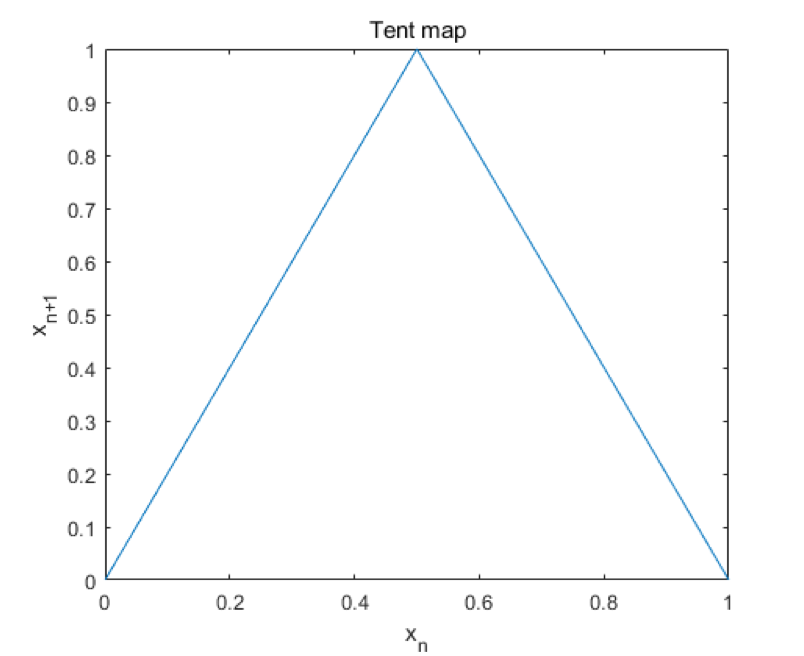
\includegraphics[scale=0.6]{tent_phase.png}
    \caption{帐篷映射的相图($\alpha=\frac{1}{2}$)}
    \label{fig:tent_pha}
\end{figure}

帐篷映射的动力学过程可以看作是在相空间$(0,1)$上的点拉伸再折叠的过程,如图\ref{fig:tent_dyna},帐篷映射可以看作两次映射的复合,第一次映射将$AB$区间上的点拉伸为$A'B'$,相空间从$(0,1)$拉伸到$(0,2)$,点$0$、$0.5$、$1$分别映射为$0$、$1$、$2$;第二次映射将$A'B'$区间上的点拉伸为$A''B''$,相空间从$(0,2)$压缩到$(0,1)$,点$0$、$1$、$2$分别映射为$0$、$1$、$0$。两次映射的拉伸与折叠过程完成了相空间$(0,1)$到其自身的映射。在该过程中,存在一些关键的“转折点”,如第一次映射的$x=0.5$与第二次映射的$x=1$,且相空间的性质随这些点呈对称分布。
\begin{figure}[!]
	\centering
	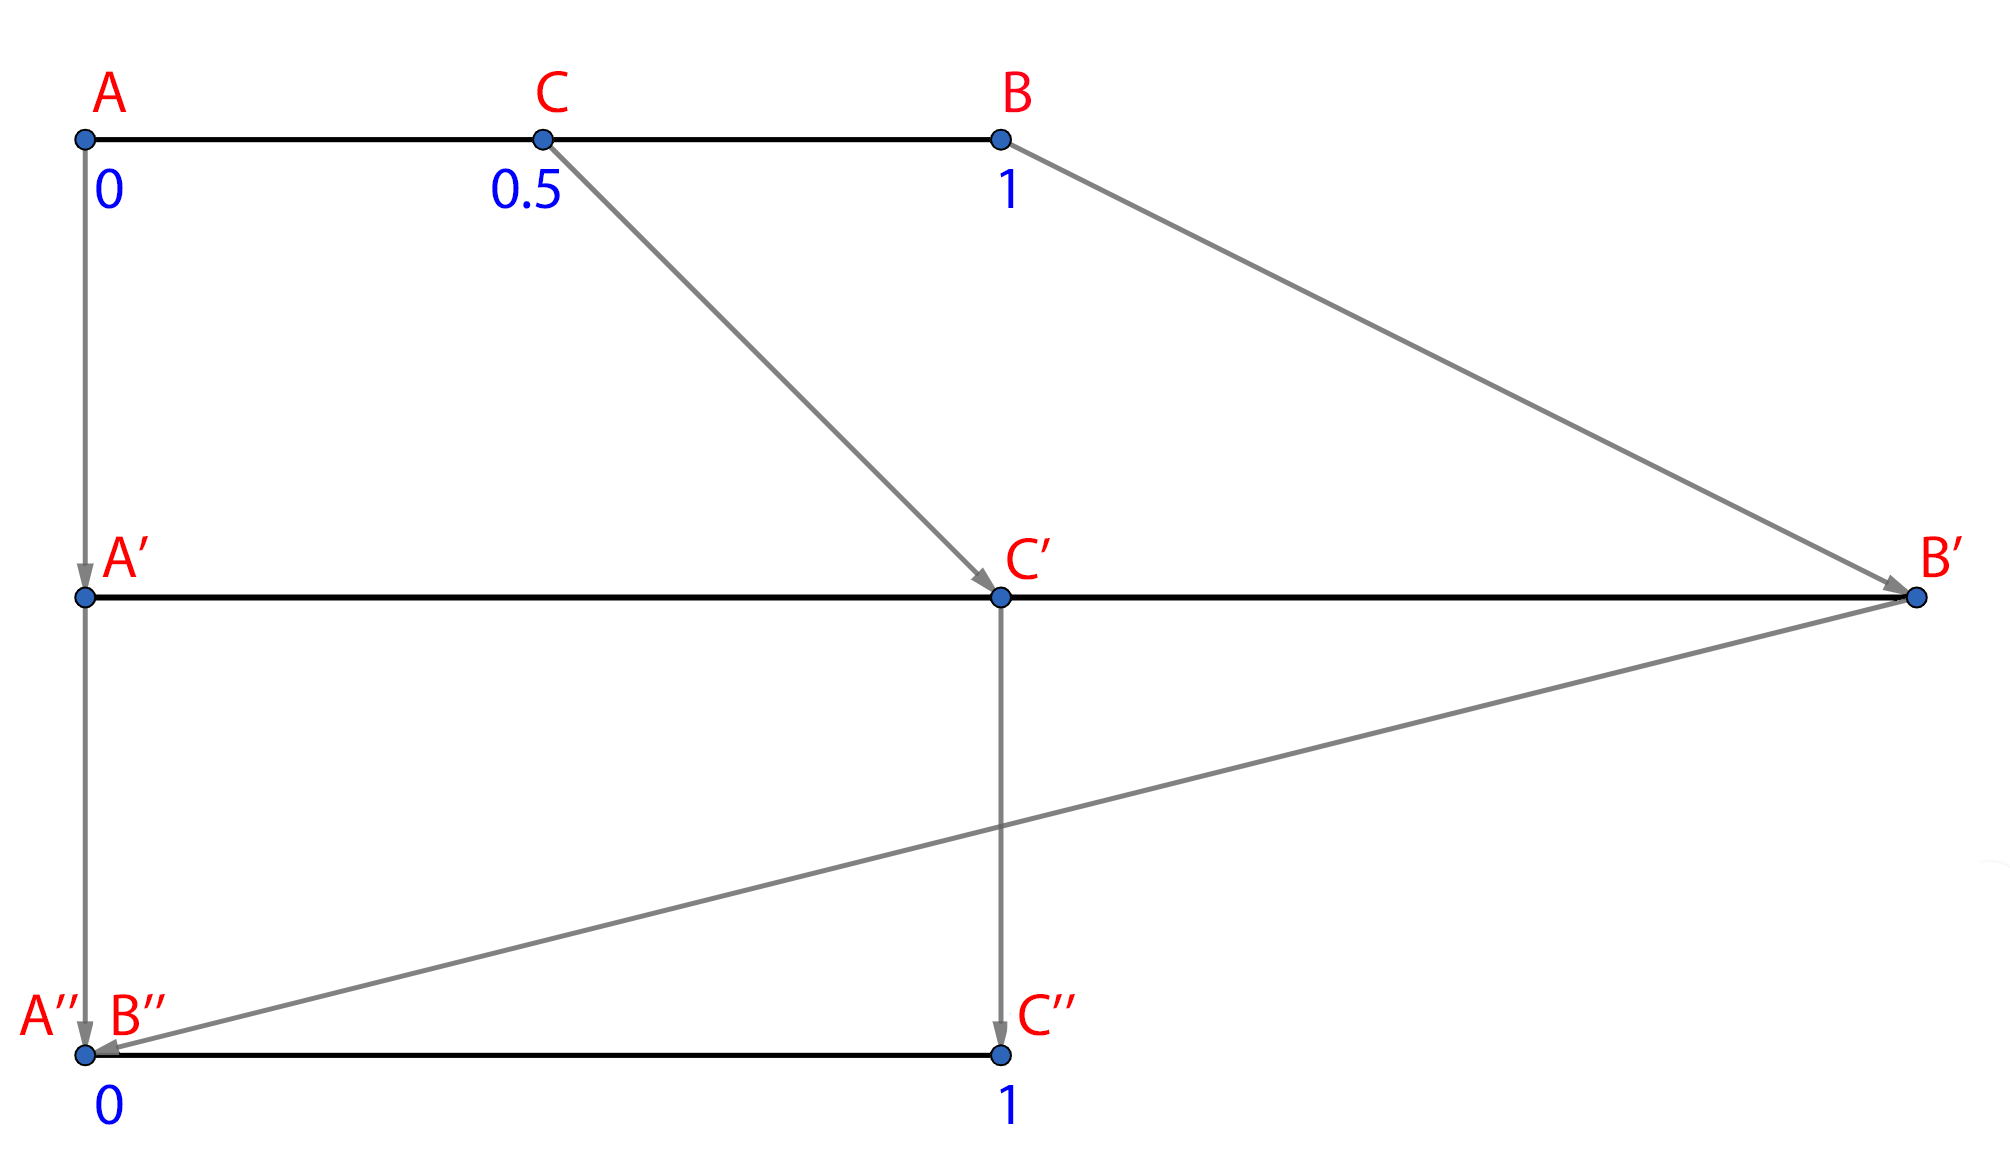
\includegraphics[scale=0.15]{tent/tent_dynamic.png}
    \caption{帐篷映射的映射过程}
    \label{fig:tent_dyna}
\end{figure}


\subsection{帐篷映射的Koopman算符本征函数}
在上一章中的介绍中,我们探究了Koopman算符的本征函数与动力学系统的特征,帐篷映射作为一个较简单的一维分段线性映射,其动力学特征也容易探究,我们将以帐篷映射为例探究Koopman算符的本征值与本征函数与动力学特征的关系及对相空间的划分。


\subsubsection{正交完备基函数空间}
在式\eqref{eq:Koop_kl1}中,我们得到了Koopman算符的矩阵表示,选取一定参数:演化格点数量$n=1000$,函数格点数量即基函数数量$m=4$,依此我们可以计算矩阵$U$的本征值与本征函数。通常我们会得到许多本征值与本征函数,且本征值与本征函数的数量取决于函数格点的数量。而我们在上一章中提到了,关于本征值与本征函数,我们更关心接近1的本征值与对应的本征函数,因为其反映了相空间中一条随时间演化不变的轨道。我们可以将本征函数值的大小(若非特殊说明,当本征函数为复数时我们取其实部作为大小)画在相空间中,通过将本征函数与相空间对应来探究其关系。

图\ref{fig:tent_eig_RGFL}画出了$n=1000$,$m=4$时,四种不同的基函数下(矩形窗局函数、高斯基函数、傅里叶基函数、勒让德基函数)帐篷映射的本征函数,其中每个基函数下又包含4个不同的本征值对应的本征函数。四种基函数的分布见图\ref{fig:func_bas}。
\begin{figure}[!]
    \centering
    \subfloat[矩形窗基函数]{
      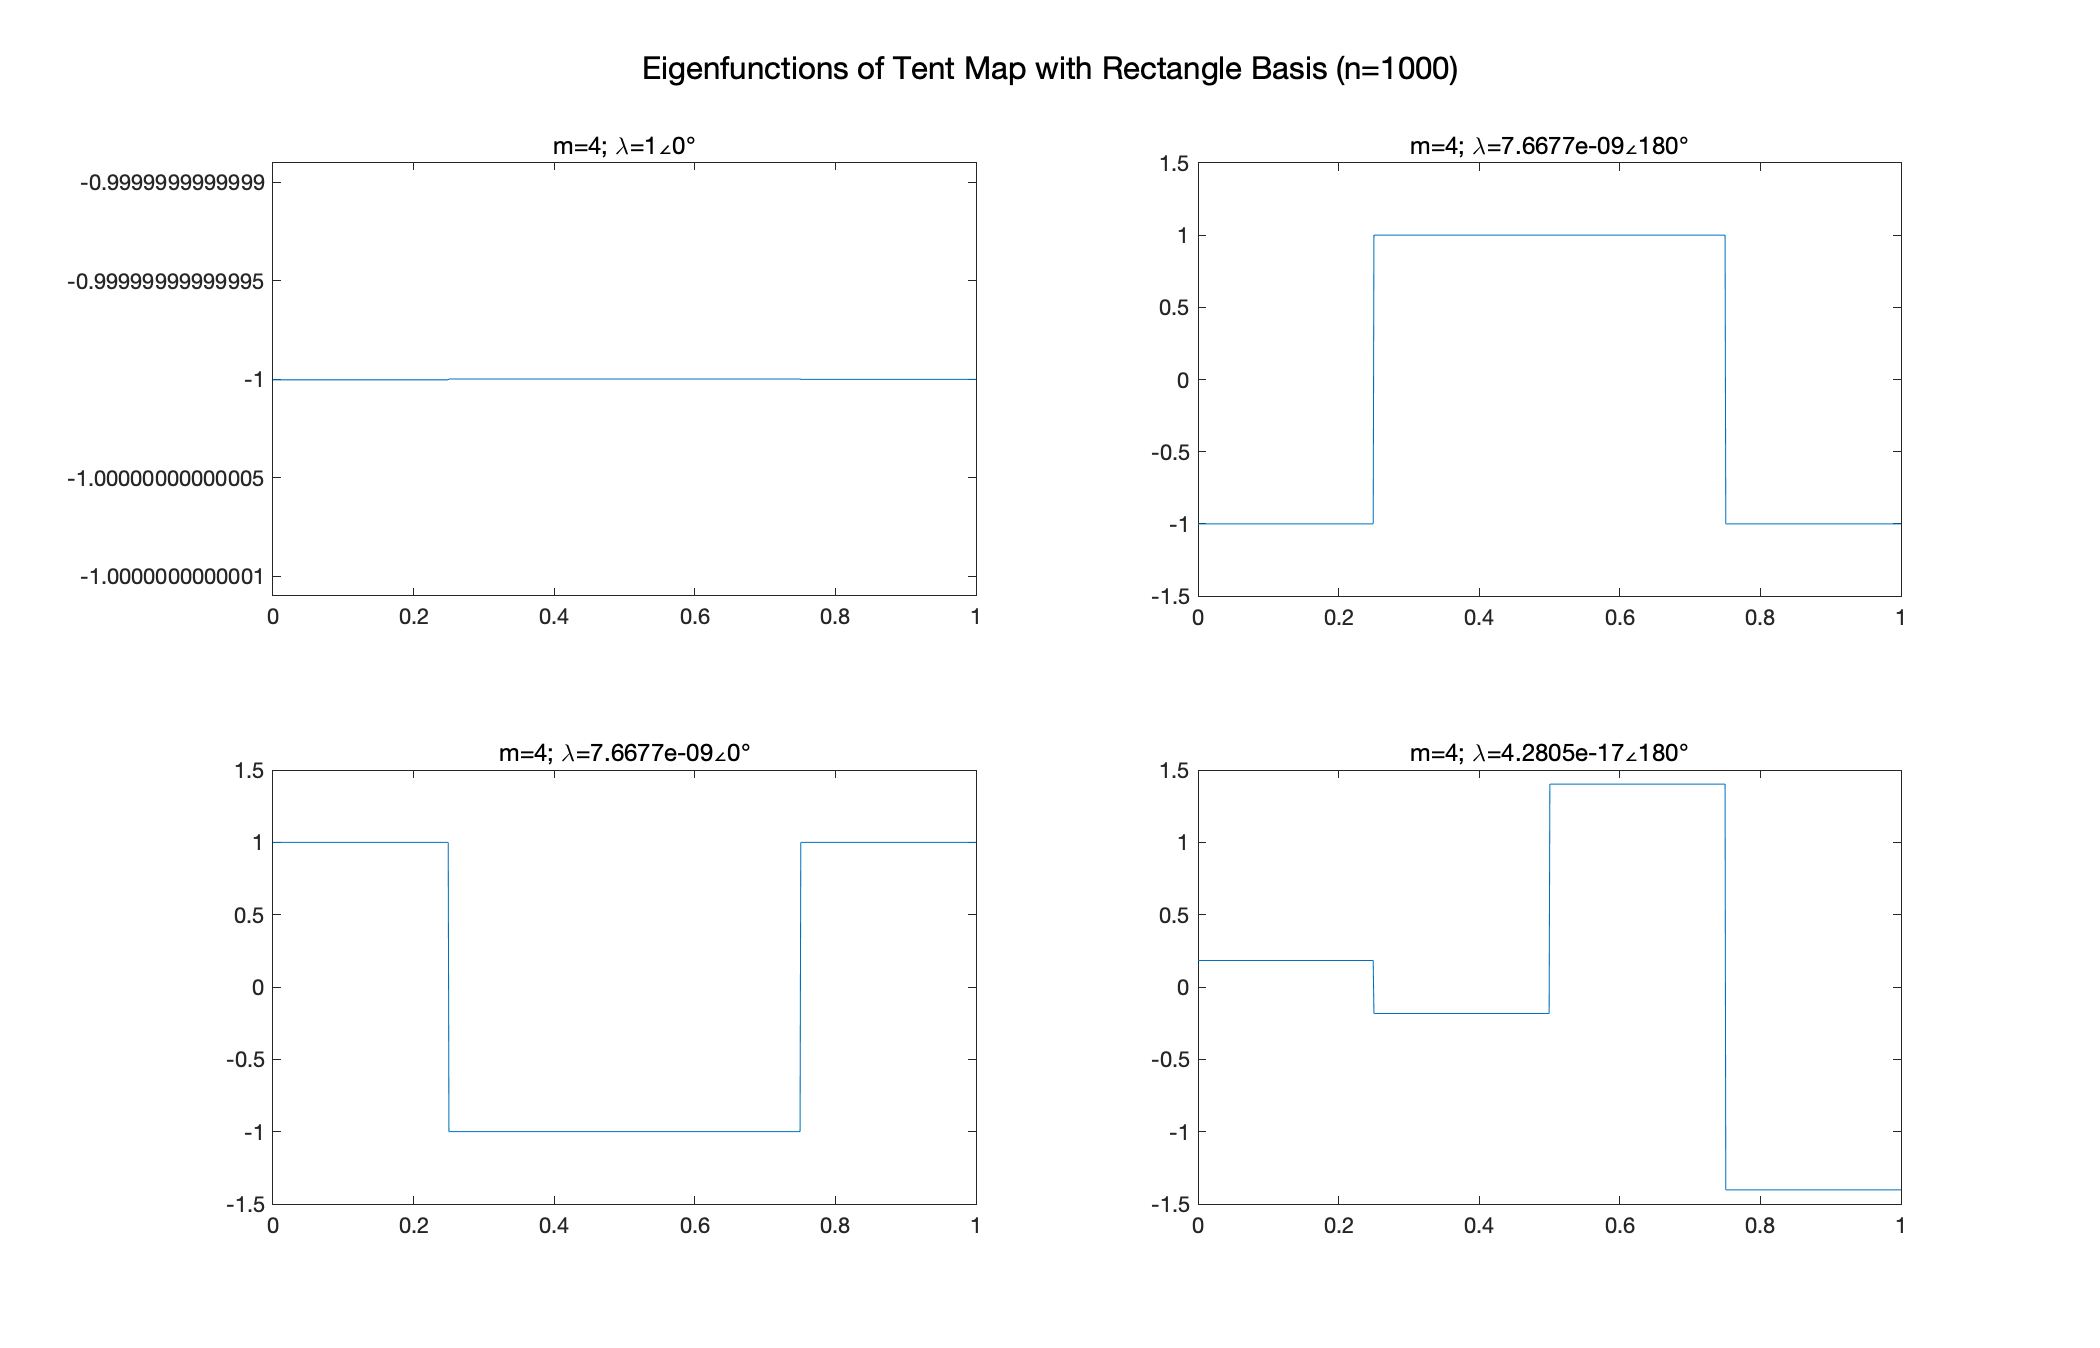
\includegraphics[scale=0.2]{tent/Tent_eigen_Rectangle_n1000_m4}}
    \subfloat[高斯基函数]{
      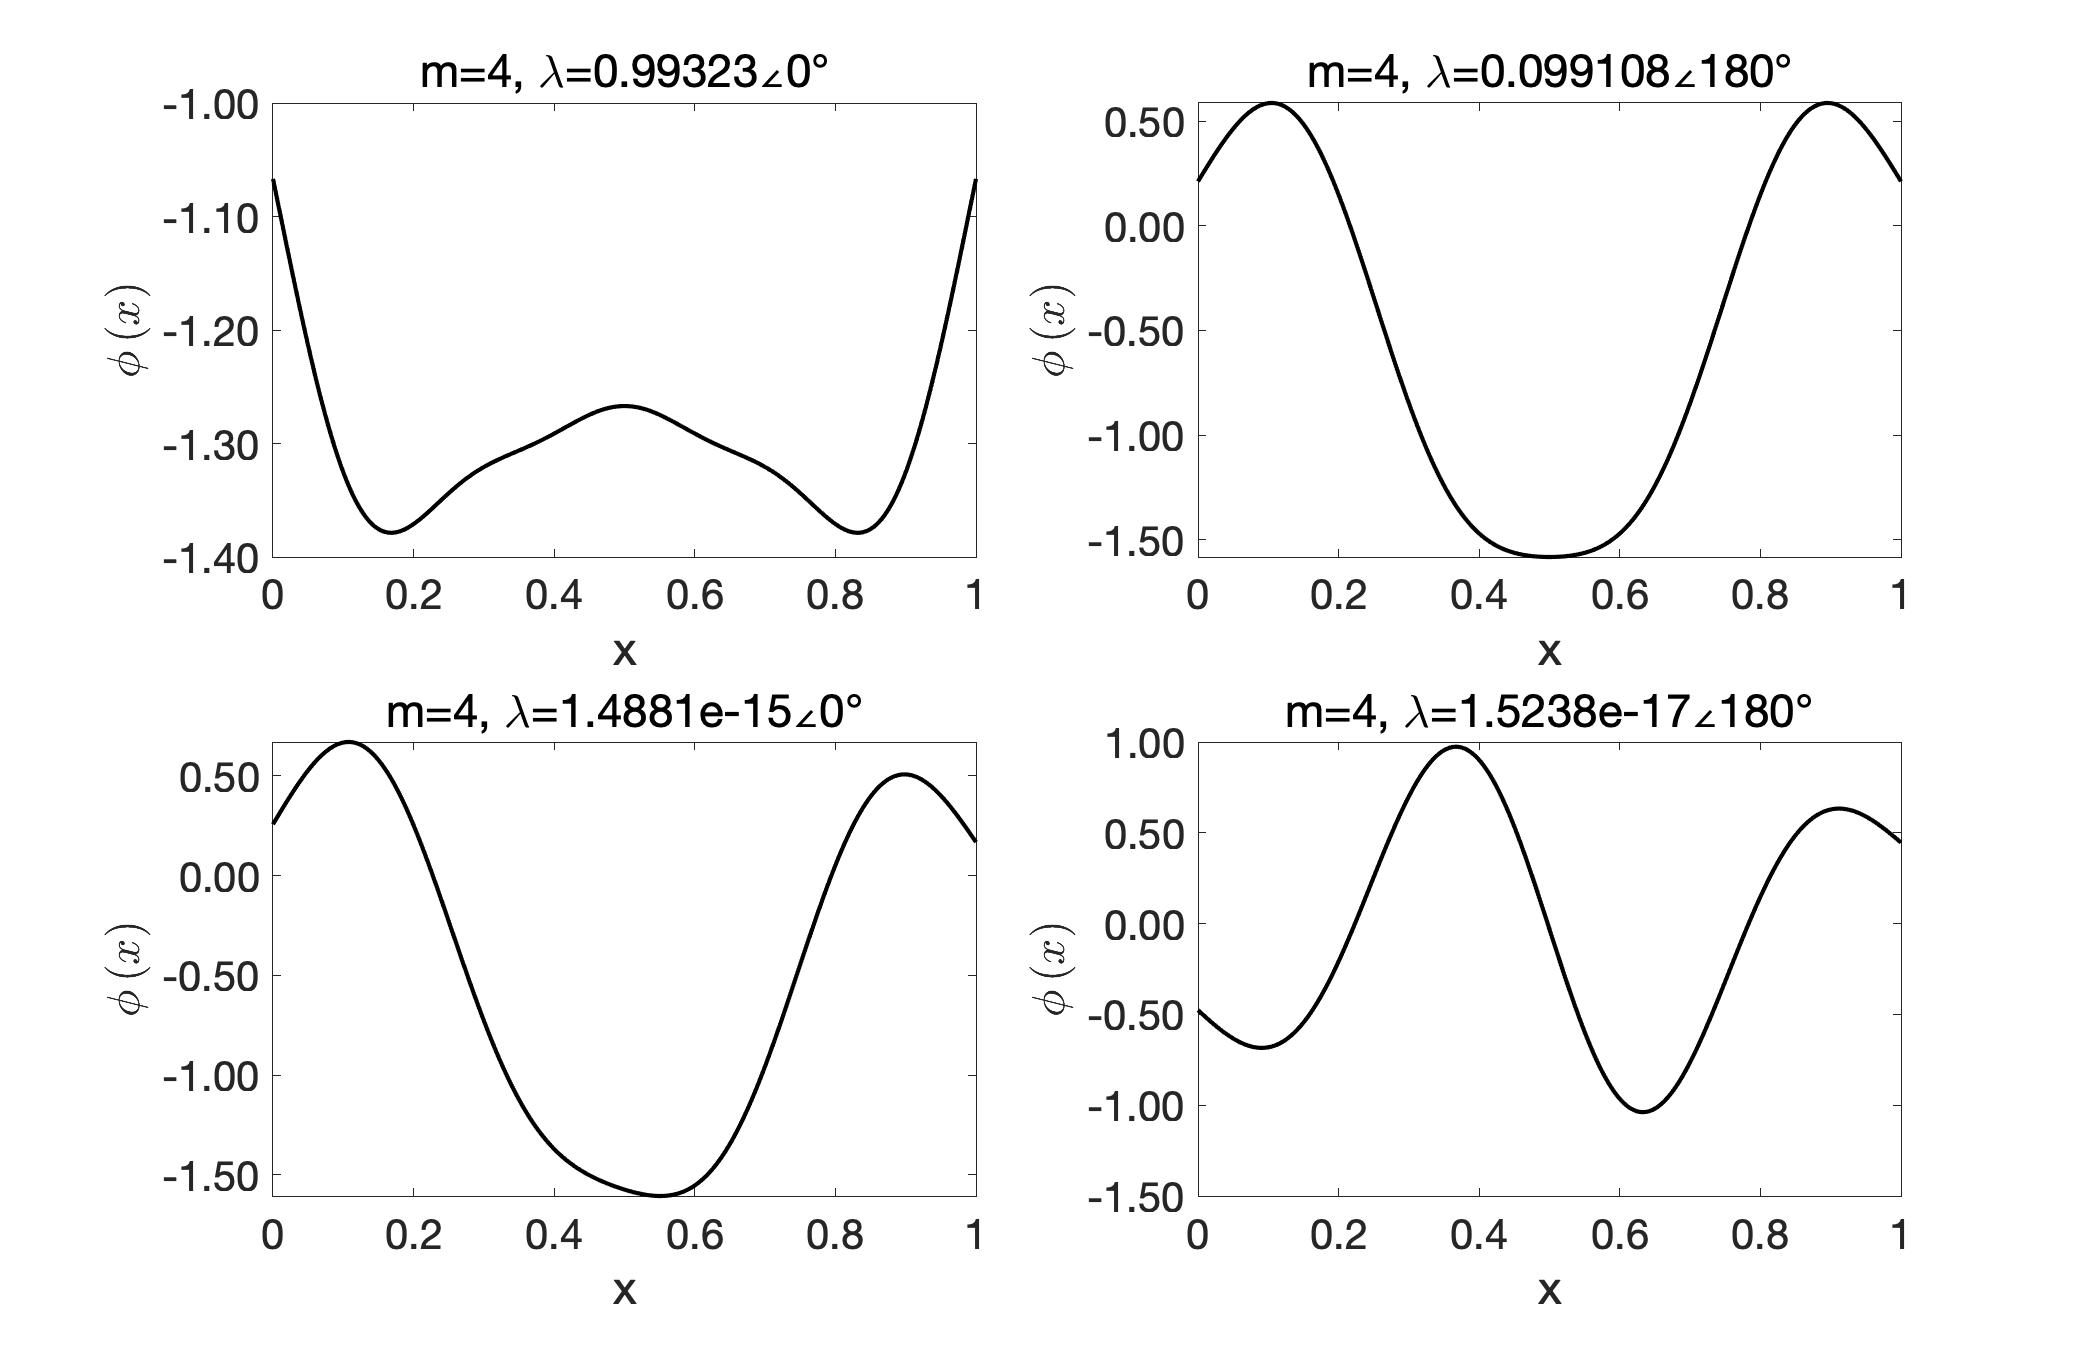
\includegraphics[scale=0.2]{tent/Tent_eigen_Gauss_n1000_m4}}
      \\
    \subfloat[傅里叶基函数]{
      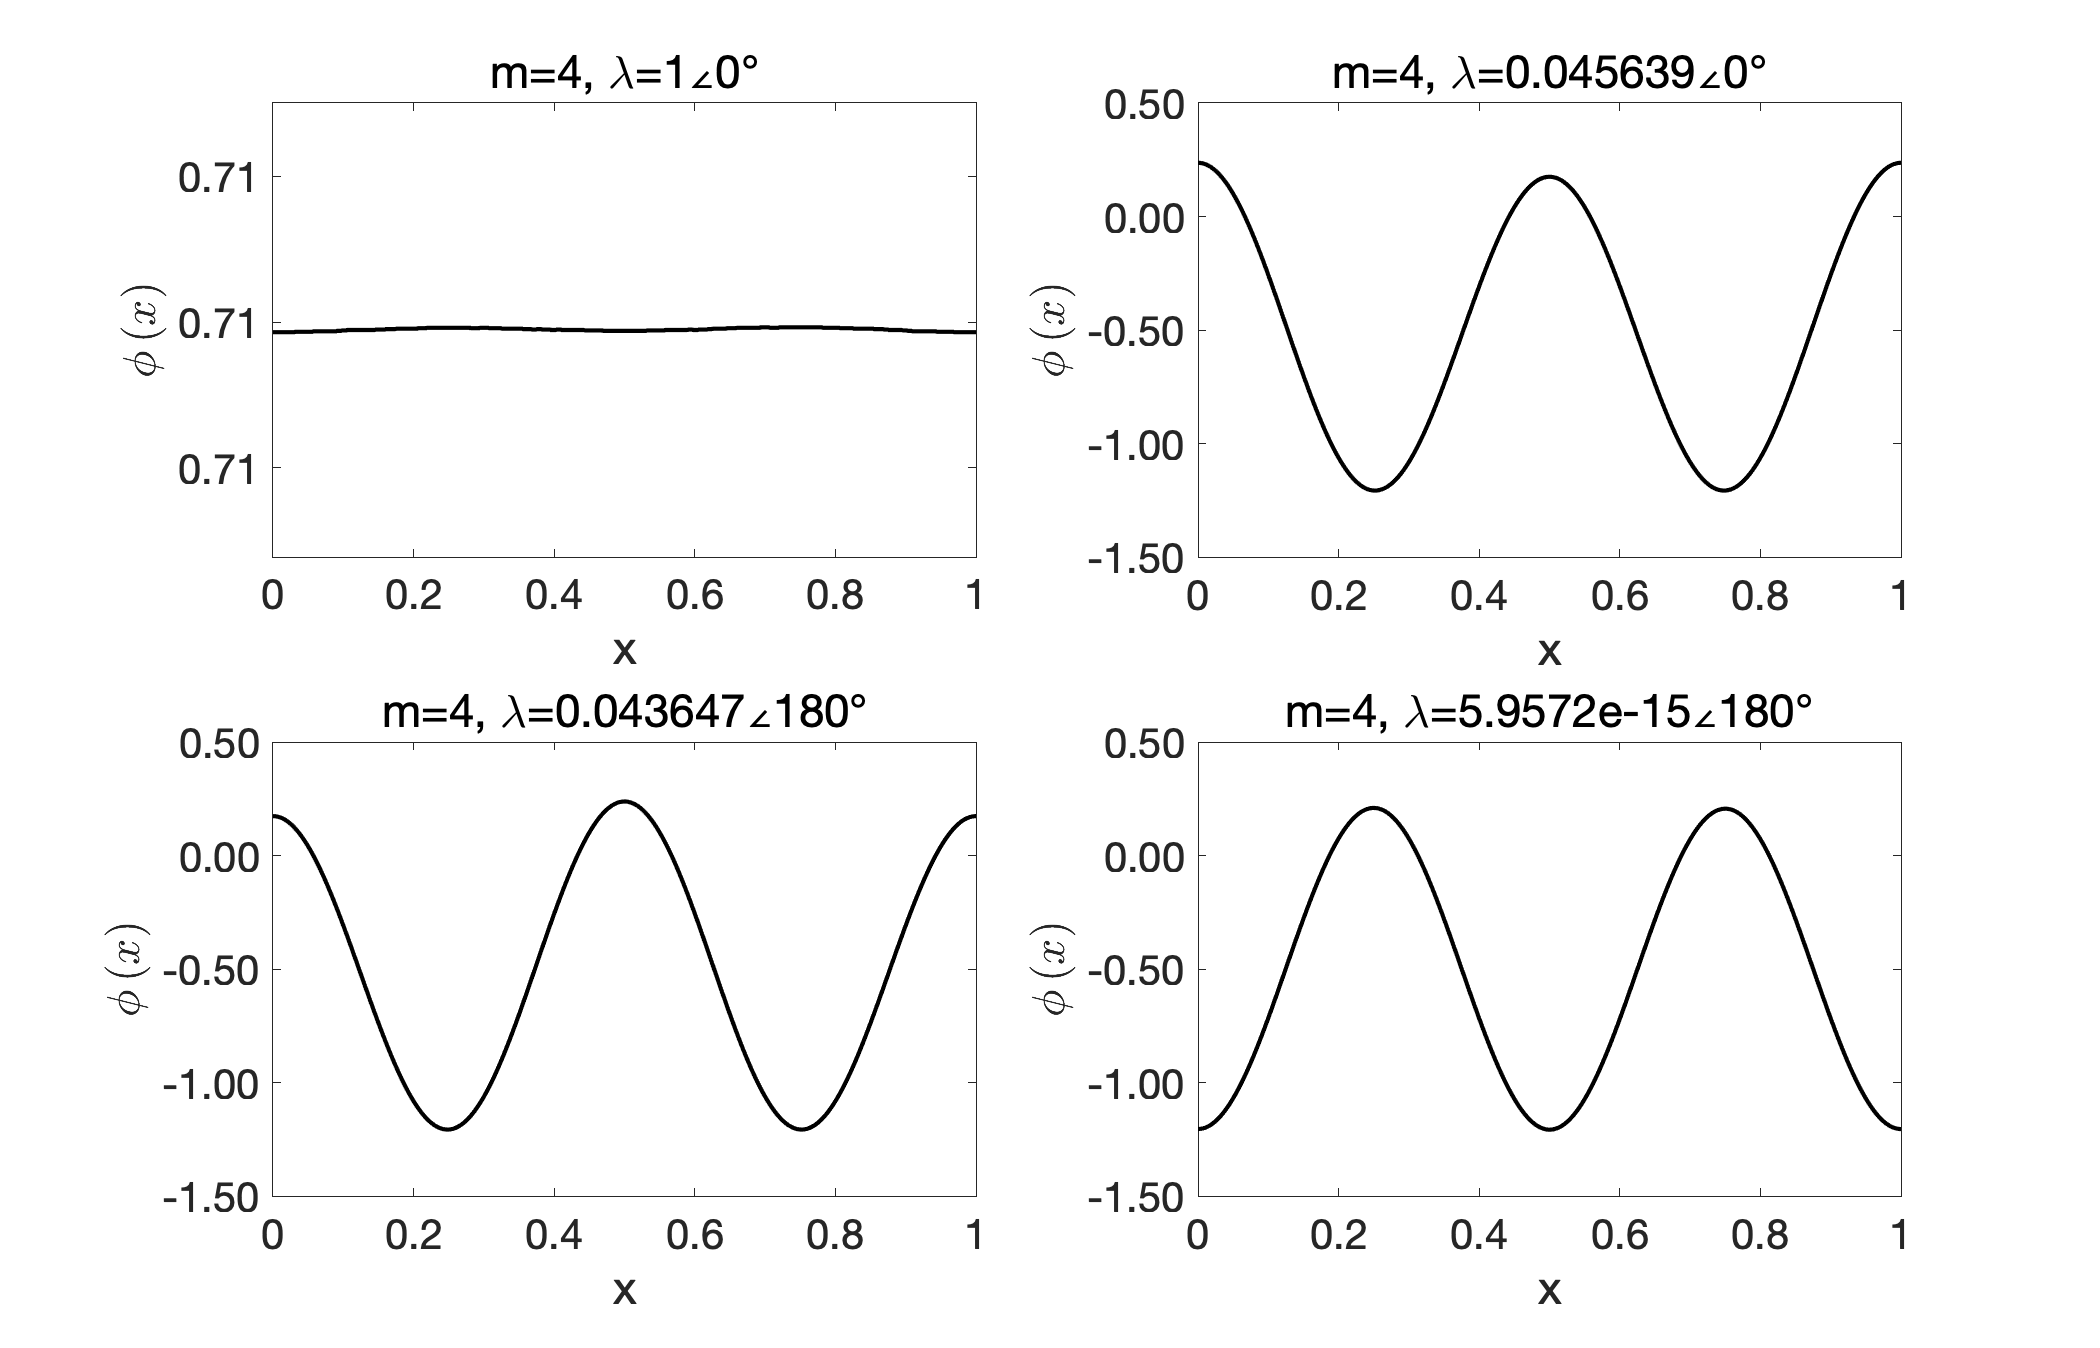
\includegraphics[scale=0.2]{tent/Tent_eigen_Fourier_n1000_m4}}
    \subfloat[勒让德基函数]{
      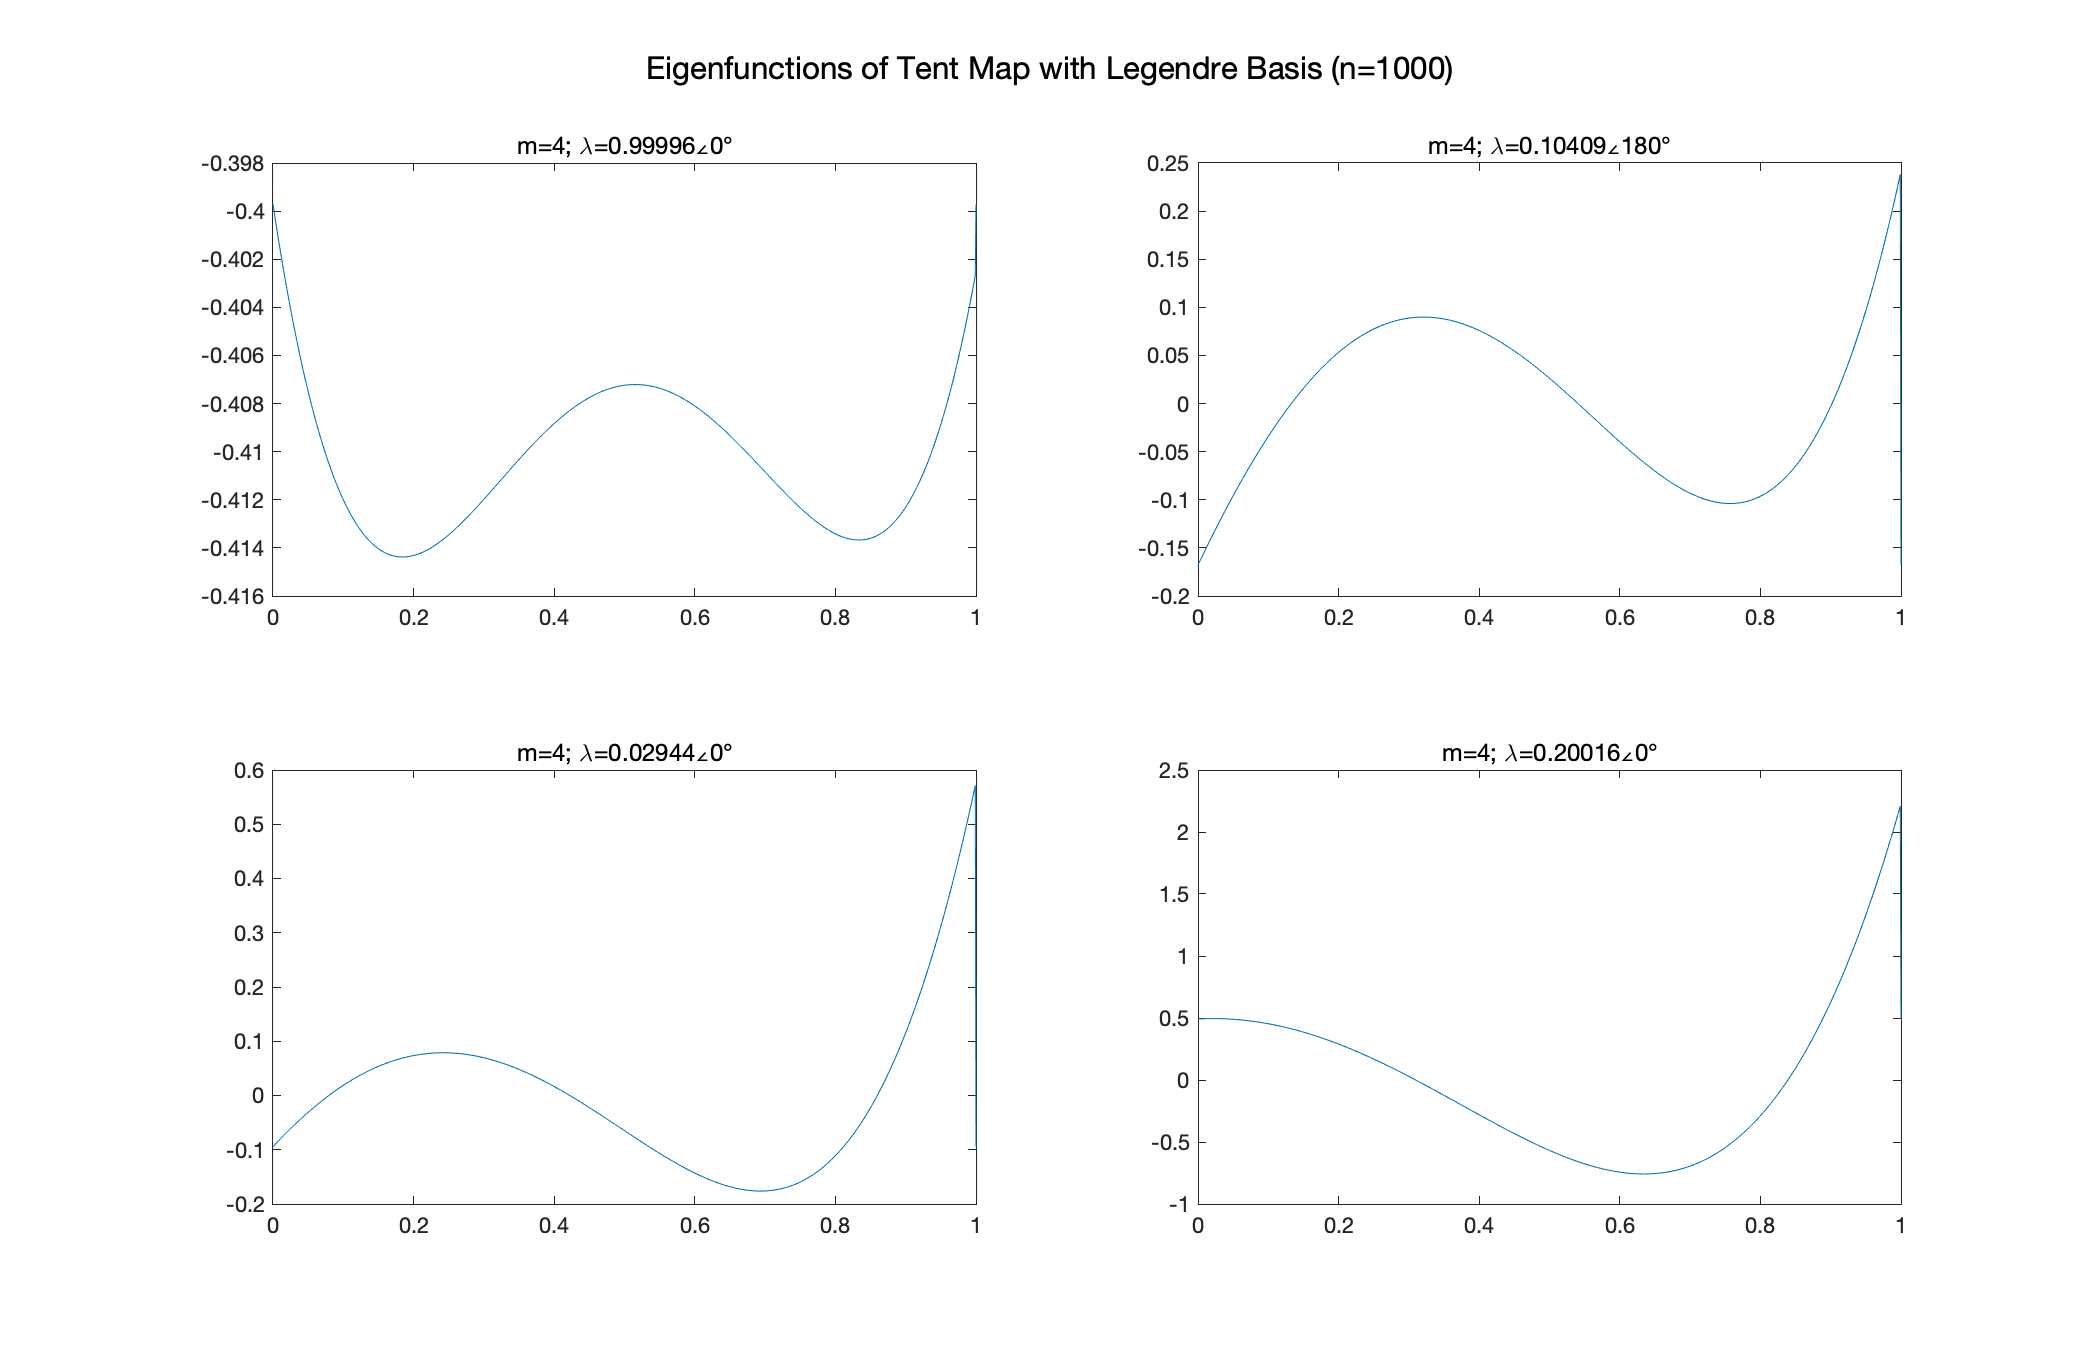
\includegraphics[scale=0.2]{tent/Tent_eigen_Legendre_n1000_m4}}
    \caption{四种基函数下帐篷映射的本征函数($m=4$)}\label{fig:tent_eig_RGFL}
\end{figure}
从图\ref{fig:tent_eig_RGFL}中我们可以发现,在不同的基函数下,Koopman算符的本征函数表现出极大的差异,这也可以从本征函数与基函数之间的关系中可以得出:本征函数总是在选取的基函数空间内,即从数学上每个本征函数都由所有的基函数线性组合而成。图中取$m=4$时,其函数空间是相当不完备的,只能表示很有限的函数,因此我们的本征函数只是在此函数空间上的一个近似(或者说是函数几何空间从高维到低维的投影),因此基函数的选取会影响本征函数空间,因此我们对基函数的选取亦至关重要。为了能更好的划分出相空间,我们应尽量体现出不同基函数的作用,以此对相空间进行划分,如矩形窗基函数、高斯基函数同属局部(或近似局部)函数,这种局部函数能通过每个基函数比例系数的大小来体现对相空间的划分,因此我们更关心这种局部函数,在后面的计算中也会更多的使用高斯基,以此来体现本征函数对相空间的划分。

在图\ref{fig:tent_eig_RGFL}中,每个子图中都包含4个不同的本征值及其对应的4个本征函数图像,且其中包含一个$\lambda\approx 1$的本征值,在之前的讨论中,我们认为本征值接近1的本征函数反映了相空间中一条随时间演化不变的轨道。而我们在矩形窗基函数和傅里叶基函数中也确实看到了这样的常函数轨道。而其他的本征值则不趋于1,这也可以从我们对函数空间选取的不够完备去考虑:我们不可能选取一个完全完备的函数空间,我们的本征函数只是在此函数空间的一个近似。

基函数数量的不同同样也是影响本征函数的一个重要因素。图\ref{fig:tent_eig_RGFL}中画出了$m=4$时的本征函数,当$m$取不同值时,如$m$越来越大时,意味着我们的函数空间的维度更高,可以描述的本征函数的维度也就越高,则对于局部函数如高斯函数而言,我们描述本征函数的精细度就更高,于是我们可以提高基函数数量$m$的大小,用以描述更精细的本征函数。但这也会使我们得到的本征函数的数量有所增加,当我们将关心的本征函数聚焦为$\lambda\approx 1$时,我们可以将不同基函数数量的本征函数画出,如图\ref{fig:tent_eig_RGFL_multim}中,我们取四种基函数及基函数数量$m=2,3,4,8,10,16,20,50,100$时对应的本征值与本征函数,以此来反映出随着函数空间的精细度的提高本征函数的变化。

\begin{figure}[!]
  \centering
  \subfloat[矩形窗基函数]{
    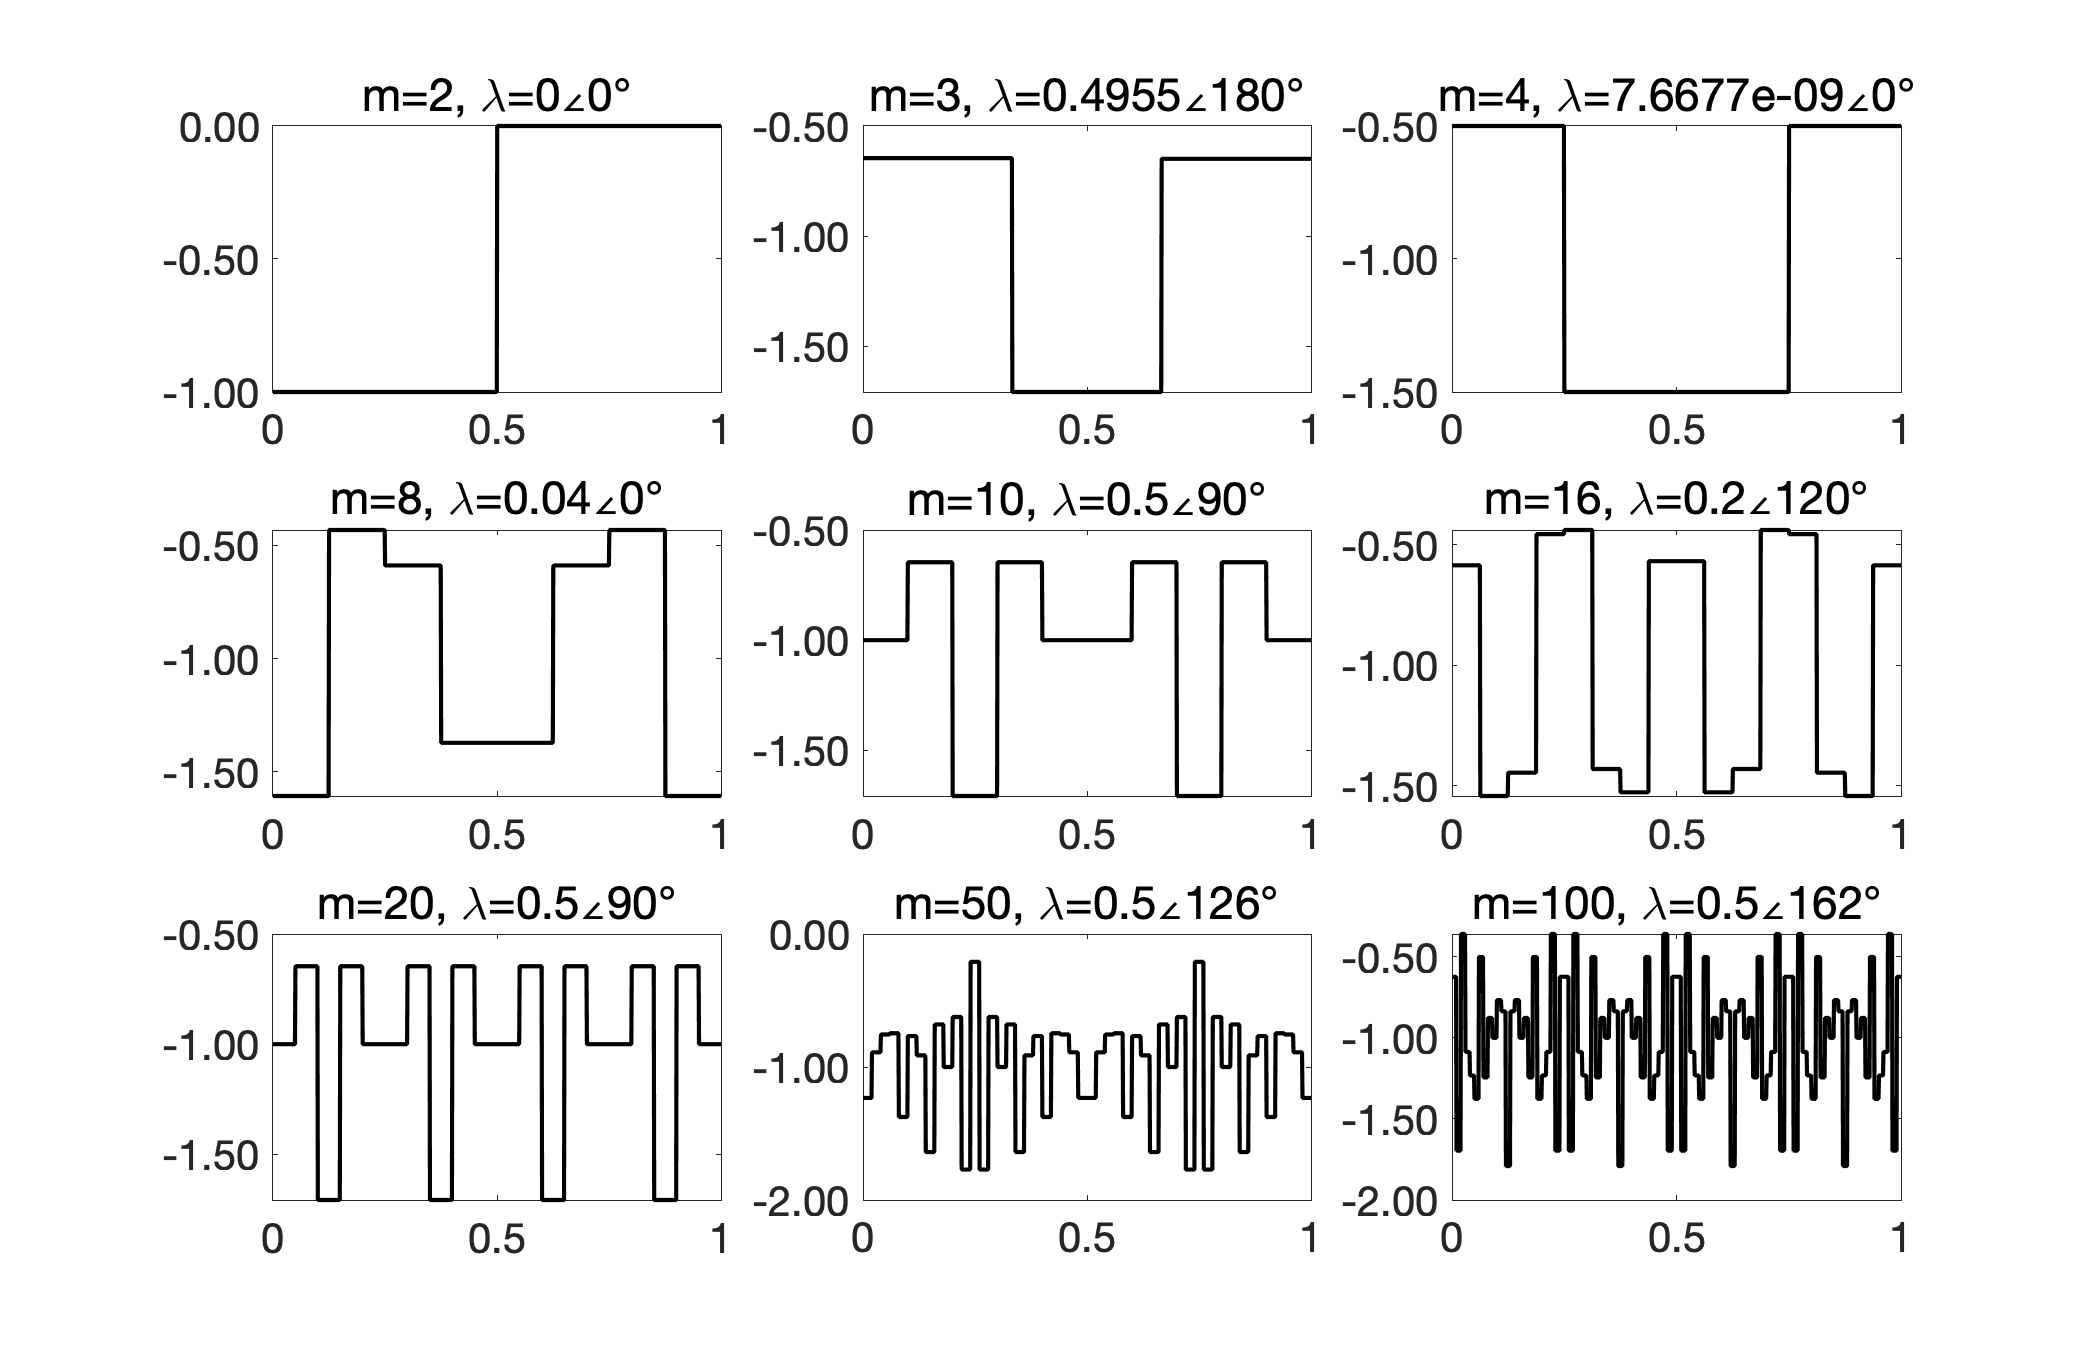
\includegraphics[scale=0.2]{tent/Tent_eigen_Rectangle_n1000_m2-3-4-8-10-16-20-50-100}}
  \subfloat[高斯基函数]{
    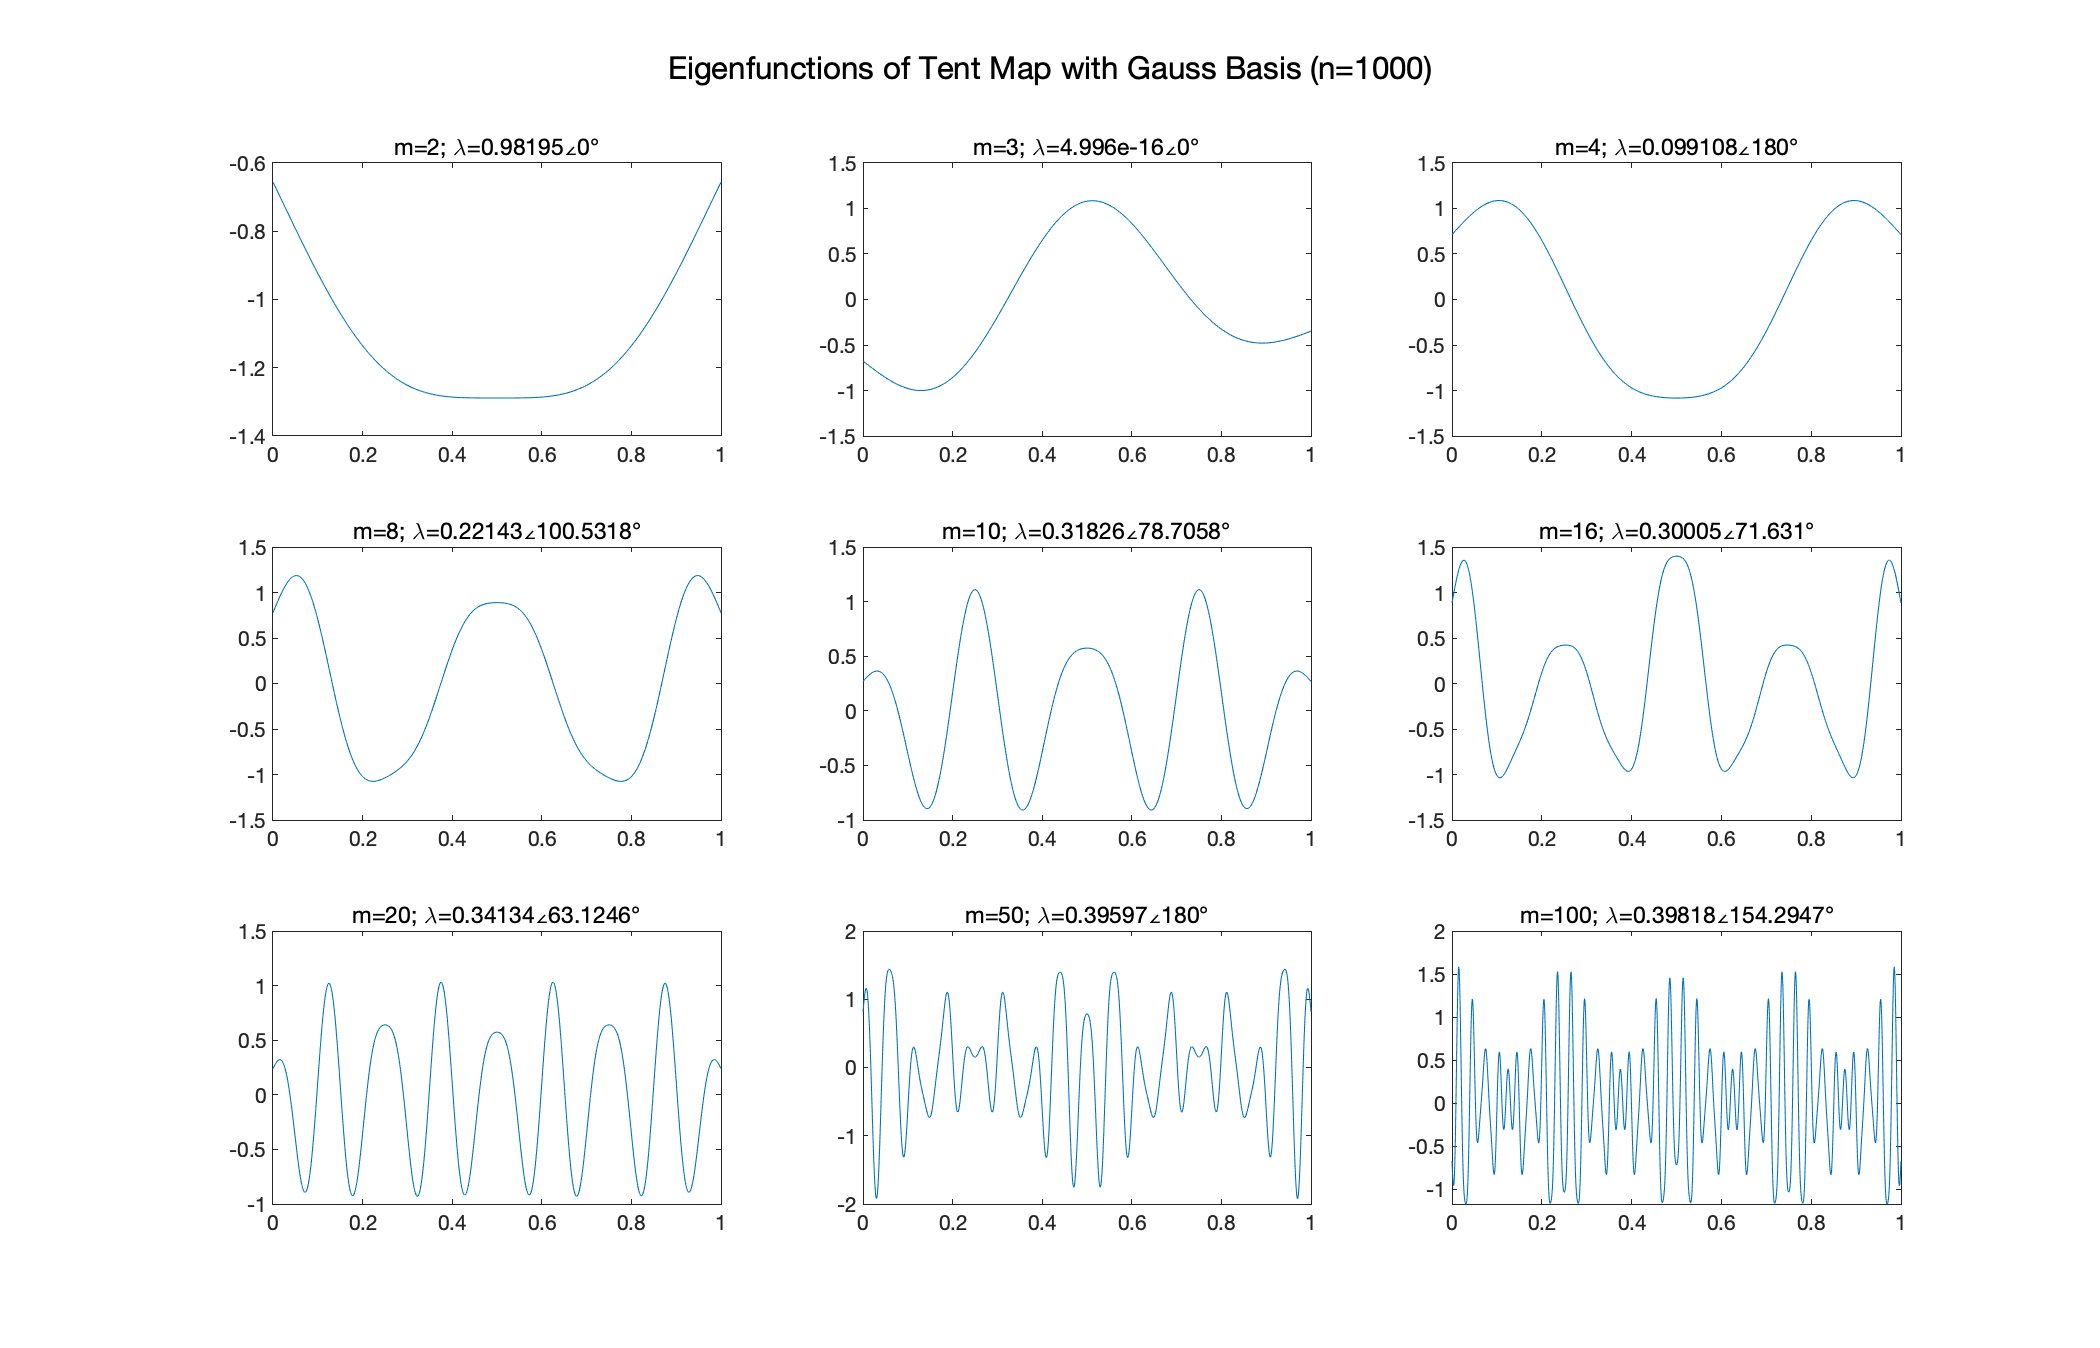
\includegraphics[scale=0.2]{tent/Tent_eigen_Gauss_n1000_m2-3-4-8-10-16-20-50-100}}
    \\
  \subfloat[傅里叶基函数]{
    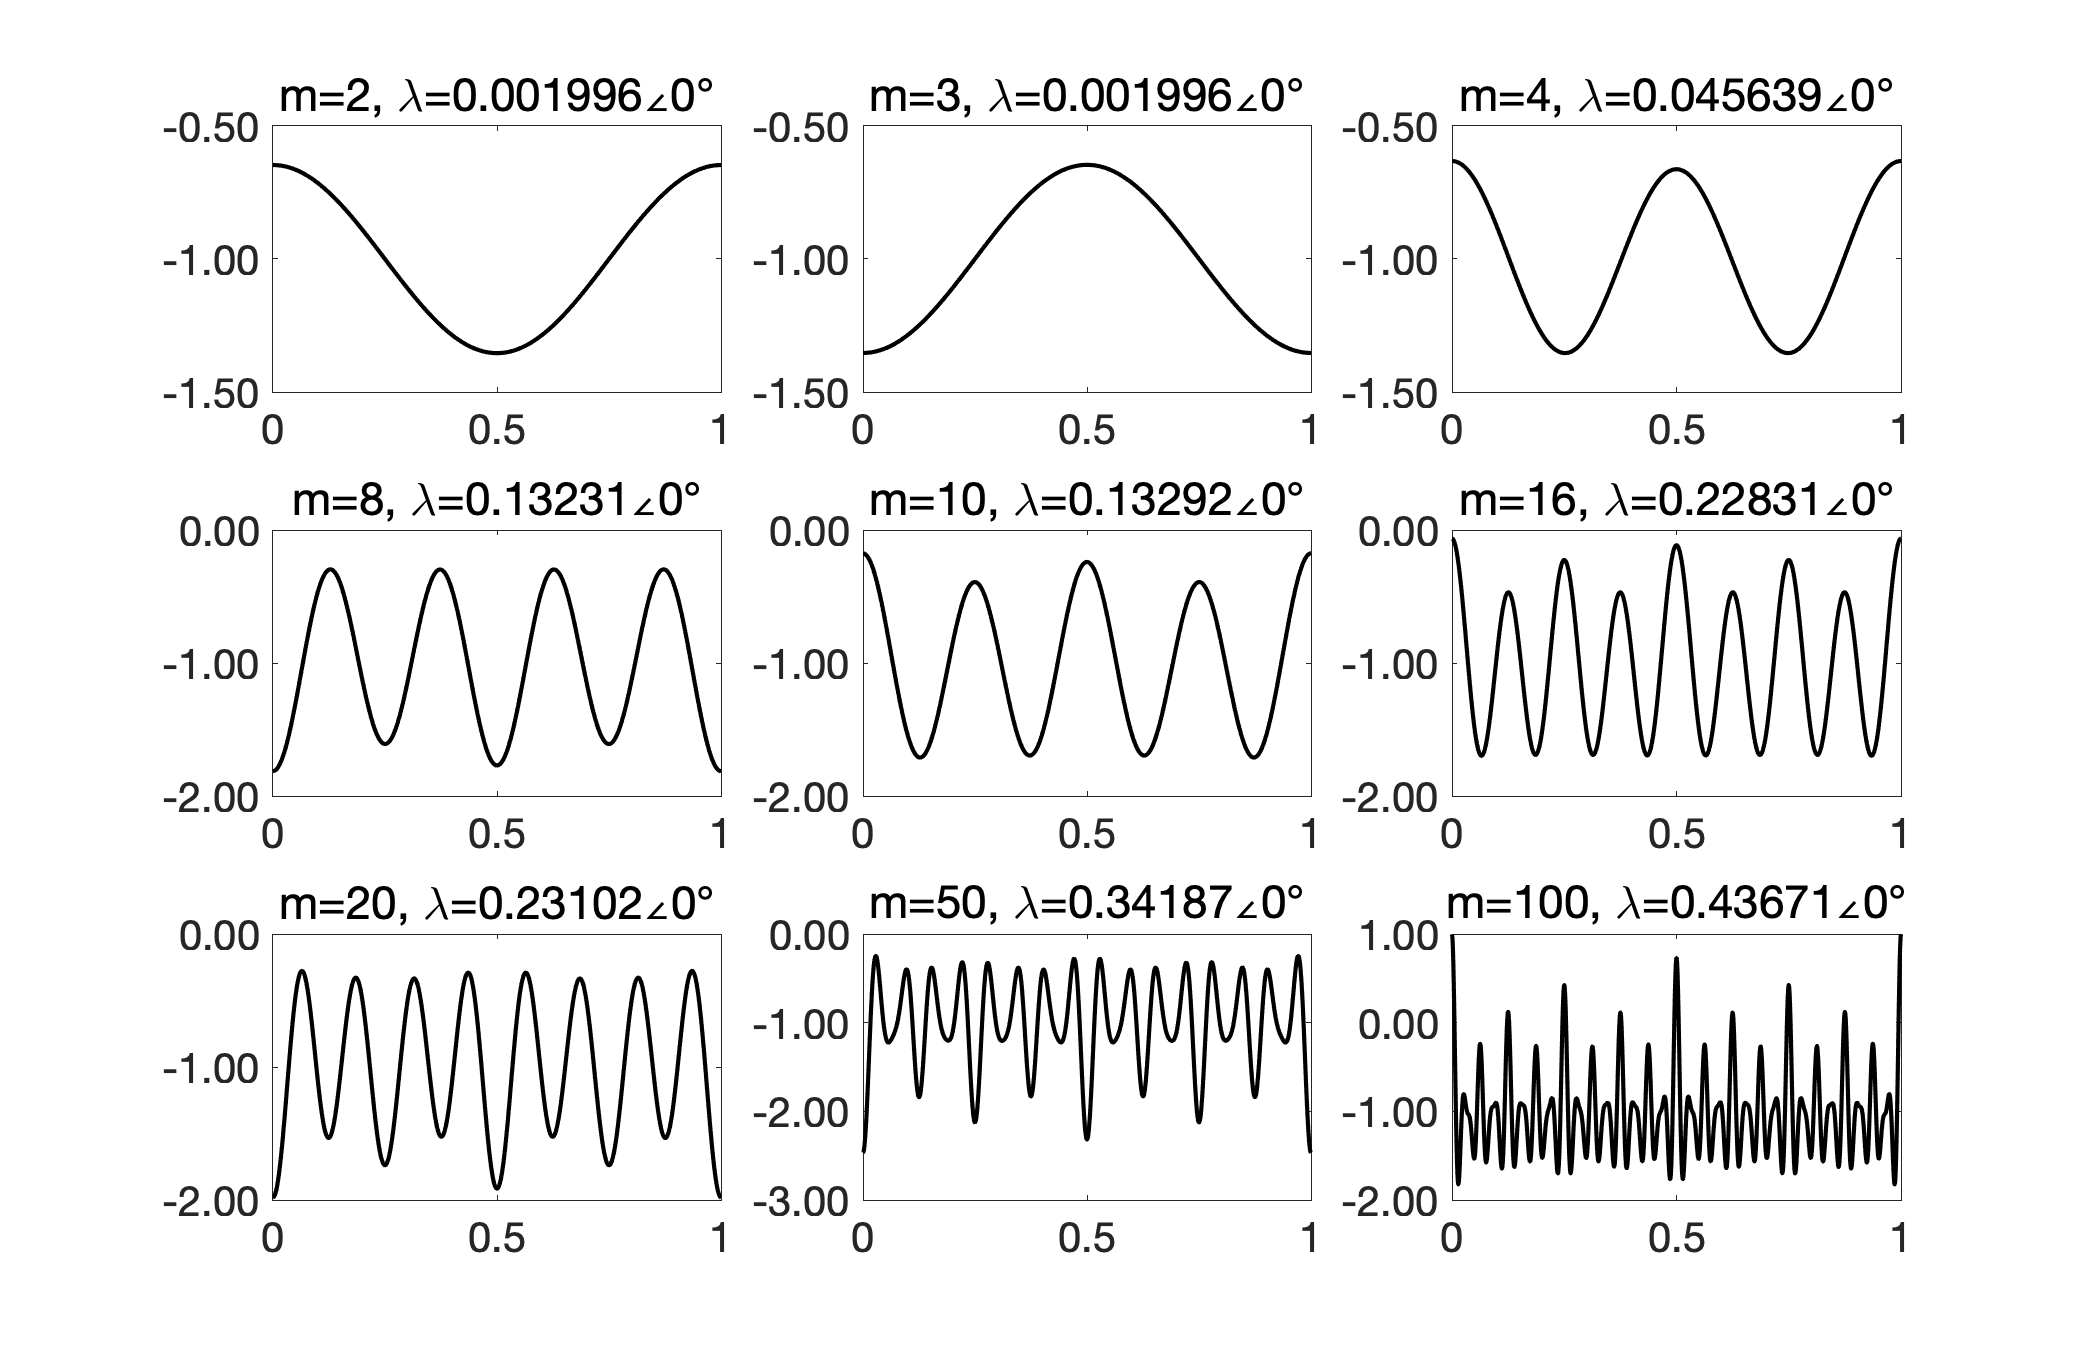
\includegraphics[scale=0.2]{tent/Tent_eigen_Fourier_n1000_m2-3-4-8-10-16-20-50-100}}
  \subfloat[勒让德基函数]{
    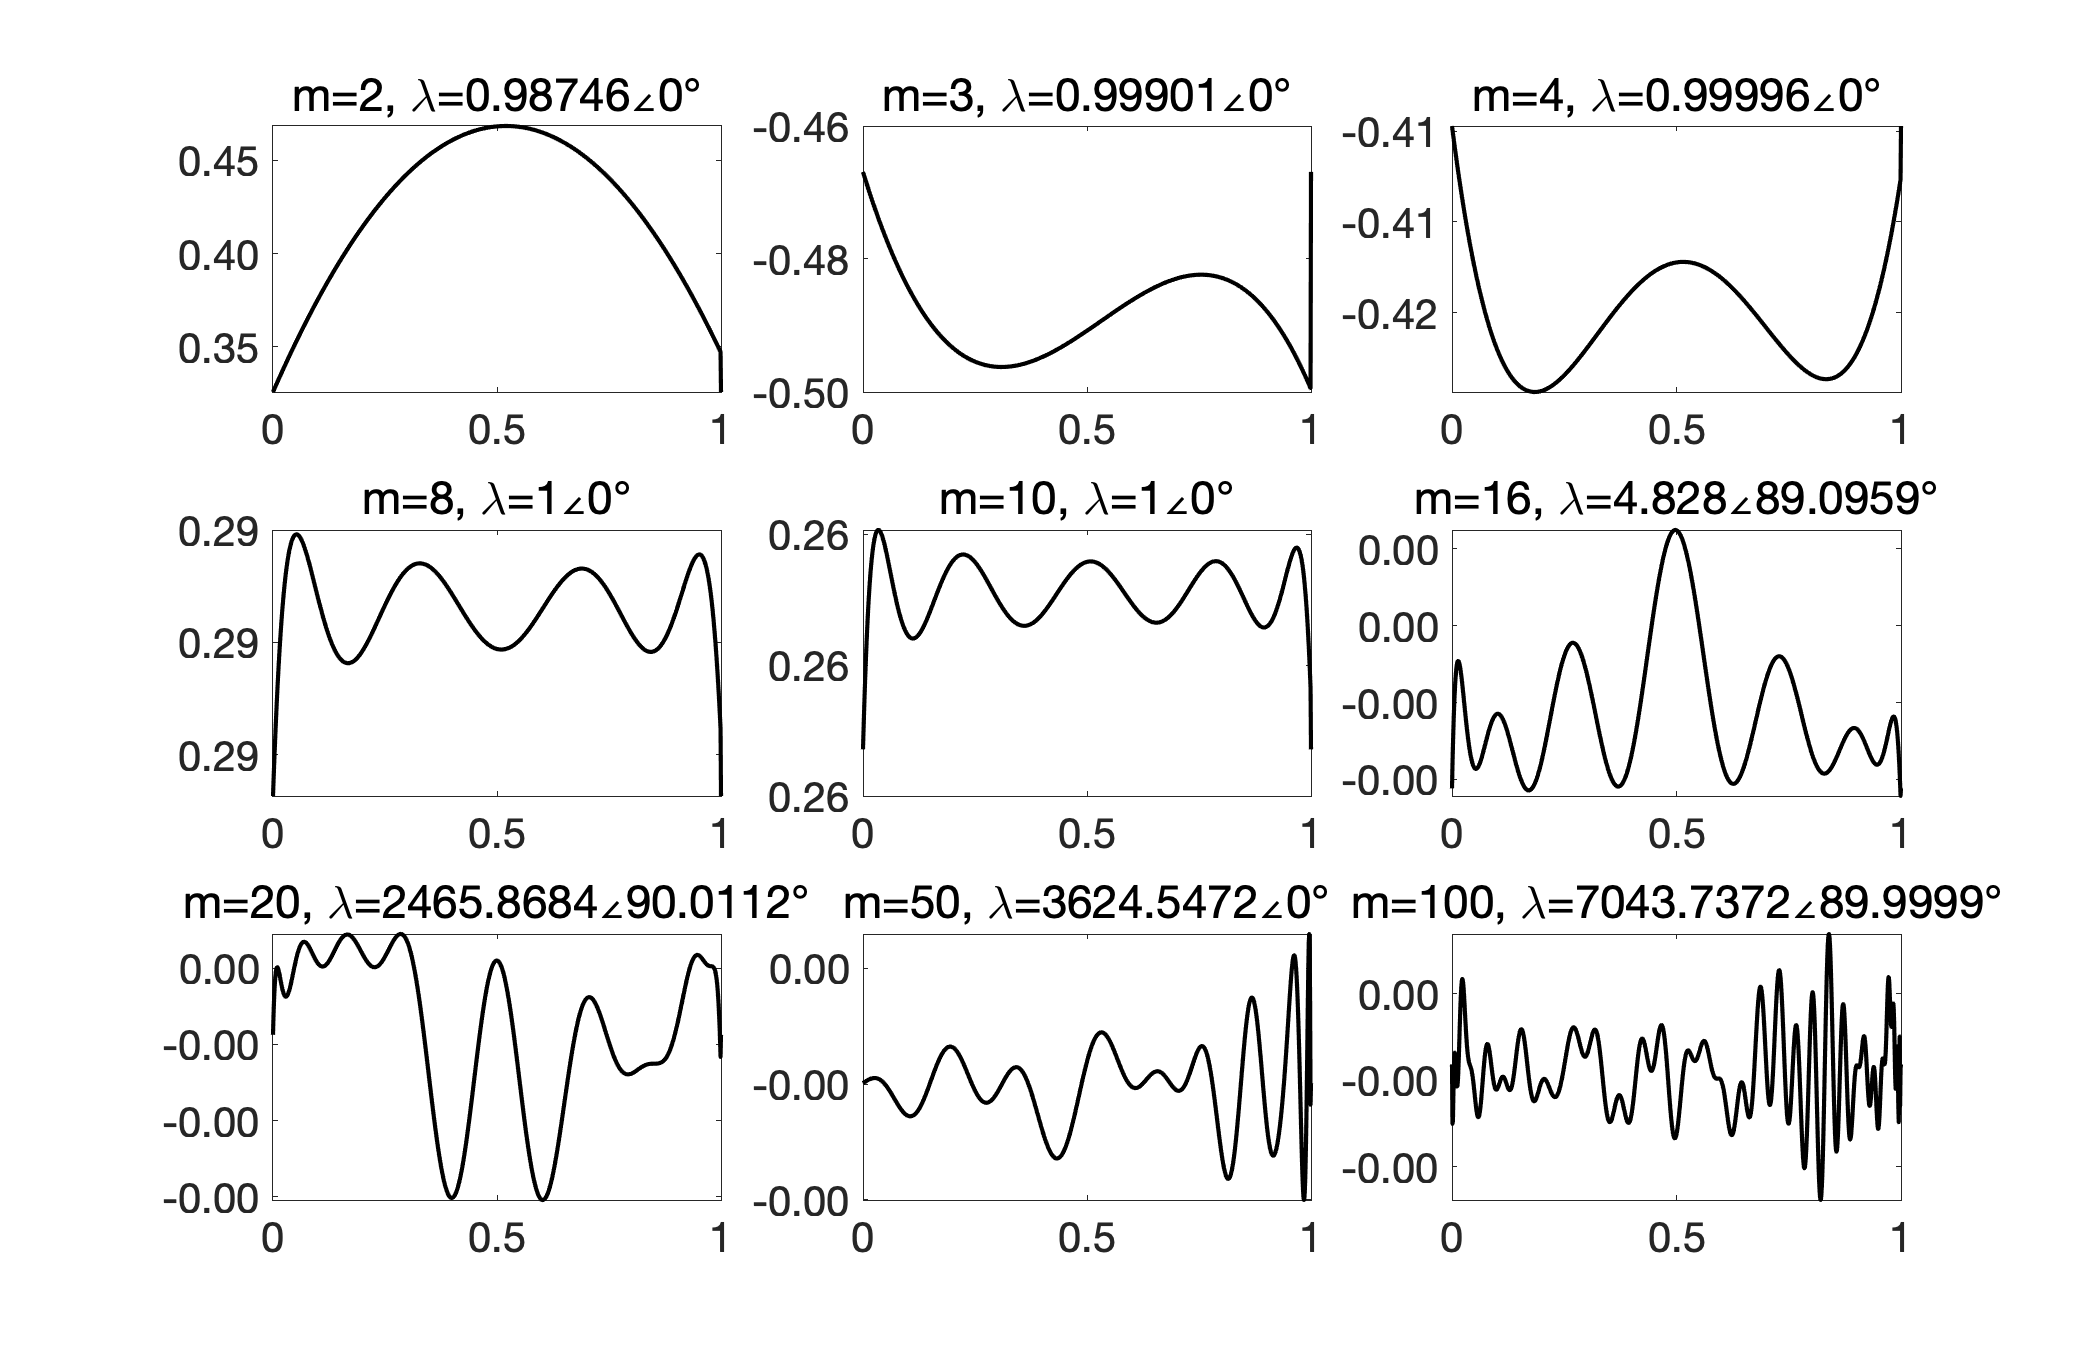
\includegraphics[scale=0.2]{tent/Tent_eigen_Legendre_n1000_m2-3-4-8-10-16-20-50-100}}
  \caption{不同基函数数量下帐篷映射的本征函数}\label{fig:tent_eig_RGFL_multim}
\end{figure}

在图\ref{fig:tent_eig_RGFL_multim}中,我们确实可以发现,当基函数数量增加时,本征函数图像的频率增加了,即描述本征函数的精细度增加了。且本征函数的变化有一定的规律:如在高斯基函数中,当$m=2$时,函数有一个近似$x=0.5$的极值点,而此极值点在其他m值时一直存在,同样$m=3$多出的两个极值点似乎也并未随着m值的增加而消失,这似乎印证了随着基函数数量的增加而使得描述本征函数的精细度的增加。

从另一个角度,$x=\frac{1}{2}$点似乎具有某种特殊性,其将相空间$(0,1)$分为对称的两部分,而每部分中又有极值点将每个部分各自分为两部分,形成类似分形的本征函数,我们将在后续的讨论中继续探究这些点与本征函数的关系。

\subsubsection{自然基函数空间}
在式\eqref{eq:Koop_kl2}中,我们通过构造自然基函数格点得到了Koopman算符的矩阵表示,选取合适的参数:演化格点$n=1000$,基函数数量$m=4$下,我们可以计算得到4个Koopman算符$U$的本征值与本征函数并将其画到相空间中,如图\ref{fig:Tent_eigen_natural_n1000_m4}。我们可以发现在自然基函数空间下,本征函数的图像变得更为尖锐,但也更接近帐篷映射的相图。且其同样存在一些$x=\frac{1}{2},\frac{1}{4},\frac{3}{4}$的关键点。
\begin{figure}[!]
	\centering
	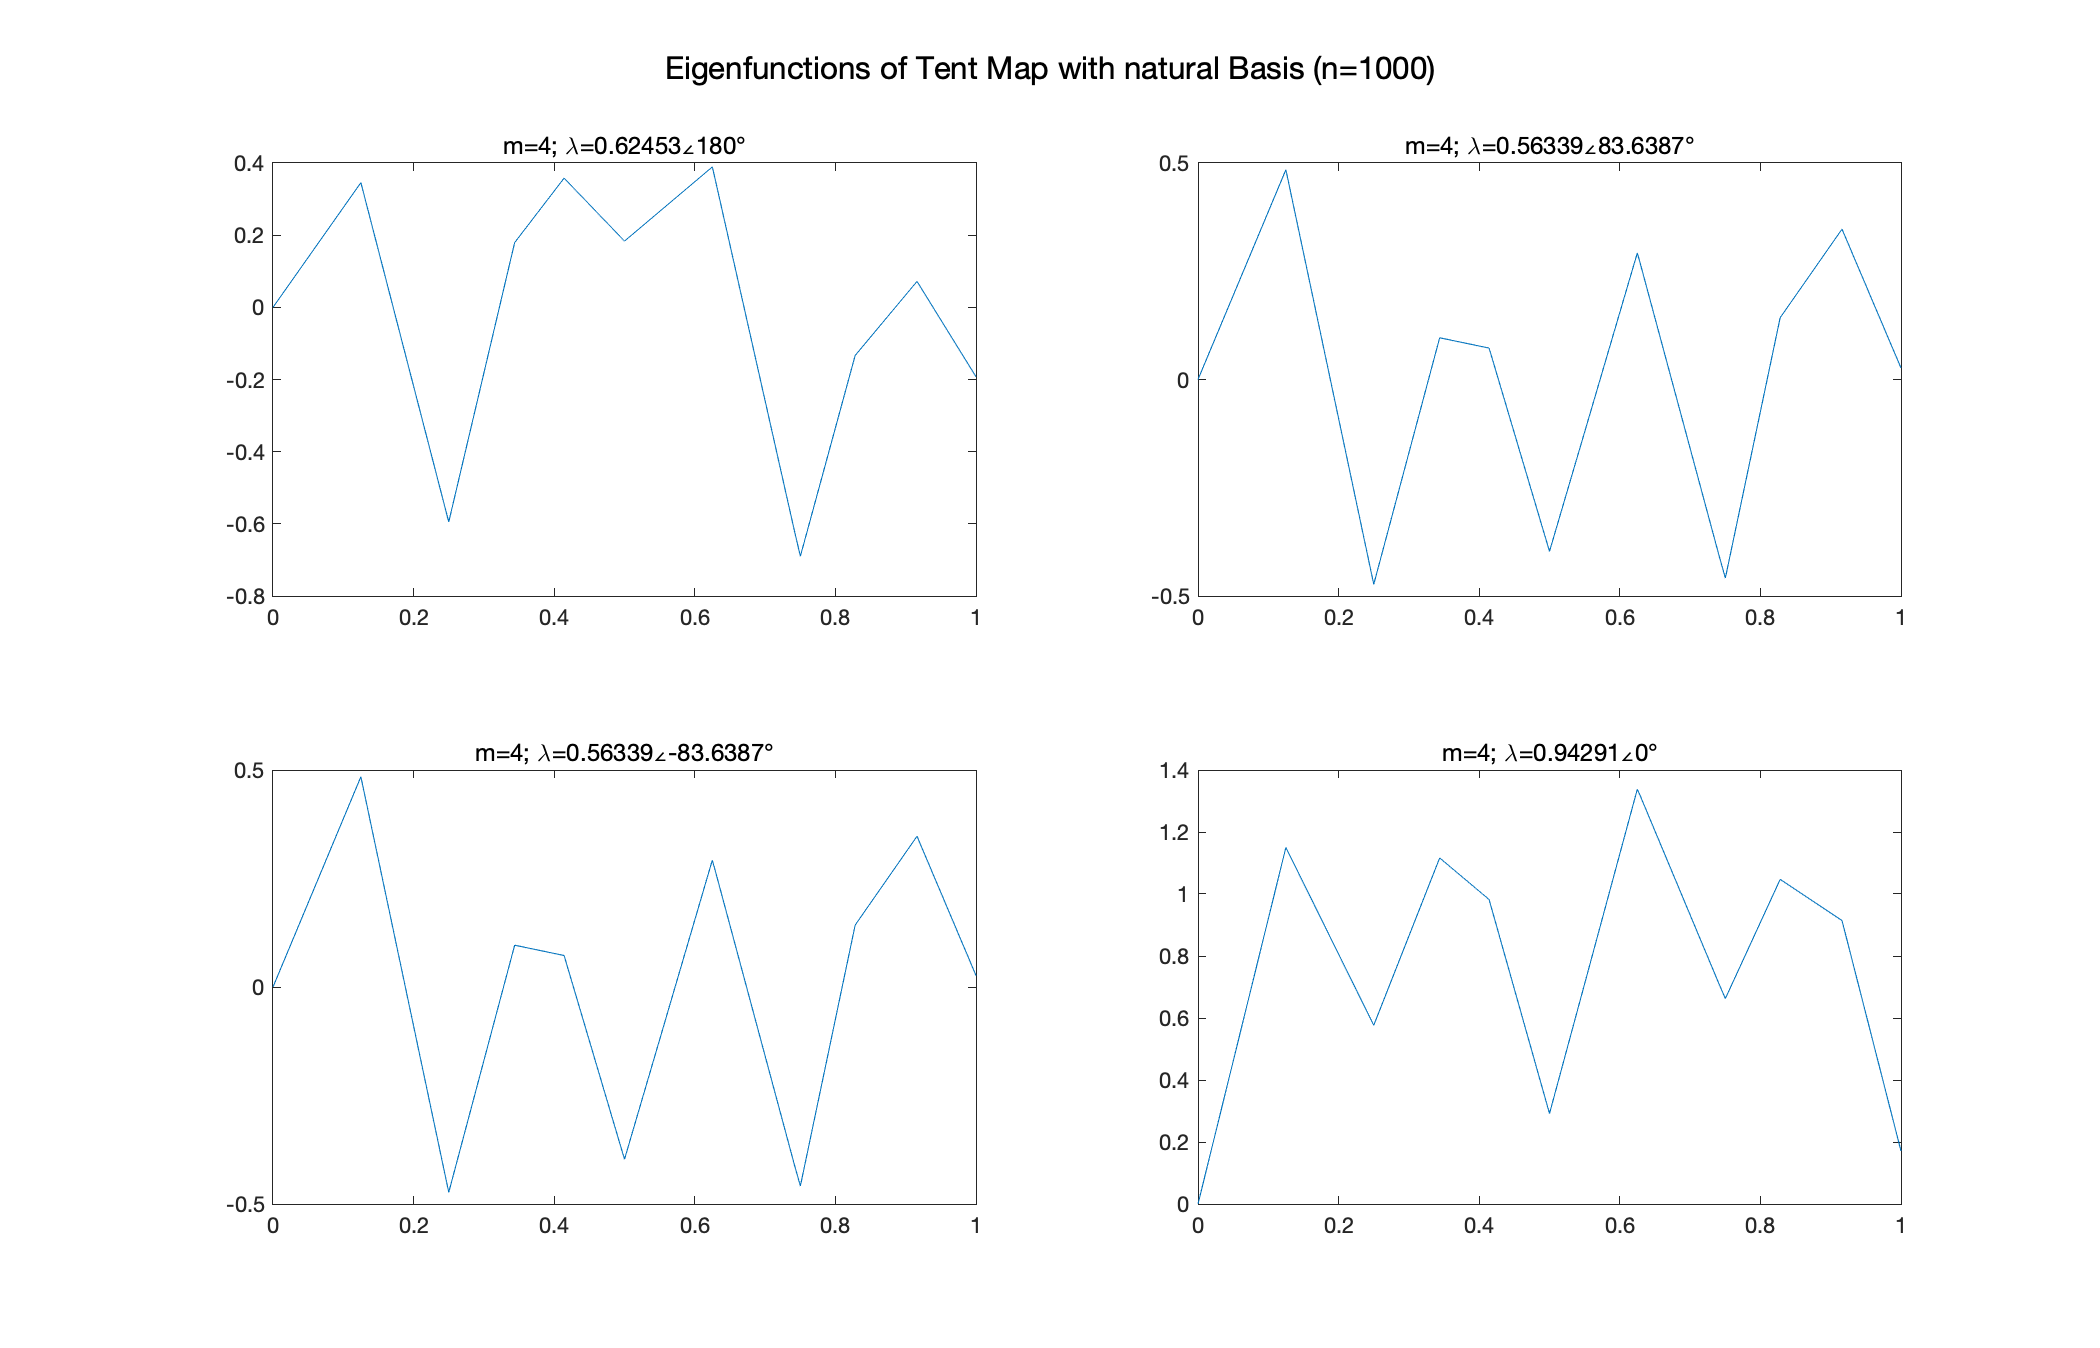
\includegraphics[scale=0.4]{tent/Tent_eigen_natural_n1000_m4}
    \caption{自然基函数下帐篷映射的本征函数($m=4$)}\label{fig:Tent_eigen_natural_n1000_m4}
\end{figure}

当我们取不同的基函数数量$m=1,2,3,4,5,6,7,8,9$且取$\lambda\approx 1$的本征函数,我们可以得到图\ref{Tent_eigen_natural_n5000_m1-2-3-4-5-6-7-8-9}。从图中我们可以发现,基函数数量每增加1,极值点出现的个数近似增加两倍。而我们又考虑到帐篷映射$T$及其多次映射$T^n$的关系:映射次数$n$每增加一次,$T^n$的相图变多增加一次弯折,即极值点的数量增加一倍。这与我们看到的本征函数图像的极值点较为相似。

\begin{figure}[!]
	\centering
	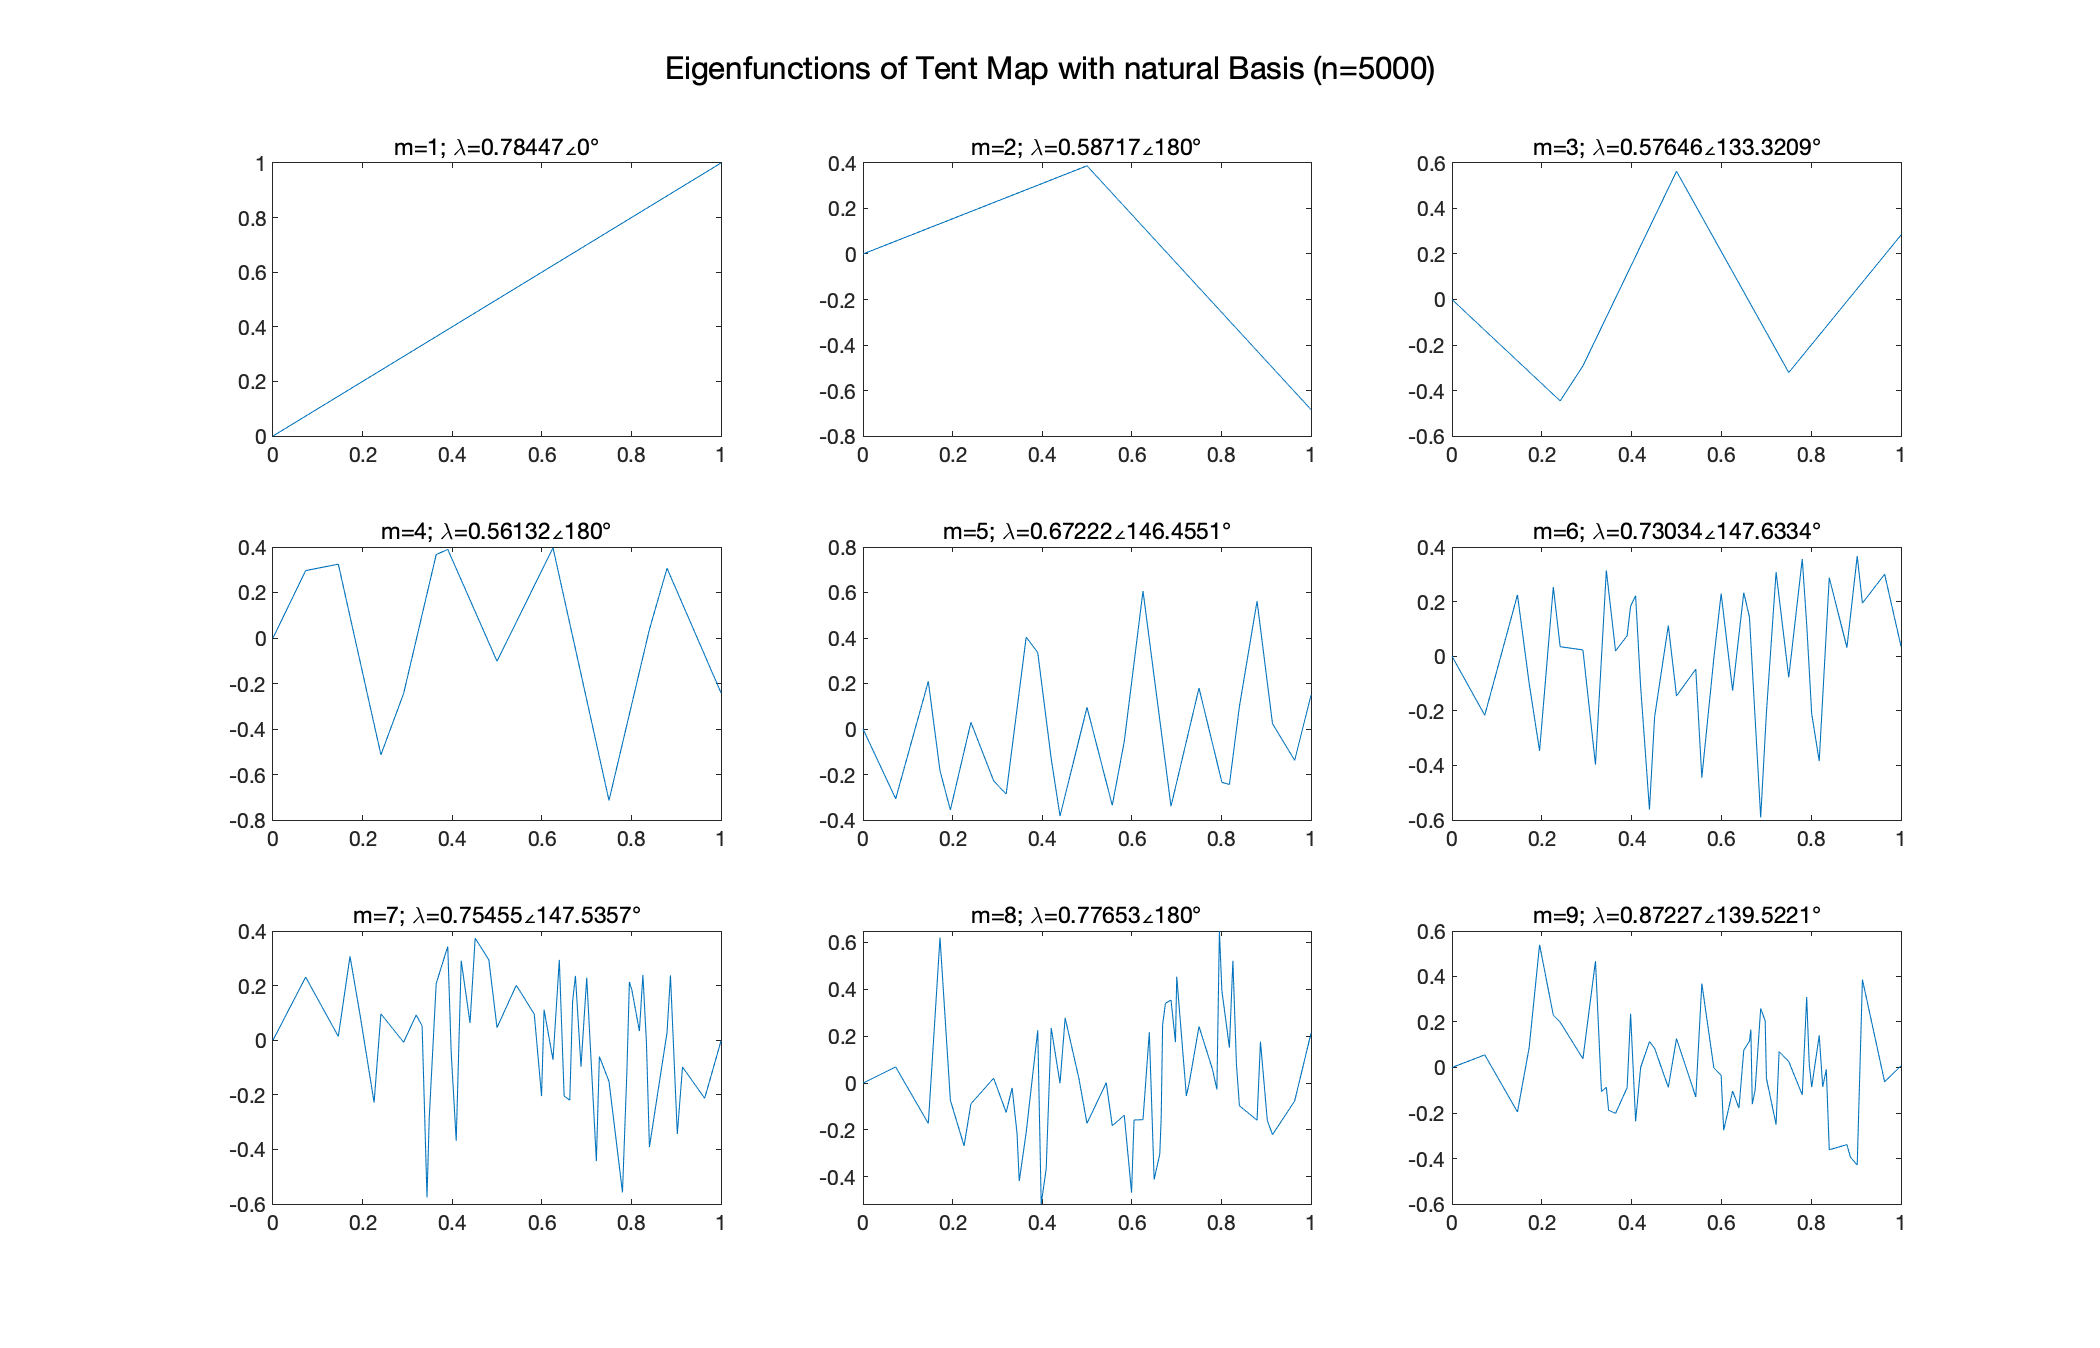
\includegraphics[scale=0.4]{tent/Tent_eigen_natural_n5000_m1-2-3-4-5-6-7-8-9}
    \caption{不同基函数数量下帐篷映射的本征函数}\label{Tent_eigen_natural_n5000_m1-2-3-4-5-6-7-8-9}
\end{figure}

无论是在正交完备基函数族还是在自然基函数中,我们都发现了在本征函数中的一些特殊的极值点,及不同基函数下本征函数之间的关系,我们将在后续的讨论中这些极值点。

\subsection{Koopman算符对帐篷映射的相空间划分}
在观察帐篷映射Kooopman算符的本征函数中我们可以发现,本征函数图像中存在一些特殊的极值点,且这些点出现的位置与我们的帐篷映射的相图有些极为相似的关系:帐篷映射中$x=\frac{1}{2}$处为映射的极值点,而$x=\frac{1}{4},\frac{3}{4}$映射一次恰到到达$x=\frac{1}{2}$处。我们考虑这些点与不动点的关系:帐篷映射存在两个不动点$x=0$和$x=\frac{2}{3}$,点$x=\frac{1}{2}$经过两次映射可以到达不动点$x=0$。我们可以将经过有限次迭代可以到达不动点处的点称之为帐篷映射的\textbf{边界点},从动力学演化的角度称之为不动点的\textbf{原像点}。我们猜测,Koopman算符的本征函数恰好就反映了这些边界点。

我们计算得到不动点$x=0$的一系列原像点,如表\ref{tab:tent_bound0}。将其按照\textbf{层次}(经过多少次演化才达到不动点)作出图像,如图\ref{fig:tent_bound0}。

\begin{table}[]
  \centering
  \begin{tabular}{|c|c|}
  \hline
  迭代次数 & 边界点($x=0$) \\ \hline
  1 & 0,\textbf{\underline{1}} \\ \hline
  2 & 0,\textbf{\underline{0.5}},1 \\ \hline
  3 & 0,\textbf{\underline{0.25}},0.5,\textbf{\underline{0.75}},1 \\ \hline
  4 & 0,\textbf{\underline{0.125}},0.25,\textbf{\underline{0.375}},0.5,\textbf{\underline{0.625}},0.75,\textbf{\underline{0.875}},1 \\ \hline
  5 & \begin{tabular}[c]{@{}l@{}}0,\textbf{\underline{0.0625}},0.125,\textbf{\underline{0.1875}},0.25,\textbf{\underline{0.3125}},0.375,\textbf{\underline{0.4375}},\\
  0.5,\textbf{\underline{0.5625}},0.625,\textbf{\underline{0.6875}},0.75,\textbf{\underline{0.8125}},0.875,\textbf{\underline{0.9375}},1\end{tabular} \\ \hline
  \end{tabular}
  \caption[帐篷映射的边界点($x=0$)]{帐篷映射的边界点($x=0$):经过多少次迭代可以到达不动点$x=0$,下划线的点是每层次的新增点}\label{tab:tent_bound0}
\end{table}

\begin{figure}[!]
	\centering
	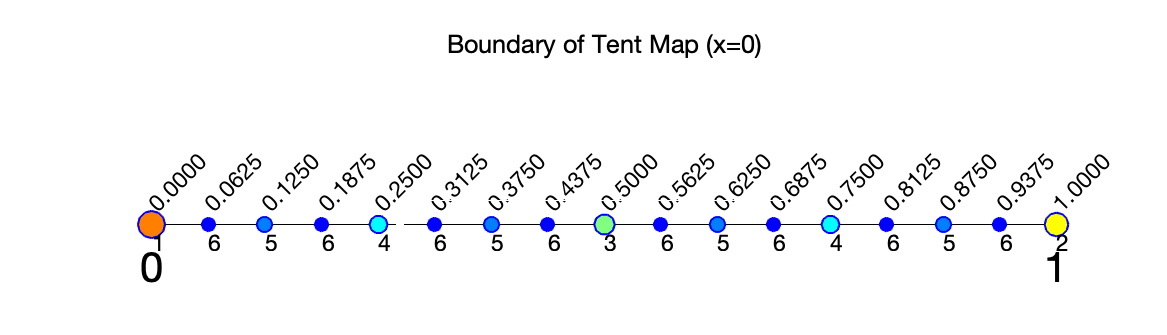
\includegraphics[scale=0.6]{tent/Tent_boundarys_x0}
    \caption[帐篷映射的边界点($x=0$)]{帐篷映射的边界点($x=0$):相同大小和颜色的点同属于一个层次}\label{fig:tent_bound0}
\end{figure}

同样,对于另一个不动点$x=\frac{2}{3}$,我们同样作出其一系列原像点(表\ref{tab:tent_bound2-3}),且按层次绘制其在相空间的位置(图\ref{fig:tent_bound2-3})。

\begin{table}[]
  \centering
  \begin{tabular}{|c|c|}
  \hline
  迭代次数 & 边界点($x=\frac{2}{3}$) \\ \hline
  0 & 0.6666 \\ \hline
  1 & \textbf{\underline{0.3333}},0.6666 \\ \hline
  2 & \textbf{\underline{0.1666}},0.3333,0.6666,\textbf{\underline{0.8333}} \\ \hline
  3 & \textbf{\underline{0.0833}},0.1666,0.3333,\textbf{\underline{0.4166}},\textbf{\underline{0.5833}},0.6666,0.8333,\textbf{\underline{0.9166}} \\ \hline
  4 & \begin{tabular}[c]{@{}l@{}}\textbf{\underline{0.04166}},0.0833,0.1666,\textbf{\underline{0.2083}},\textbf{\underline{0.2916}},0.3333,0.4166,\textbf{\underline{0.4583}},\\ \textbf{\underline{0.5416}},0.5833,0.6666,\textbf{\underline{0.7083}},\textbf{\underline{0.7916}},0.8333,0.9166,\textbf{\underline{0.9583}}\end{tabular} \\ \hline
  \end{tabular}
  \caption[帐篷映射的边界点($x=\frac{2}{3}$)]{帐篷映射的边界点($x=\frac{2}{3}$):经过多少次迭代可以到达不动点$x=\frac{2}{3}$,下划线的点是每层次的新增点}\label{tab:tent_bound2-3}
\end{table}
\begin{figure}[!]
	\centering
	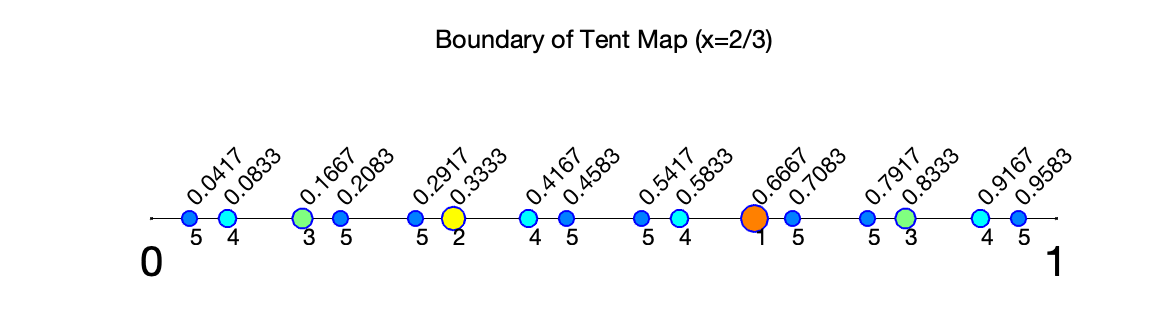
\includegraphics[scale=0.6]{tent/Tent_boundarys_x2-3}
    \caption[帐篷映射的边界点($x=\frac{2}{3}$)]{帐篷映射的边界点($x=\frac{2}{3}$):相同大小和颜色的点同属于一个层次}\label{fig:tent_bound2-3}
\end{figure}

观察这些边界点的位置,对比我们之前观察到本征函数的极值点,更加印证了我们之前的猜想:Koopman算符的本征函数反映了边界点的划分。为了证实我们的猜测,我们将本征函数和边界点的位置进行对比观察:在图\ref{fig:Tent_eigen_noise_n1000m2d0}中,我们取不同的基函数数量$m=2,3,4,5,8,10,15,20$,并绘制最多9个本征函数图像,将本征函数图像的极值点标出,并将帐篷映射的边界点同时标出,以此来对比二者之间的关系。

\begin{figure}[!]
  \centering%[2,3,4,5,8,10,15,20]
  \subfloat[m=2]{
    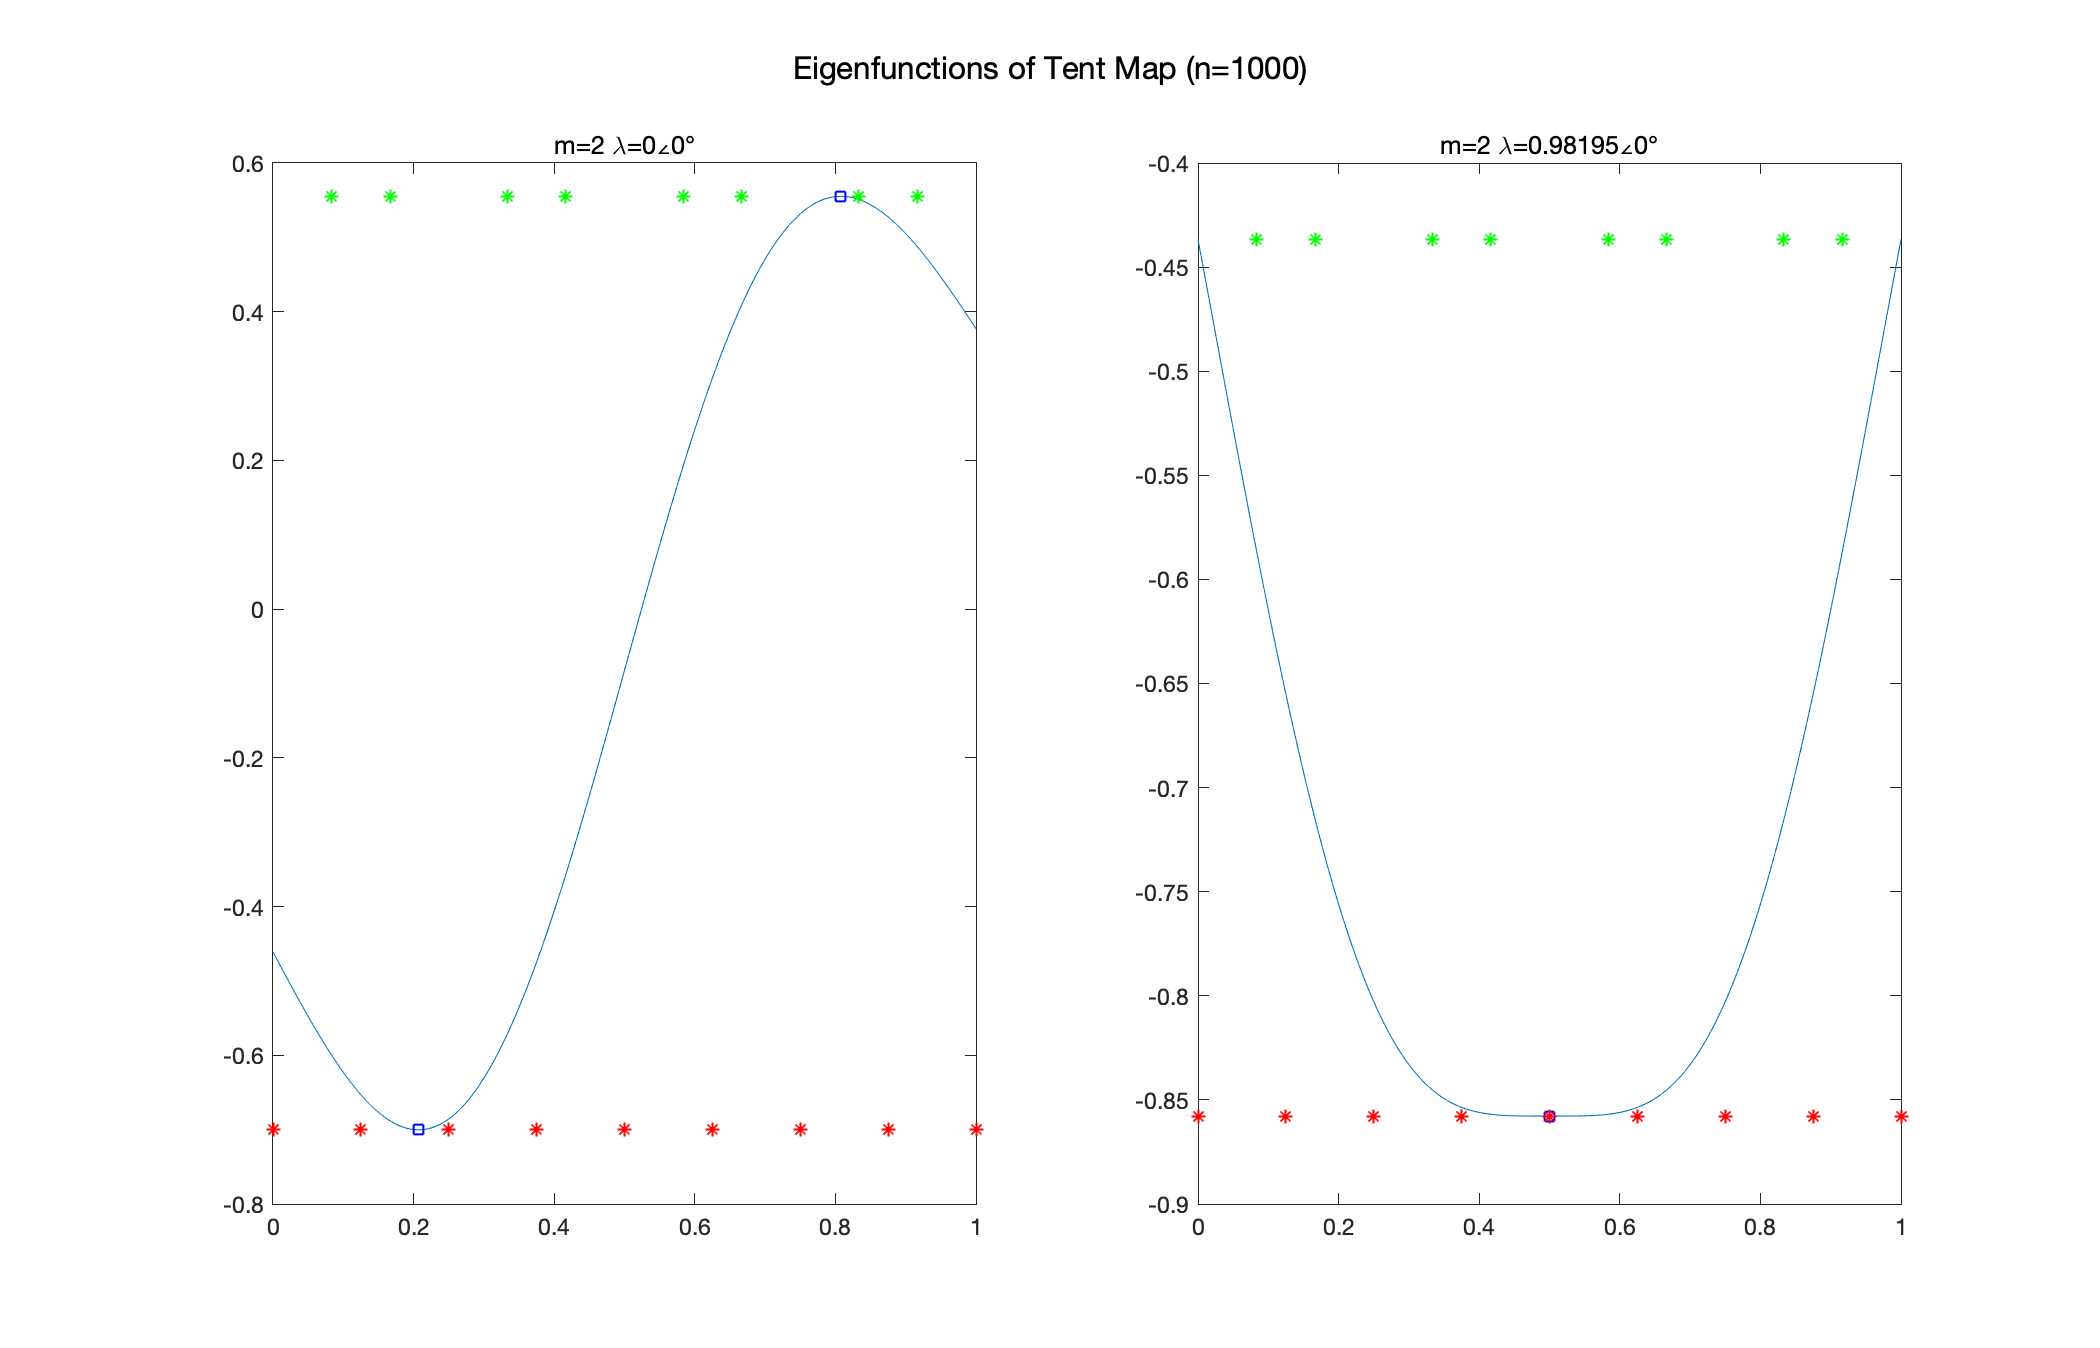
\includegraphics[scale=0.2]{tent/noise/Tent_eigen_noise_n1000m2d0}}
  \subfloat[m=3]{
    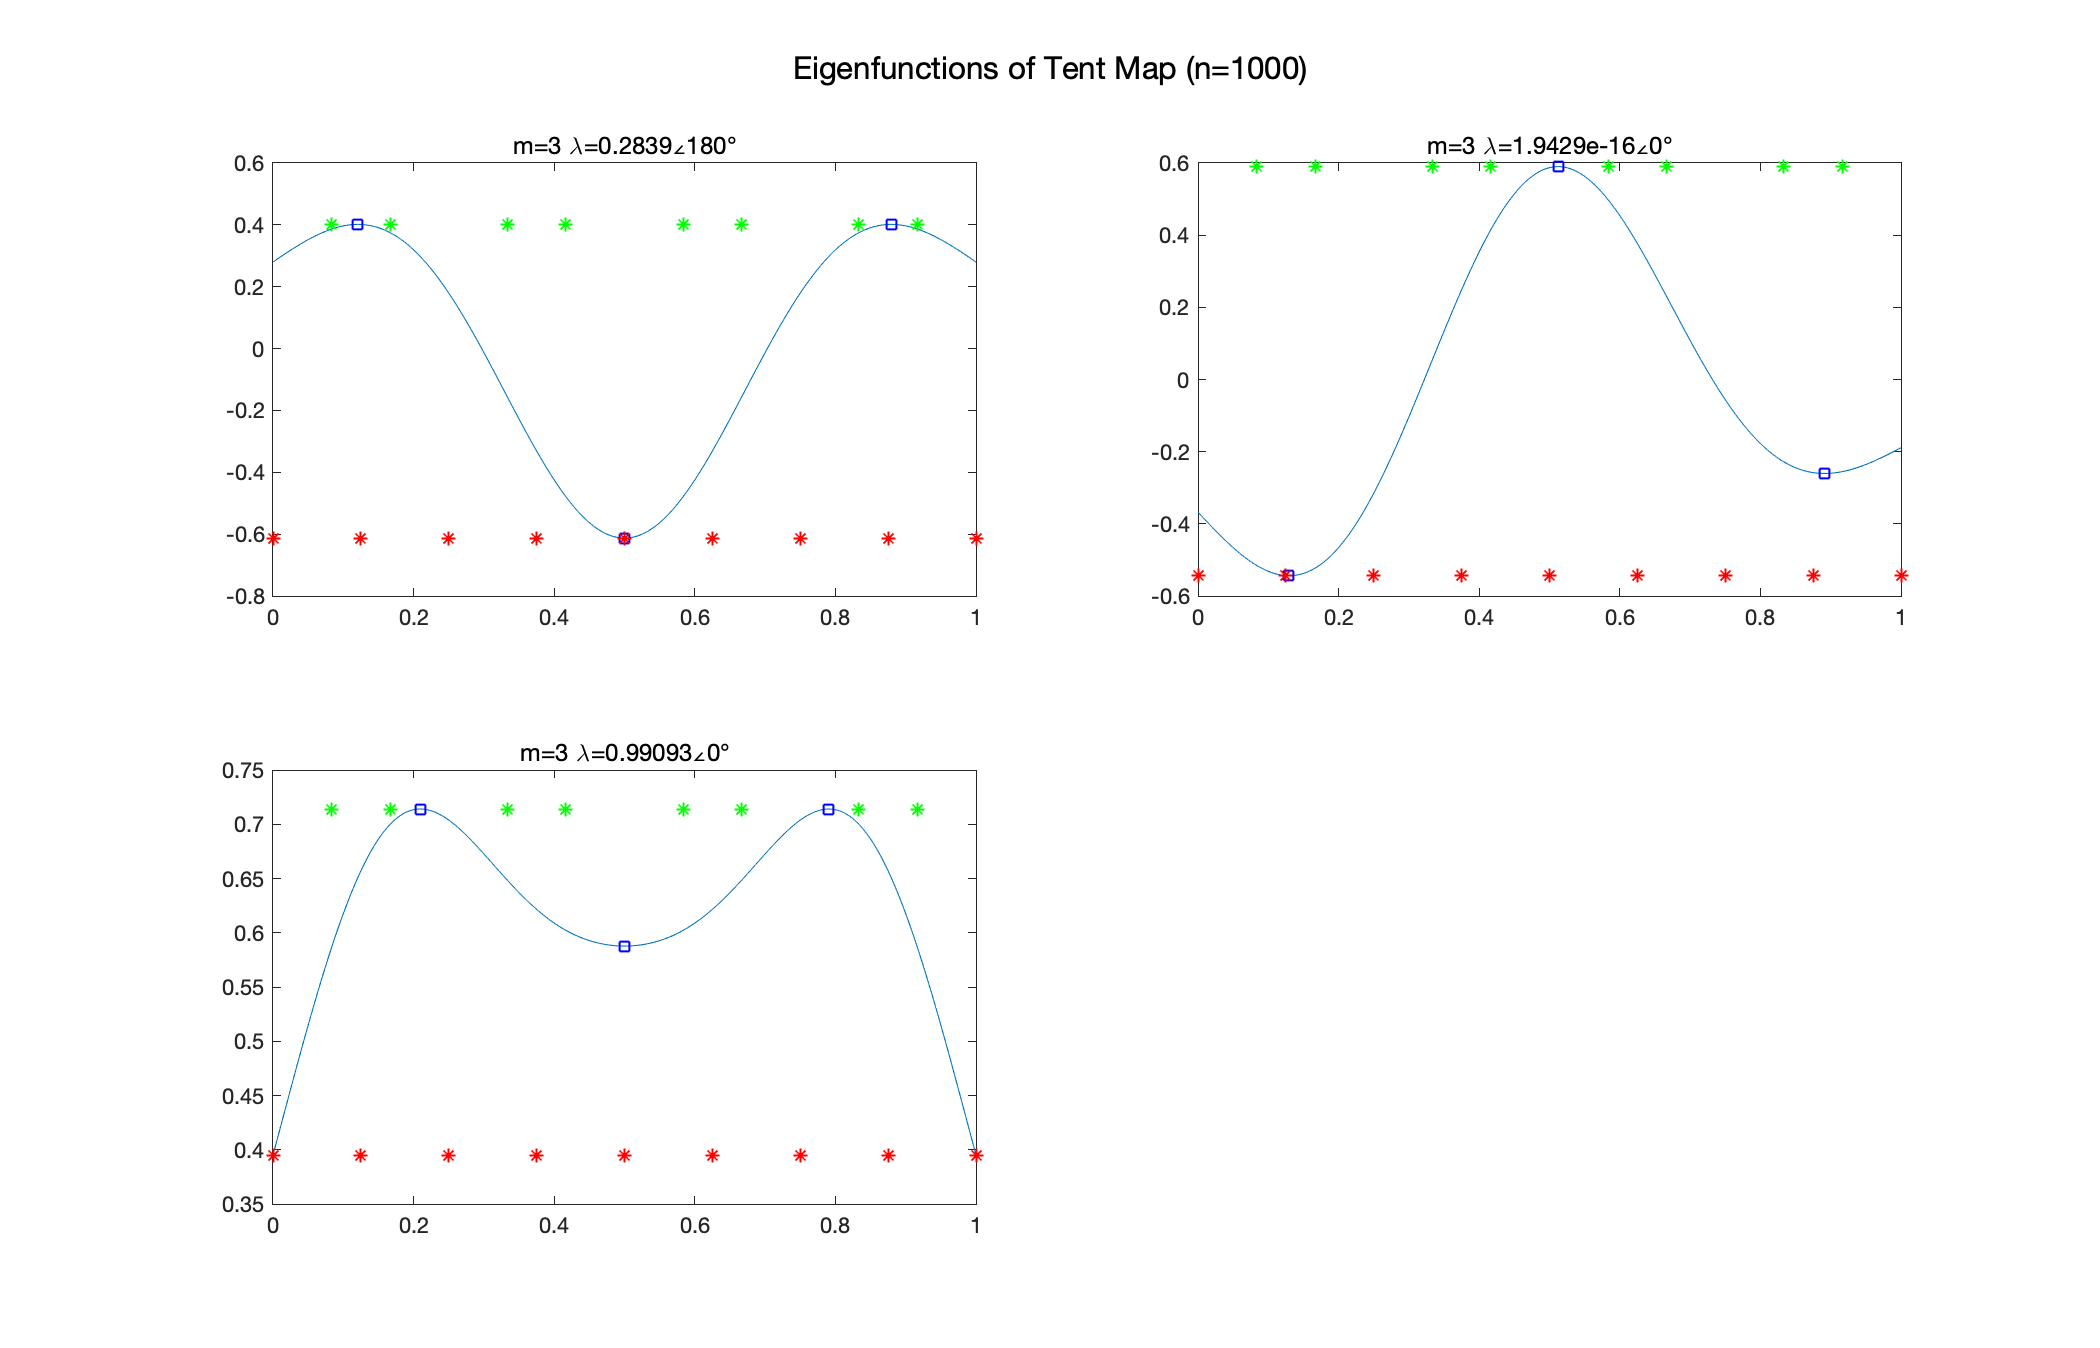
\includegraphics[scale=0.2]{tent/noise/Tent_eigen_noise_n1000m3d0}}
    \\
  \subfloat[m=4]{
    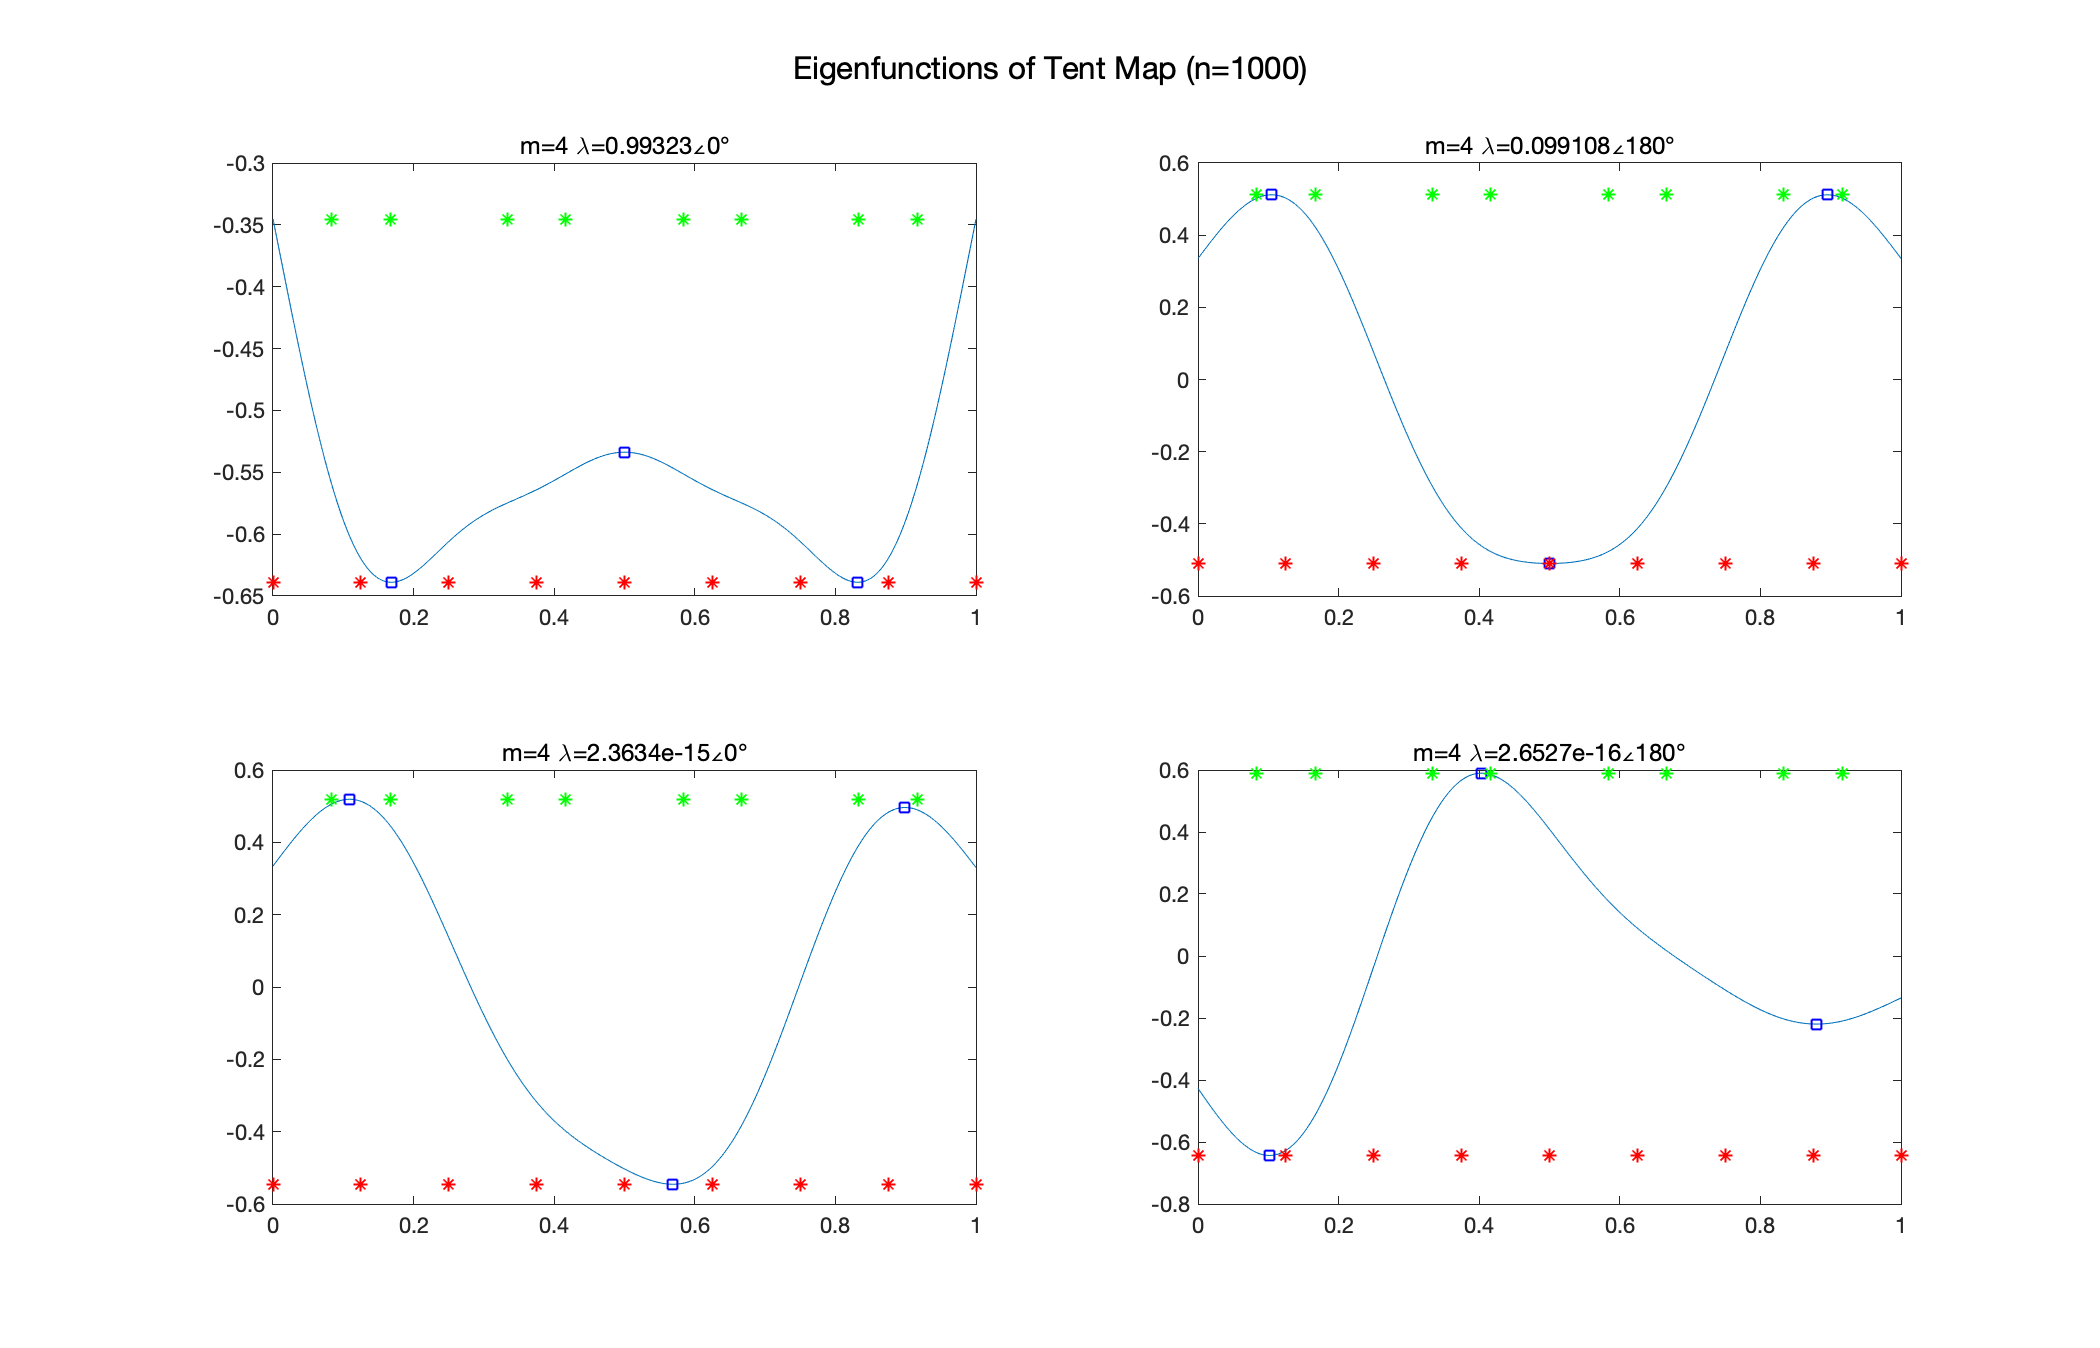
\includegraphics[scale=0.2]{tent/noise/Tent_eigen_noise_n1000m4d0}}
  \subfloat[m=5]{
    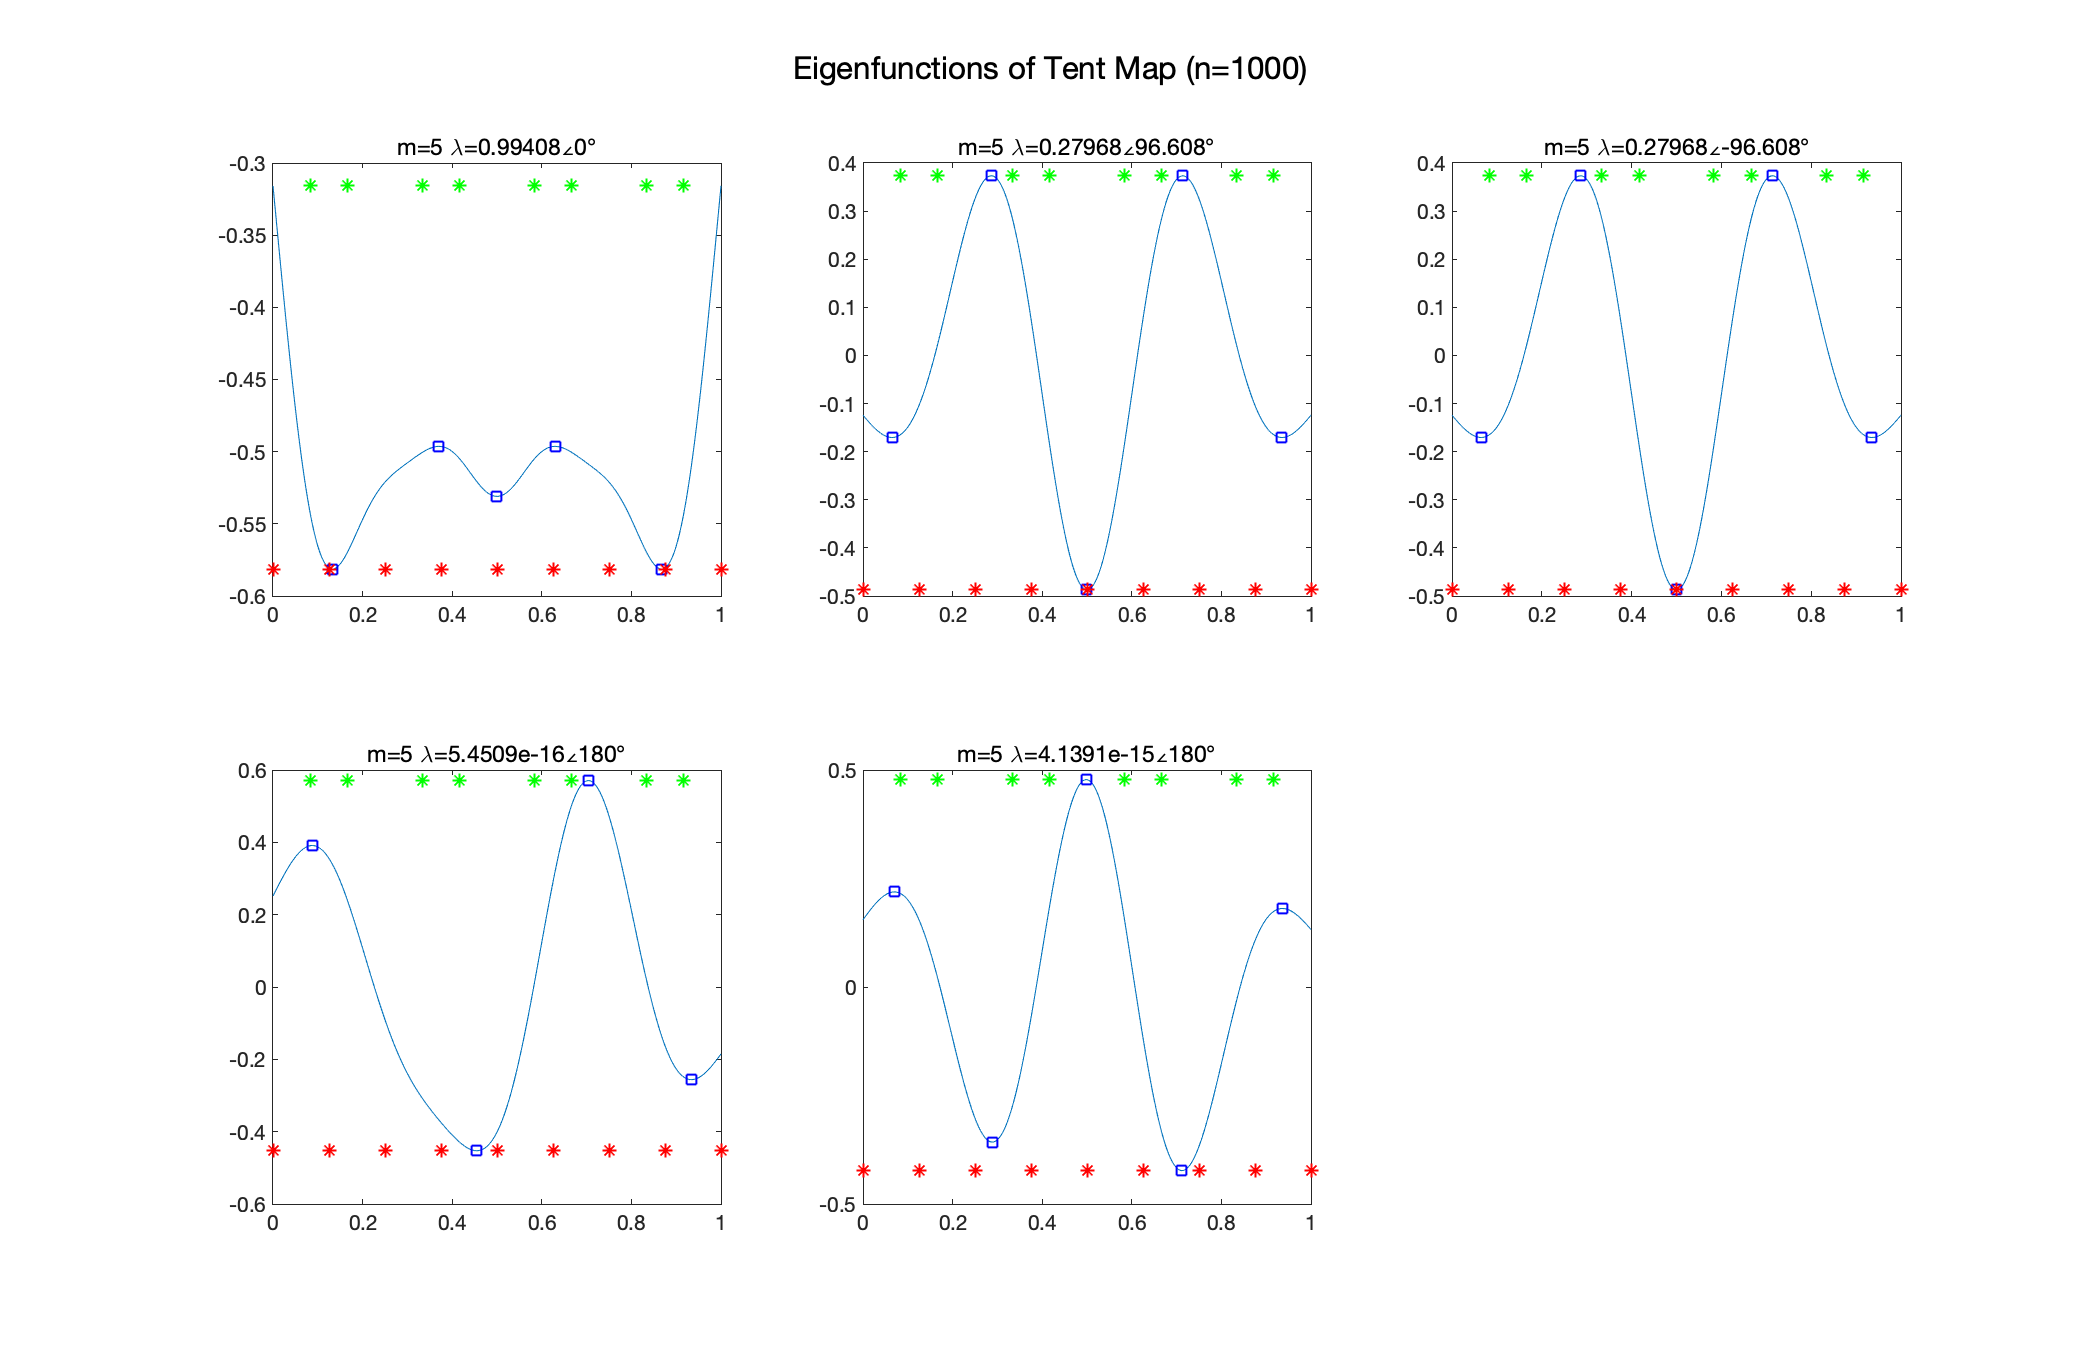
\includegraphics[scale=0.2]{tent/noise/Tent_eigen_noise_n1000m5d0}}
    \\
  \subfloat[m=8]{
    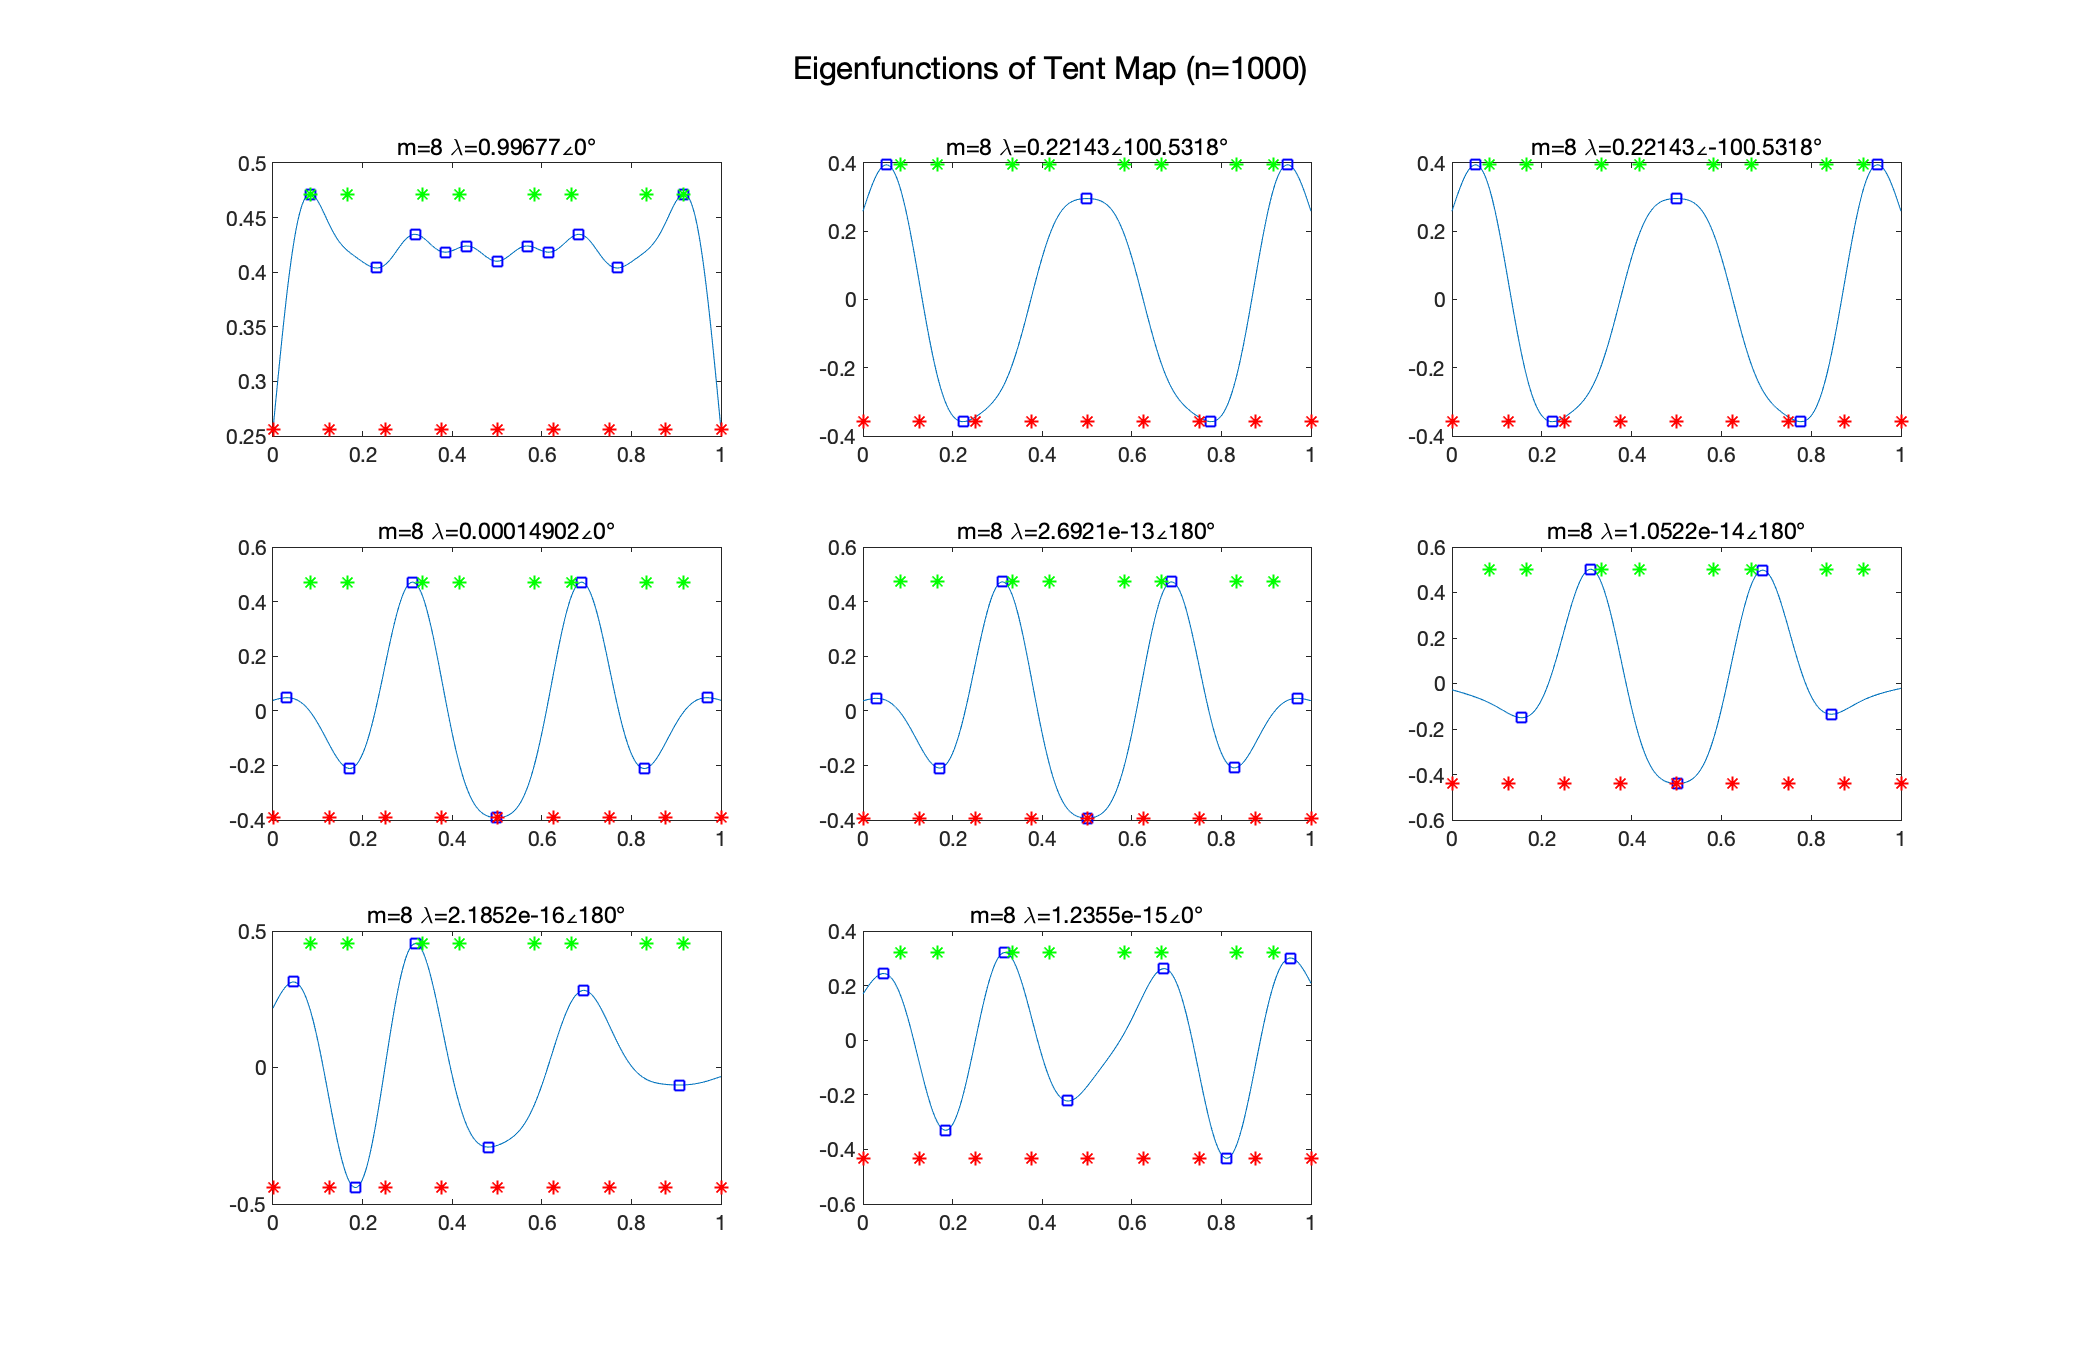
\includegraphics[scale=0.2]{tent/noise/Tent_eigen_noise_n1000m8d0}}
  \subfloat[m=10]{
    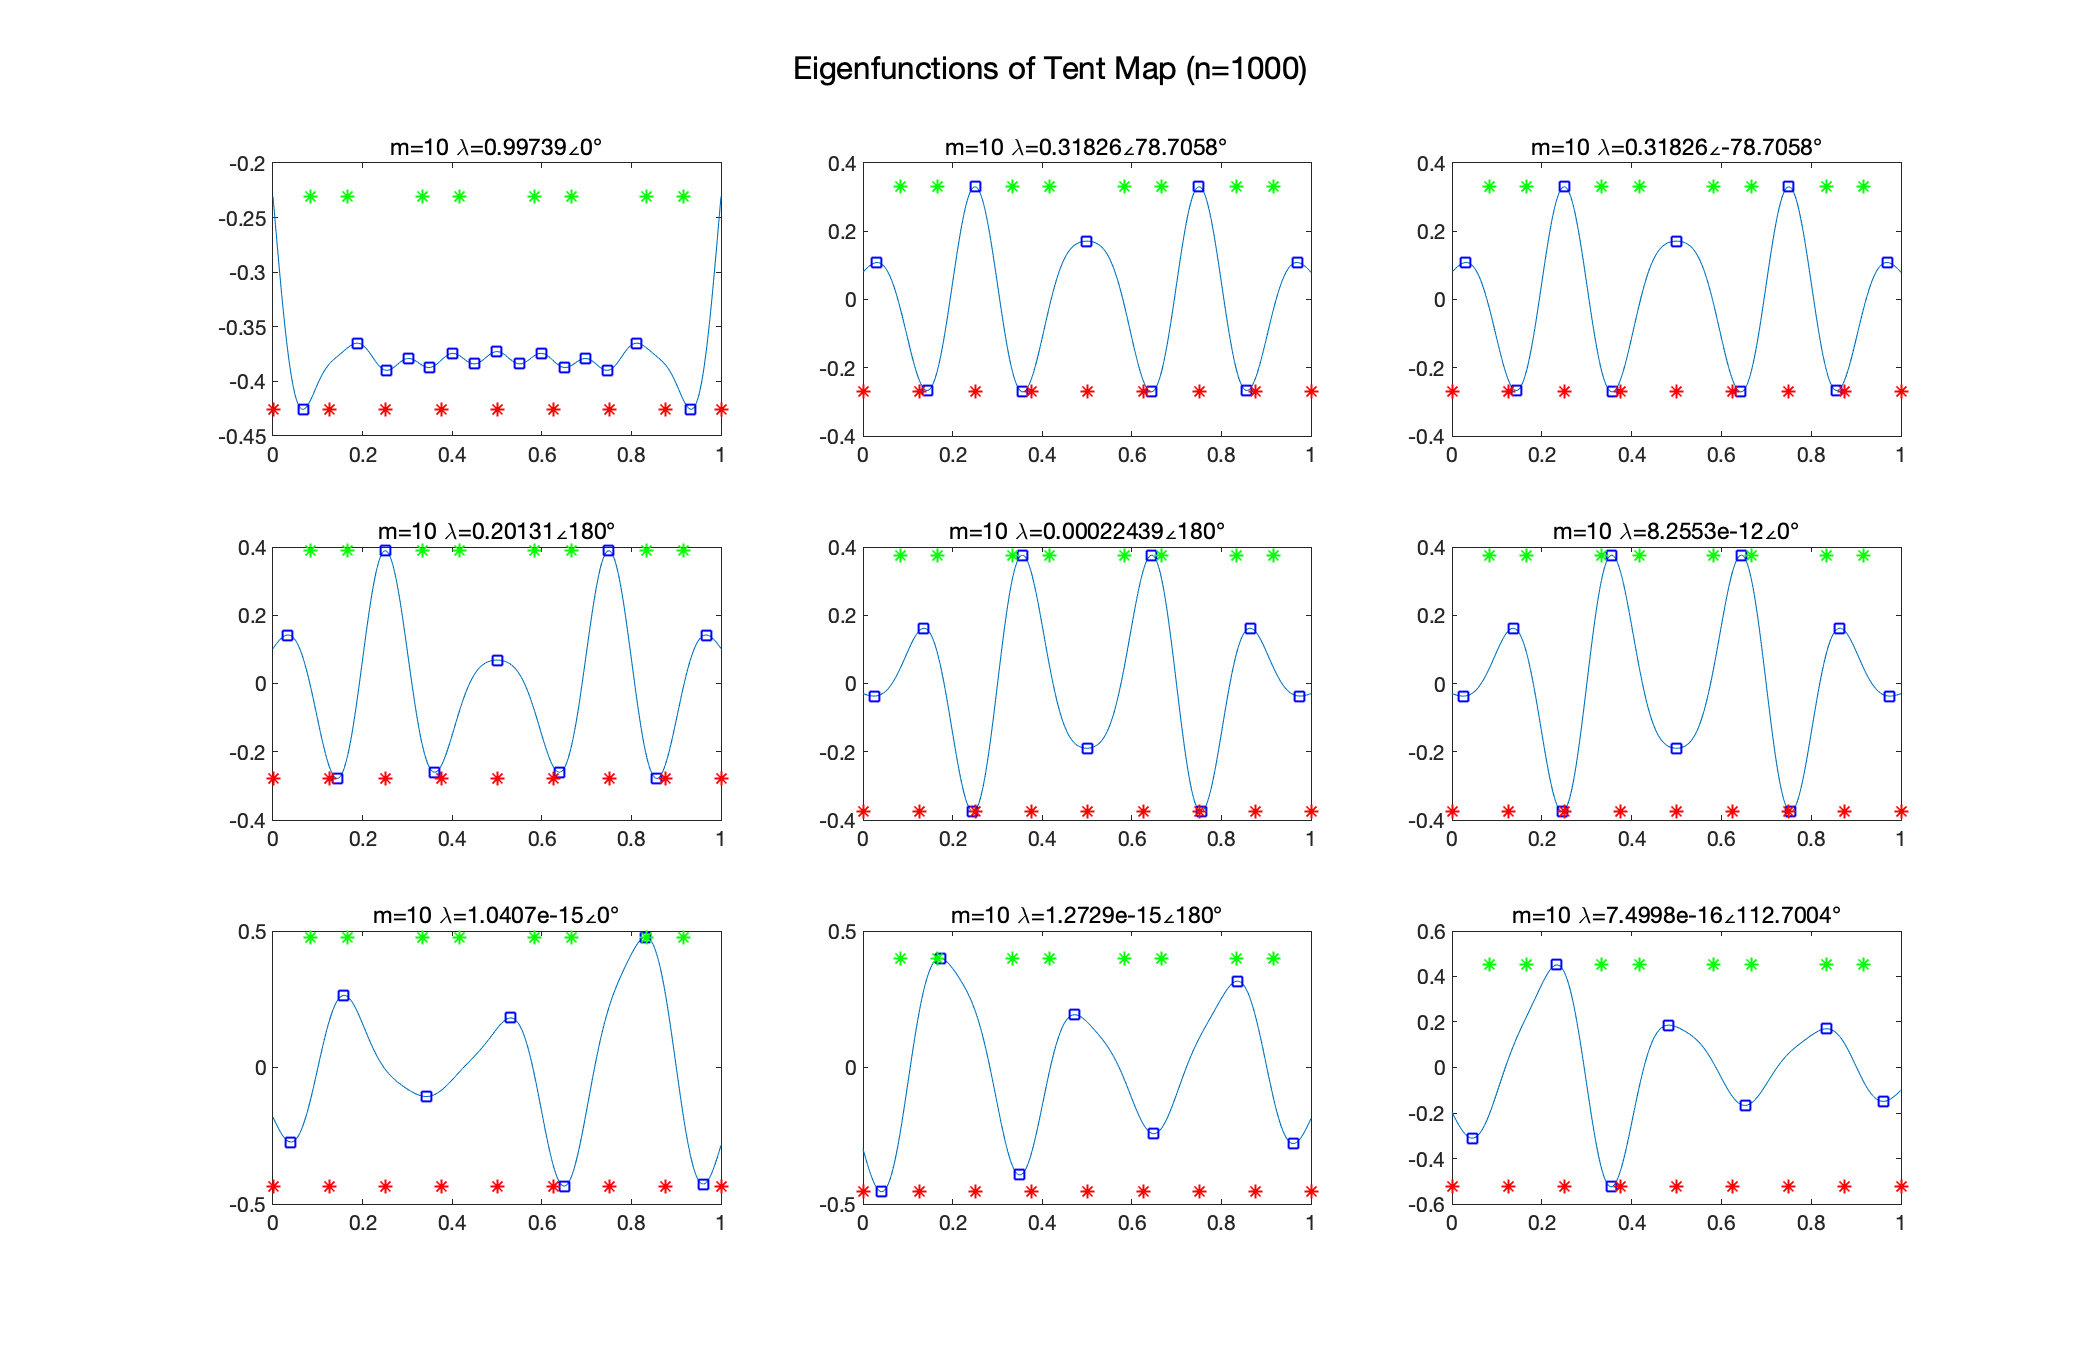
\includegraphics[scale=0.2]{tent/noise/Tent_eigen_noise_n1000m10d0}}
    \\
  \subfloat[m=15]{
    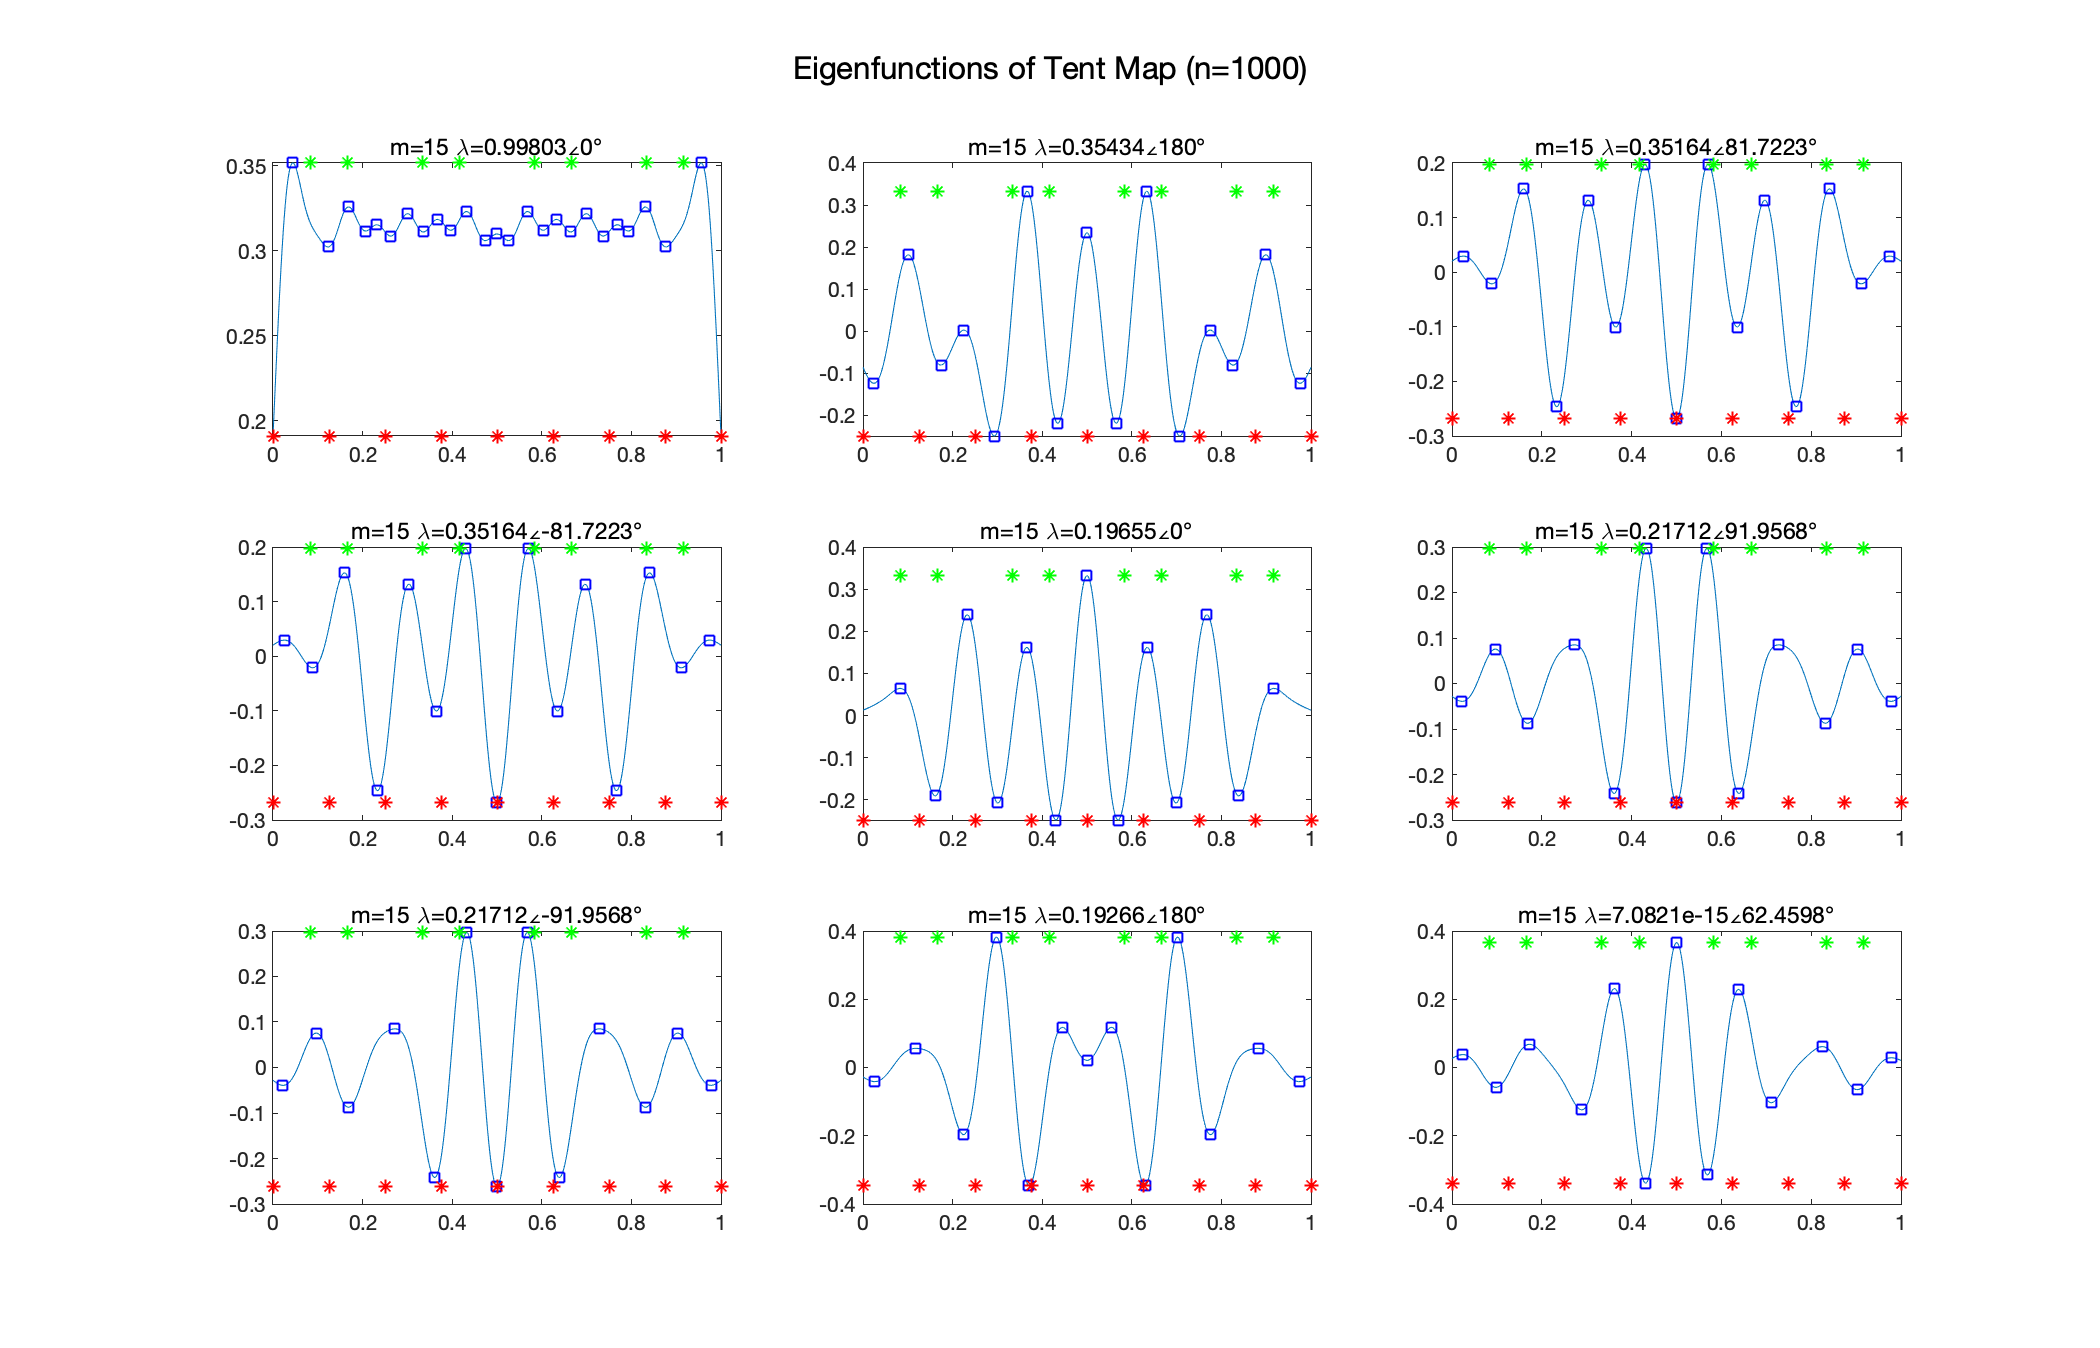
\includegraphics[scale=0.2]{tent/noise/Tent_eigen_noise_n1000m15d0}}
  \subfloat[m=20]{
    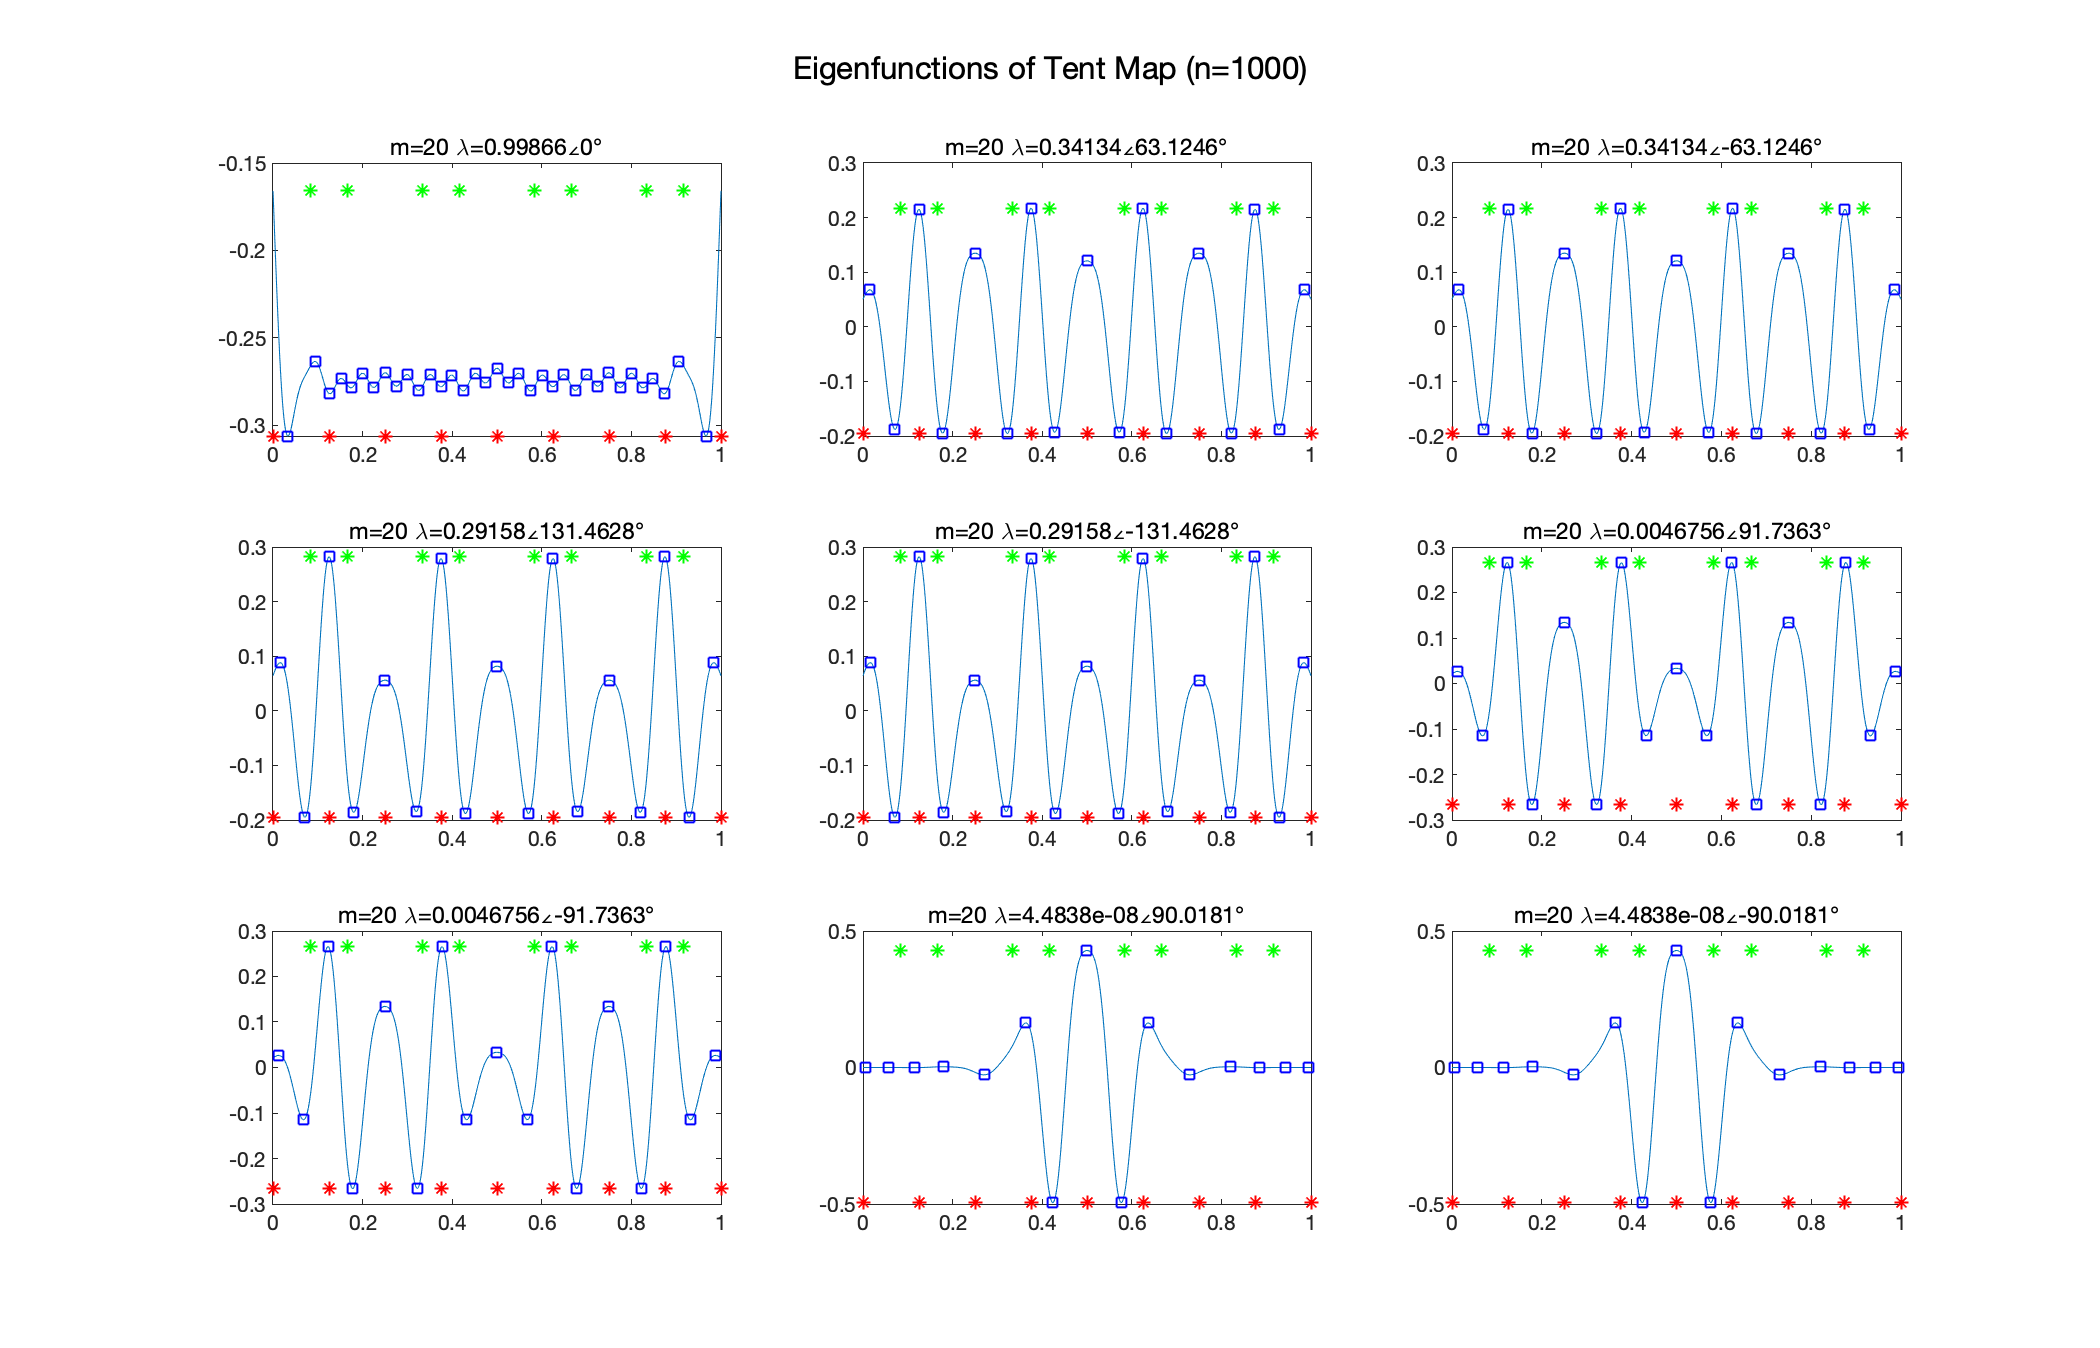
\includegraphics[scale=0.2]{tent/noise/Tent_eigen_noise_n1000m20d0}}
    \\
  \caption[帐篷映射的边界点与本征函数]{帐篷映射的边界点与本征函数:每个图中红色的点为$x=0$系列的边界点,绿色的点为$x=\frac{2}{3}$系列的边界点(不区分层次),且本征函数的极值点用空心方块标出}\label{fig:Tent_eigen_noise_n1000m2d0}
\end{figure}

我们观察本征函数的极值点与帐篷映射的边界点,在图\ref{fig:Tent_eigen_noise_n1000m2d0}(a)的第二个小图中,我们观察到基函数$m=2$时本征函数存在一个极值点,其与边界点$x=\frac{1}{2}$是比较吻合的。在图\ref{fig:Tent_eigen_noise_n1000m2d0}(b)中,基函数数量$m=3$,由于高斯基函数格点数量有限,其不可能在$x=\frac{1}{4},\frac{3}{4}$处有极值点,但观察图像我们发现其在这些点的附近出现了极值点。随着基函数数量的增加$m=4,5,8,10$时,$x=\frac{1}{4},\frac{3}{4}$处附近的极值点越来越逼近这两个边界点,当$m=15$时,$x=\frac{1}{4},\frac{3}{4}$处附近各存在一个极值点;当$m=20$时,极值点与边界点吻合的较好。

我们可以得出初步结论:Koopman算符的本征函数的极值点确实反映了帐篷映射的边界点,且随着本征函数基函数数量的增加,函数格点的增加使本征函数的精细度增加,从而能更精确的刻画帐篷映射的边界点。这些边界点即对应着我们对相空间的划分:我们可以依本征函数的极值点对相空间区域进行划分。在上一章的讨论中我们了解到,这些帐篷映射的边界点其实就是符号动力学的分界点,这为我们提供了一种寻找符号动力学分界点的方法:Koopman算符的本征函数极值点可以反映符号动力学的分界点,若其能成为一个普遍的规律,当我们面对一个较复杂的系统时,我们可以通过Koopman算符的本征函数寻找其极值点,来寻找该系统对应的符号动力学的分界点。且随着我们增加基函数的数量,我们便能更精细的刻画符号动力学的分界点。从而使我们对该动力学的特征能够有着粗粒度的认识。

\subsection{更多的讨论}
我们有了初步的结论:Koopman算符的本征函数的极值点反映了帐篷映射的边界点。然而我们需要对这个结论作进一步的探究,我们可以提出以下三个问题:
\begin{itemize}
\item 这个结论是否具有鲁棒性?
\item 这种方法寻找到的边界点准确吗?若不够精确如何提高精确度?
\item 这种寻找边界点的方法适用于其他系统吗?
\end{itemize}
我们将针对以上三个问题,进一步讨论Koopman算符的本征函数及其对帐篷映射边界点的划分。

\subsubsection{噪声对Koopman算符的影响}
在现实系统中,动力学系统的演化都会受到涨落的影响,即每次的演化都会有一定的浮动,若Koopman算符不具有鲁棒性,则为寻找边界点带来了一定的困难,为此我们假设我们的涨落符合高斯白噪声分布,将帐篷映射加入噪声项:
\begin{equation}
  x_{n+1}=f(x_n)=1-2|x_n-\frac{1}{2}|+\xi
\end{equation}
其中高斯分布的方差作为信噪比的参数可供调节,帐篷映射在不同噪声大小下的相图如图\ref{fig:Tent_noise_phase_d0}所示。若Koopman算符对边界点的划分具有鲁棒性,则在此噪声影响下,Koopman算符对边界点的划分应与之前相差无几。

\begin{figure}[!]
  \centering
  \subfloat[noise=0]{
    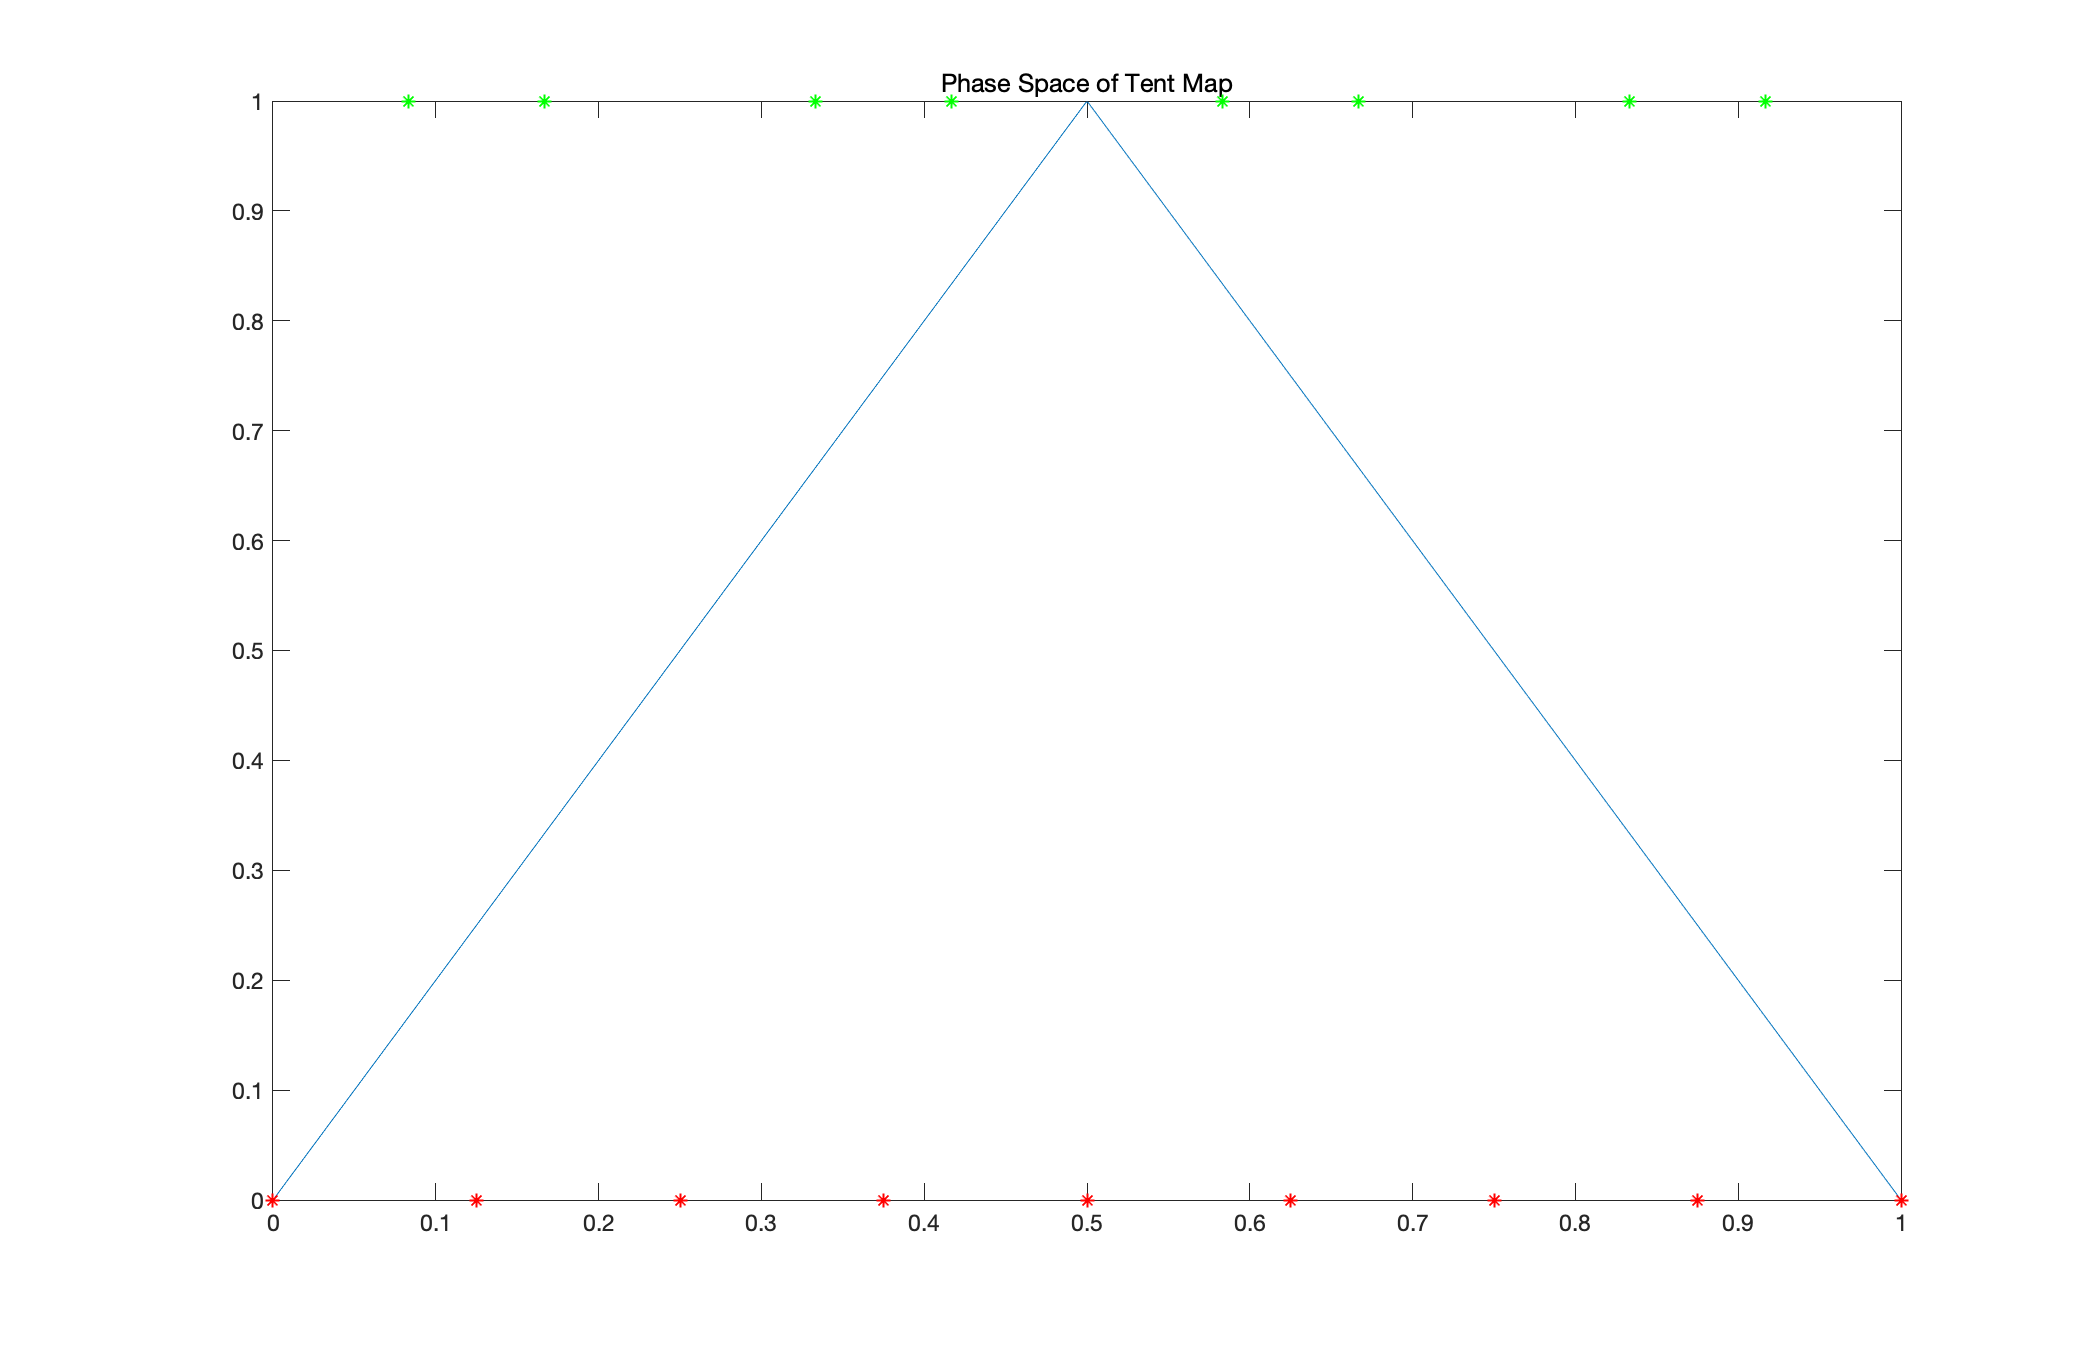
\includegraphics[scale=0.13]{tent/noise/Tent_noise_phase_d0}}
  \subfloat[noise=0.001]{
    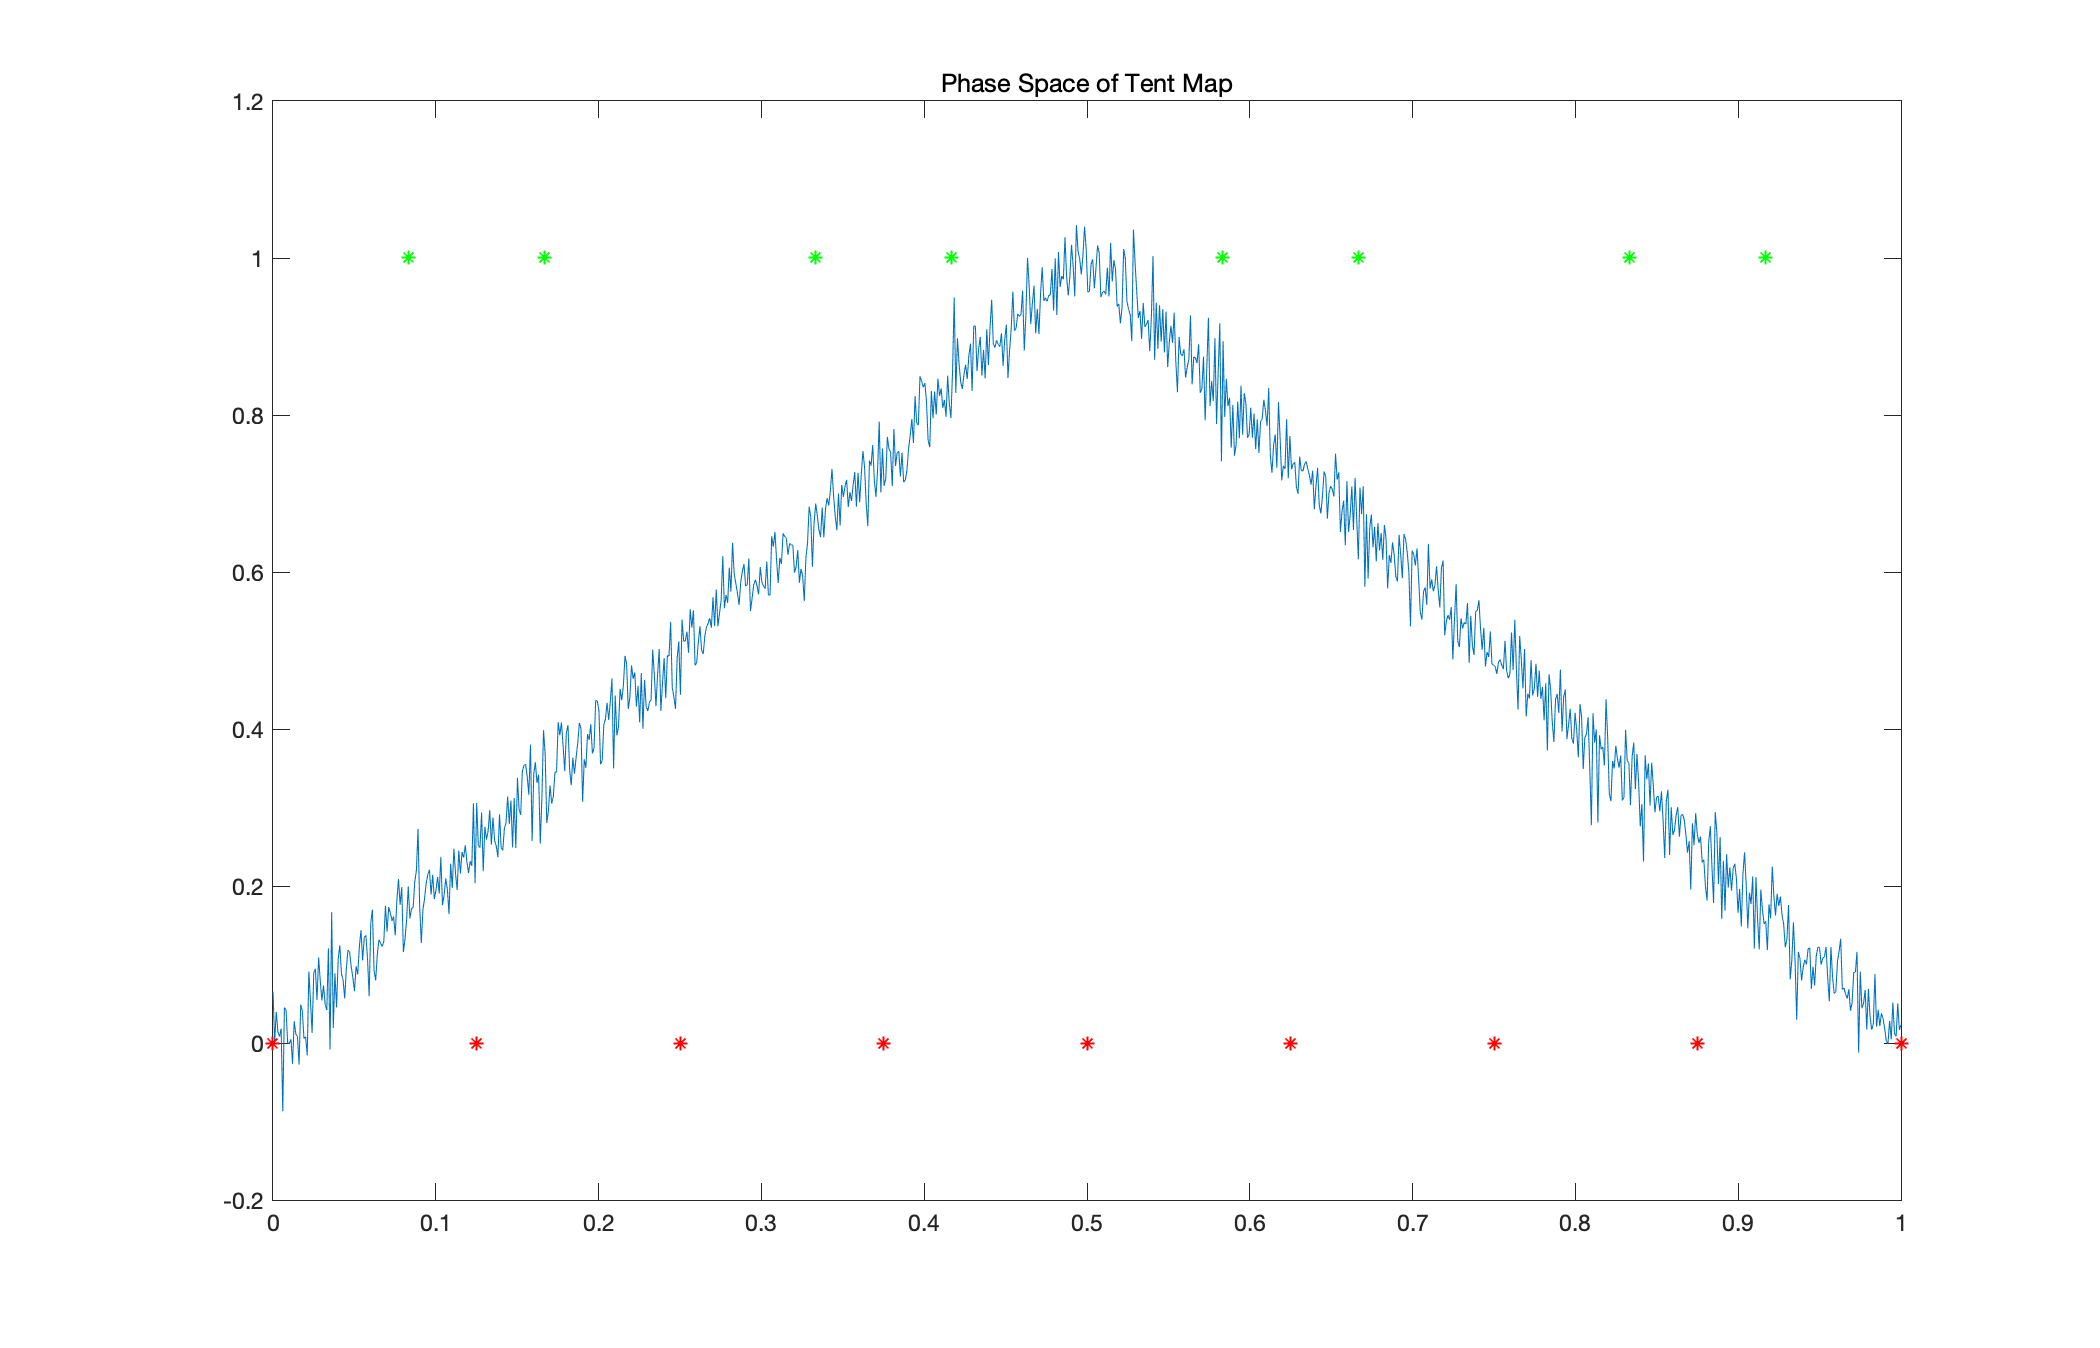
\includegraphics[scale=0.13]{tent/noise/Tent_noise_phase_d0-001}}
  \subfloat[noise=0.01]{
    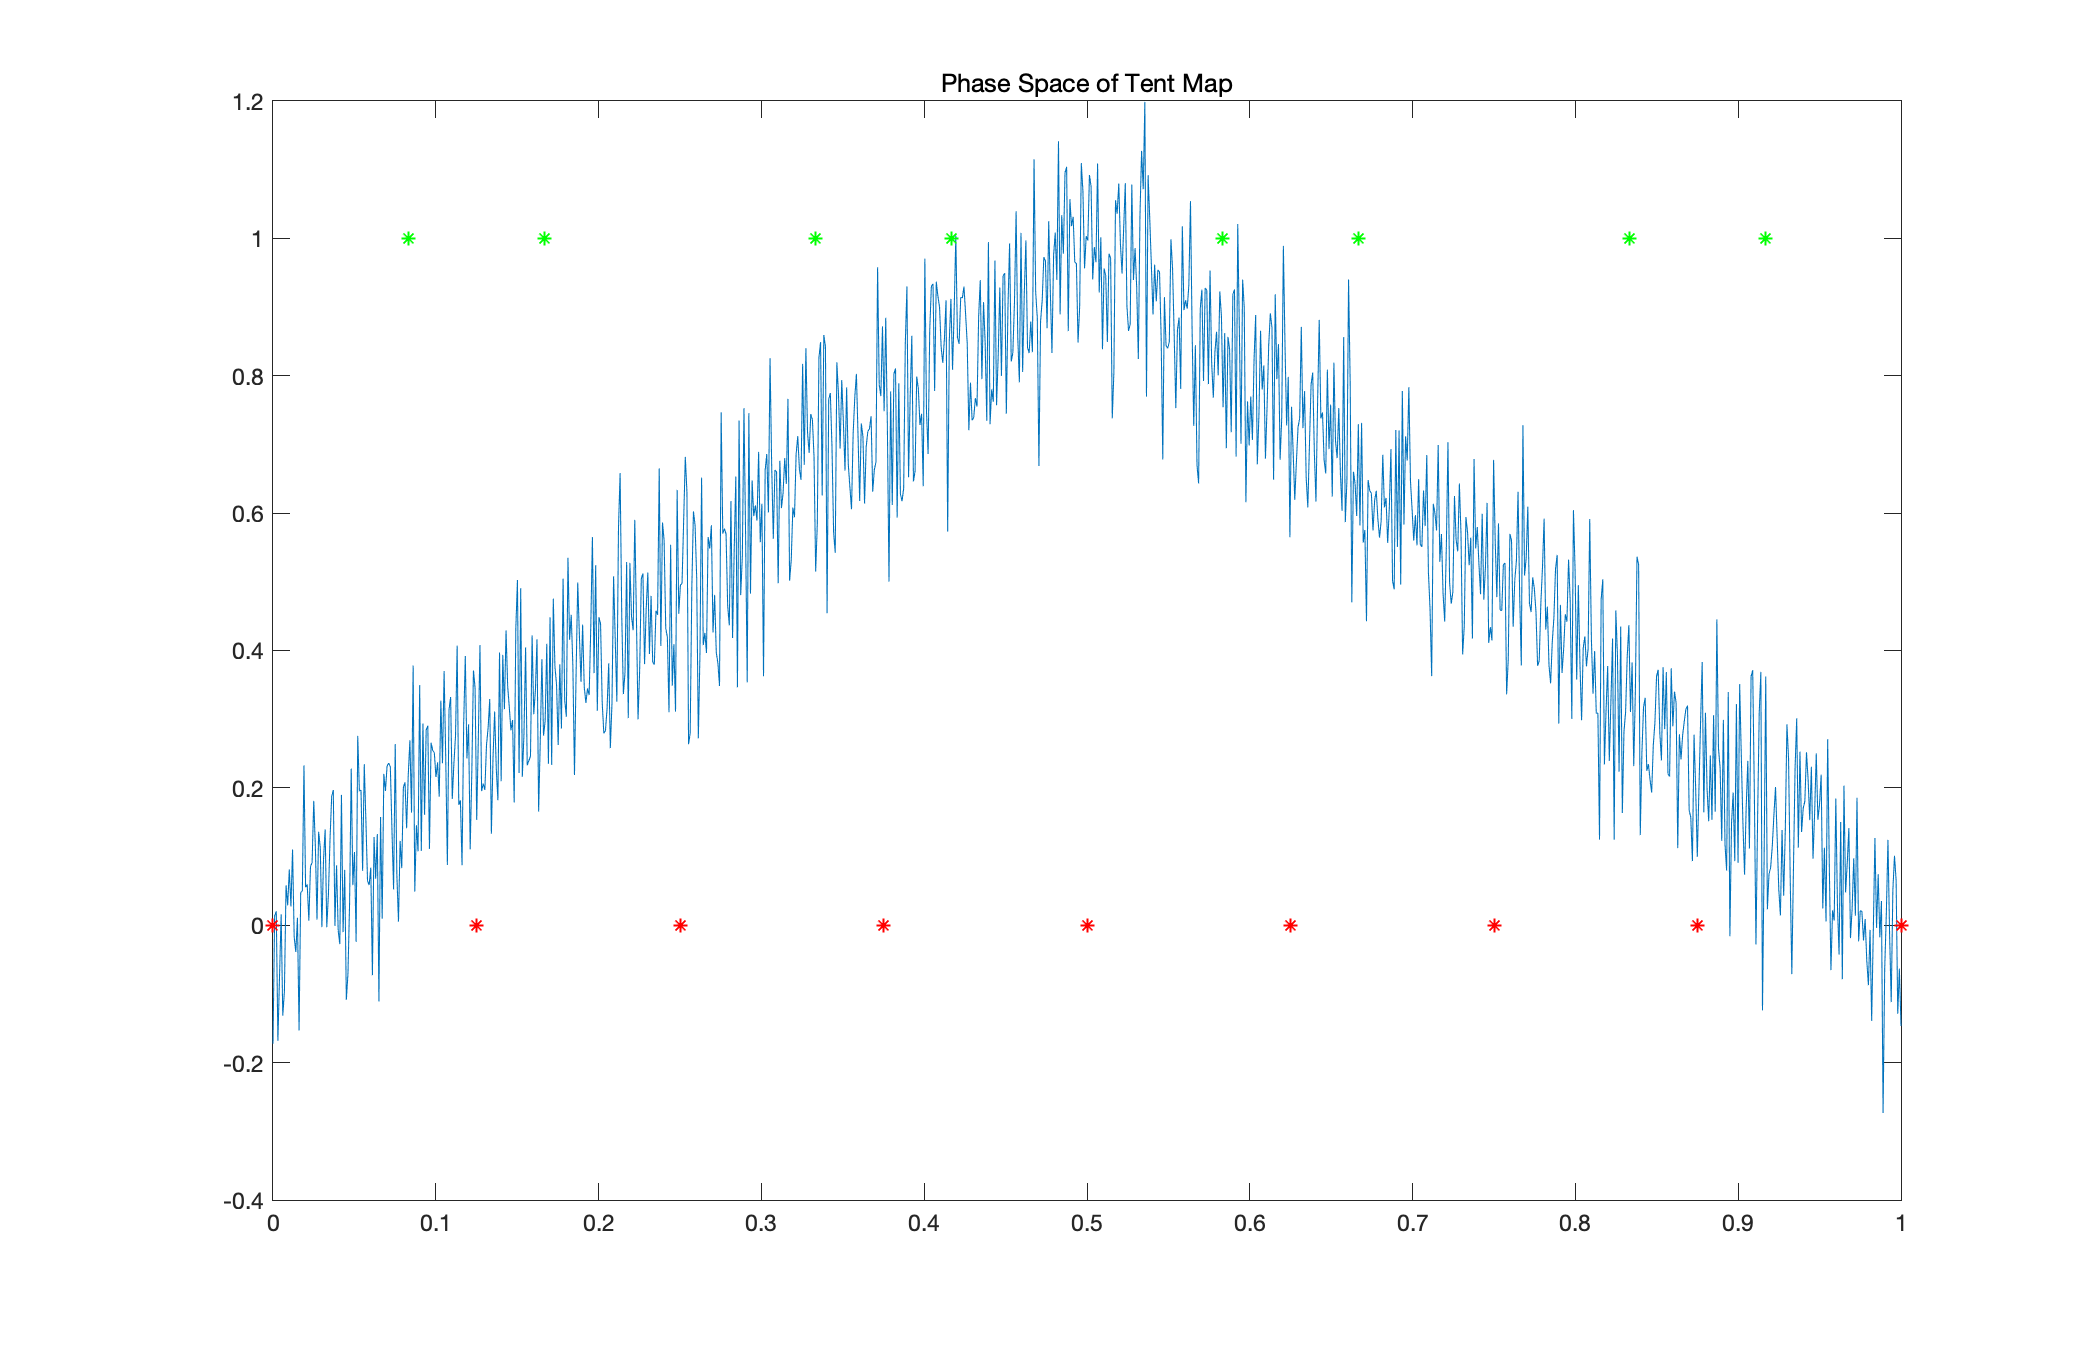
\includegraphics[scale=0.13]{tent/noise/Tent_noise_phase_d0-01}}
  \caption[帐篷映射不同噪声下的相空间]{帐篷映射不同噪声下的相空间:noise表示噪声与函数幅值之比}
  \label{fig:Tent_noise_phase_d0}
\end{figure}

我们取帐篷映射在$noise=0.001$与$noise=0.01$时Koopman算符对应的本征函数,如图\ref{fig:Tent_eigen_noise_n1000m20d0-001}与图\ref{fig:Tent_eigen_noise_n1000m20d0-01}。同样我们在图中标出本征函数极值点的位置,及帐篷映射边界点的位置,对比图\ref{fig:Tent_eigen_noise_n1000m2d0}来探究Koopman算符对边界点划分的鲁棒性。同时,我们在计算Koopman算符的矩阵表示时每次从$K$到$L$进行了多次的演化,并取演化的平均值,即由于涨落的影响,我们每次的演化变为了一个高斯波包的分布,这样可以减少噪声对本征函数图像图像的随机性。

\begin{figure}[!]
  \centering%[2,3,4,5,8,10,15,20]
  \subfloat[m=2]{
    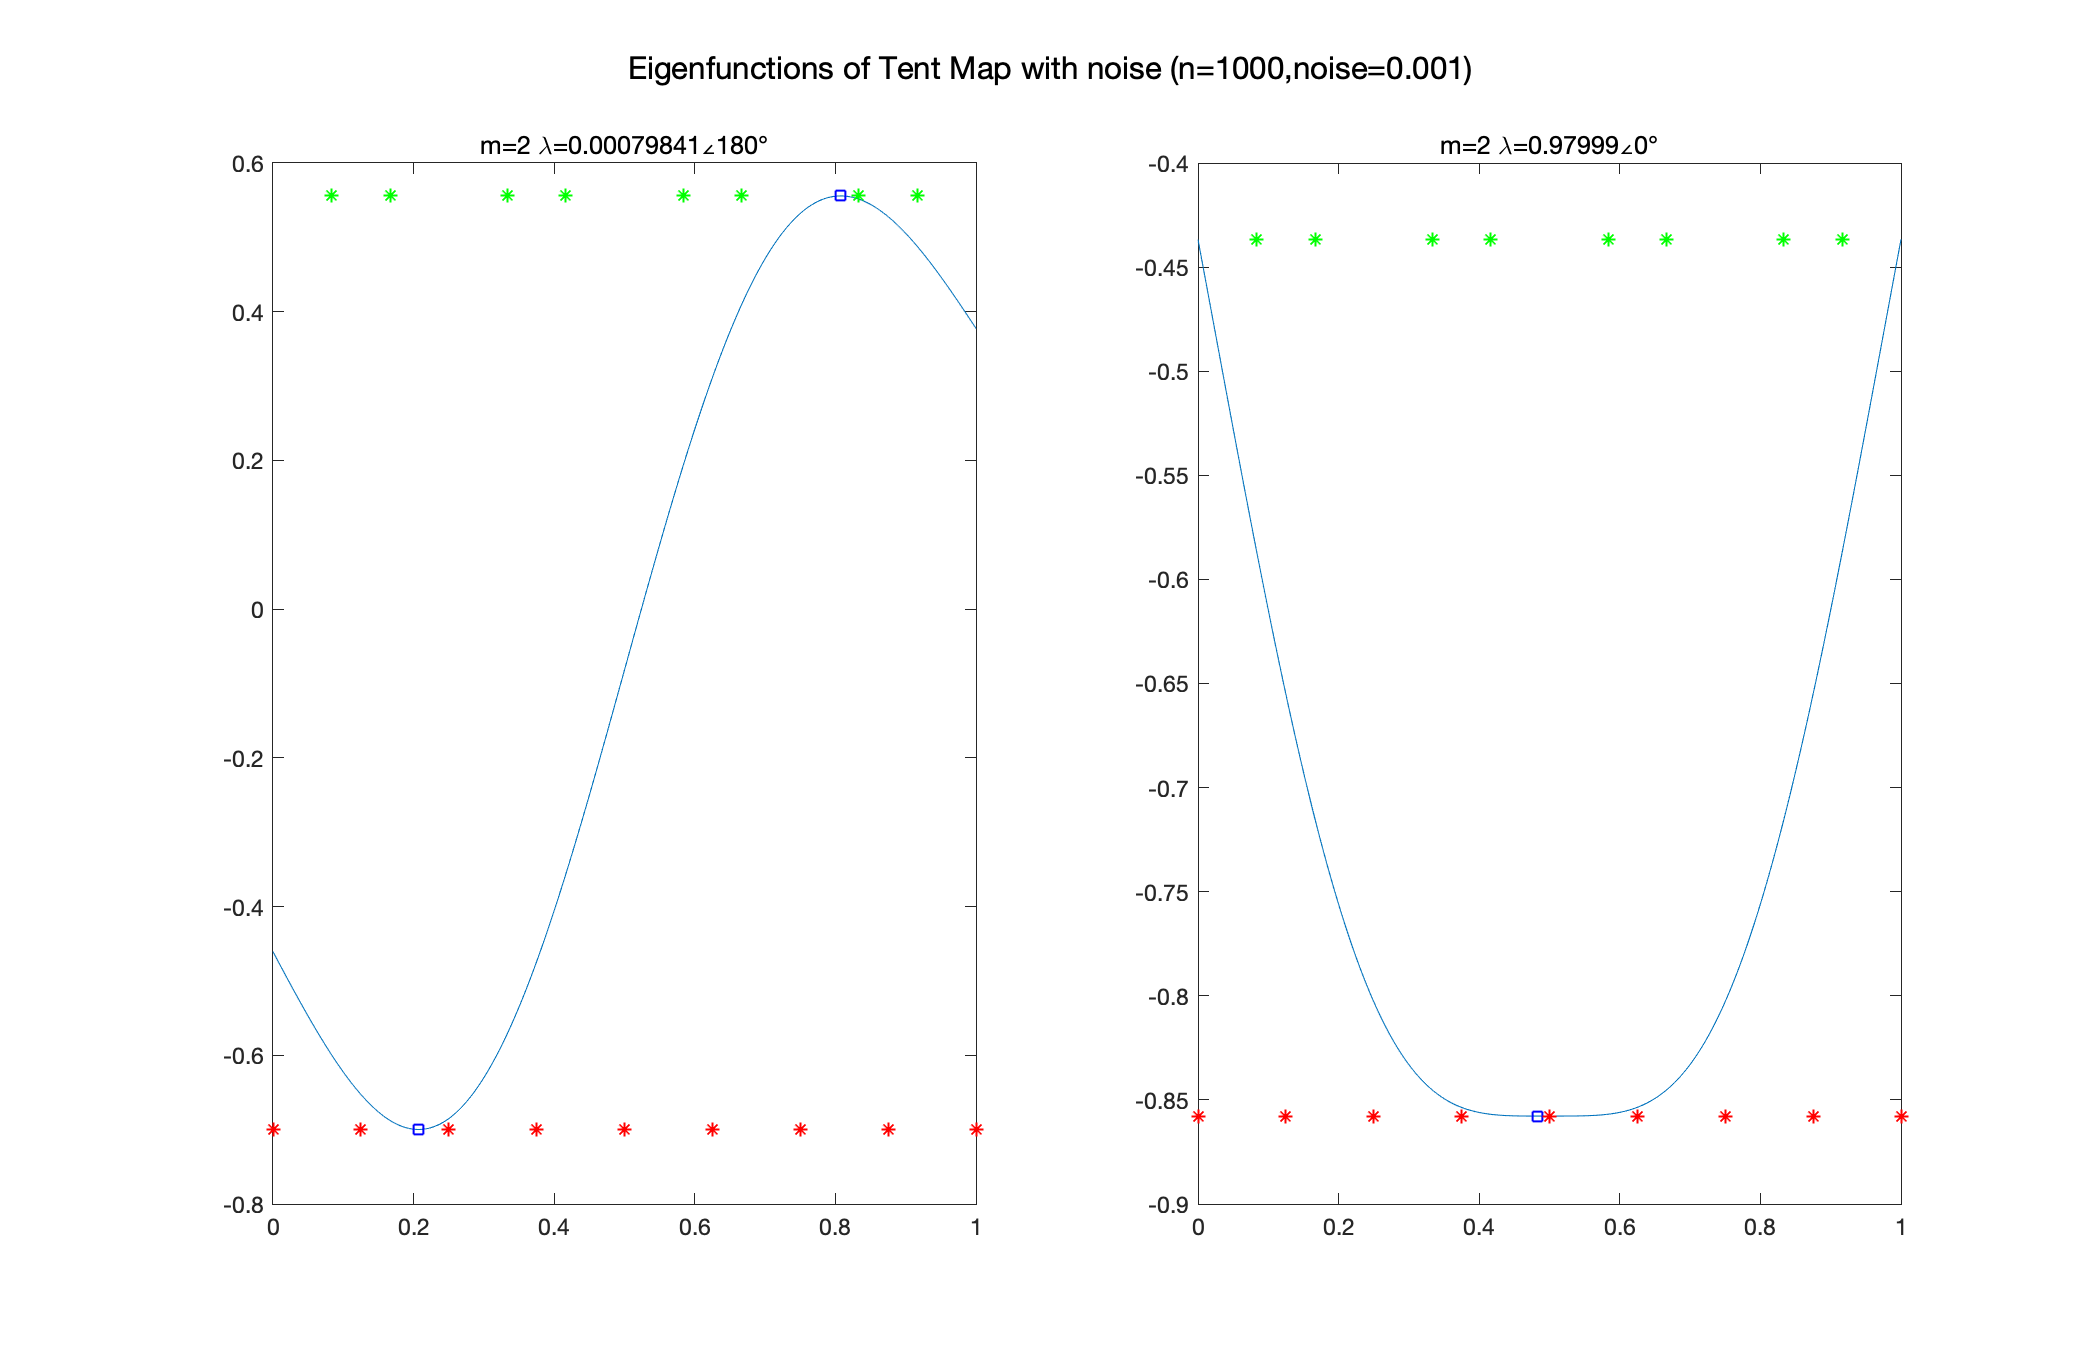
\includegraphics[scale=0.2]{tent/noise/Tent_eigen_noise_n1000m2d0-001}}
  \subfloat[m=3]{
    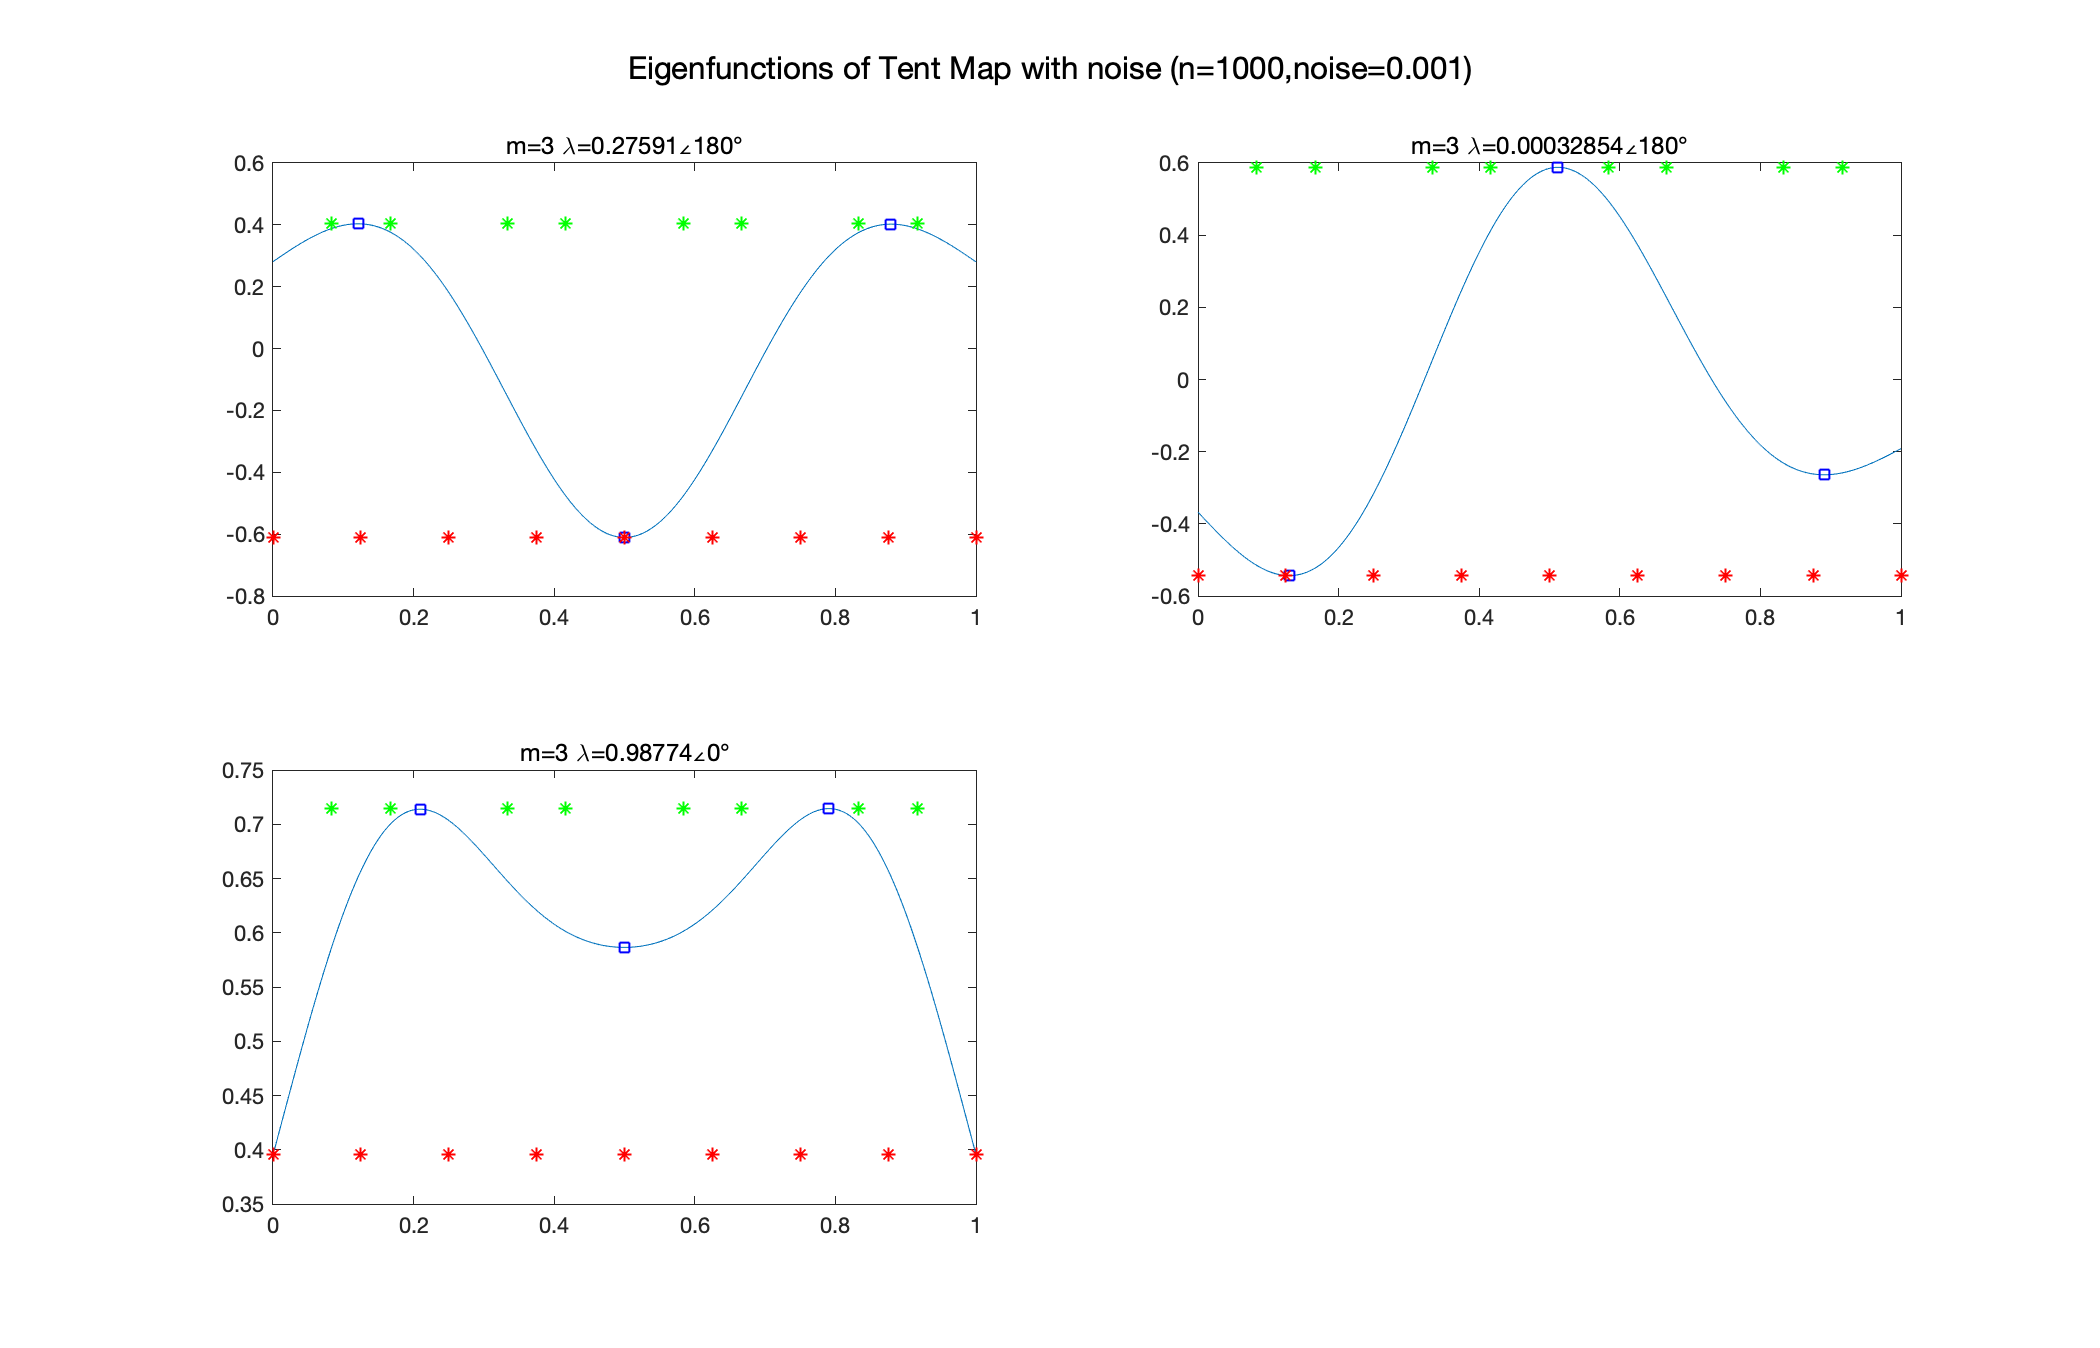
\includegraphics[scale=0.2]{tent/noise/Tent_eigen_noise_n1000m3d0-001}}
    \\
  \subfloat[m=4]{
    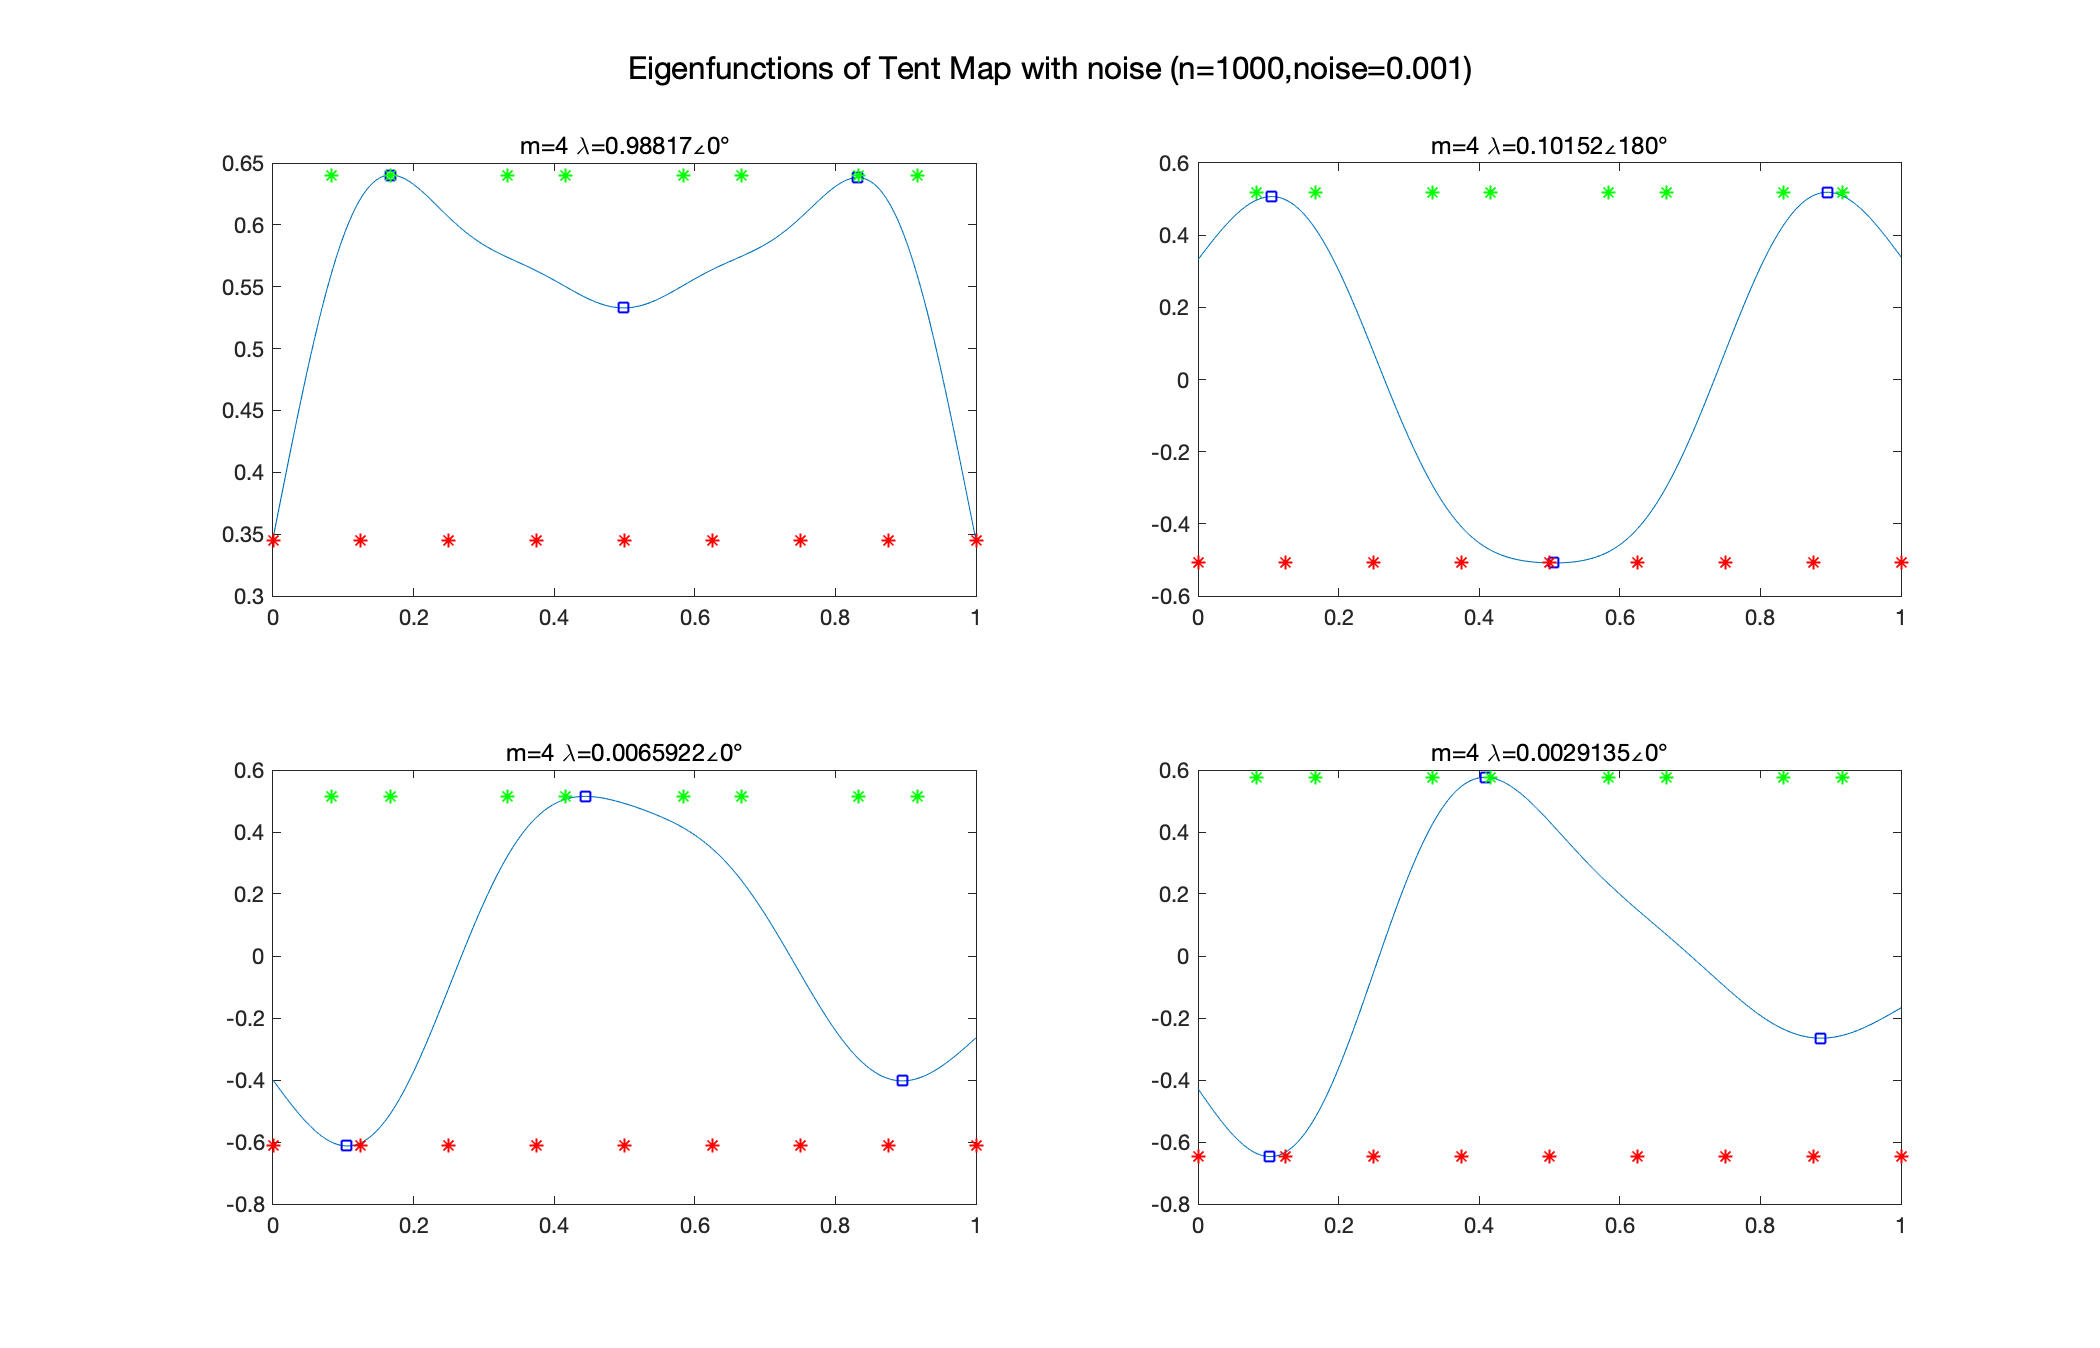
\includegraphics[scale=0.2]{tent/noise/Tent_eigen_noise_n1000m4d0-001}}
  \subfloat[m=5]{
    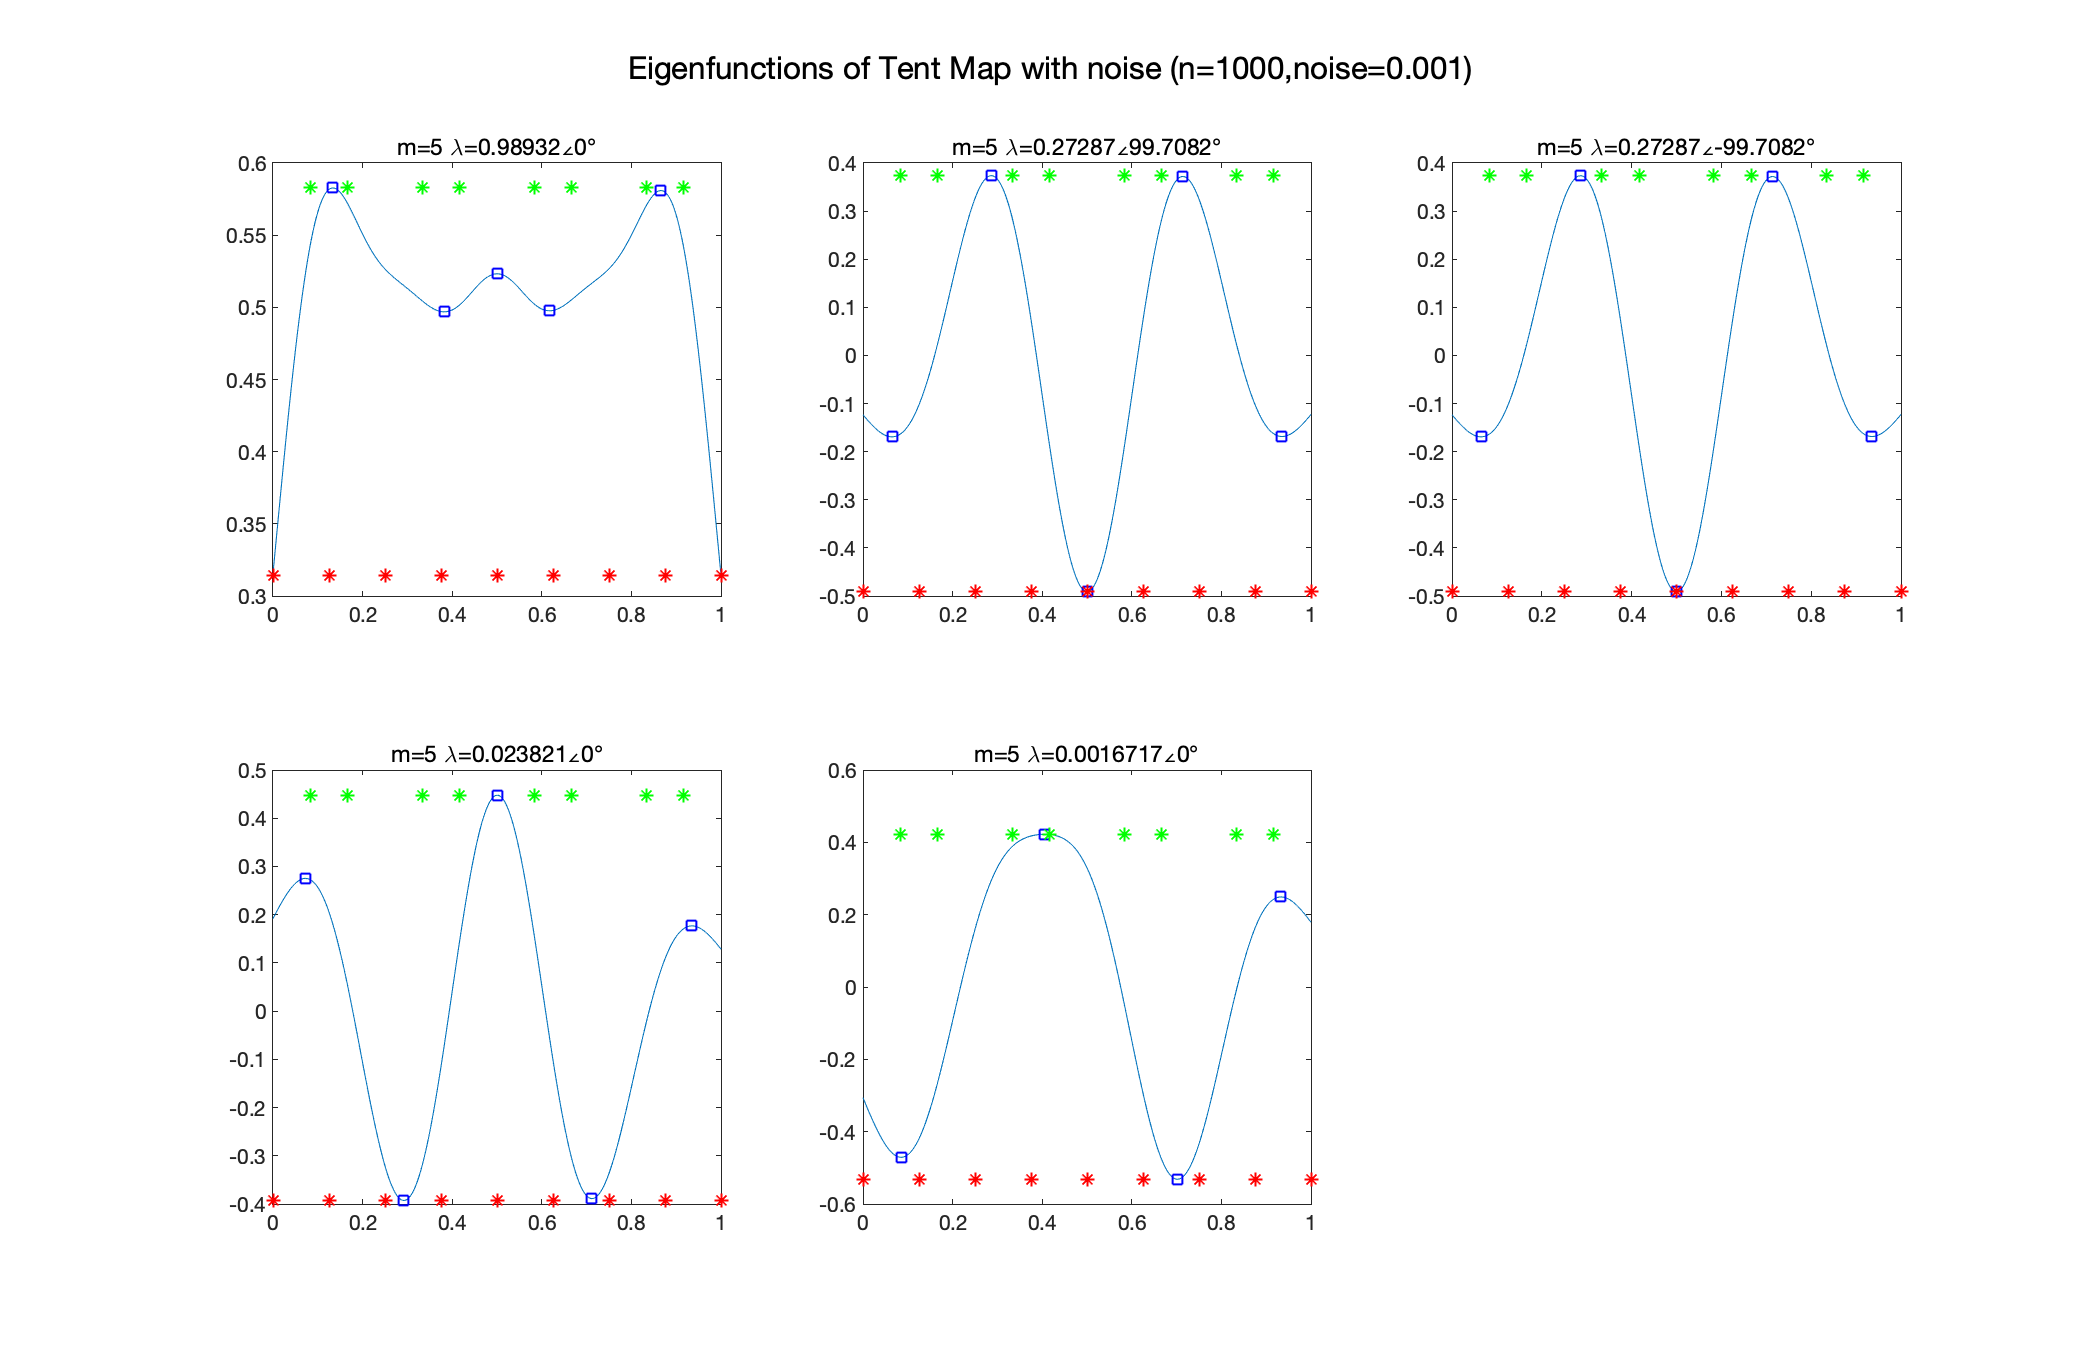
\includegraphics[scale=0.2]{tent/noise/Tent_eigen_noise_n1000m5d0-001}}
    \\
  \subfloat[m=8]{
    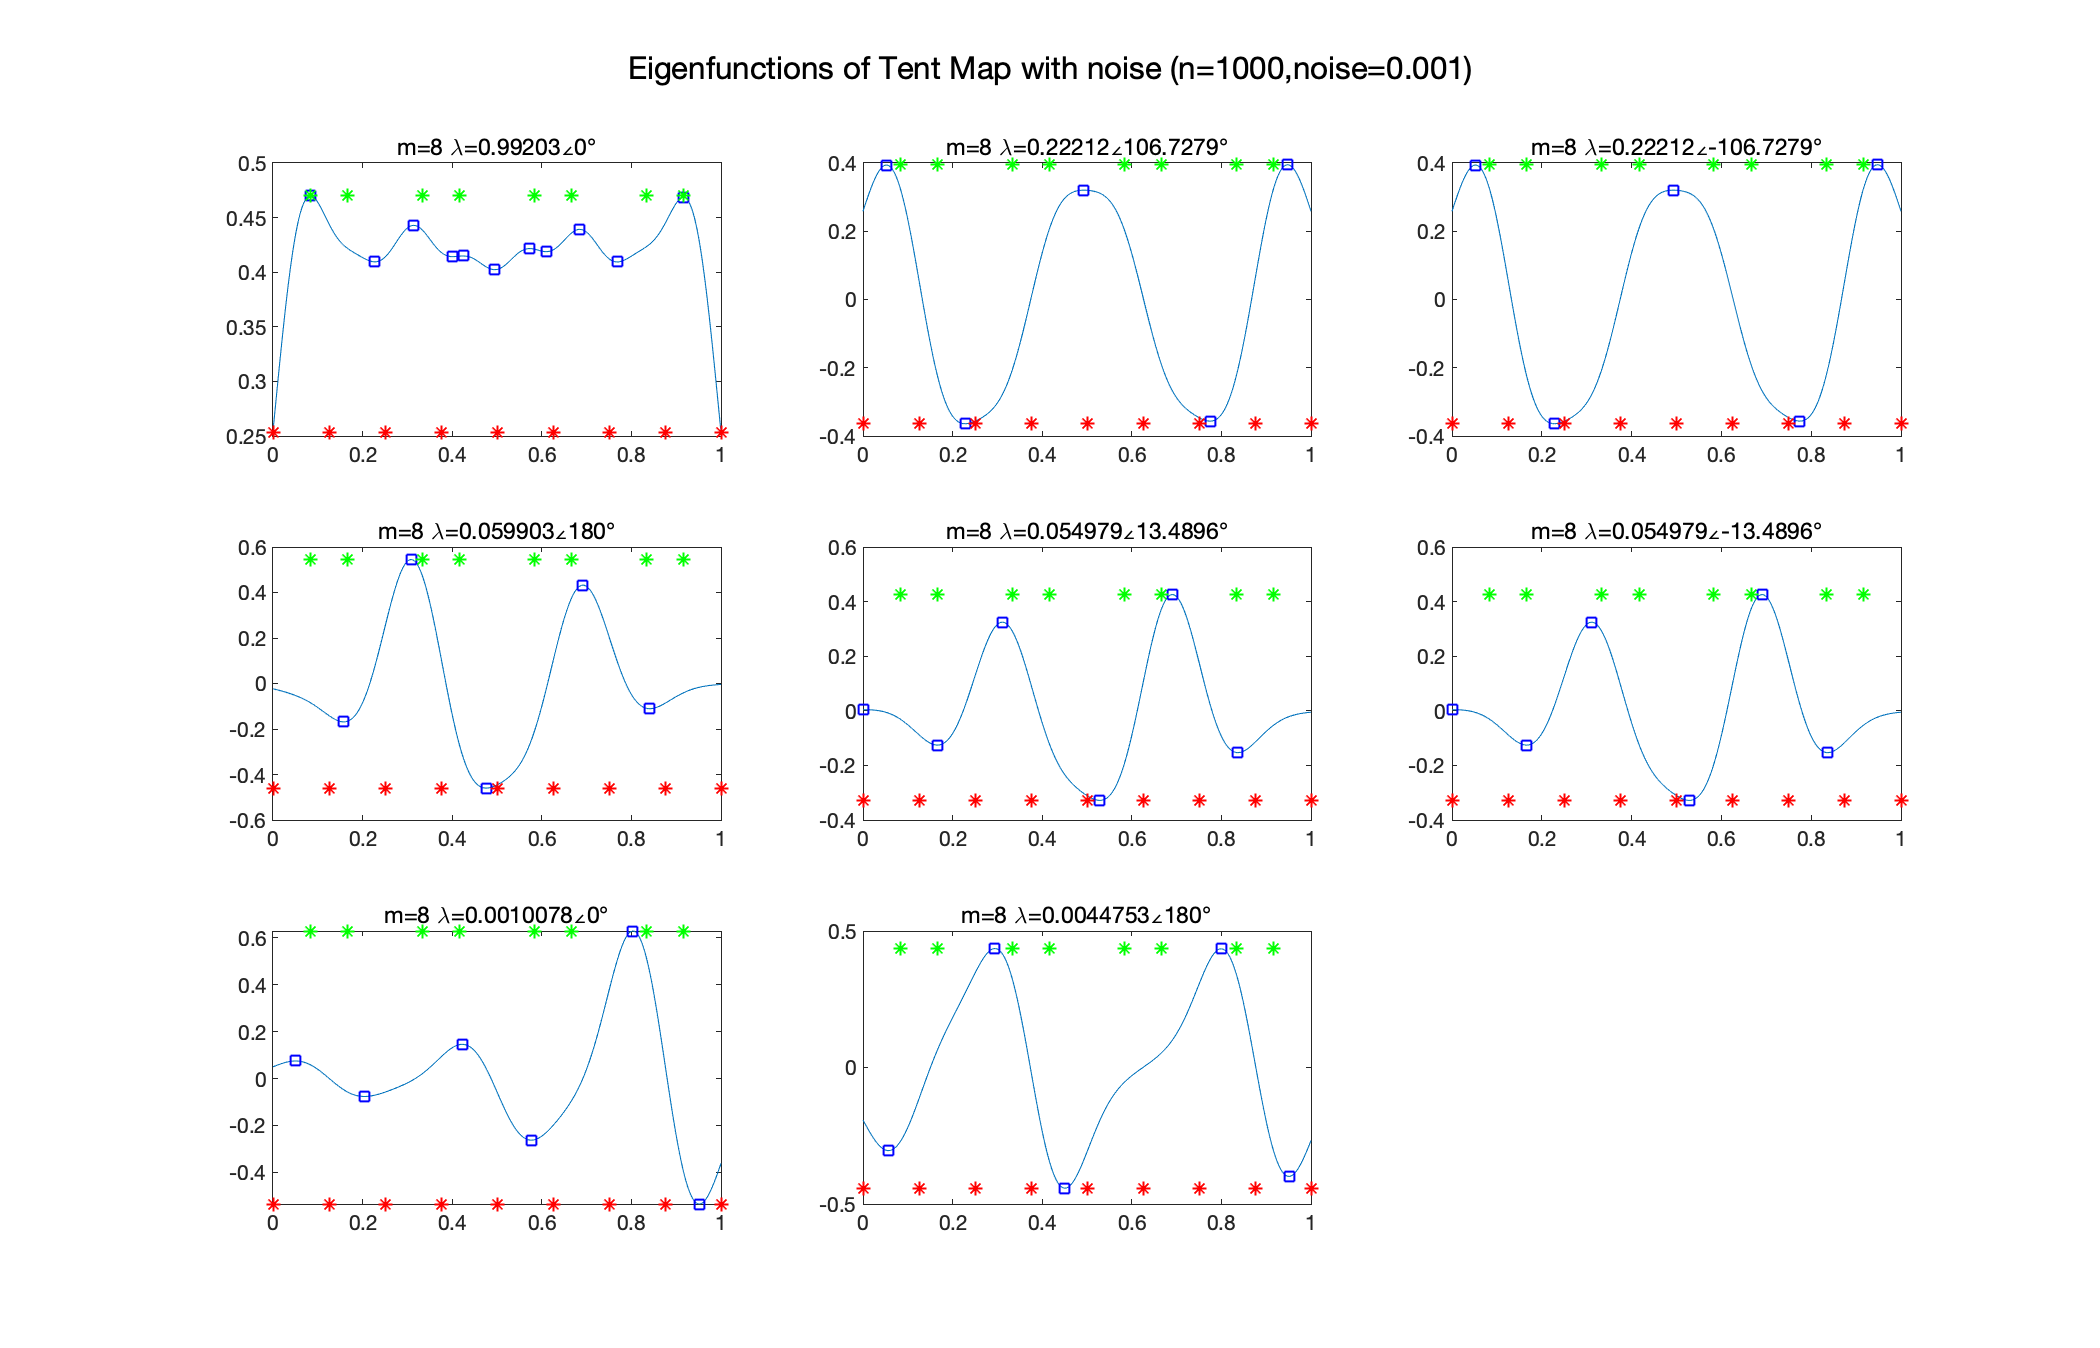
\includegraphics[scale=0.2]{tent/noise/Tent_eigen_noise_n1000m8d0-001}}
  \subfloat[m=10]{
    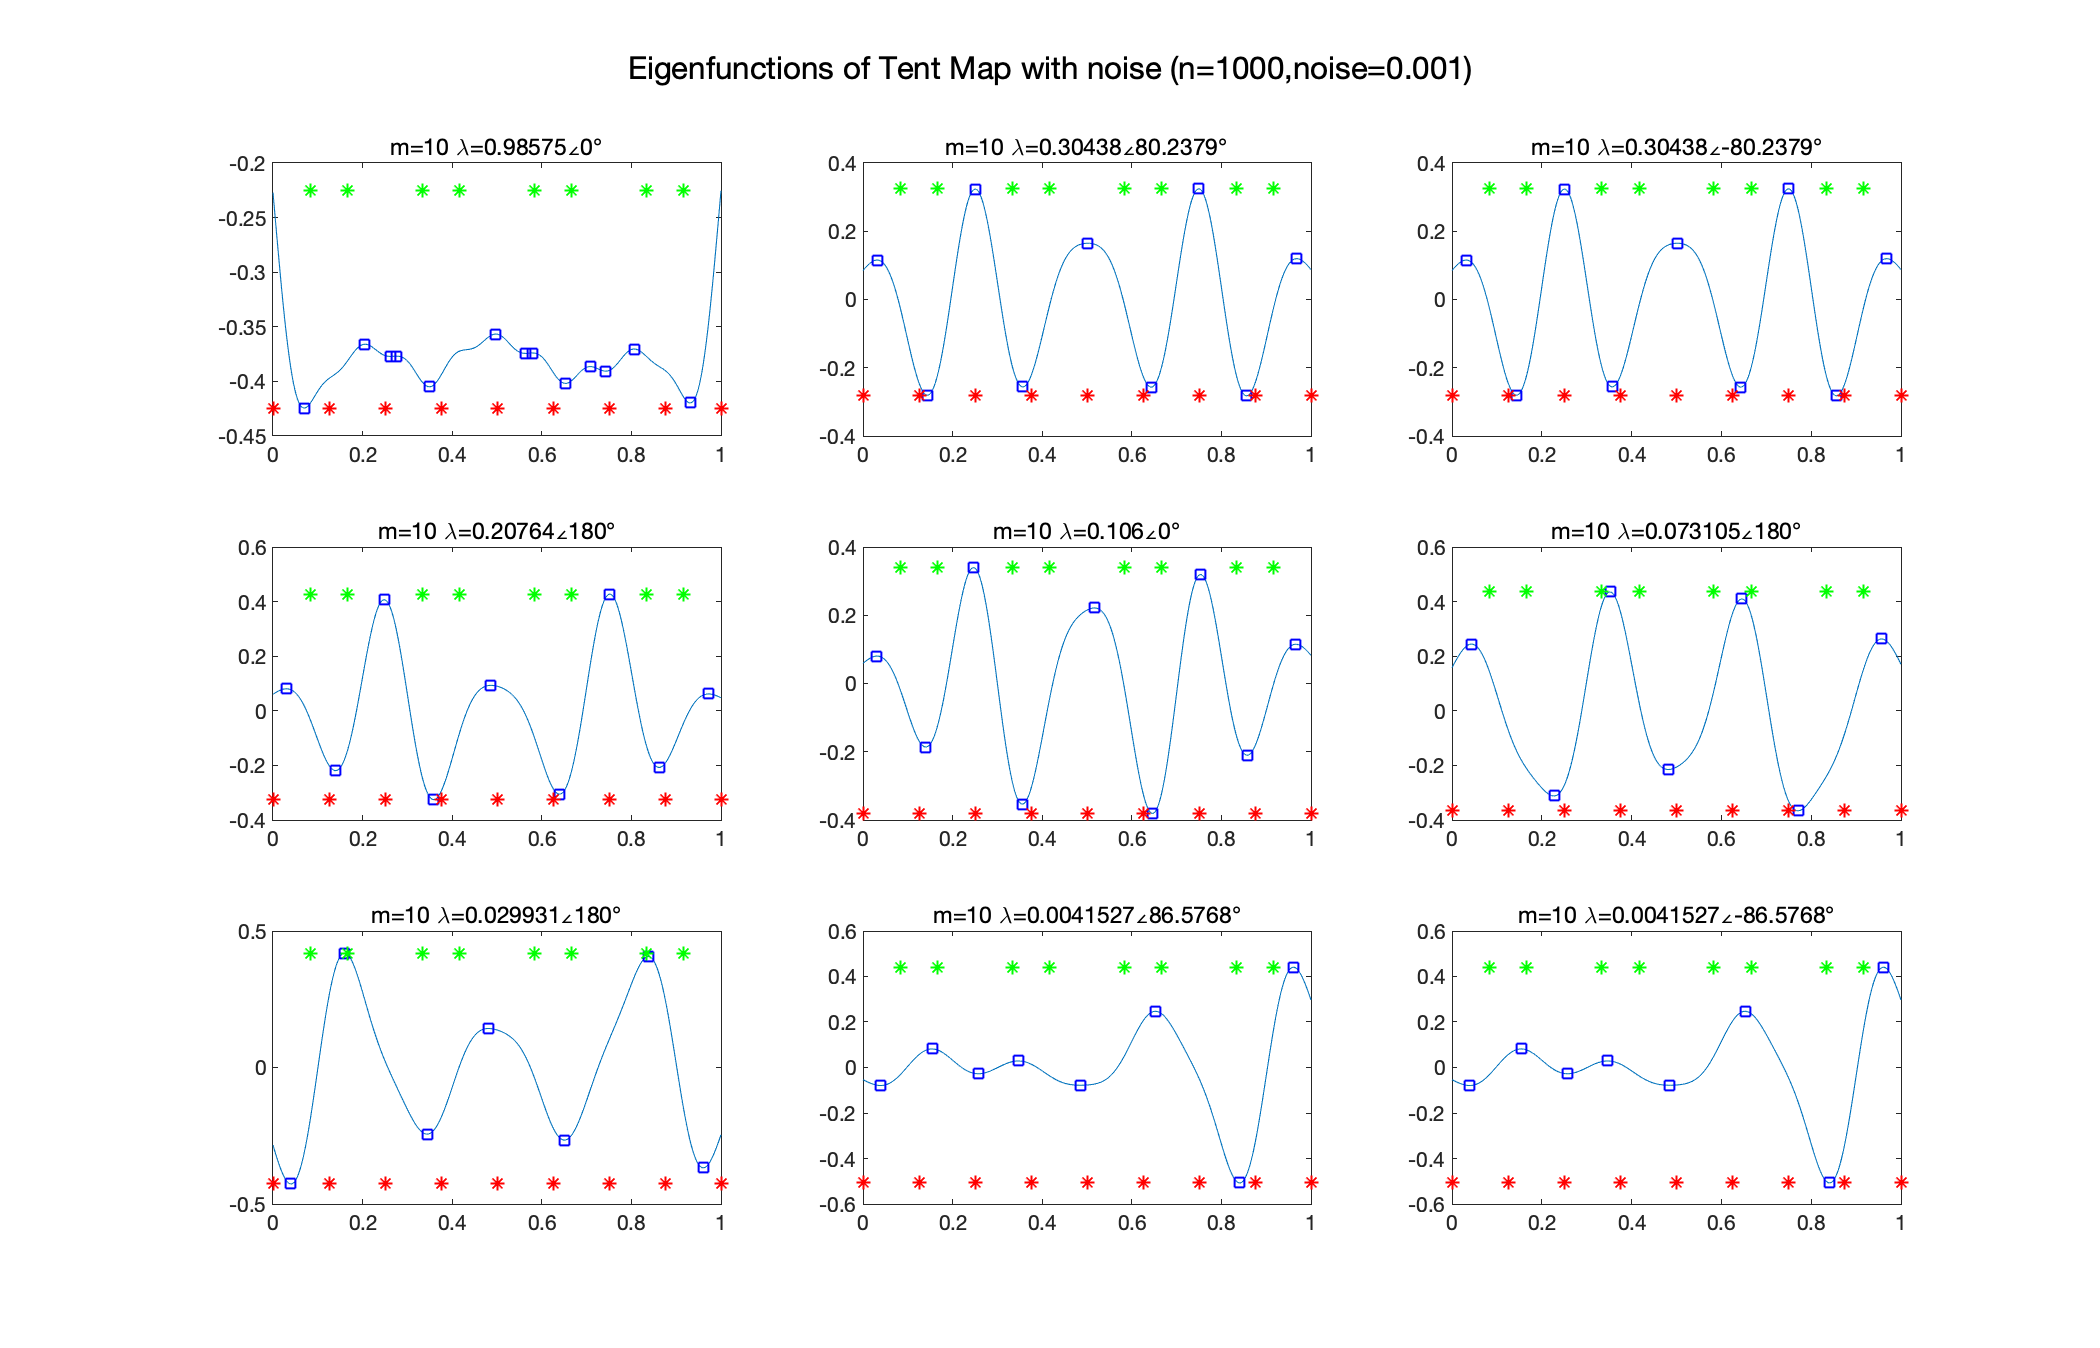
\includegraphics[scale=0.2]{tent/noise/Tent_eigen_noise_n1000m10d0-001}}
    \\
  \subfloat[m=15]{
    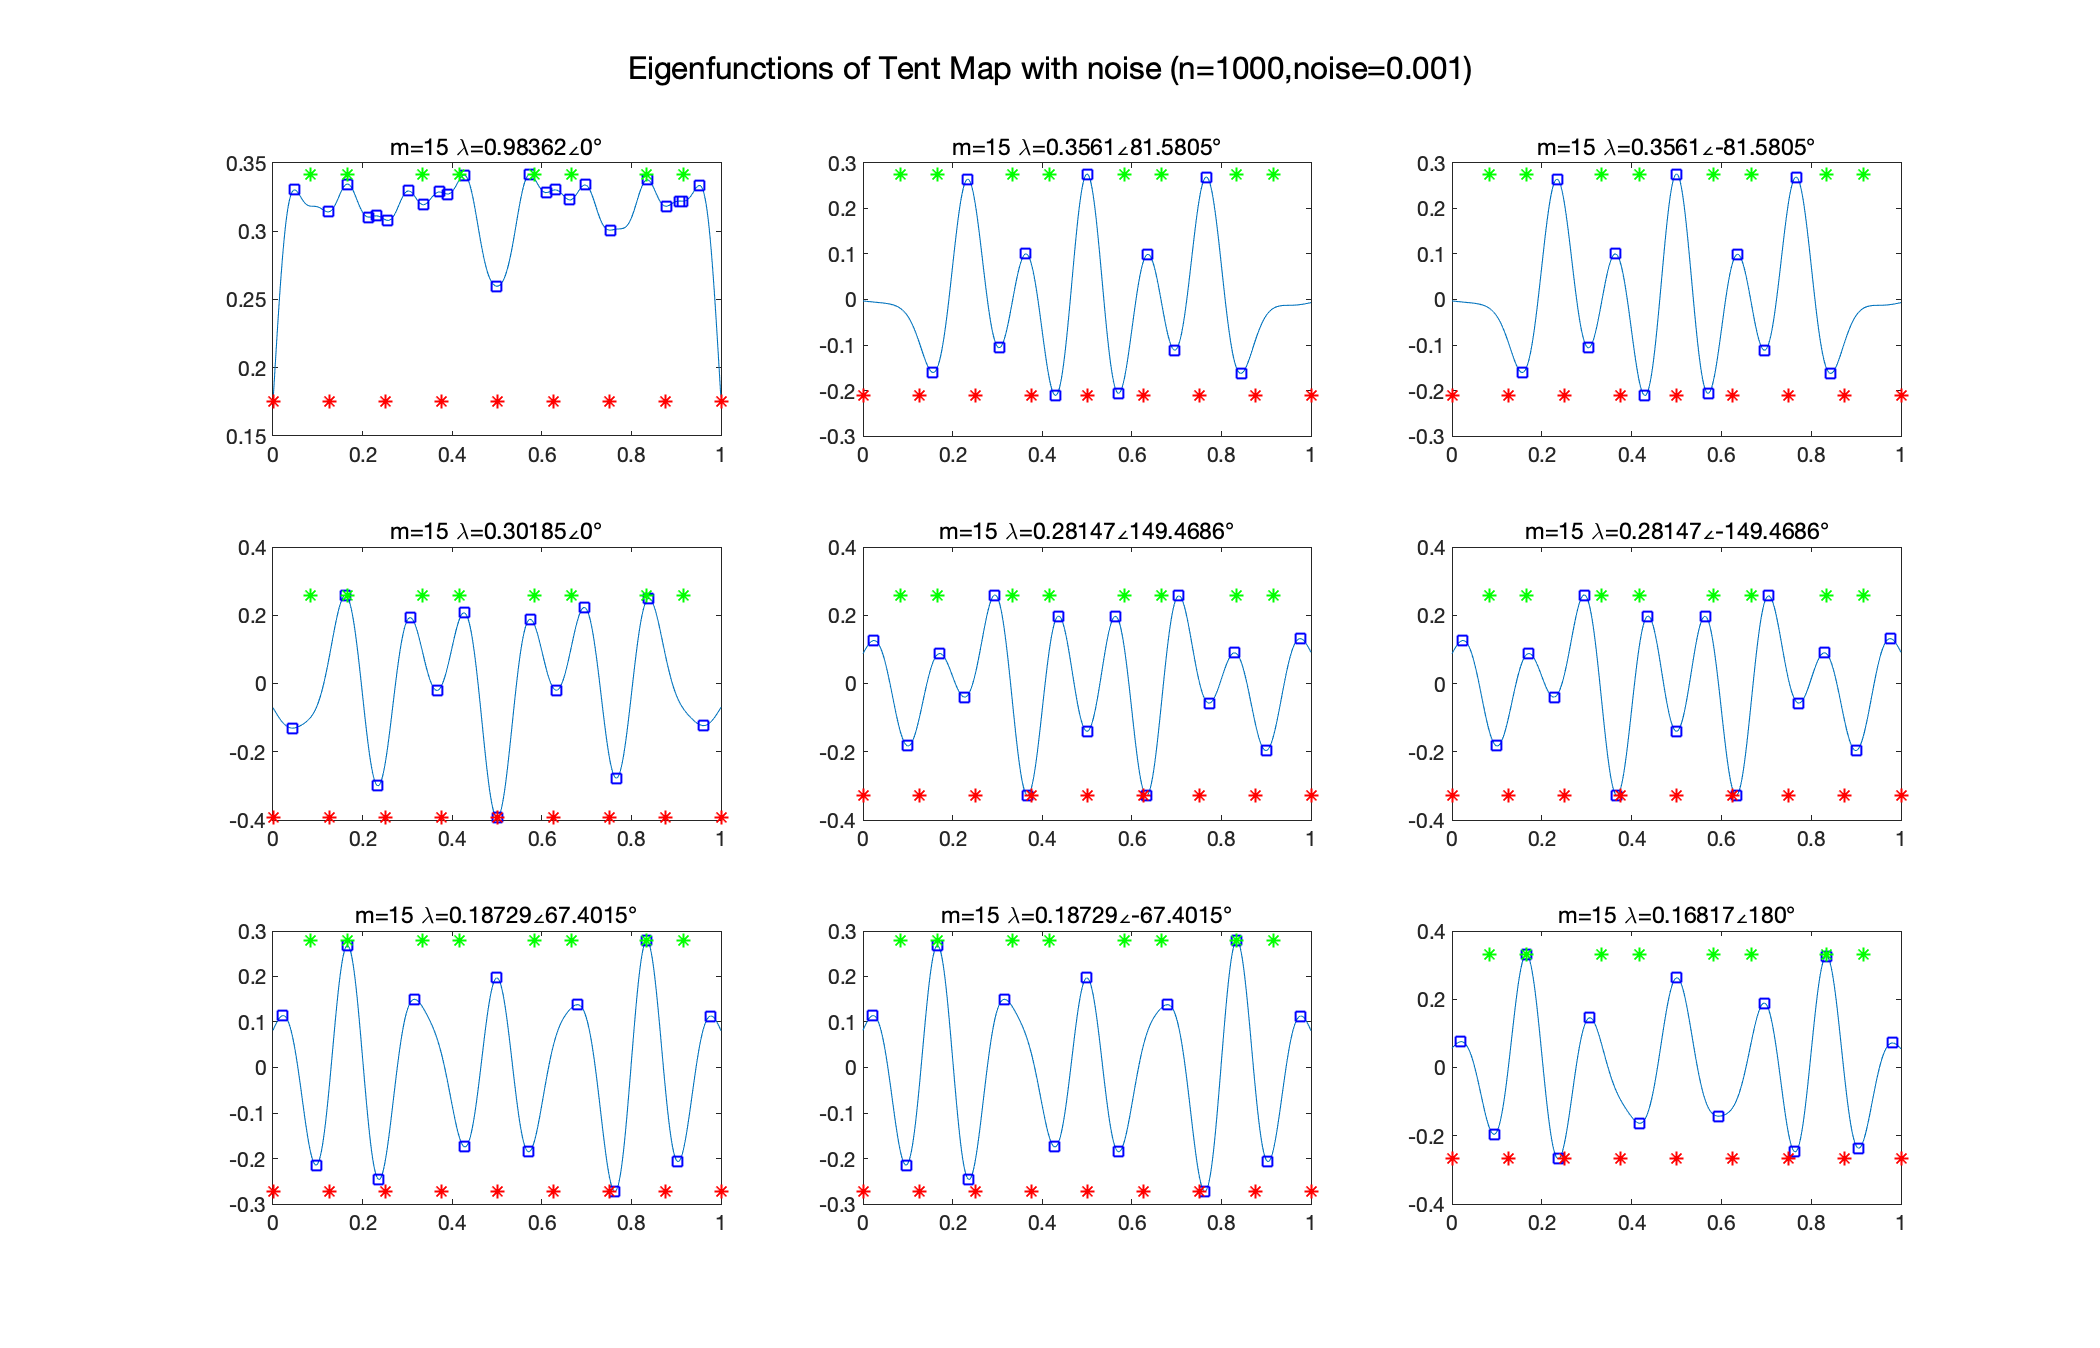
\includegraphics[scale=0.2]{tent/noise/Tent_eigen_noise_n1000m15d0-001}}
  \subfloat[m=20]{
    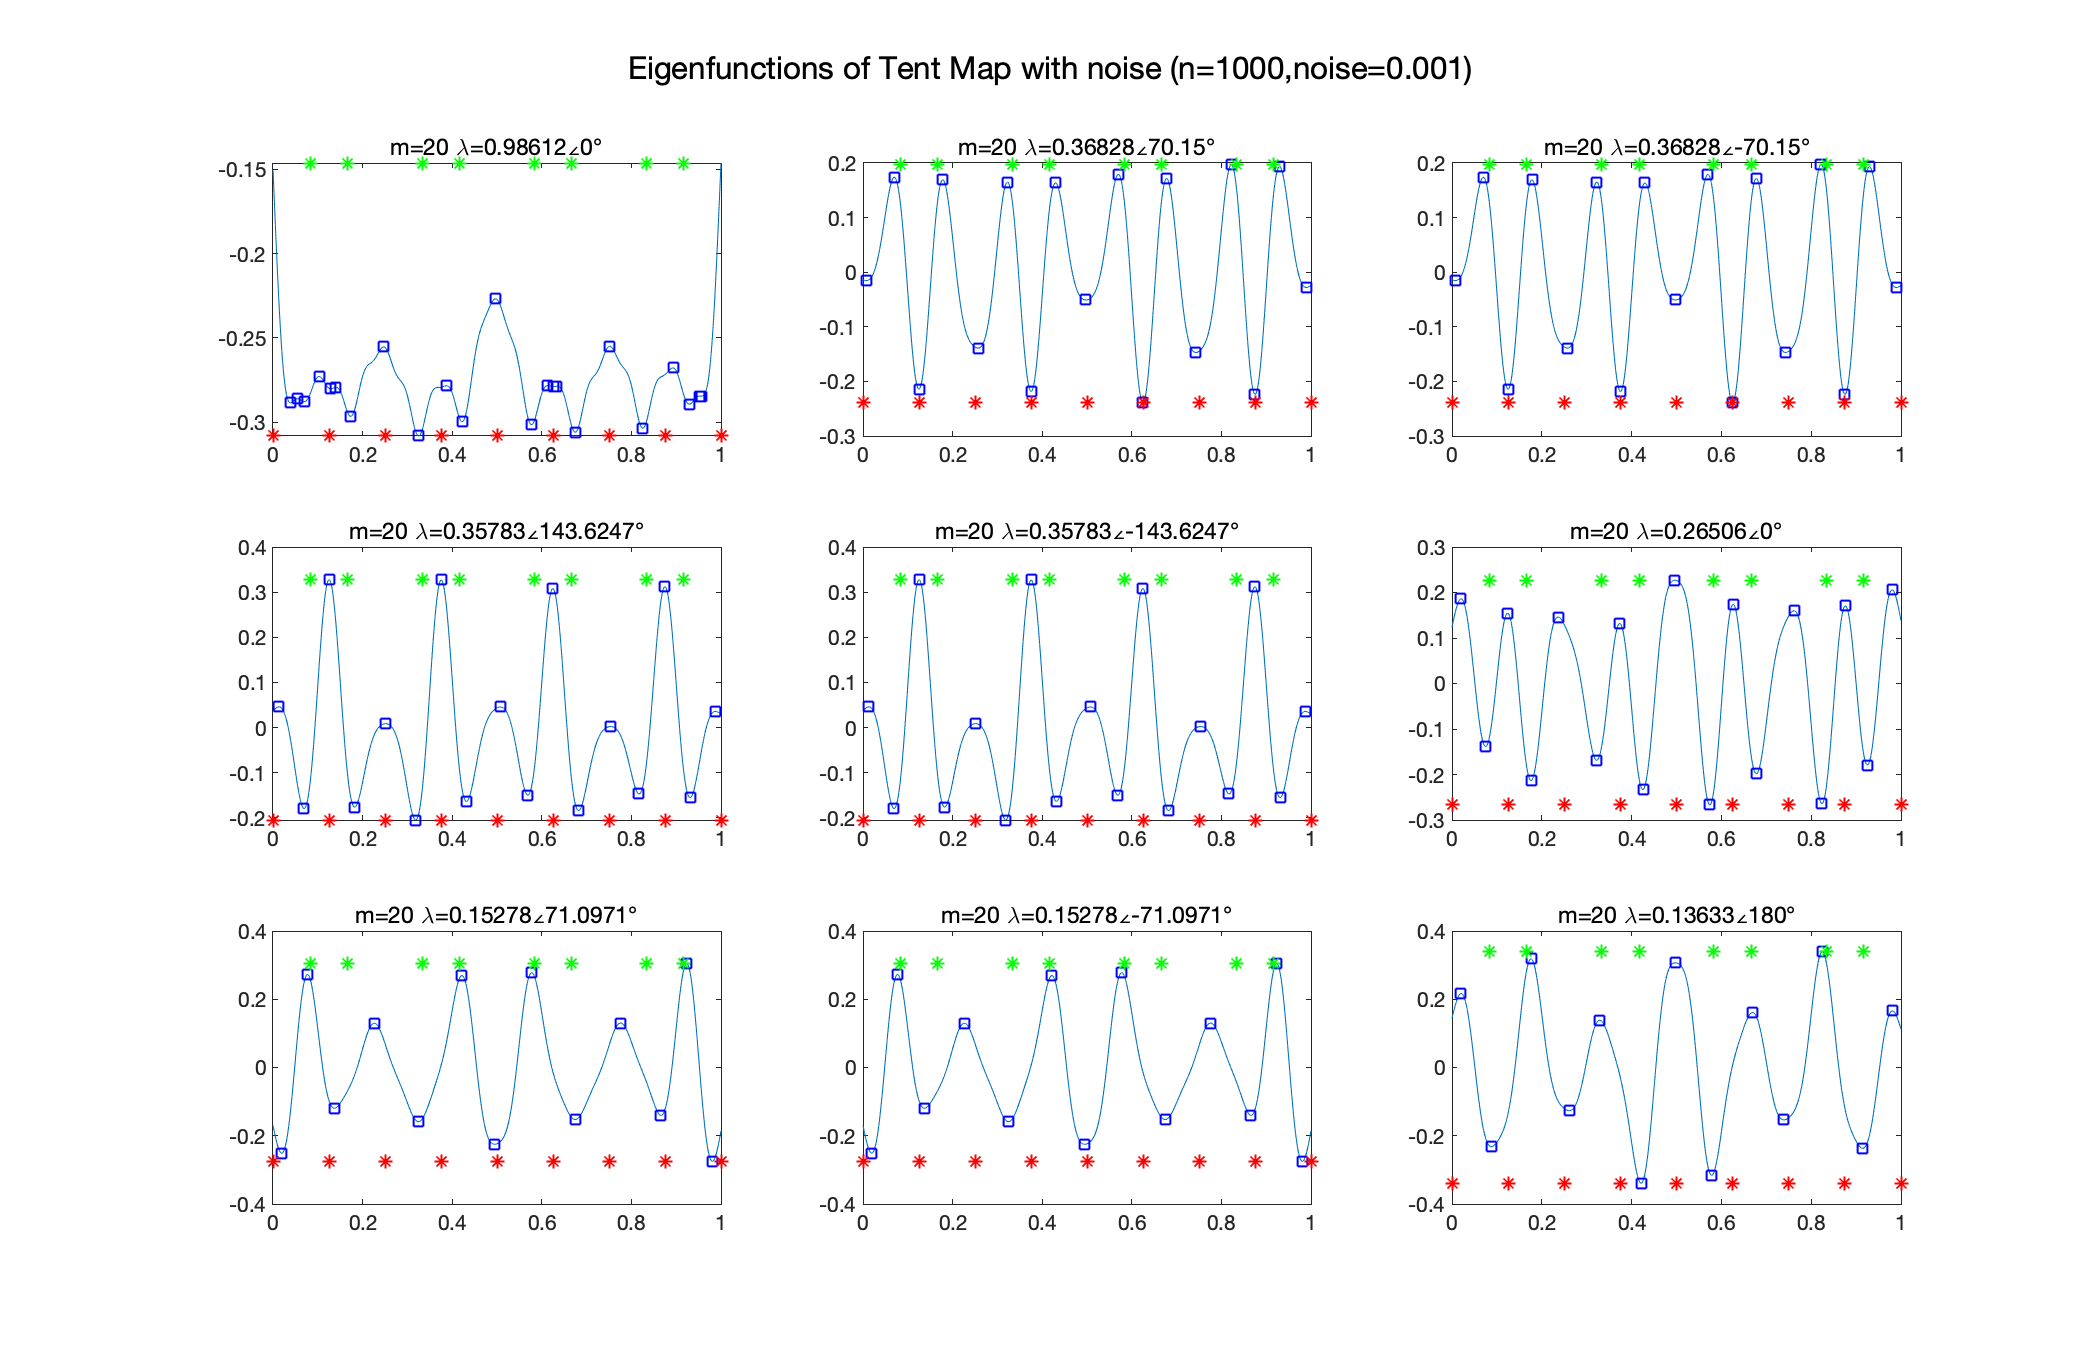
\includegraphics[scale=0.2]{tent/noise/Tent_eigen_noise_n1000m20d0-001}}
    \\
  \caption{帐篷映射的边界点与本征函数($noise=0.001$)}\label{fig:Tent_eigen_noise_n1000m20d0-001}
\end{figure}

\begin{figure}[!]
  \centering%[2,3,4,5,8,10,15,20]
  \subfloat[m=2]{
    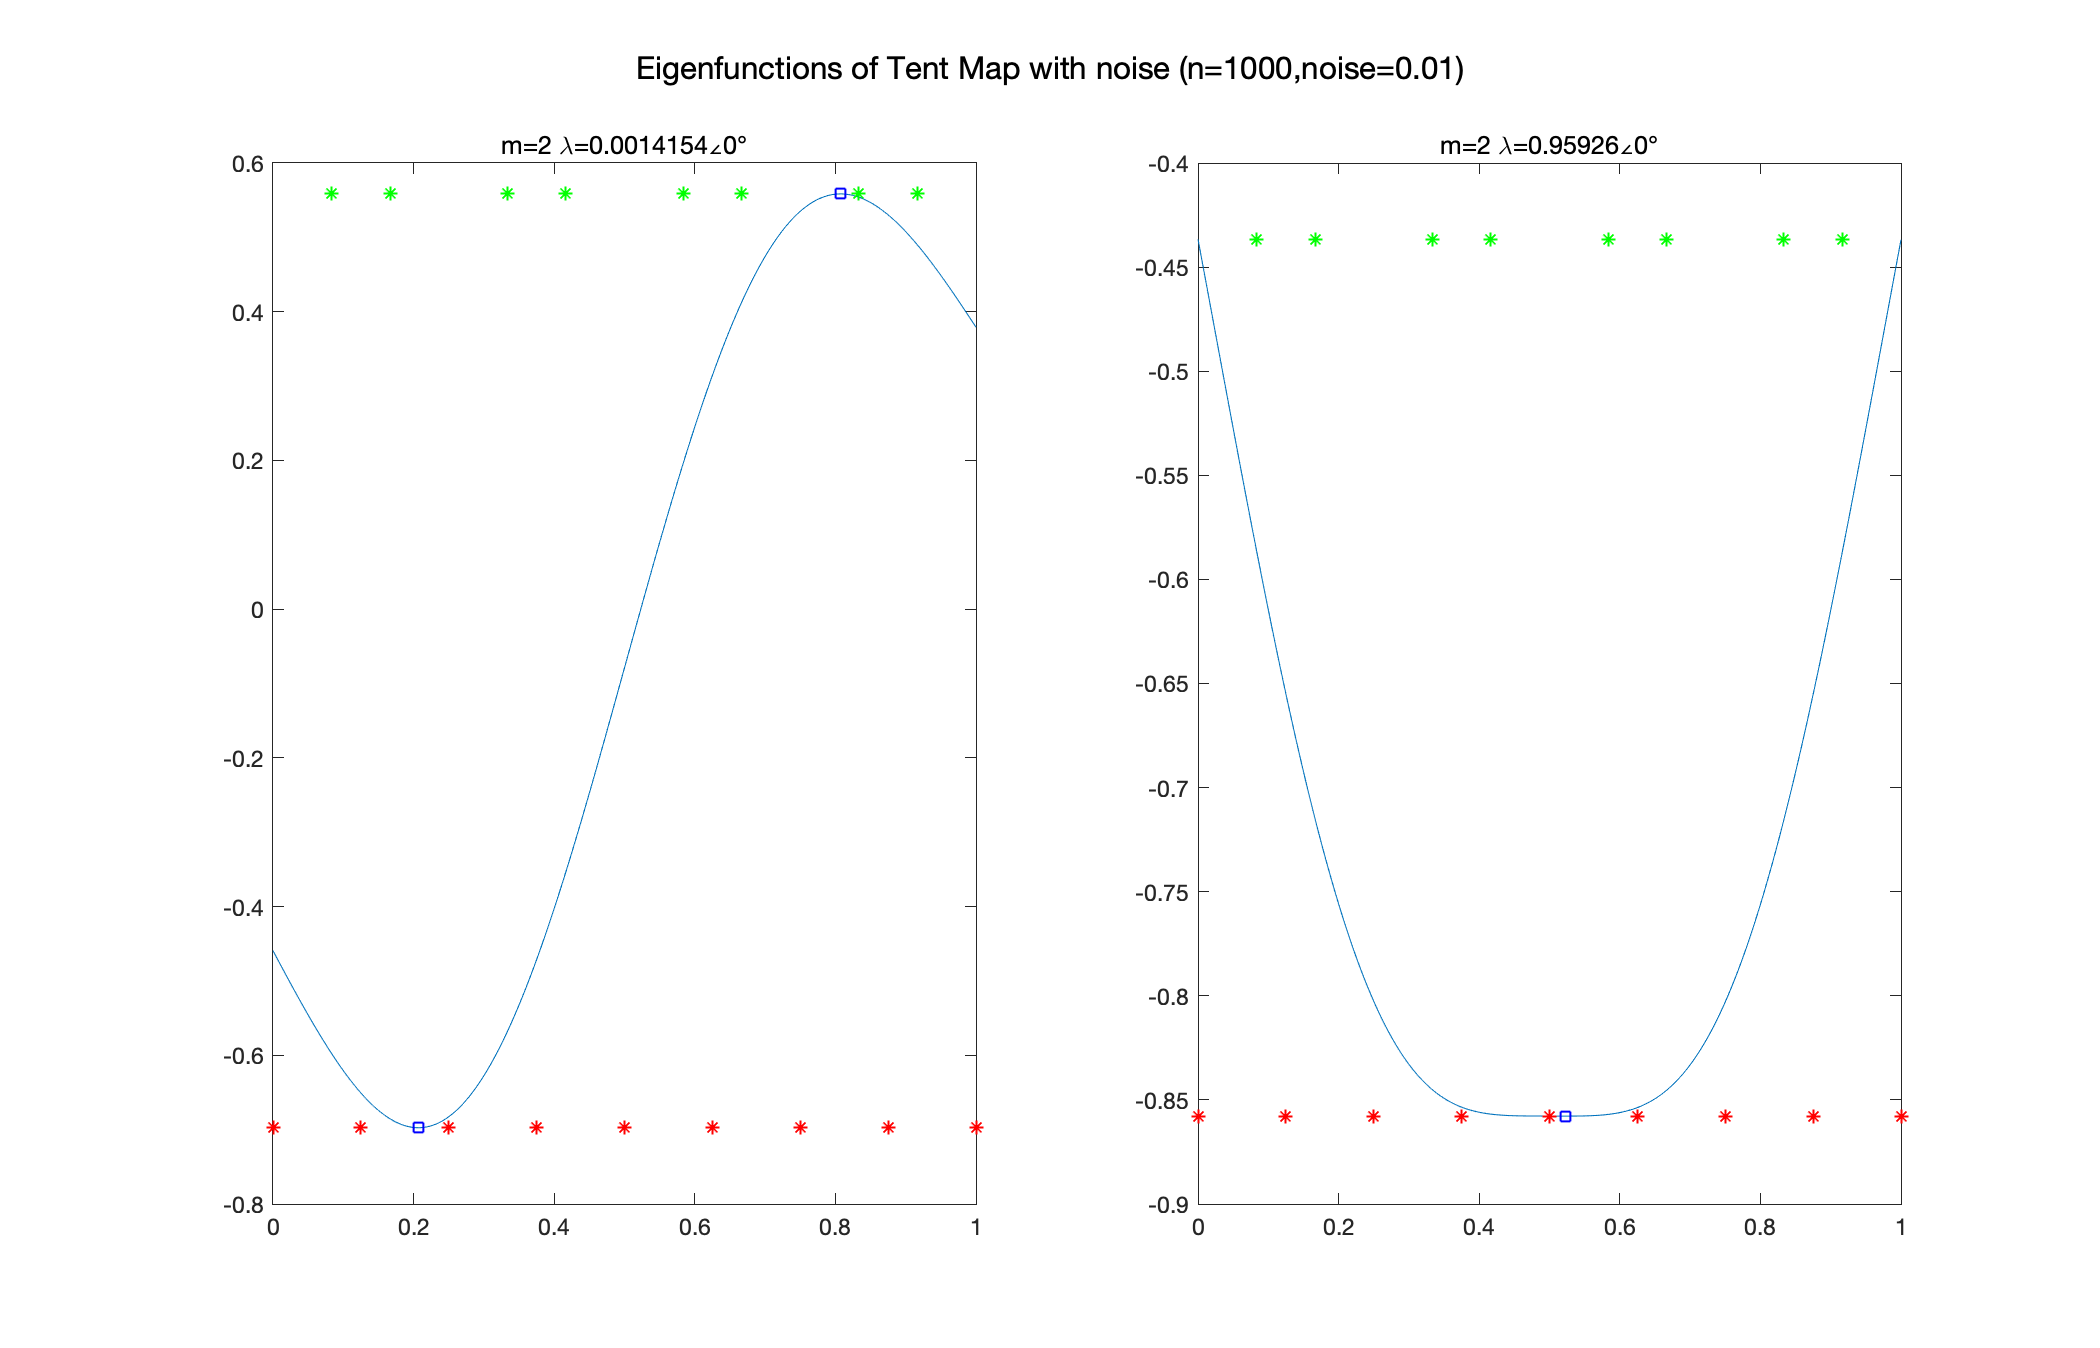
\includegraphics[scale=0.2]{tent/noise/Tent_eigen_noise_n1000m2d0-01}}
  \subfloat[m=3]{
    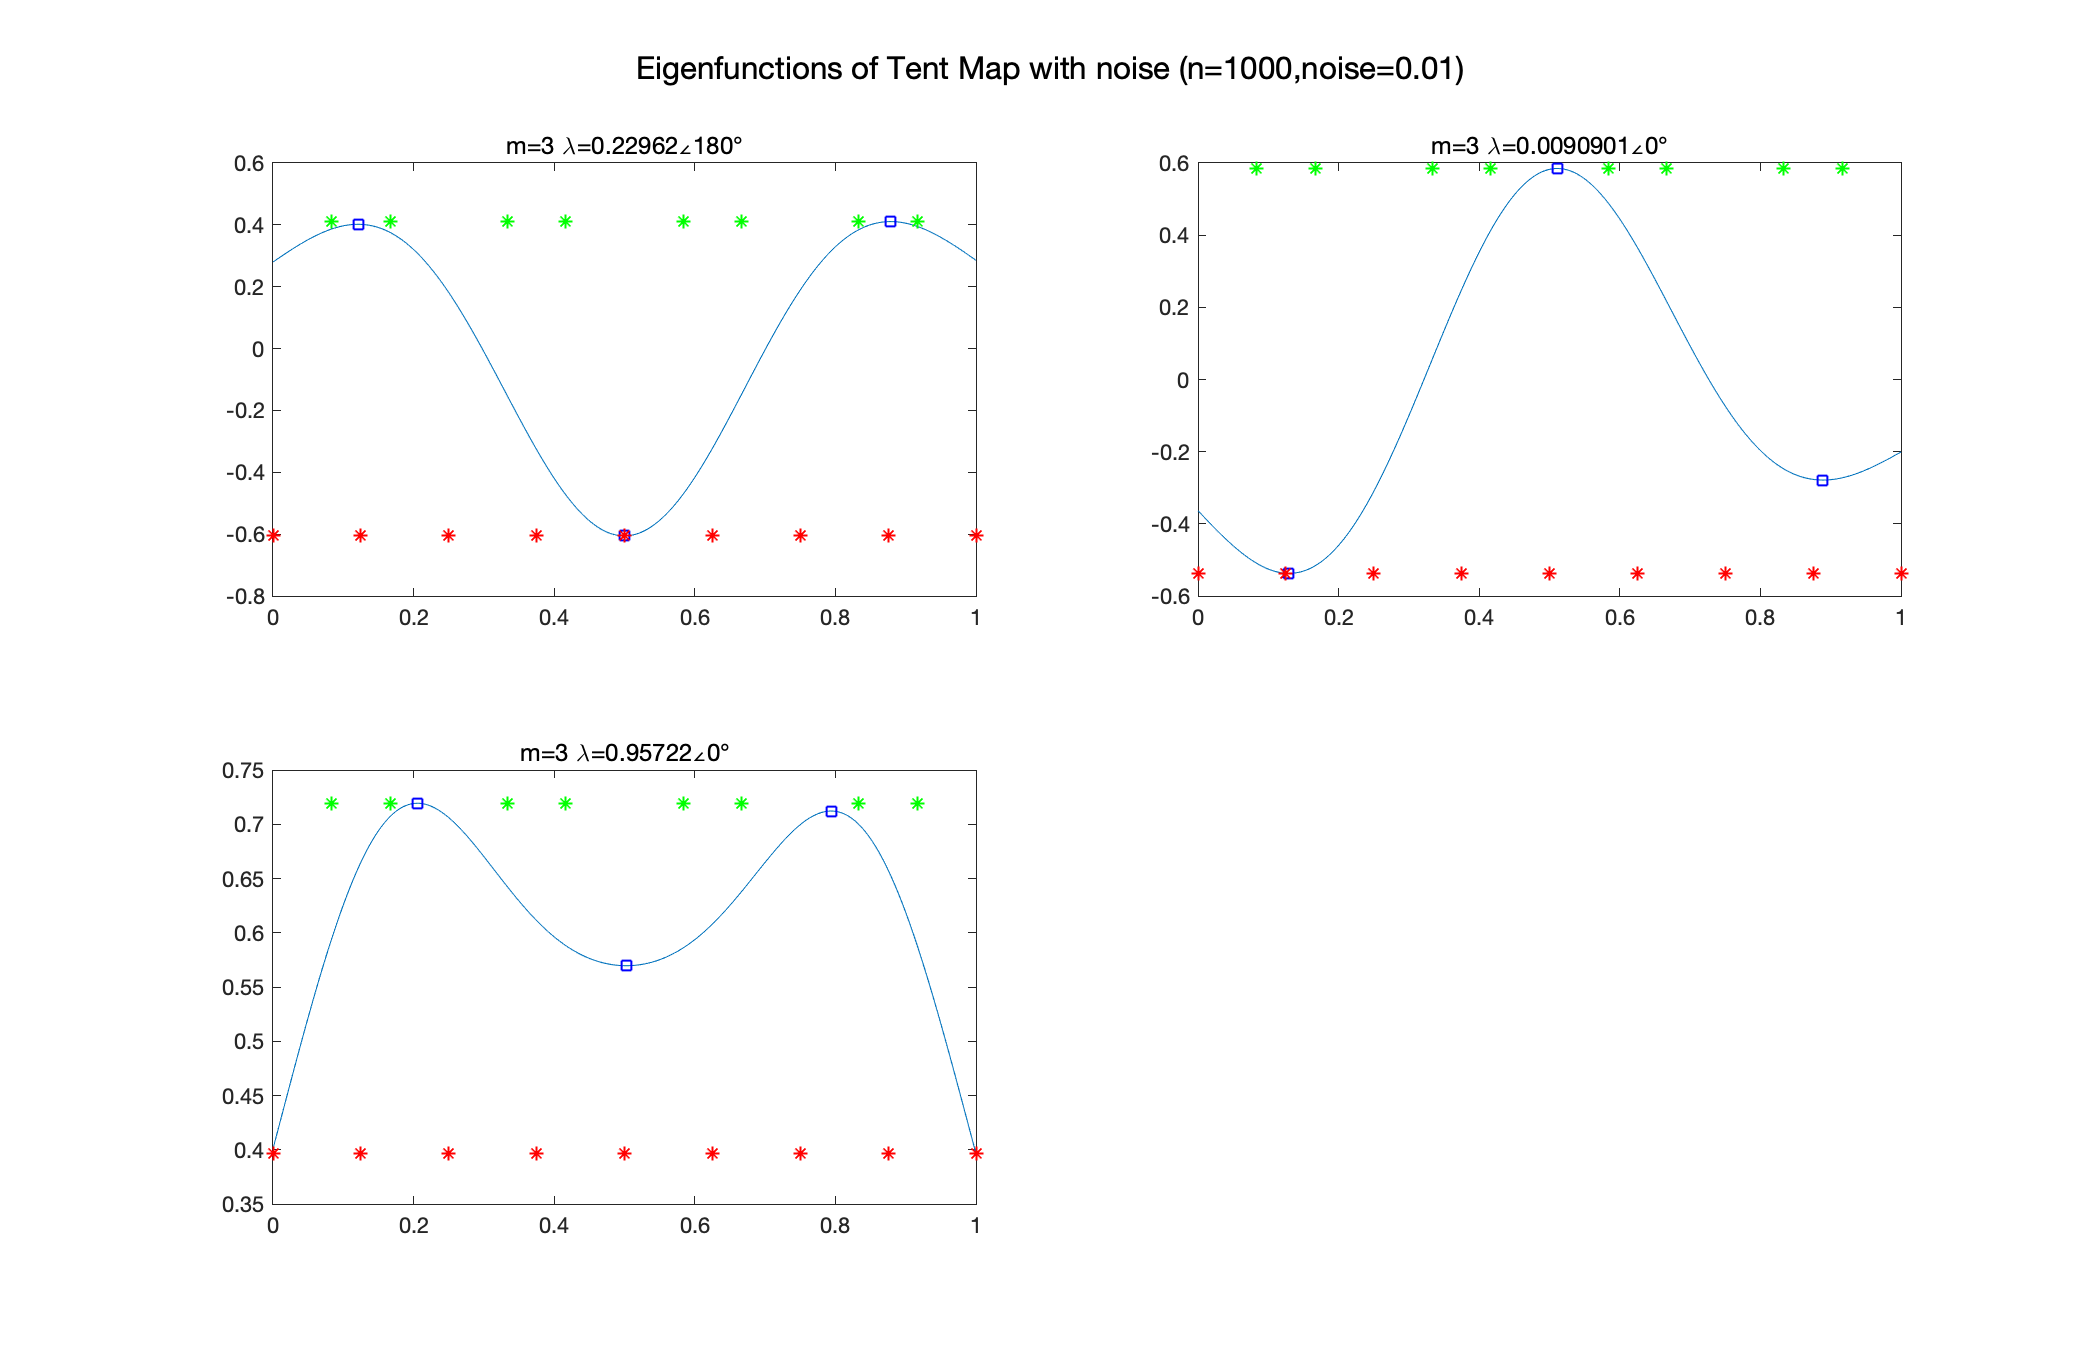
\includegraphics[scale=0.2]{tent/noise/Tent_eigen_noise_n1000m3d0-01}}
    \\
  \subfloat[m=4]{
    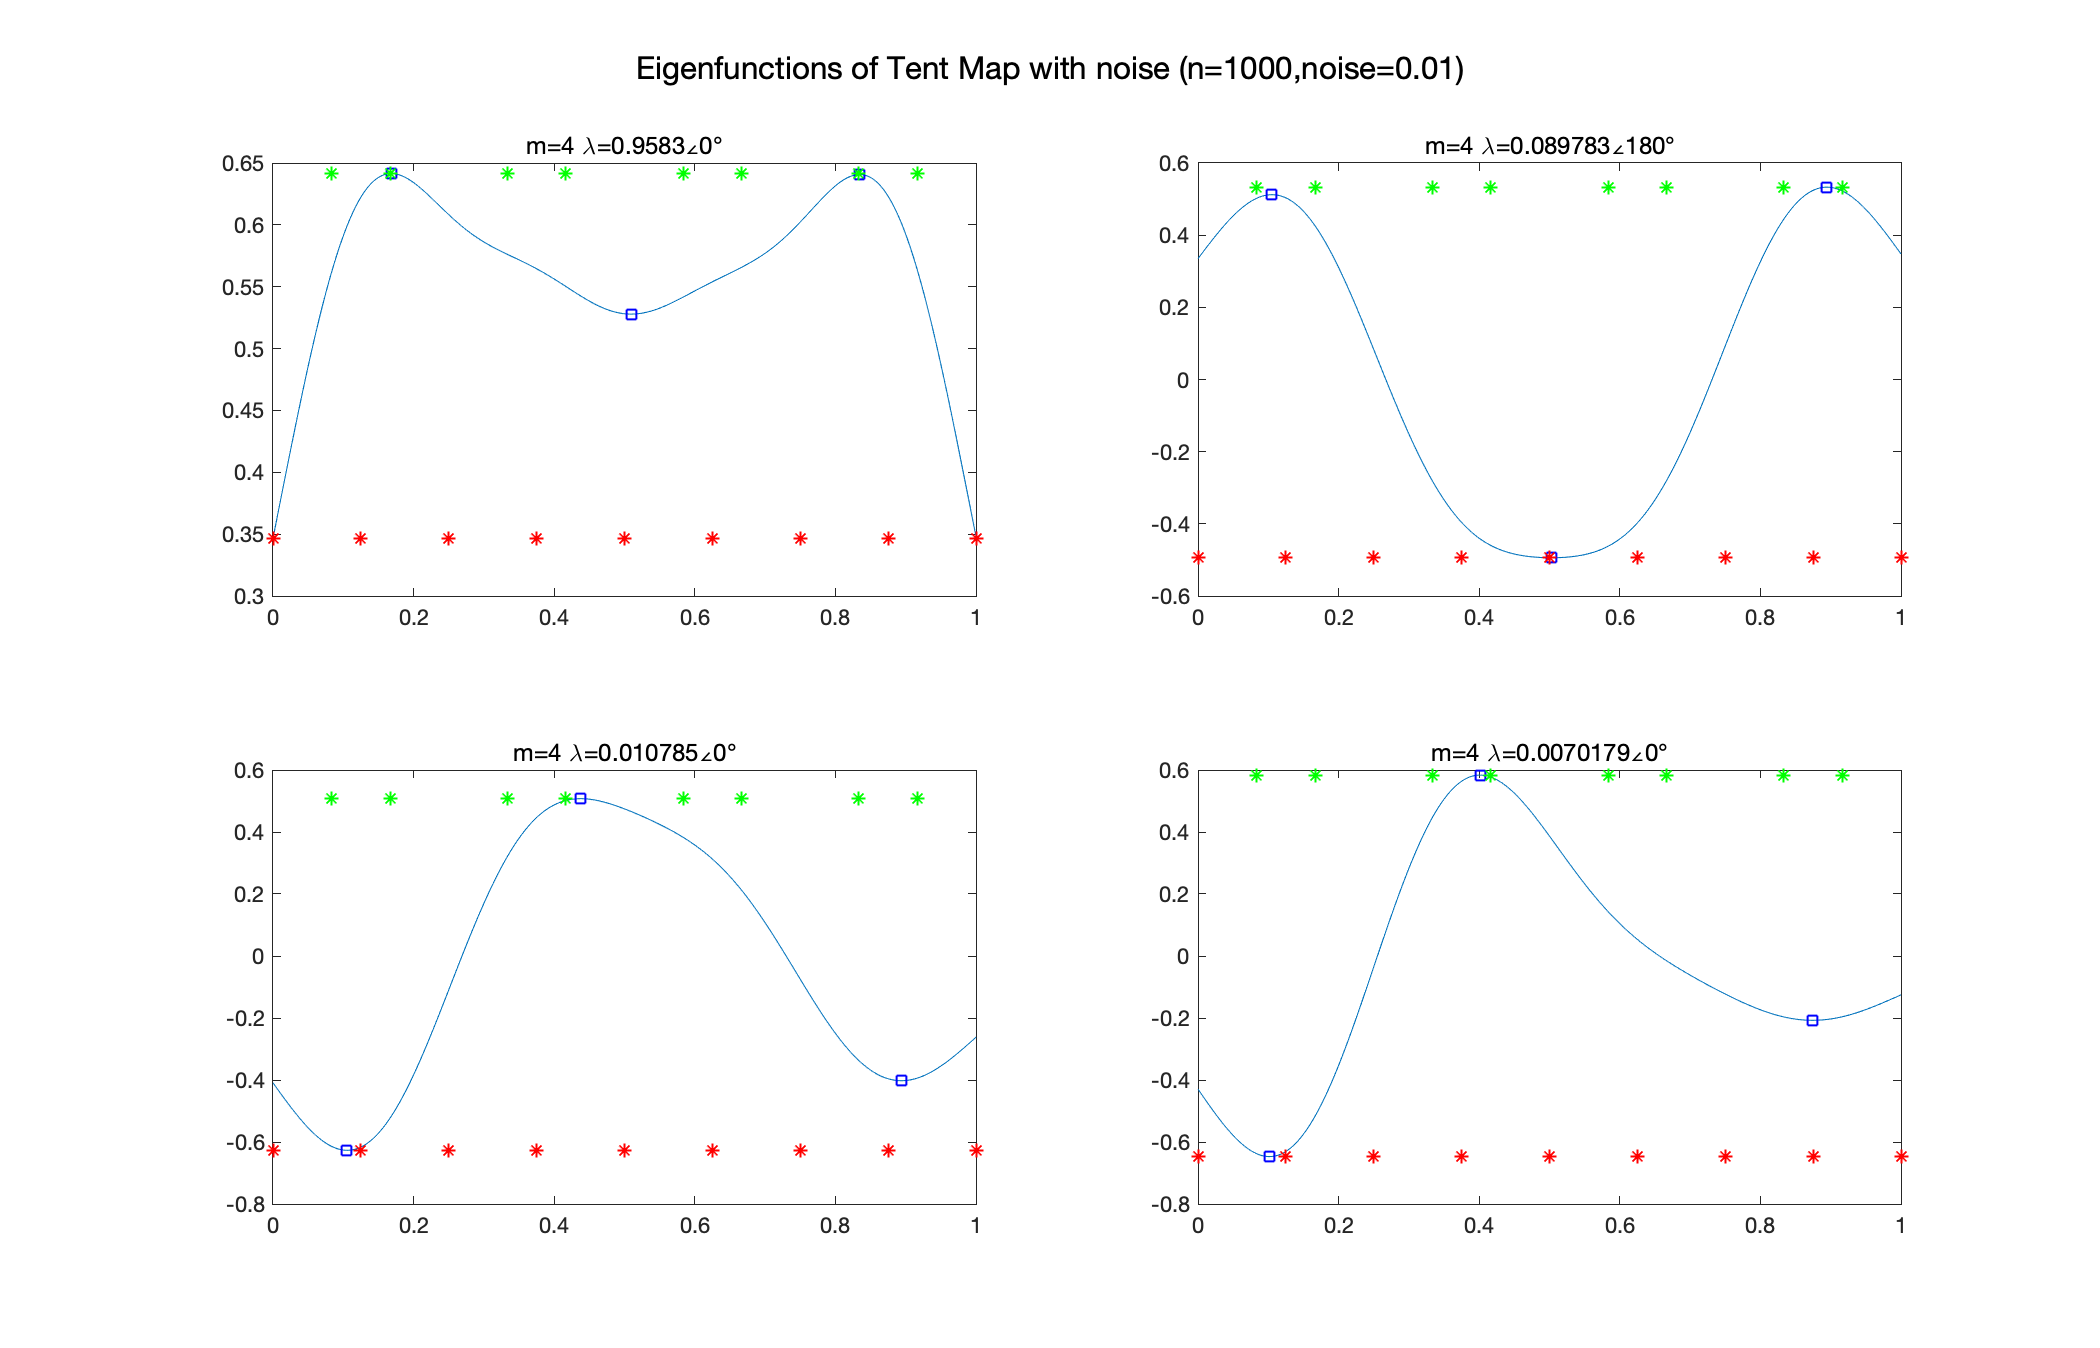
\includegraphics[scale=0.2]{tent/noise/Tent_eigen_noise_n1000m4d0-01}}
  \subfloat[m=5]{
    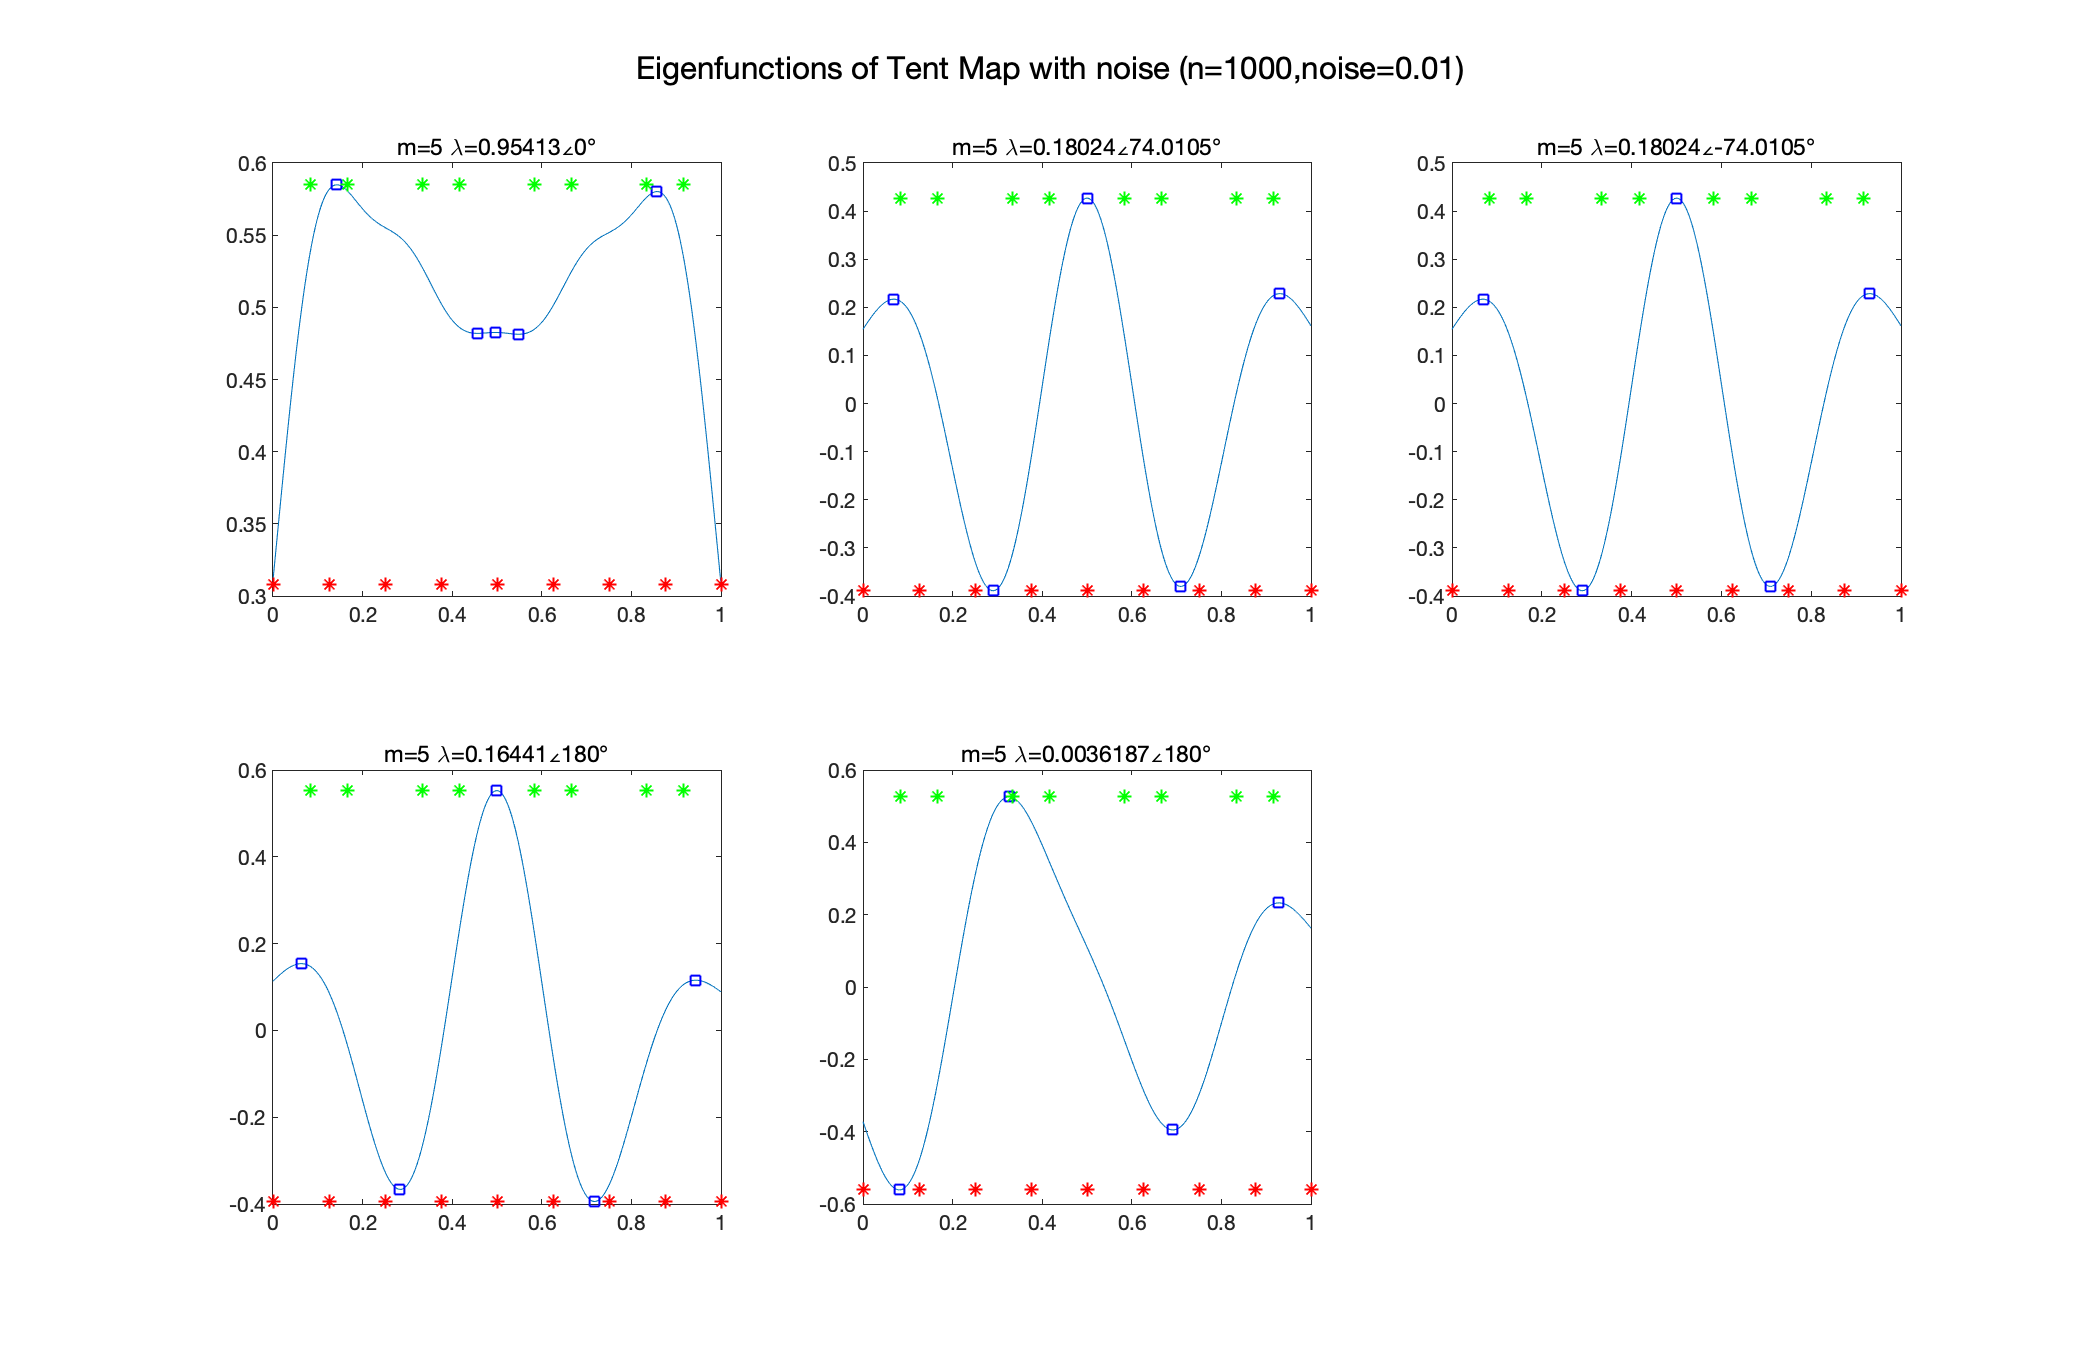
\includegraphics[scale=0.2]{tent/noise/Tent_eigen_noise_n1000m5d0-01}}
    \\
  \subfloat[m=8]{
    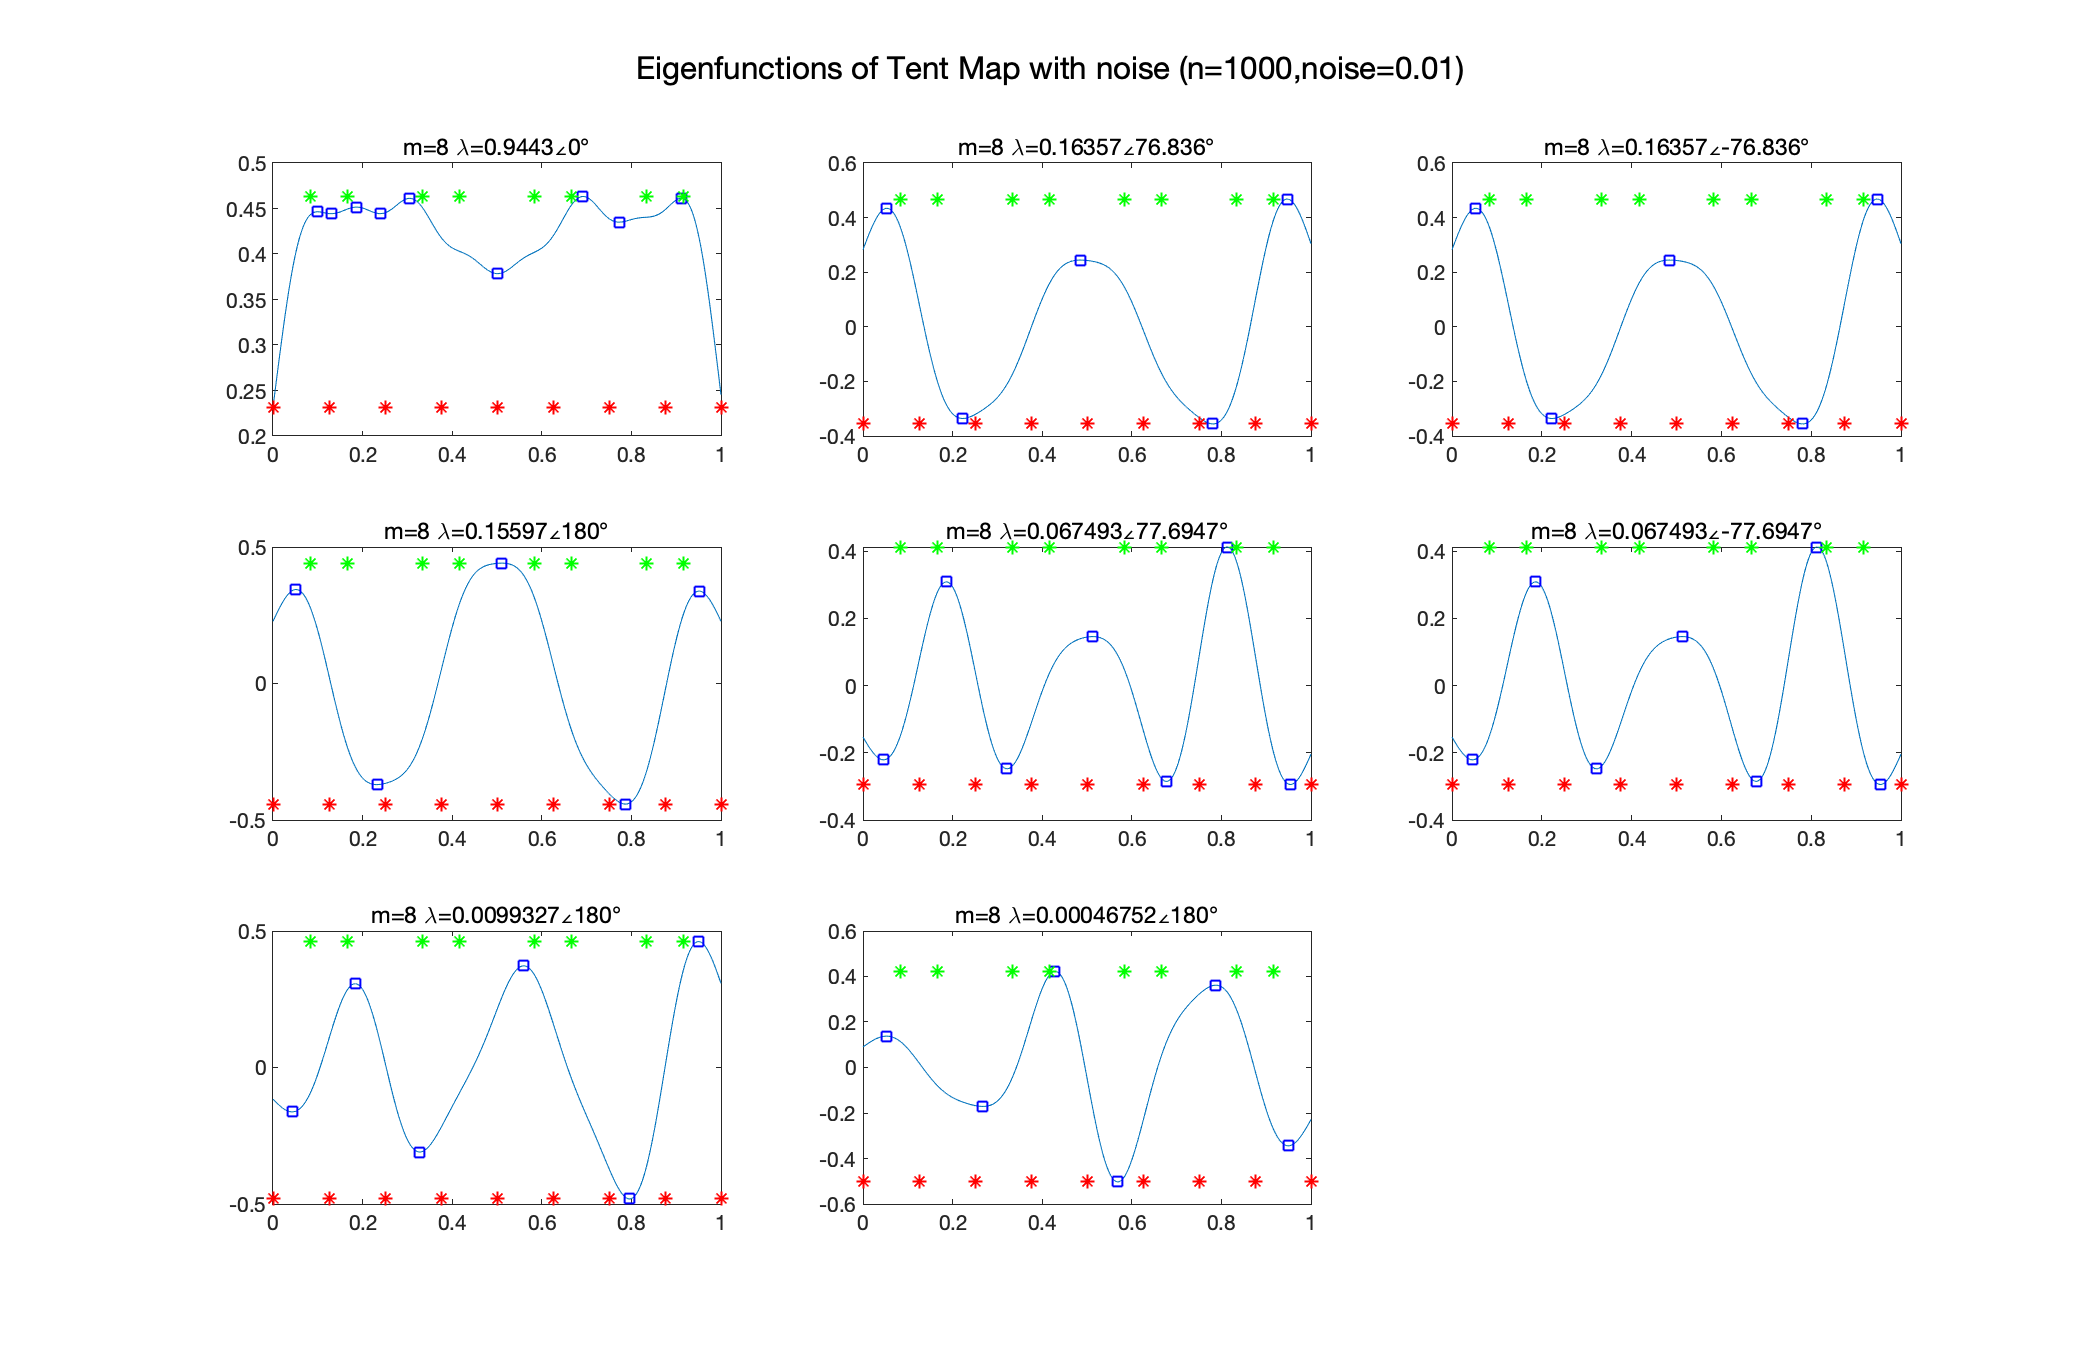
\includegraphics[scale=0.2]{tent/noise/Tent_eigen_noise_n1000m8d0-01}}
  \subfloat[m=10]{
    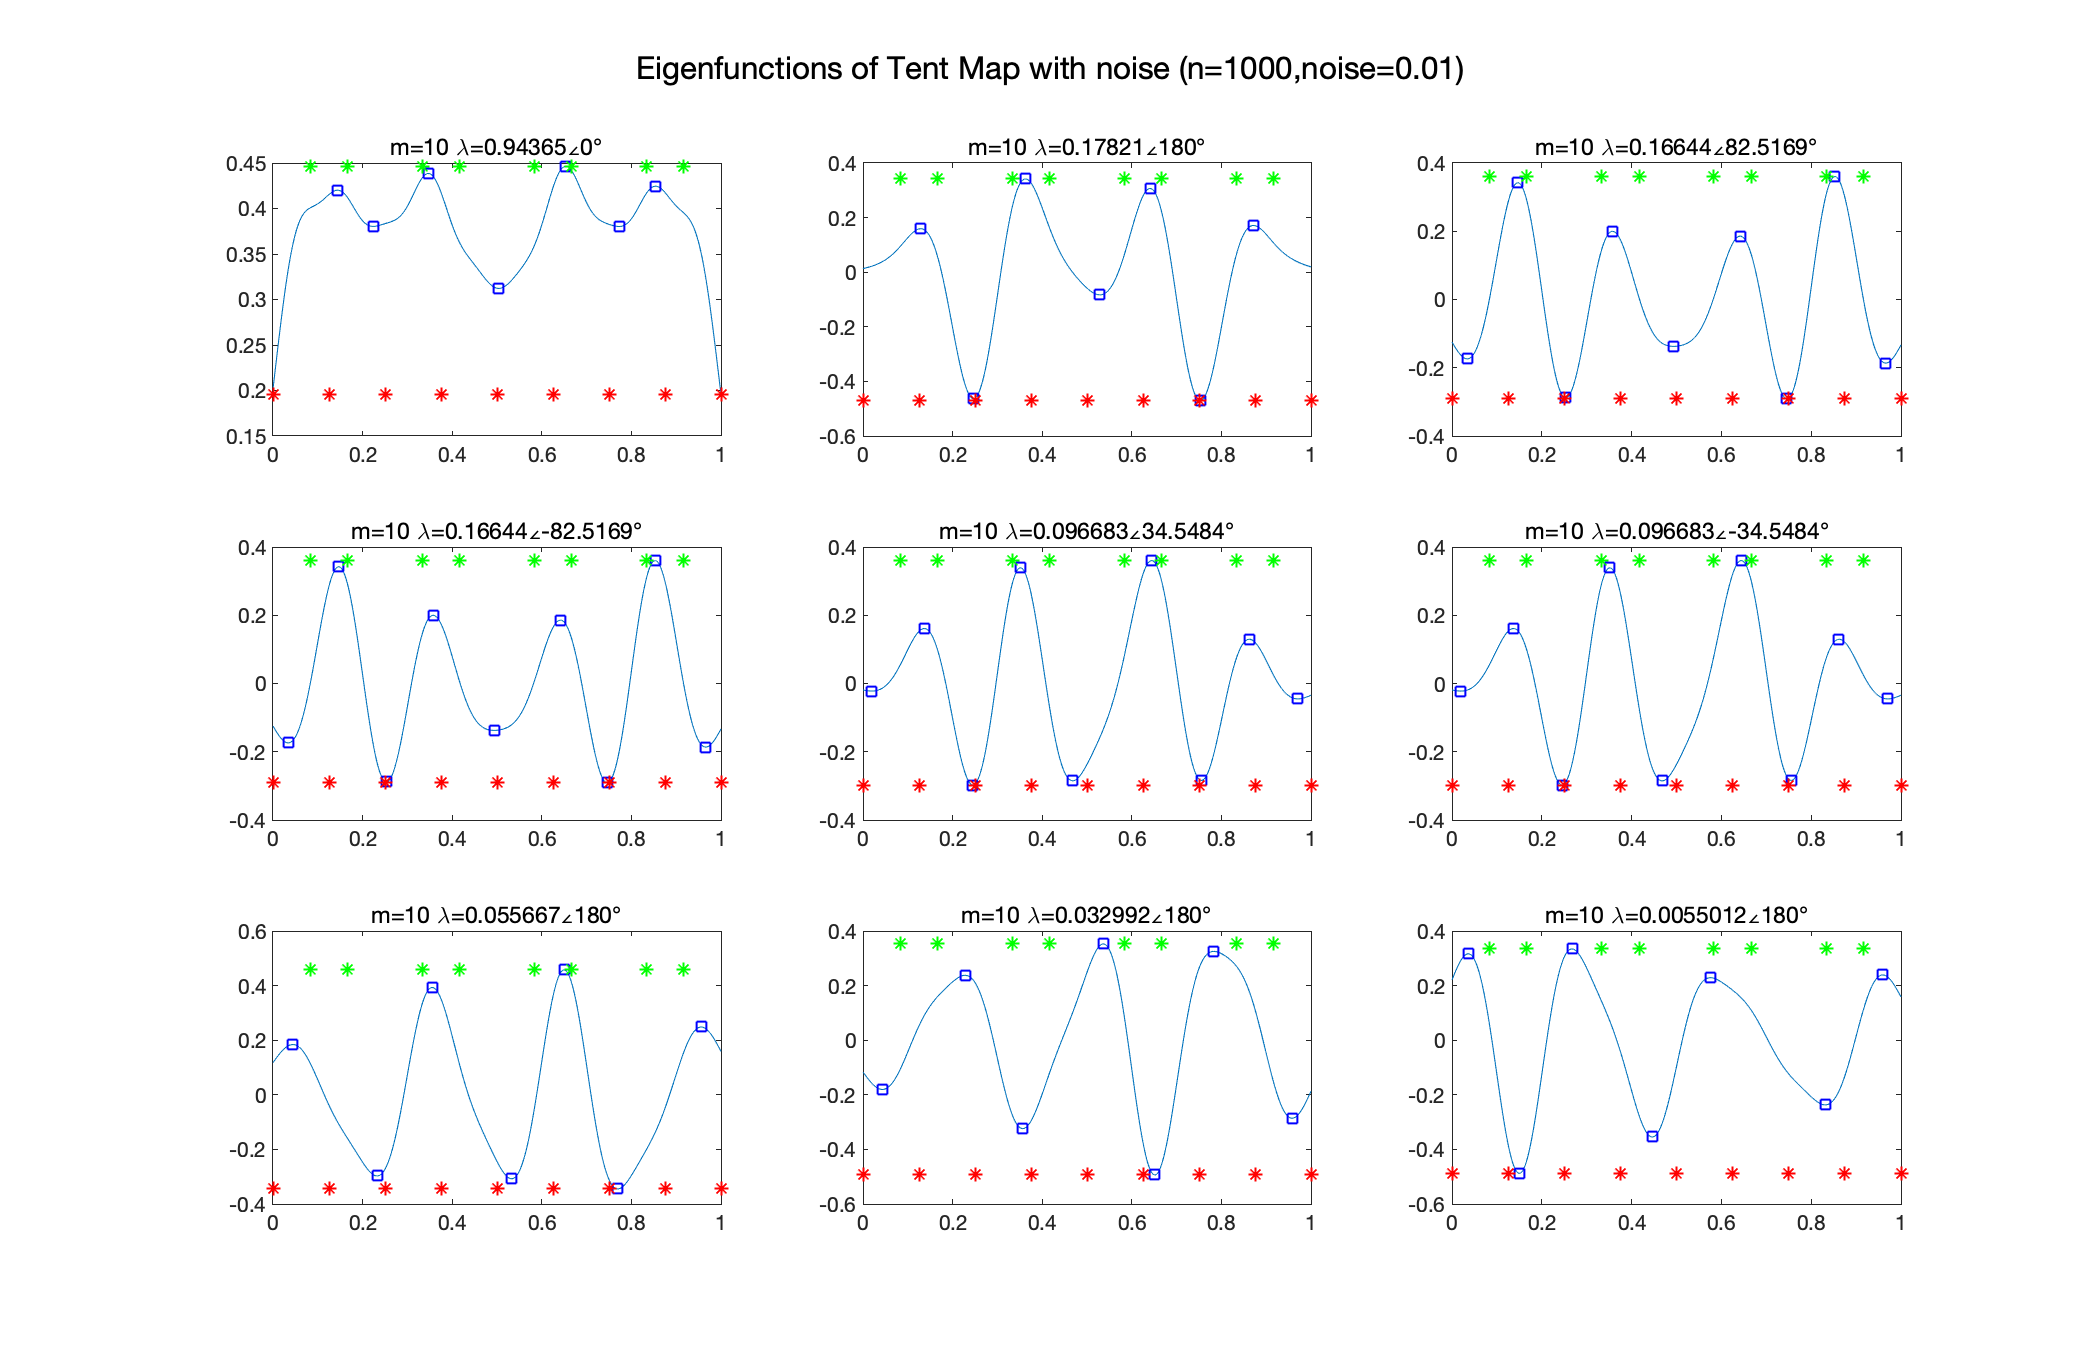
\includegraphics[scale=0.2]{tent/noise/Tent_eigen_noise_n1000m10d0-01}}
    \\
  \subfloat[m=15]{
    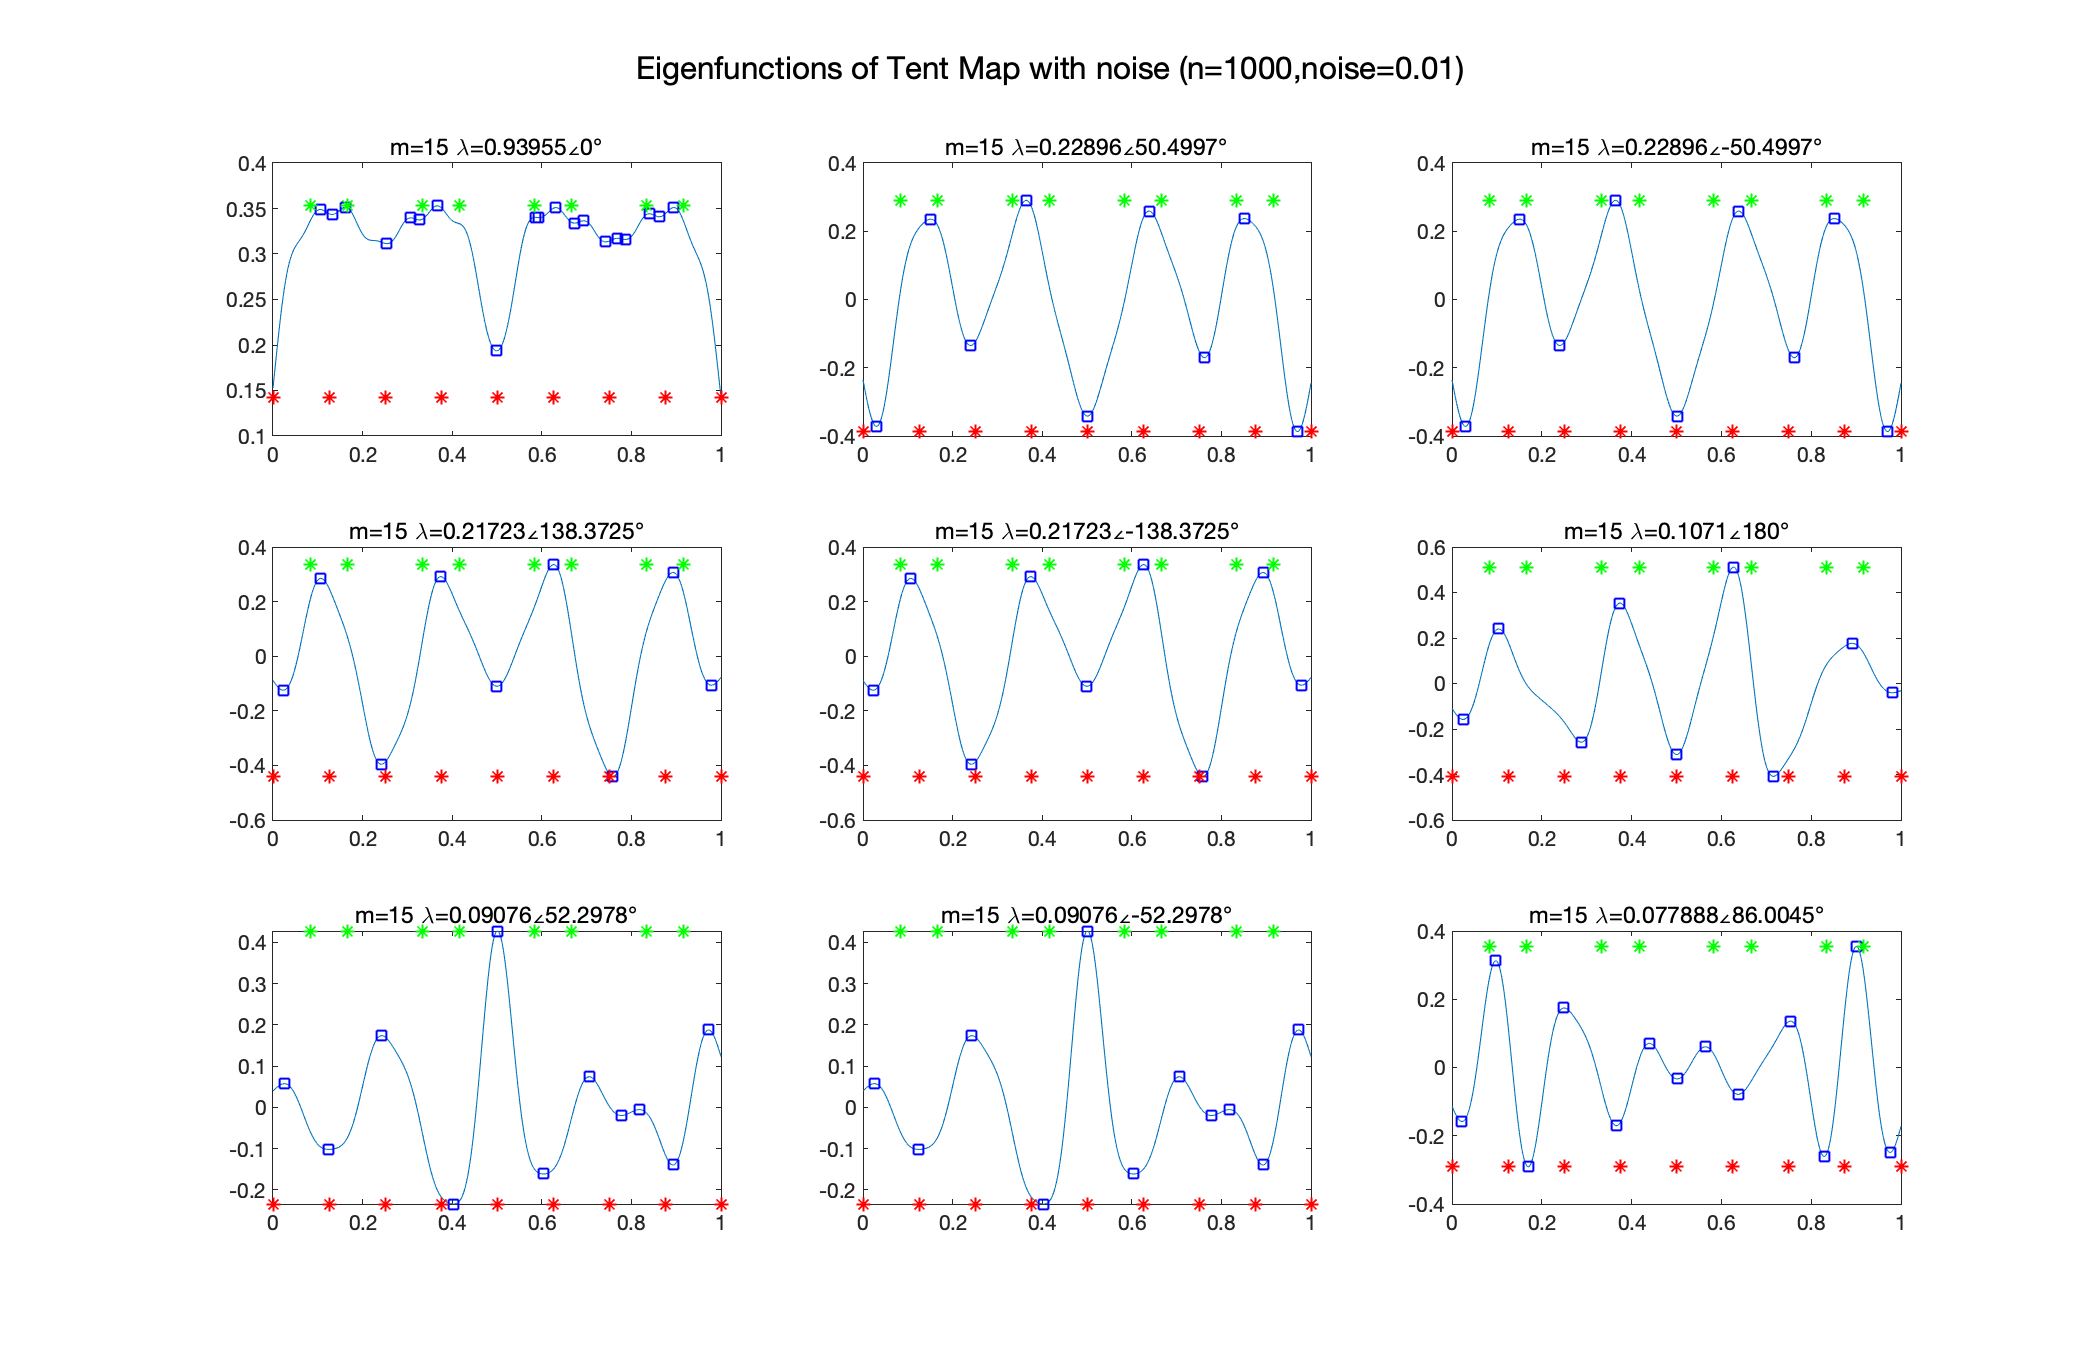
\includegraphics[scale=0.2]{tent/noise/Tent_eigen_noise_n1000m15d0-01}}
  \subfloat[m=20]{
    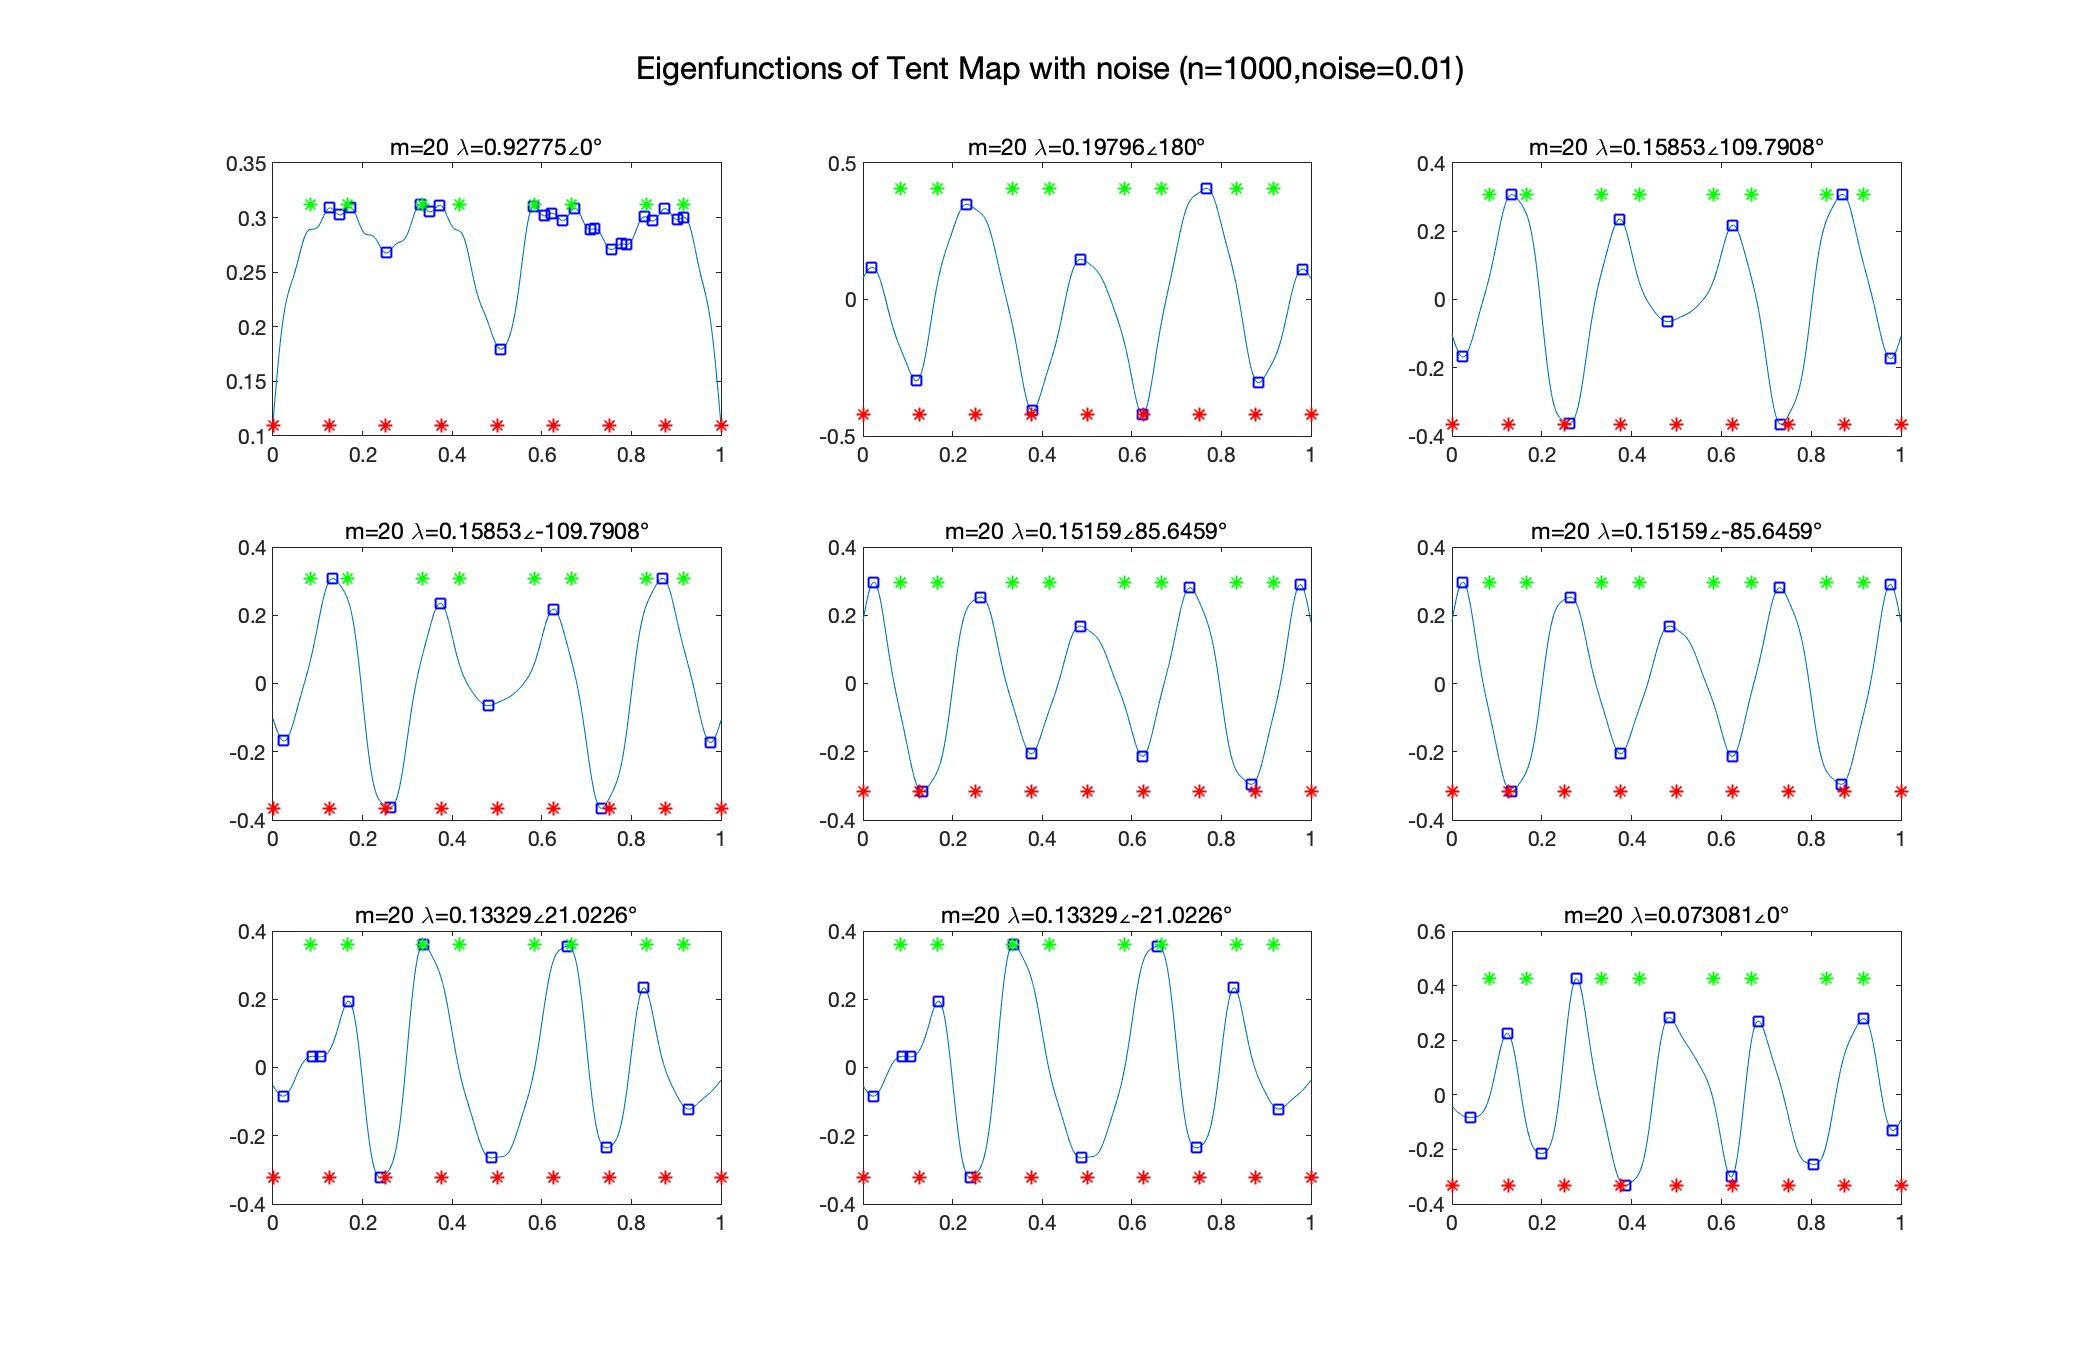
\includegraphics[scale=0.2]{tent/noise/Tent_eigen_noise_n1000m20d0-01}}
    \\
    \caption{帐篷映射的边界点与本征函数($noise=0.01$)}\label{fig:Tent_eigen_noise_n1000m20d0-01}
\end{figure}

在图\ref{fig:Tent_eigen_noise_n1000m20d0-001}(a)第二个小图中,我们观察到由于噪声项的影响,Koopman算符的本征函数的极值点与边界点会有一定距离的偏移,随着基函数数量的增加,本征函数的细节上会有些许变化,但是大致趋势并未发生明显的变化。如图\ref{fig:Tent_eigen_noise_n1000m20d0-001}(h)第七个小图中,本征函数在$x=\frac{1}{2}$处的极值点与边界点发生了稍稍的偏离,但是总体观察其他的几个小图,还是能较好的反映帐篷映射的边界点。图\ref{fig:Tent_eigen_noise_n1000m20d0-01}中增加了噪声的大小$noise=0.01$,本征函数图像变得更不规则了,但总体观察Koopman算符本征函数的极值点,其噪声对其划分边界点的影响并不大。如在图\ref{fig:Tent_eigen_noise_n1000m20d0-01}(h)第一个小图中,本征函数的细节变的稍稍不规则,但是在边界点$x=\frac{1}{2}$附近处同样存在较明显的本征函数极值点。

综上我们可以确定,Koopman算符的本征函数的极值点反映了帐篷映射的边界点这一结论是具有鲁棒性的。


\subsubsection{寻找更精确的边界点}
我们已经初步探究了Koopman算符的本征函数的极值点反映了帐篷映射的边界点,并且提出可以通过Koopman算符的极值点来确定边界点,但是其精确性则有待进一步讨论,因为数值计算总会有一定的误差,能否在给定误差范围内寻找到我们所需要的边界点变得尤为重要。

在之前的探究中,我们发现随着基函数数量的增加,本征函数对边界点的刻画更为精细:函数格点数量越多,本征函数描述的边界点的层次与精细度随之增加,为了验证我们的这个结论,我们进行如下对比:当基函数数量增加一倍时,探究本征函数的极值点之间的关系。由于不同基函数数量下的本征值较多,我们需要选取合适的本征函数,为此我们需要寻找不同基函数数量下反映同样动力学特征的本征函数,我们可以利用互相关函数来定义本征函数之间的相似性(式\ref{equ:cov_xy}):
\begin{equation}
  cov(X,Y)=\dfrac{\sum_{i=1}^{n}(X_i-\overline{X})(Y_i-\overline{Y})}{n-1}
  \label{equ:cov_xy}
\end{equation}

为了刻画不同基函数之间的关系,我们可以考虑这样一个问题,对于两个基函数数量$m_1$和$m_2$,若我们已知$m_1$下的本征函数,能够通过本征函数的定义来得到$m_2$下的本征函数?这转化为一个求函数最小值对应的参数问题,用数学公式描述为式\ref{equ:argmin}:
\begin{equation}
  \mathop{\arg\min}_{\boldsymbol{\phi_{m_2}}} \ \ || U\phi_{m_2}-\lambda \phi_{m_2} || + \mu ||corr(\phi_{m_1},\phi_{m_2})||
  \label{equ:argmin}
\end{equation}
其中第一项为满足本征函数的条件项,第二项为满足具有相关性的对应$m_1$和$m_2$的本征函数。且第二项的系数应远小于第一项(满足本征函数定义为主,满足相关系为辅),同时我们应有约束$||\phi_{m_2}||=1$。在此条件下,我们探究不同基函数数量下本征函数之间的关系。

在图\ref{fig:Tent_findeigen_m8m16}中,我们根据寻找函数式\ref{equ:argmin}最小值进行了四组对比:$m=8,16$,$m=16,32$,$m=32,64$,$m=64,128$,在每个图中,蓝色的线表示较小的基函数数量下的本征函数,我们以此蓝色的本征函数$\phi_{m_1}$为基础,根据式\ref{equ:argmin}计算得到较大的基函数数量下的本征函数,即红色的本征函数$\phi_{m_2}$。

\begin{figure}[!]
  \centering
  \subfloat[m=8,16]{
    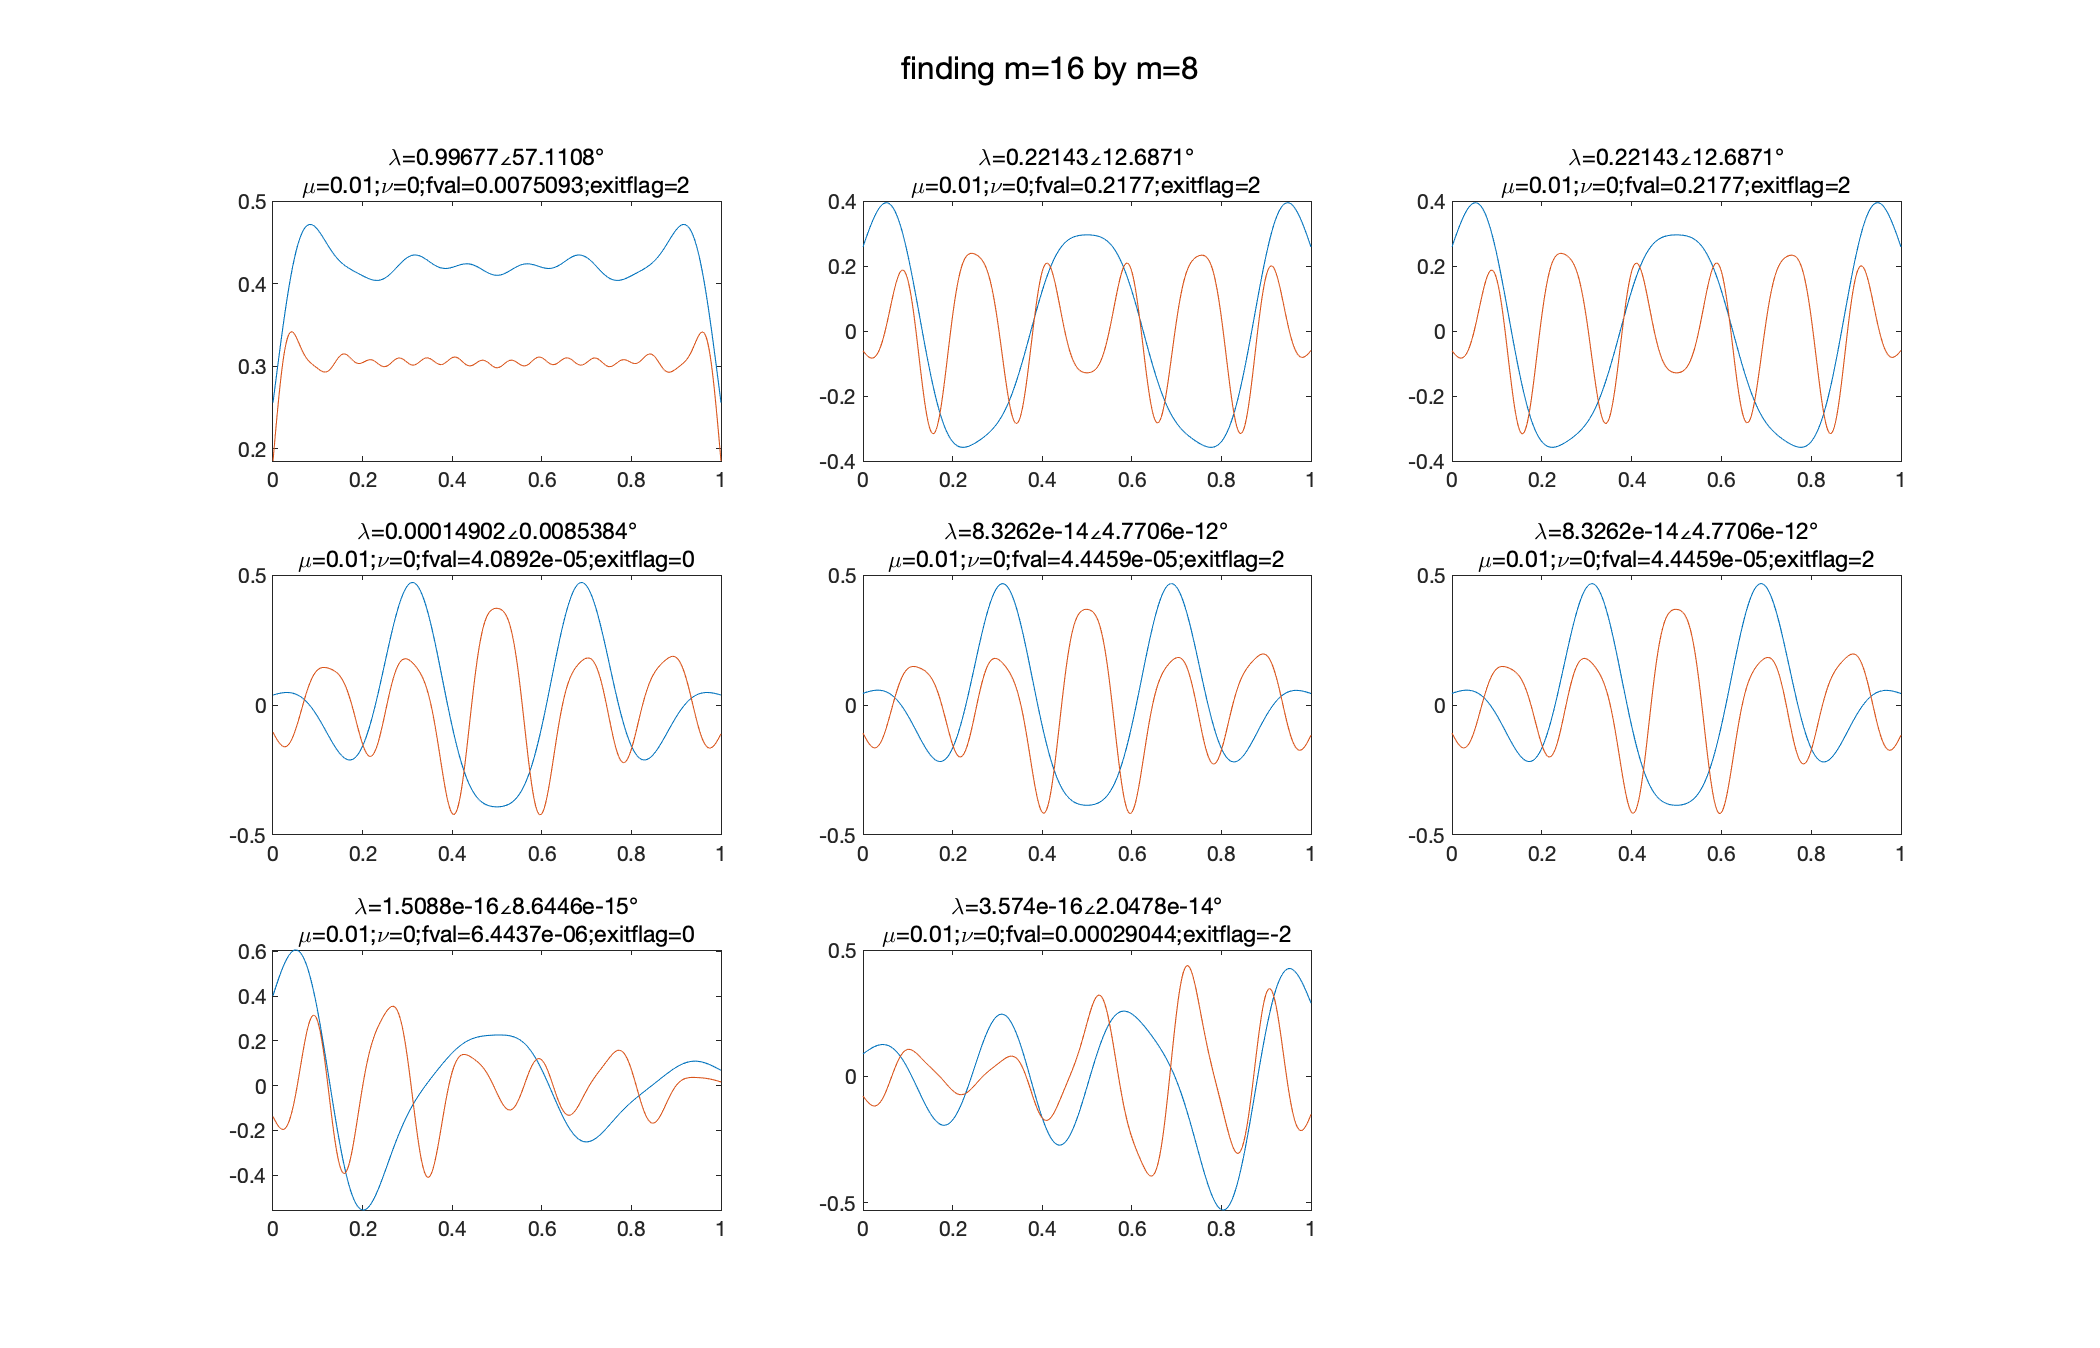
\includegraphics[scale=0.2]{tent/accurate/Tent_findeigen_m8m16}}
  \subfloat[m=16,32]{
    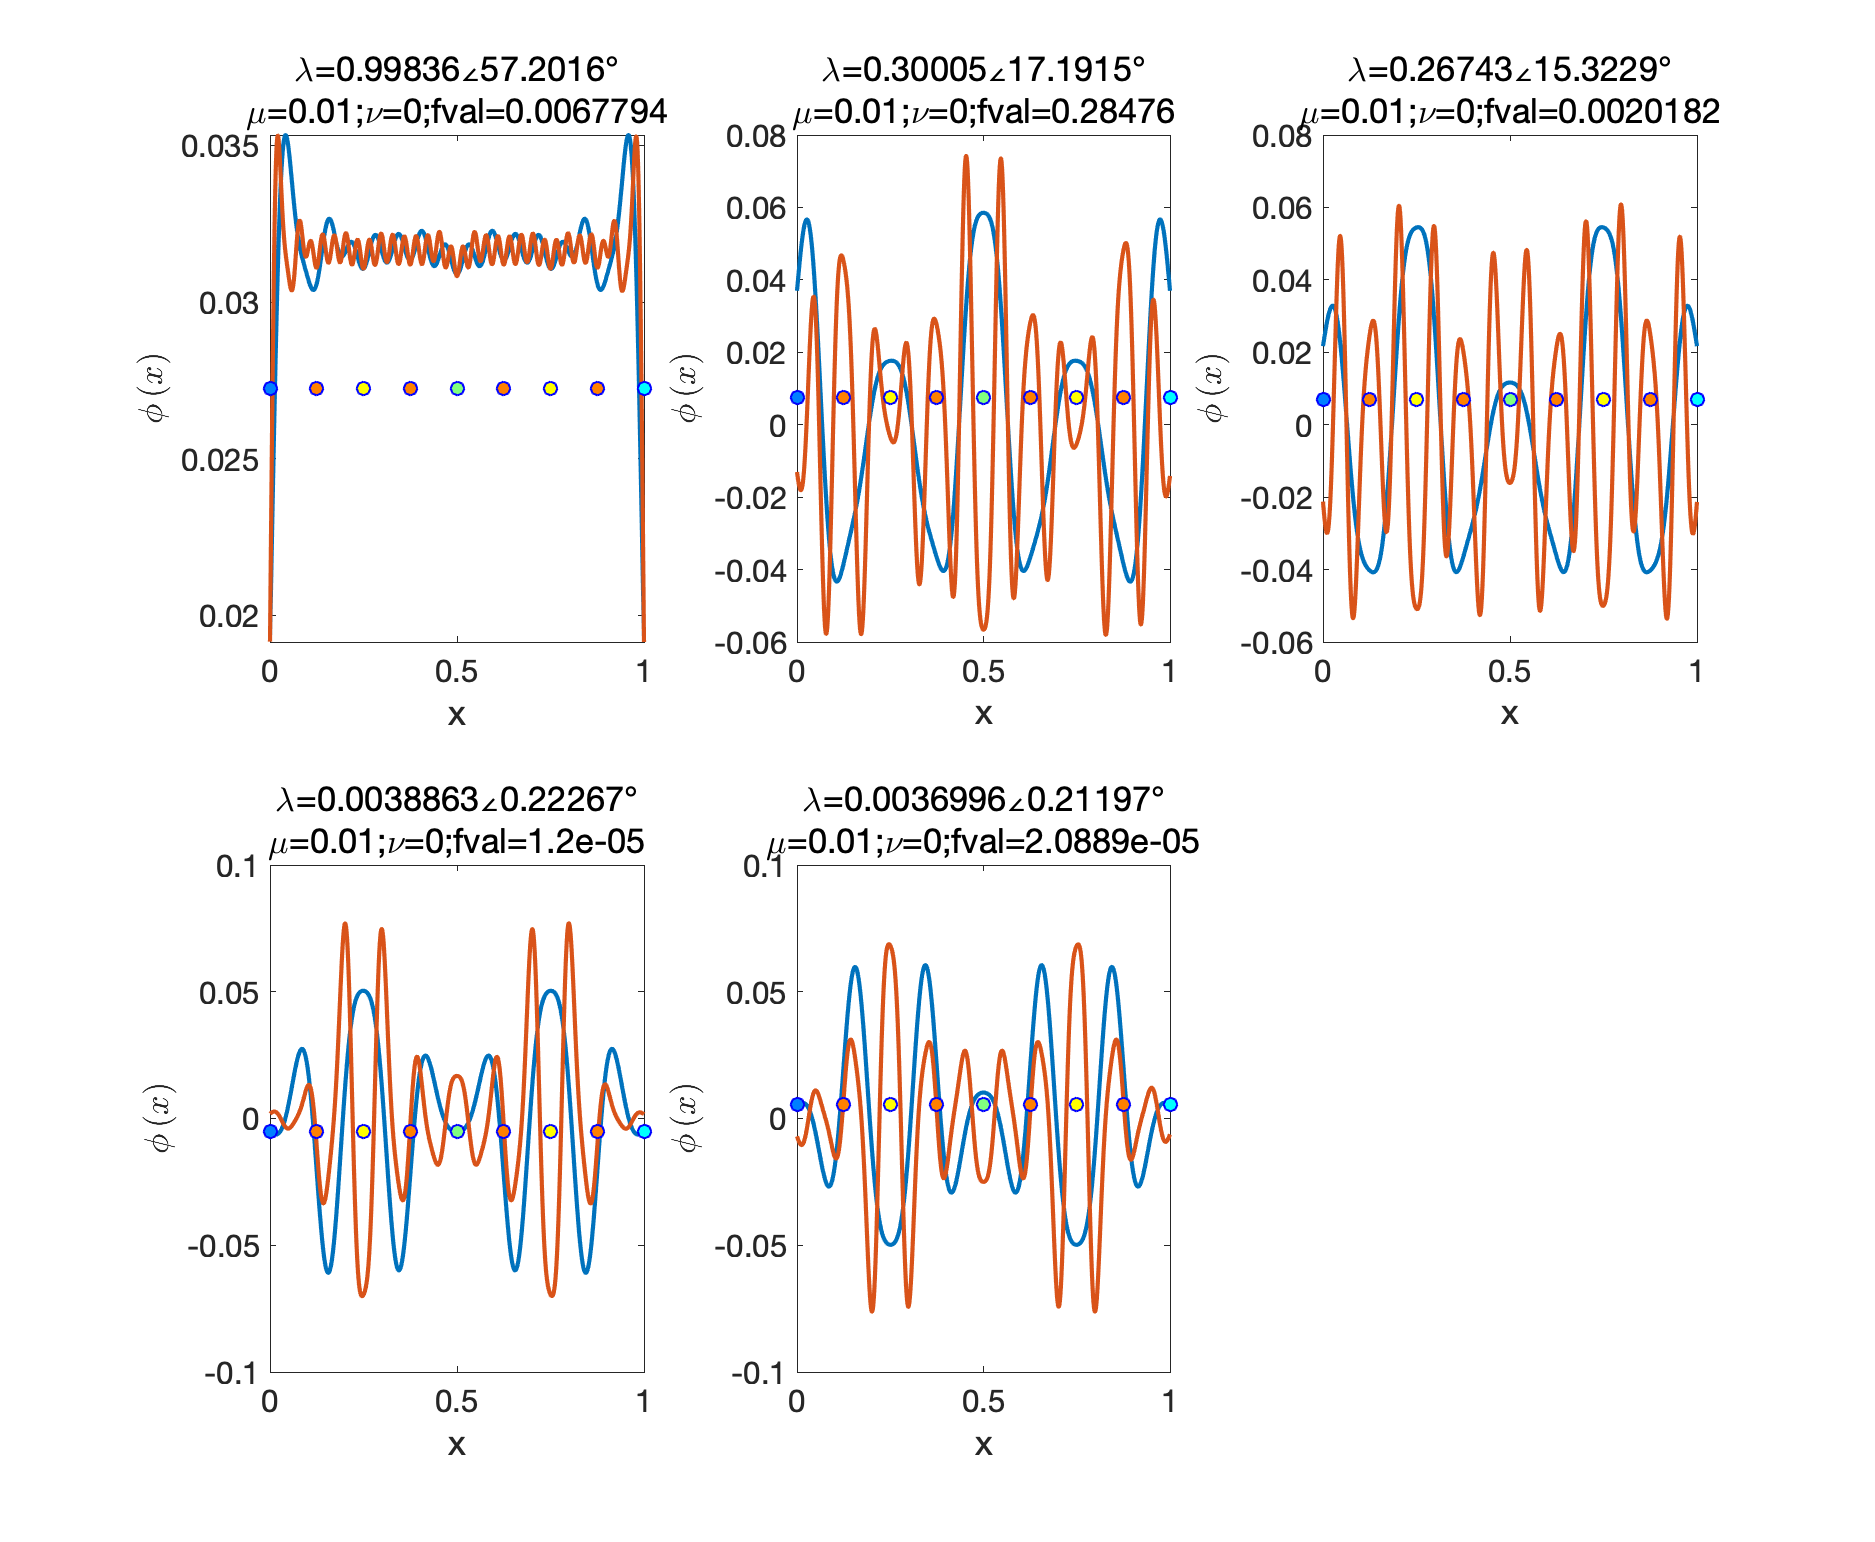
\includegraphics[scale=0.2]{tent/accurate/Tent_findeigen_m16m32}}
    \\
  \subfloat[m=32,64]{
    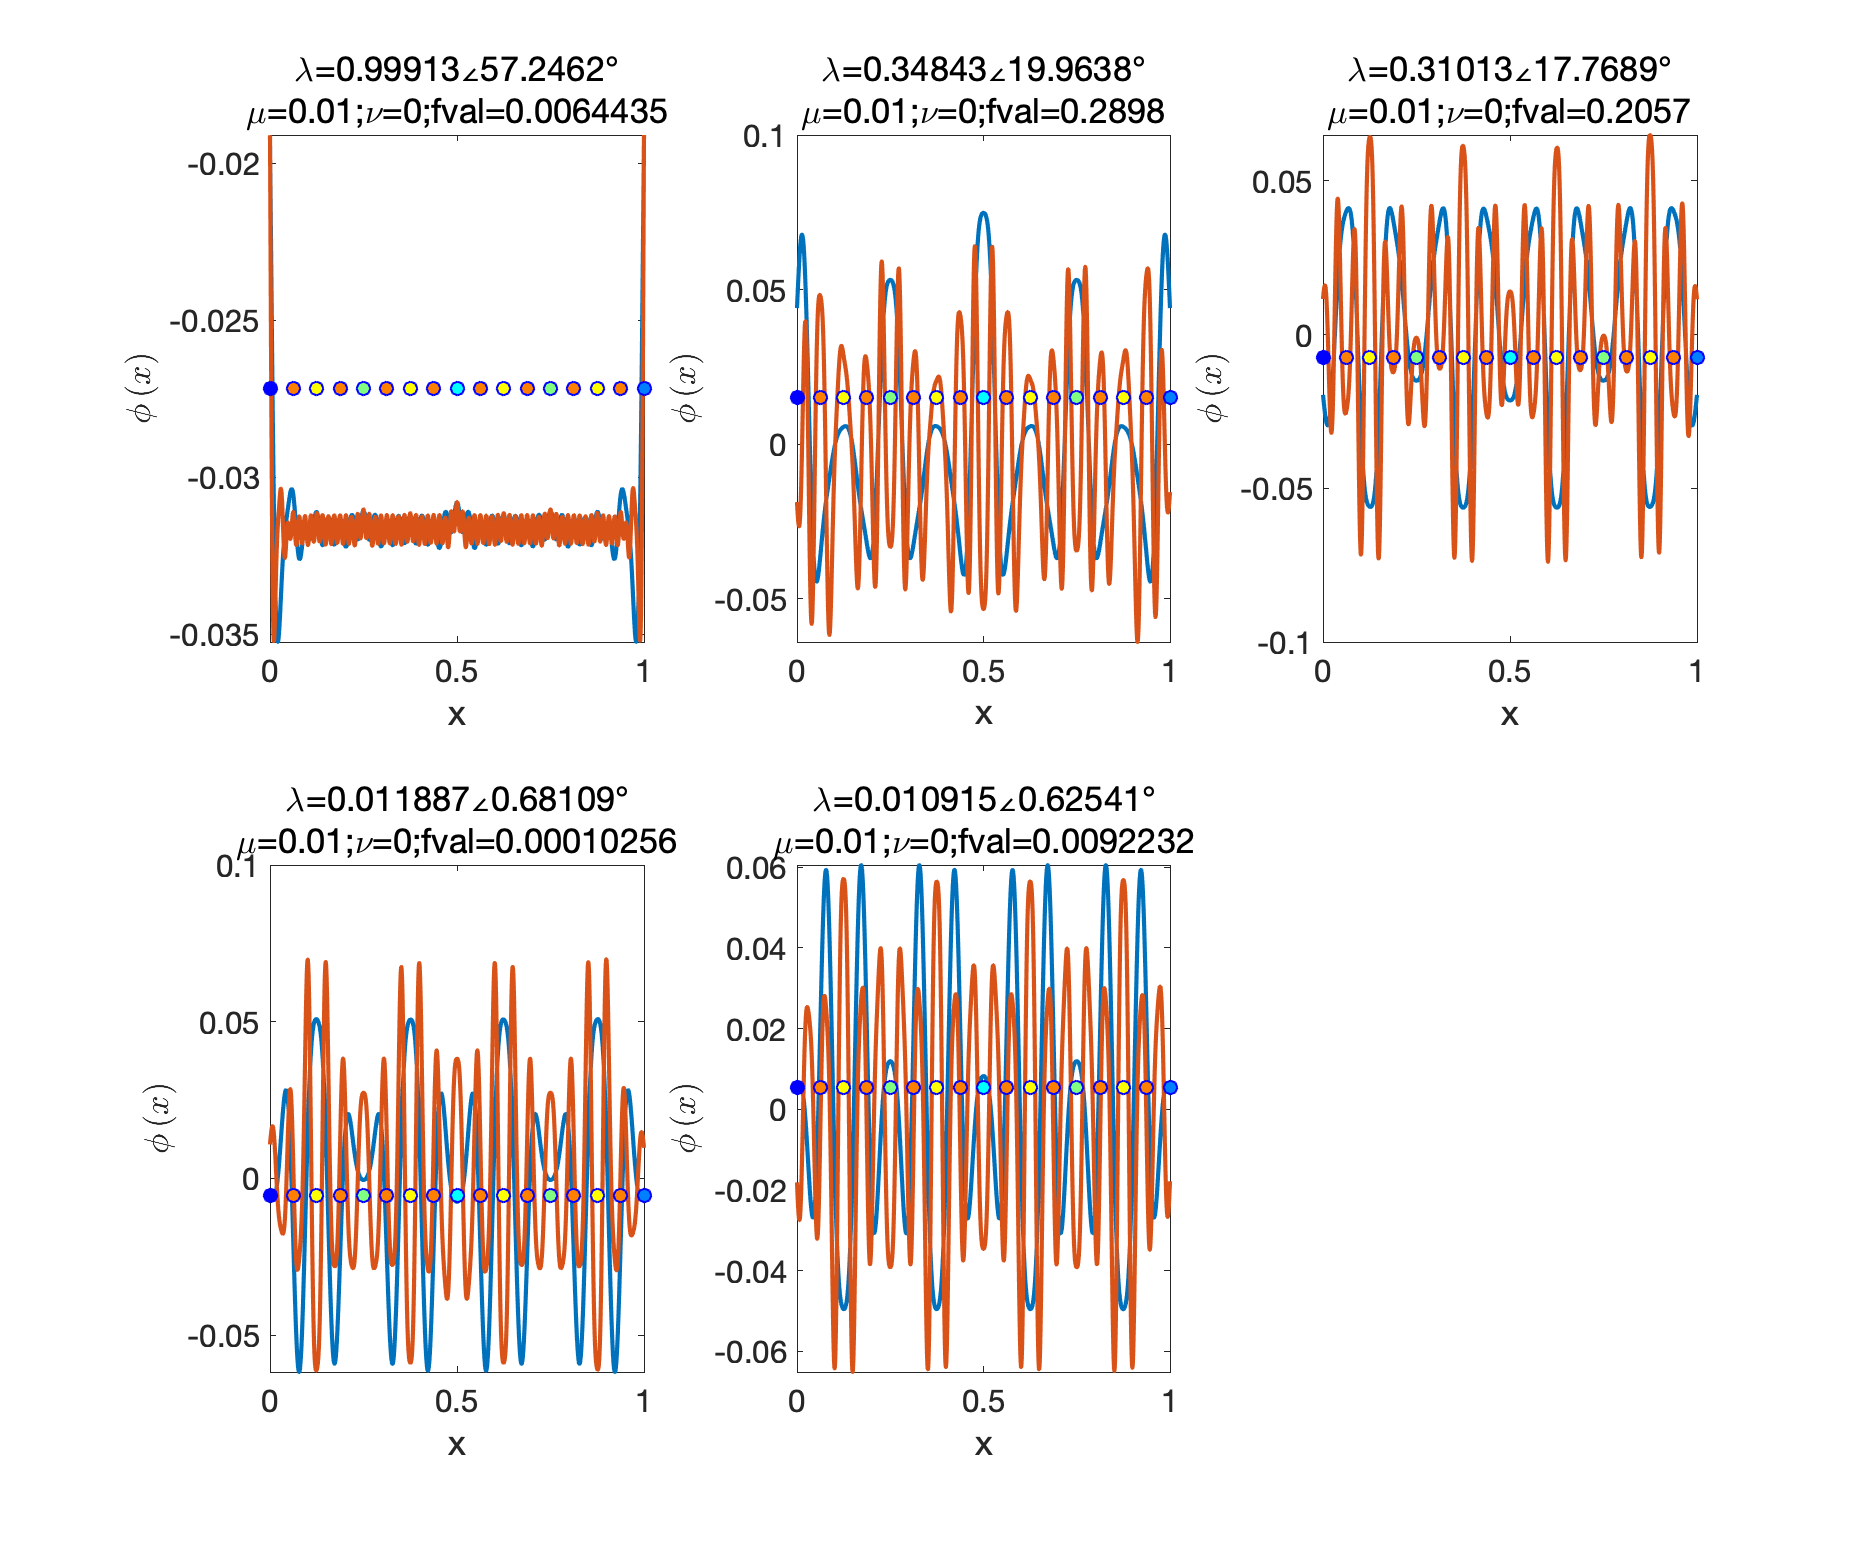
\includegraphics[scale=0.2]{tent/accurate/Tent_findeigen_m32m64}}
  \subfloat[m=64,128]{
    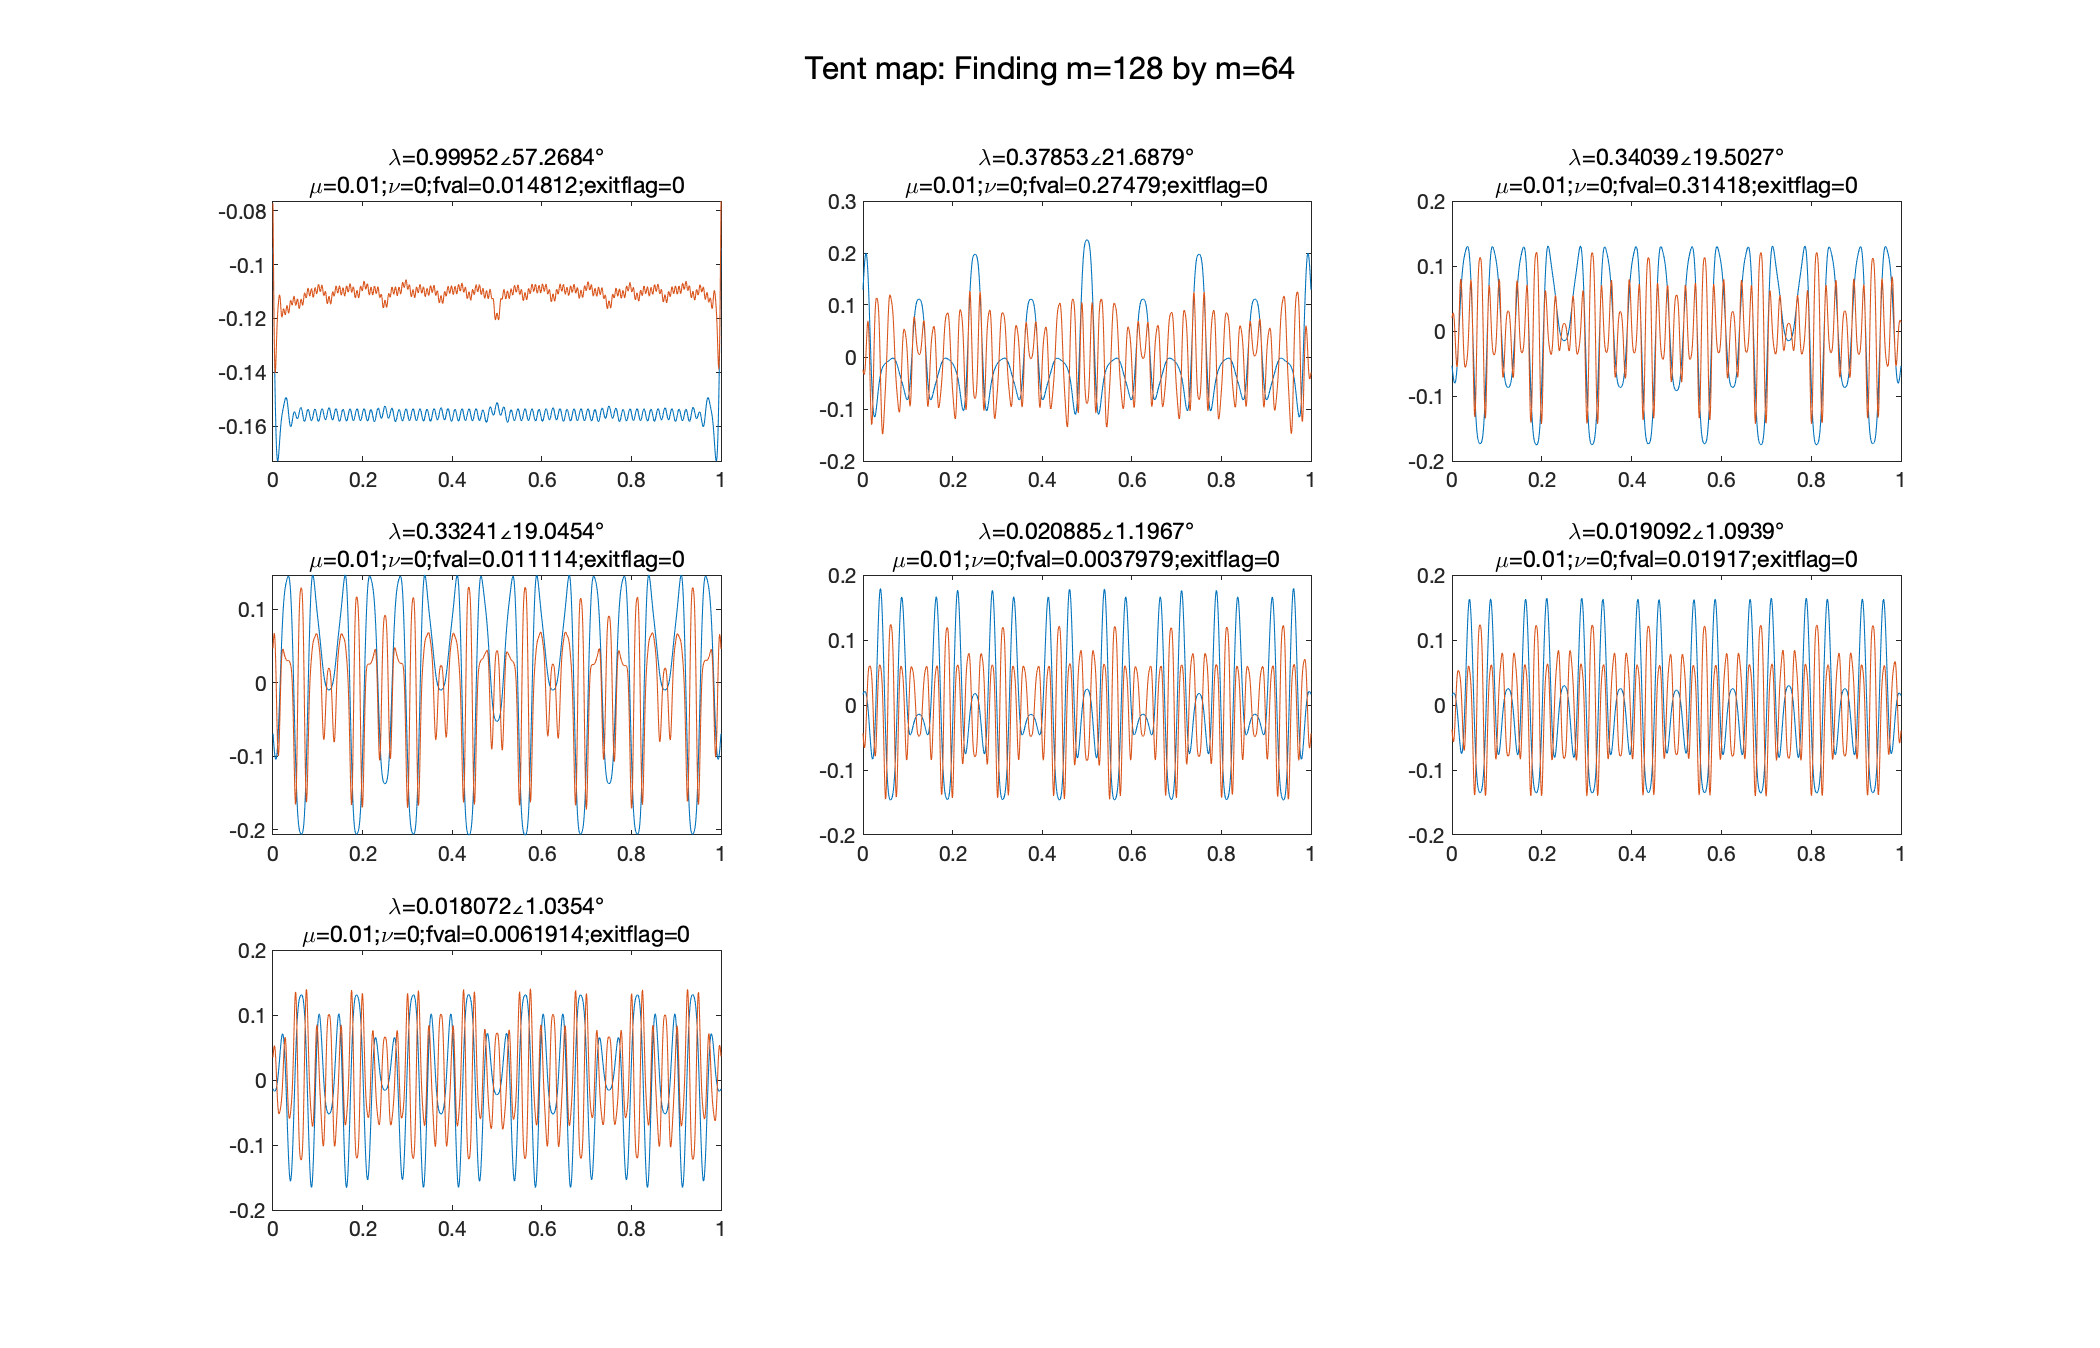
\includegraphics[scale=0.2]{tent/accurate/Tent_findeigen_m64m128}}
    \\
  \caption[帐篷映射本征函数不同基函数数量之间的对应关系]{帐篷映射本征函数不同基函数数量之间的对应关系($n=1000$):根据较小基函数数量的本征函数(蓝色)寻找满足条件的较大基函数数量的本征函数(红色)}\label{fig:Tent_findeigen_m8m16}
\end{figure}

在图\ref{fig:Tent_findeigen_m8m16}(b)第一个小图中,我们发现两个本征函数的分布几乎相同,这是由于我们在计算函数最小值时第二项的因素造成的,但在图\ref{fig:Tent_findeigen_m8m16}(b)第二个小图中,随着基函数数量扩大一倍,本征函数的极值点的数量也增加了一倍左右,且红色本征值的极值点并未丢失蓝色本征值的极值点,且红色本征值的极值点较蓝色本征值点增加了一些点,通过数据上的验证,我们发现这些多出来的极值点恰好处于某一层次下的帐篷映射的边界点。这说明了随着基函数数量的增加,本征函数描述边界点的层次有所增加,这使得我们扩充了之前的结论:Koopman算符的本征函数的极值点反映了帐篷映射的边界点,且随着函数格点数量的增加,我们对边界点层次的刻画也更为精细。

从理论上来讲,只要我们能够取足够多的基函数数量,便能寻找到足够精细精细的边界点,从而找到足够精细的符号动力学的分界点。此外,这为我们寻找不同层次的边界点提供了一种方法:我们可以通过增加本征函数的数量来不断精确我们对边界点的划分,同时可辅以迭代关系来确定边界点的层次。图\ref{fig:Tent_auto_level_n1000_m4}反映了在不同基函数下通过本征函数极值点及迭代关系确定的边界点的层次。

\begin{figure}[!]
  \centering
  \subfloat[m=4]{
    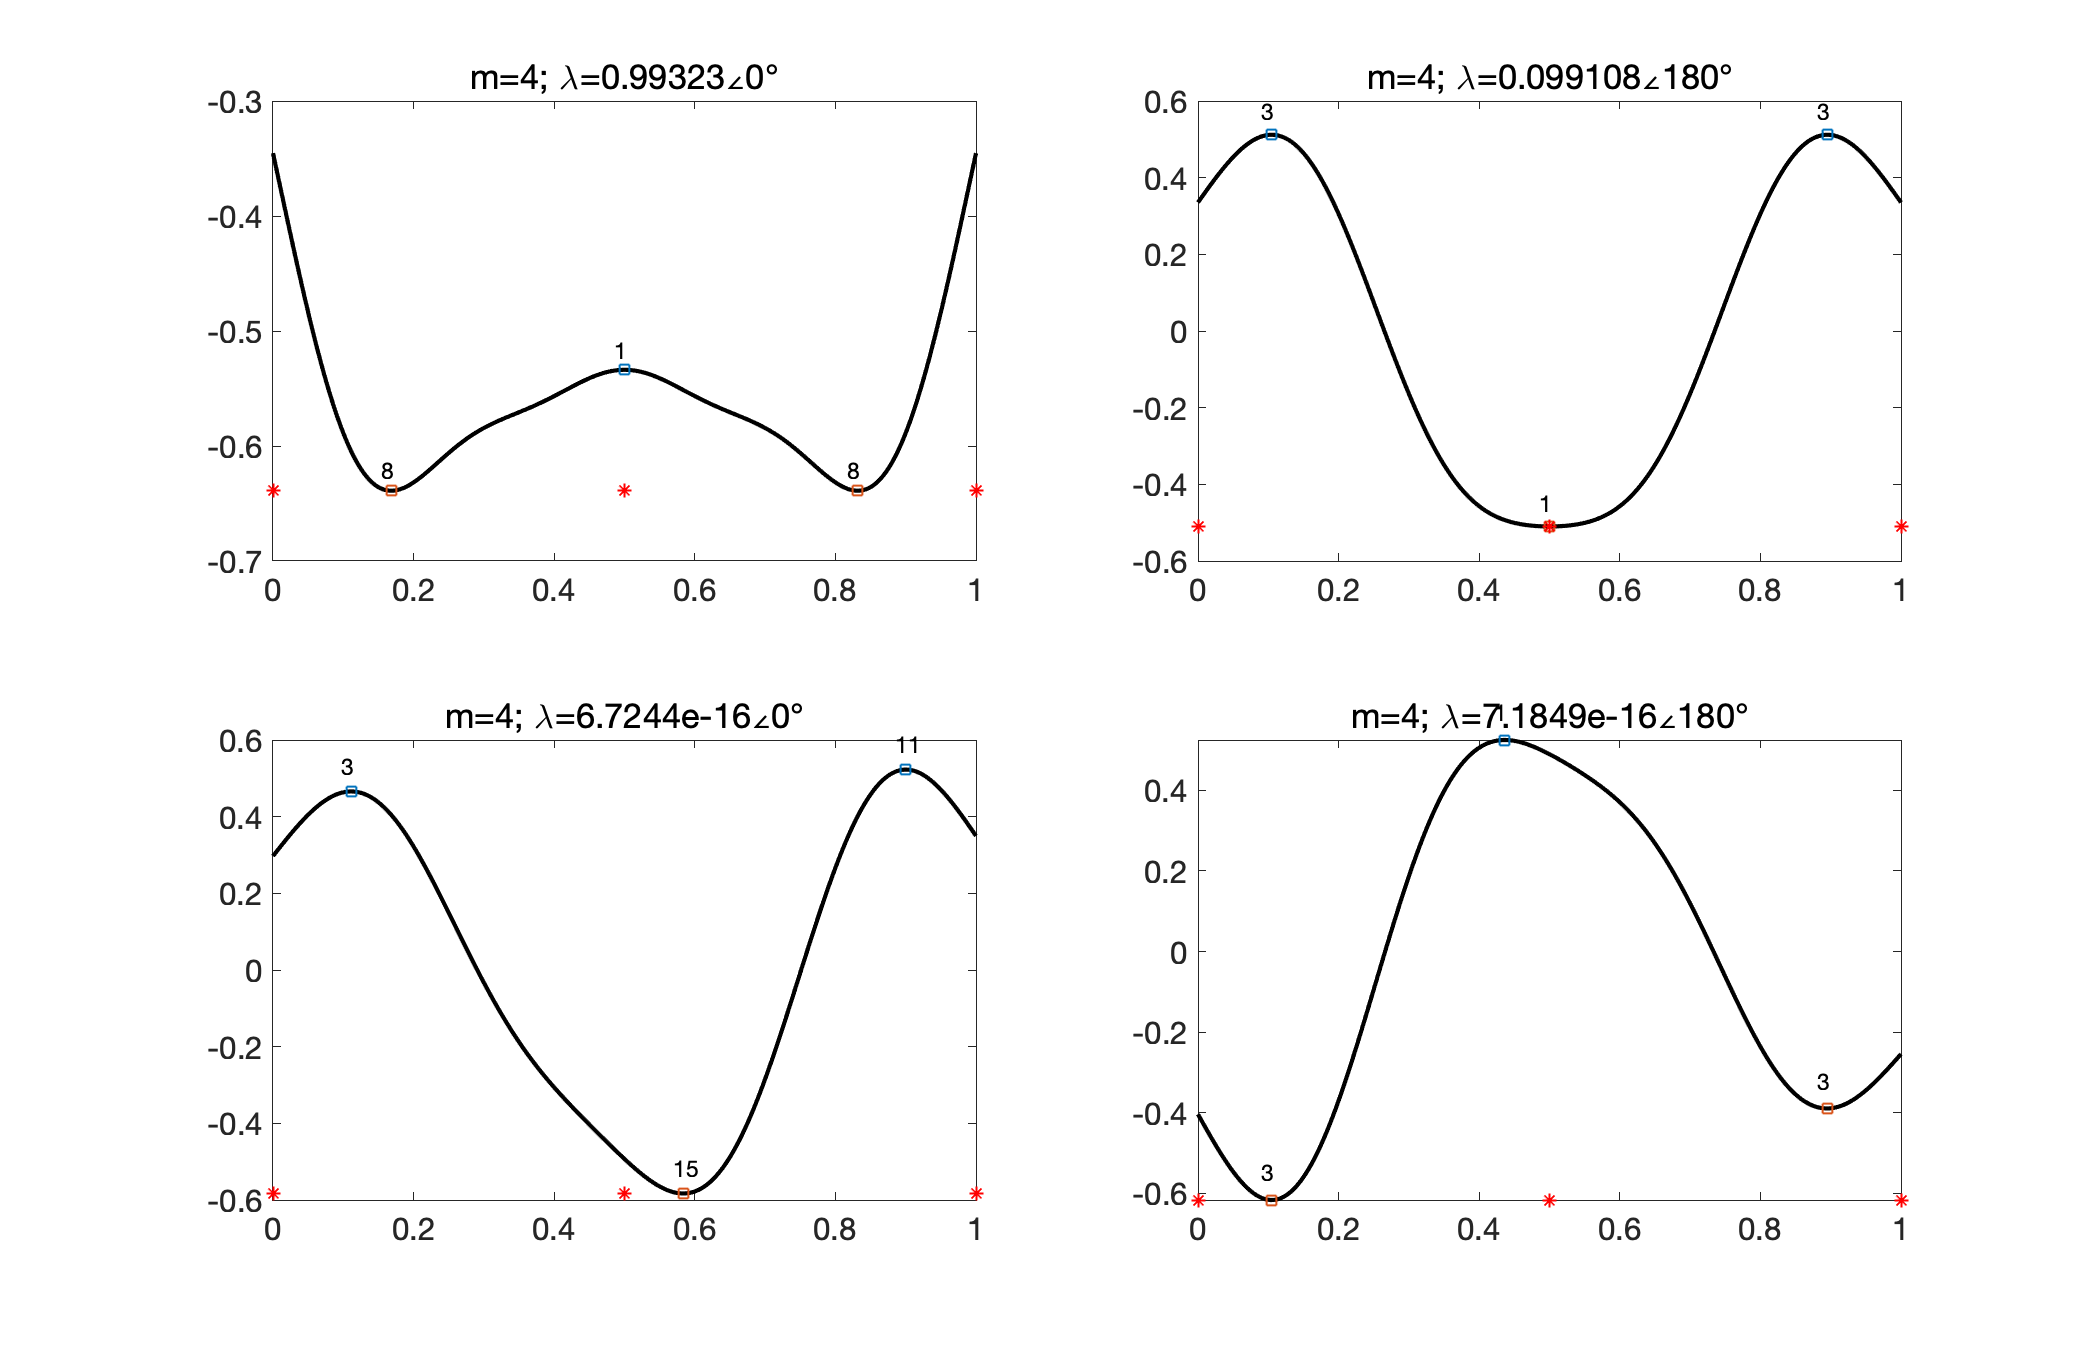
\includegraphics[scale=0.2]{tent/accurate/Tent_auto_level_n1000_m4}}
  \subfloat[m=5]{
    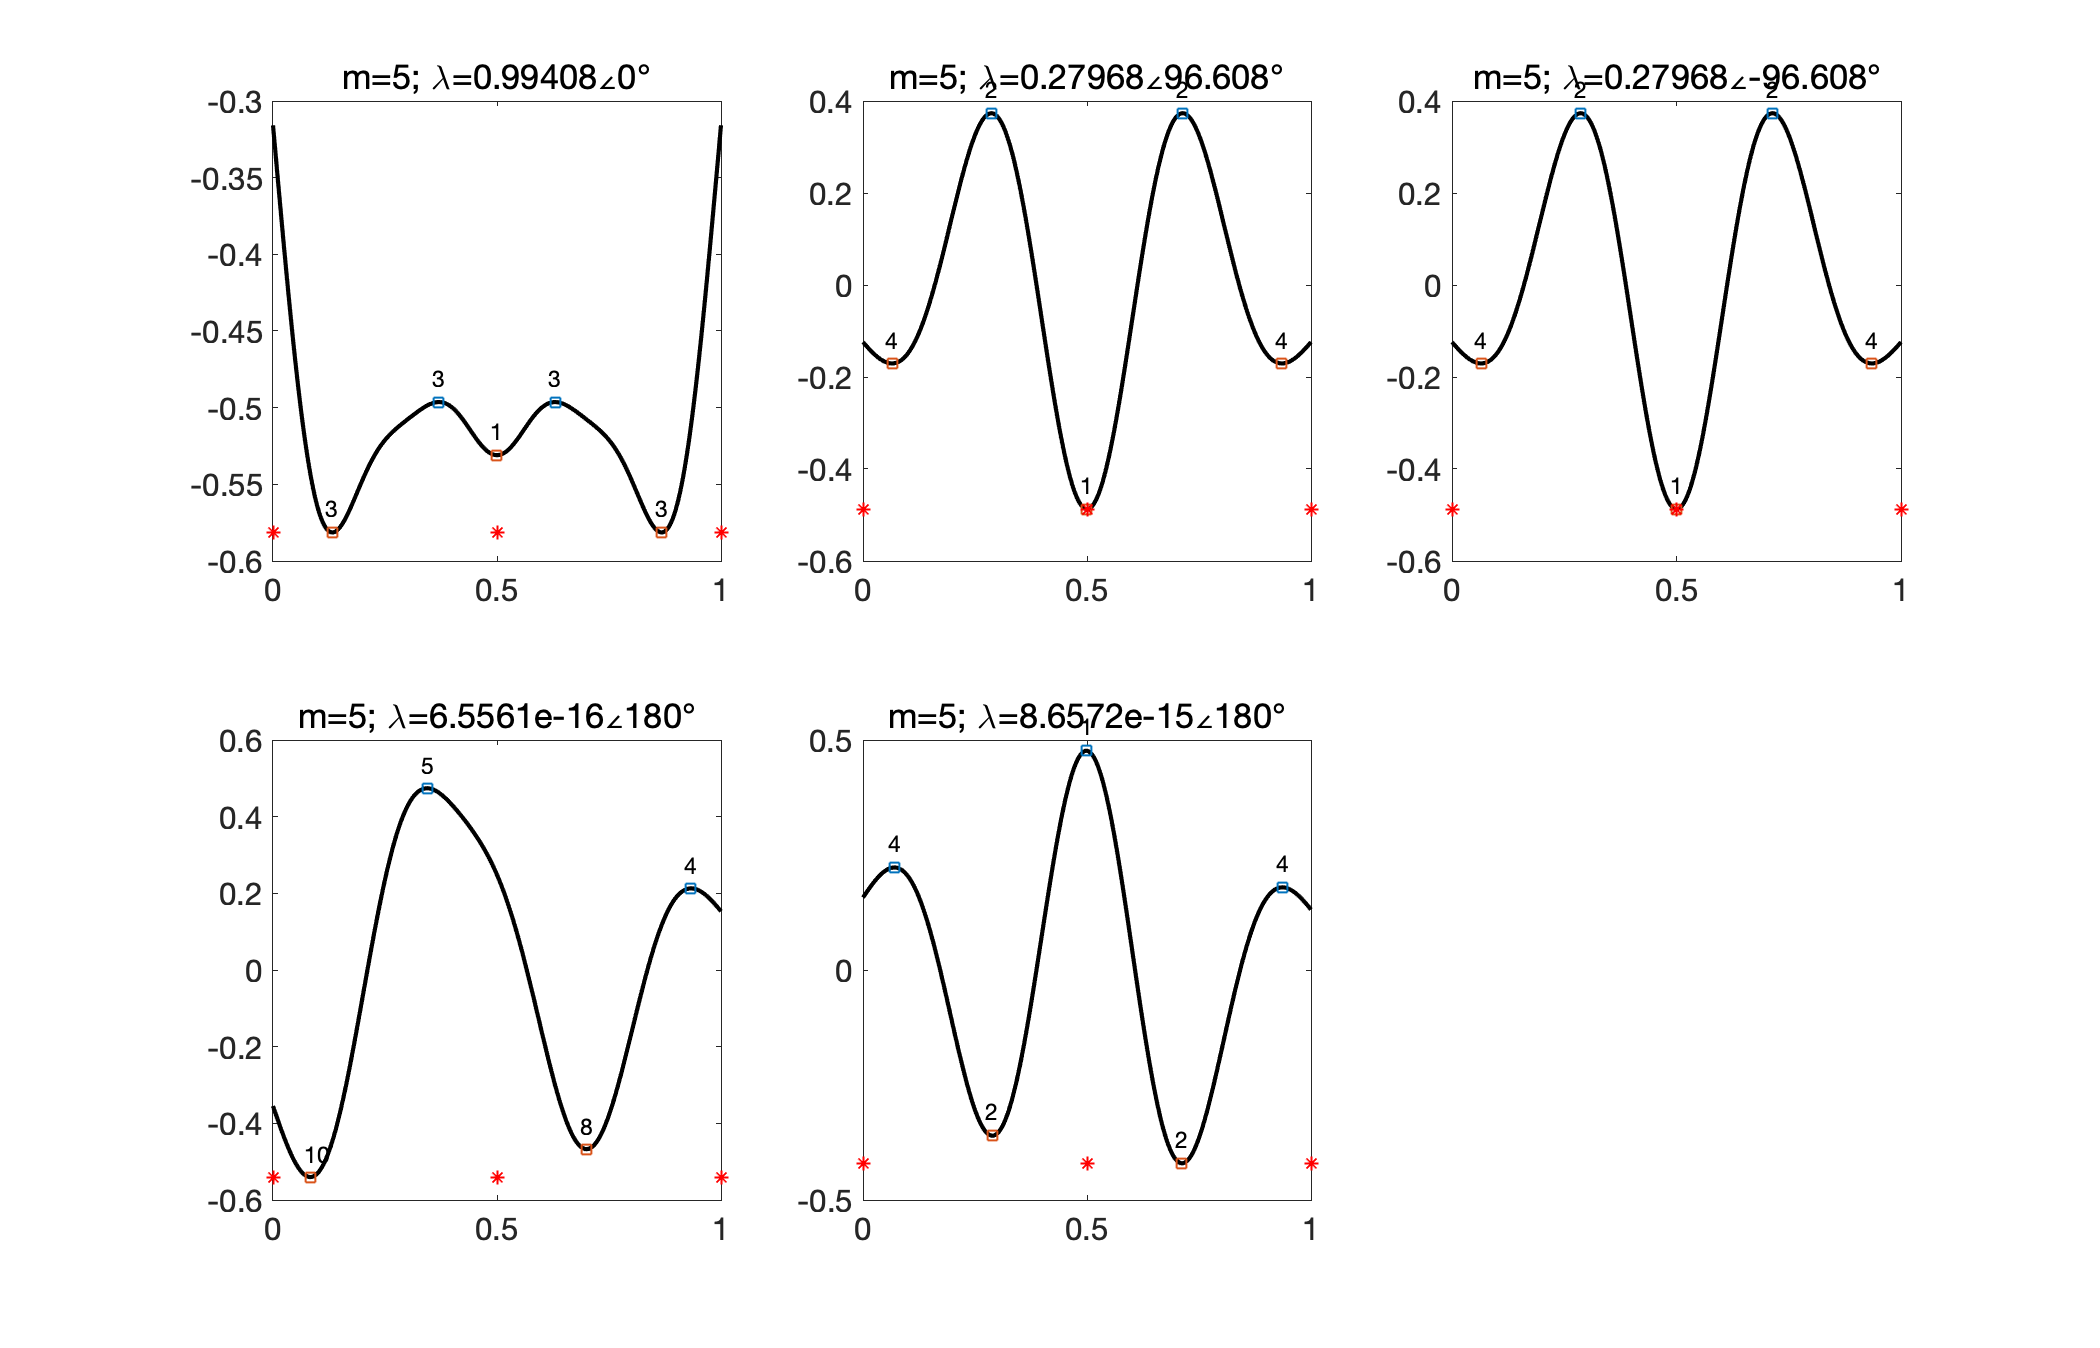
\includegraphics[scale=0.2]{tent/accurate/Tent_auto_level_n1000_m5}}
    \\
  \subfloat[m=8]{
    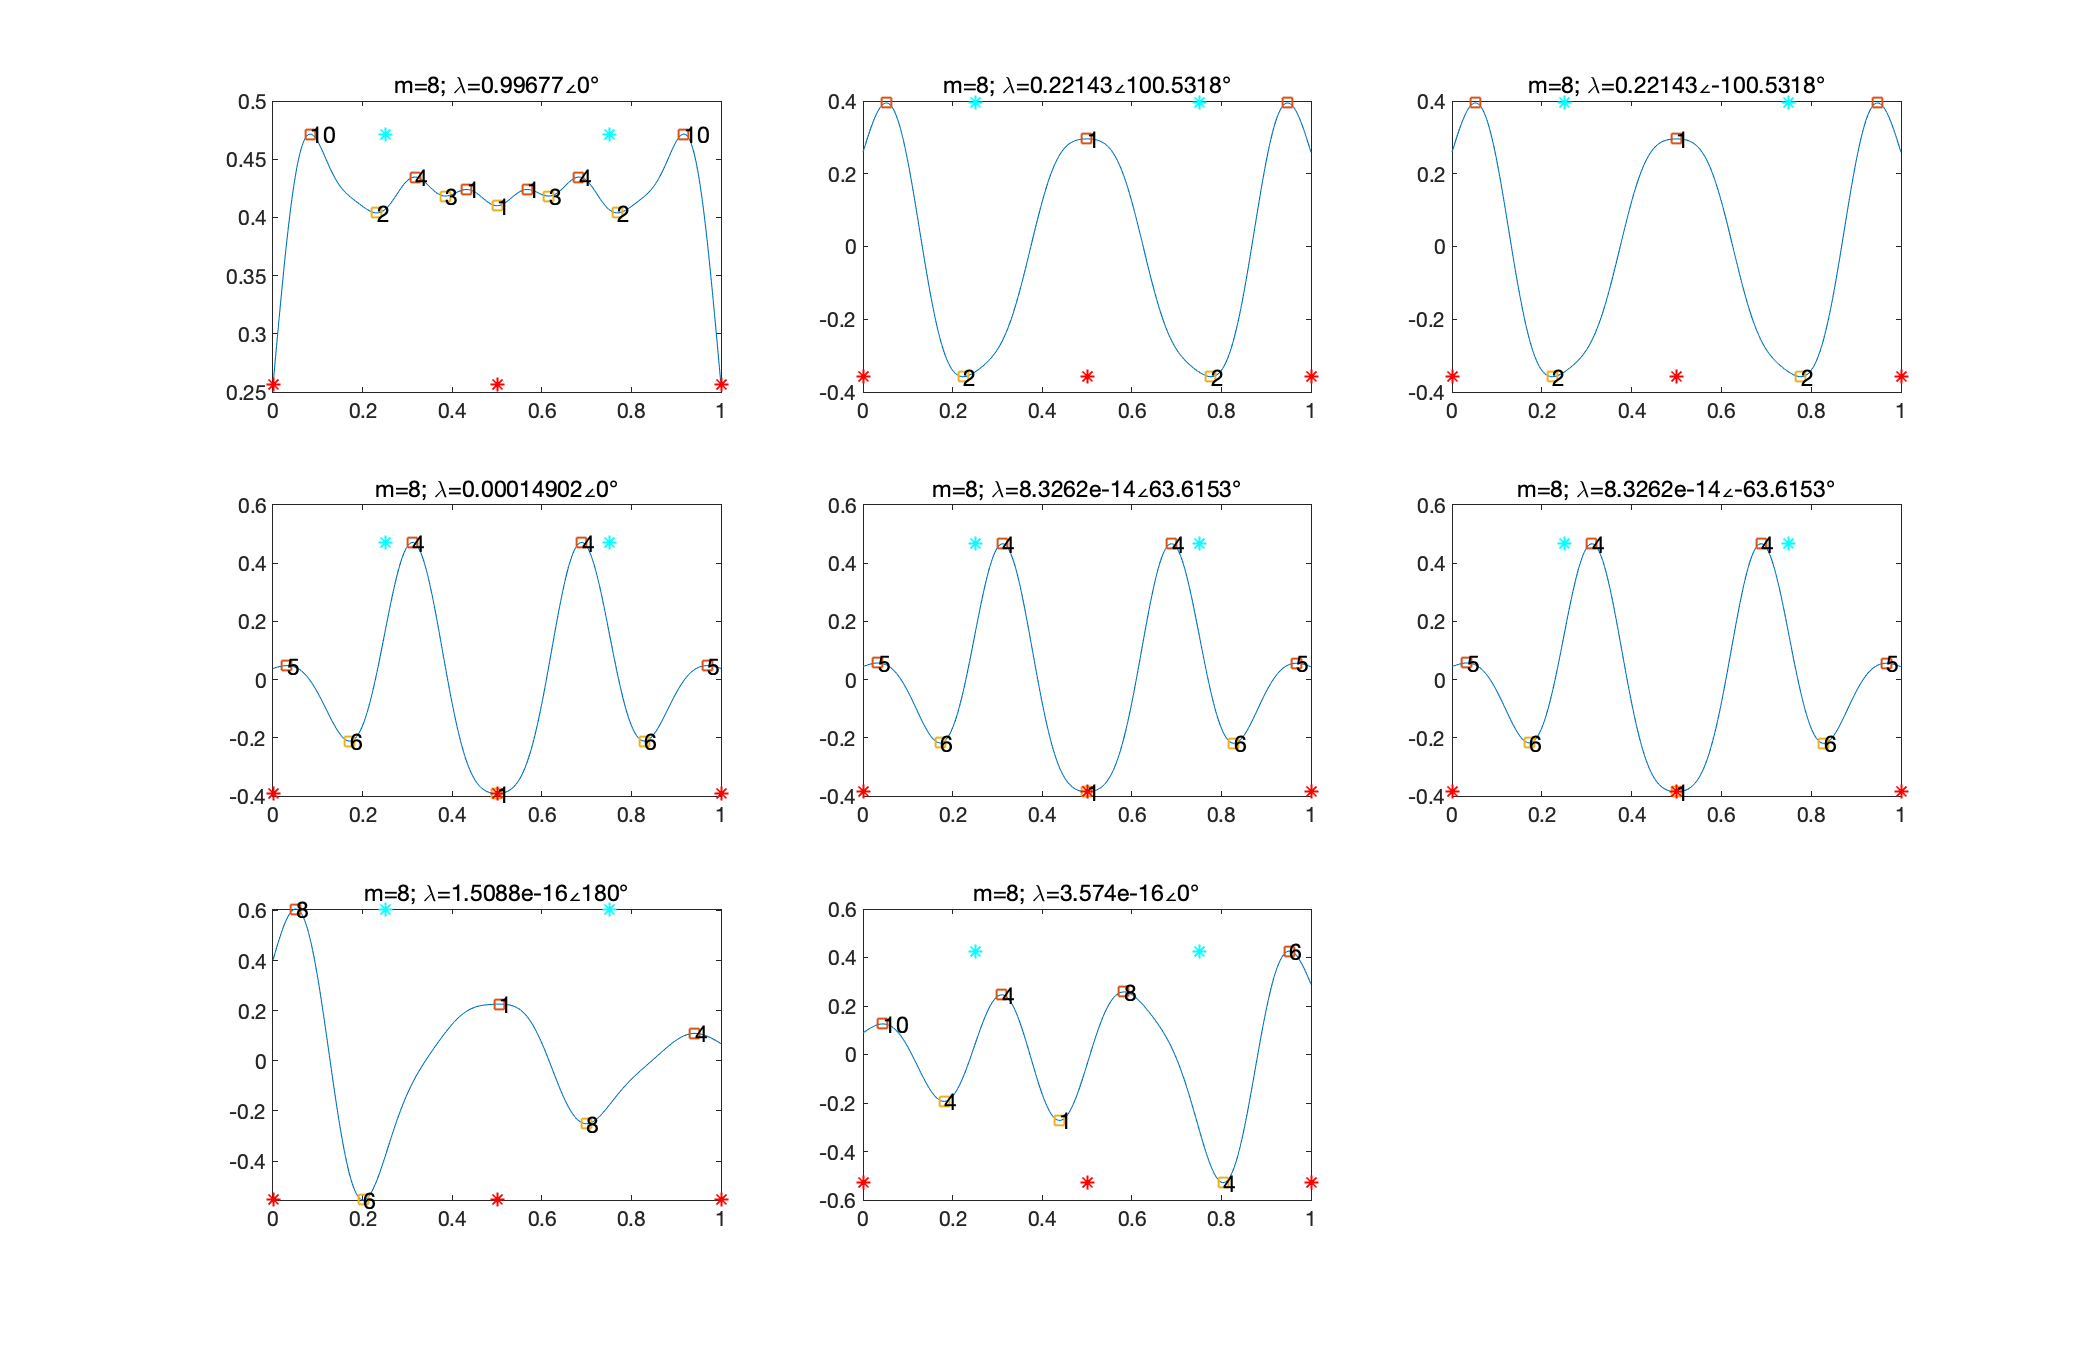
\includegraphics[scale=0.2]{tent/accurate/Tent_auto_level_n1000_m8}}
  \subfloat[m=10]{
    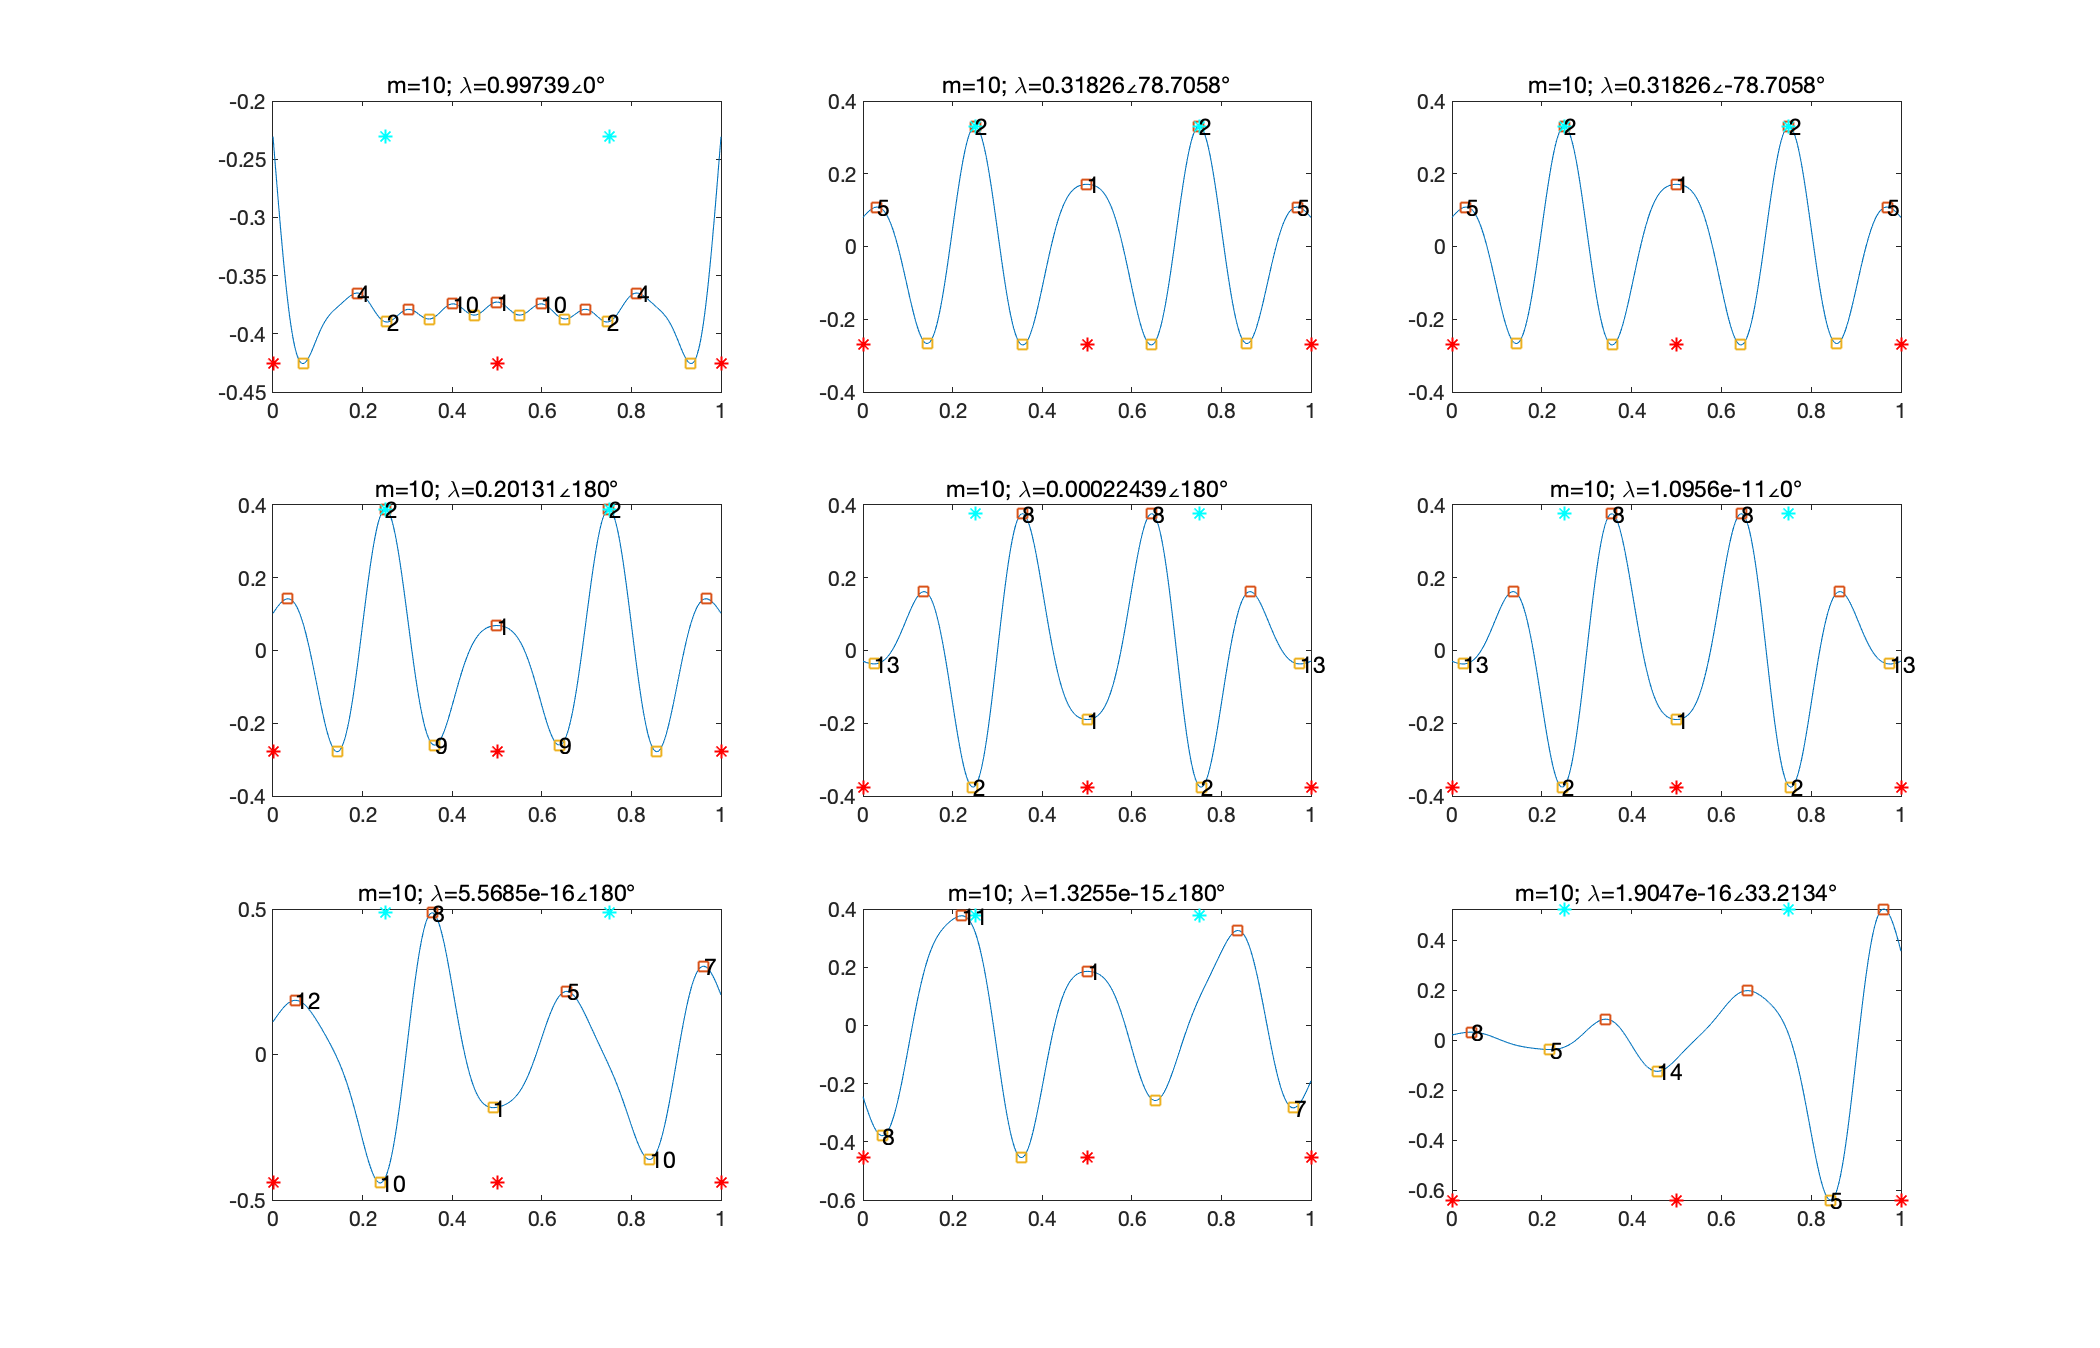
\includegraphics[scale=0.2]{tent/accurate/Tent_auto_level_n1000_m10}}
    \\
  \subfloat[m=15]{
    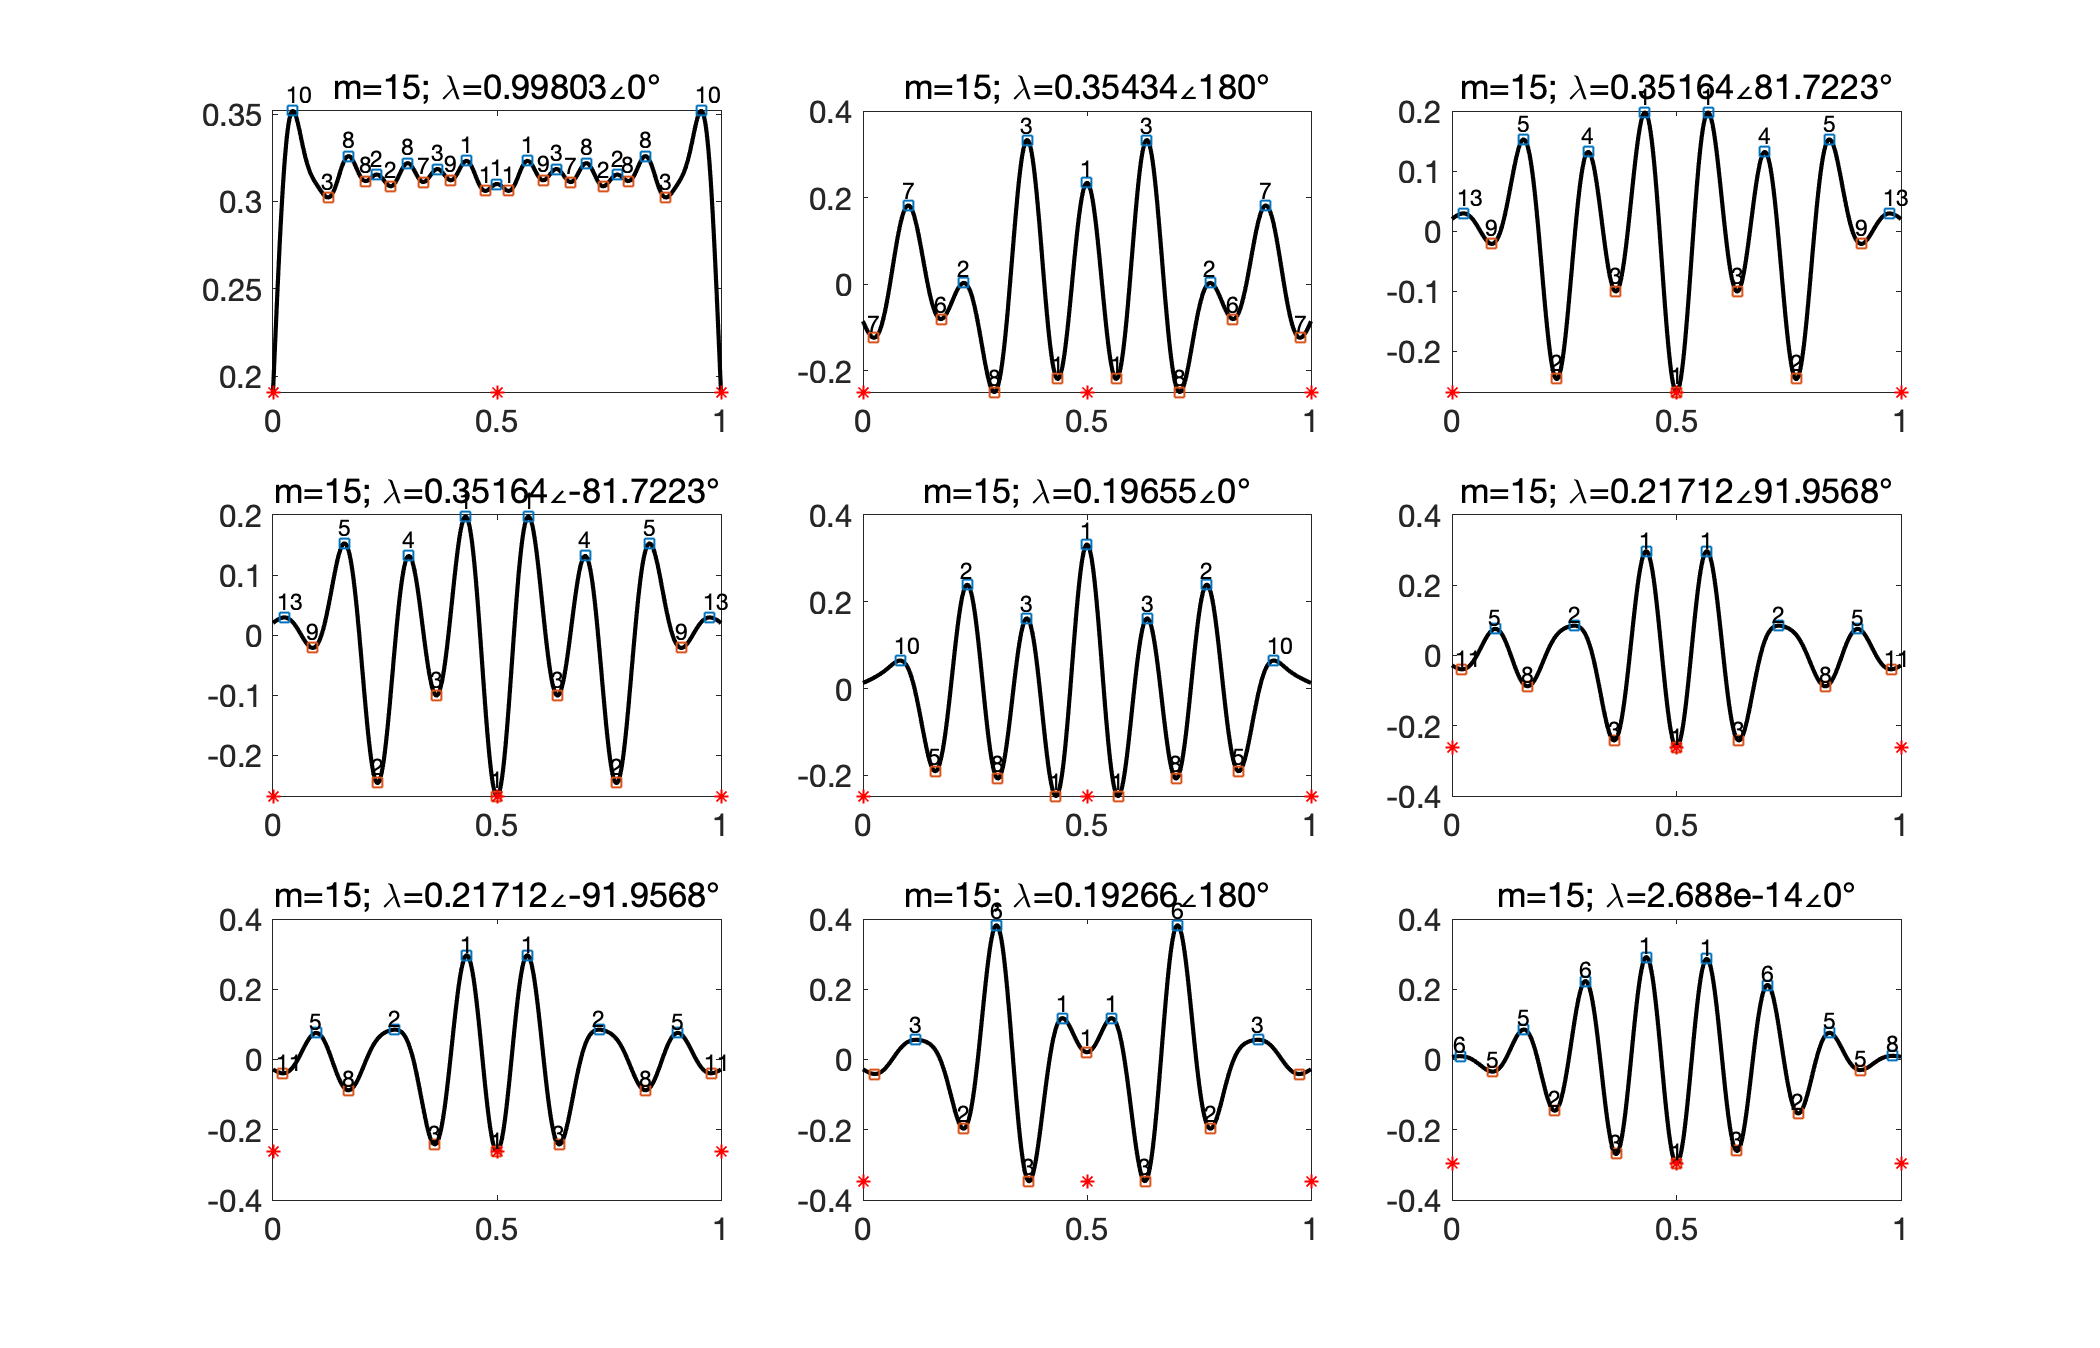
\includegraphics[scale=0.2]{tent/accurate/Tent_auto_level_n1000_m15}}
  \subfloat[m=20]{
    \includegraphics[scale=0.2]{tent/accurate/Tent_auto_level_n1000_m20}}
    \\
  \caption[帐篷映射本征函数确定边界点层次]{帐篷映射本征函数确定边界点层次($n=1000,noise=0$):红色与青色的点表示帐篷映射的边界点,空心方块表示本征函数的极值点,且若满足迭代关系则将其边界点的层次标注在极值点附近}\label{fig:Tent_auto_level_n1000_m4}
\end{figure}

在图\ref{fig:Tent_auto_level_n1000_m4}中,由于误差我们仅计算了处于层次为15以内的边界点:我们可以发现,很多本征函数的极值点,我们都可以通过迭代关系确定其层次。当然也存在一些其它无法确定的极值点,这可能与我们的数值计算误差有关,但是较关键的边界点都能较好的计算出,且我们可以识别大部分极值点。这使得我们通过Koopman算符可以对动力学系统性质的探究更深了一步:我们可以通过Koopman算符确定动力学系统的边界点,且可以通过增加函数格点数量来精确的寻找重要的边界点,而其他层次的边界点也可以通过迭代关系来确定。


\subsubsection{多峰映射}

关于Koopman算符的本征函数对帐篷映射的边界点的描述我们作了一定探究,但是其对其他系统的适用性还有待进一步讨论,我们将在后面的章节中继续讨论其他映射。在这里我们讨论一些类似于帐篷单峰映射的动力学系统:多峰映射。

多峰映射也是分段线性映射,如在两个峰的情况下,我们将其相图及含噪声的相图画出(图\ref{fig:Tents5_noise_phase_d0}),图中不同颜色的点为其不同层次性下的边界点。探究在此情形下,Koopman算符的本征函数能否描述双峰映射的边界点。

\begin{figure}[!]
  \centering
  \subfloat[noise=0]{
    \includegraphics[scale=0.2]{tent/tents/Tents5_noise_phase_d0}}
  \subfloat[noise=0.001]{
    \includegraphics[scale=0.2]{tent/tents/Tents5_noise_phase_d0-001}}
  \caption[双峰映射不同噪声下的相空间]{双峰映射不同噪声下的相空间:图中不同颜色的点为其不同层次性下的边界点}\label{fig:Tents5_noise_phase_d0}
\end{figure}

我们取演化格点数量$n=1000$,基函数数量$m=2,3,4,5,8,10,15,20$,高斯白噪声噪信幅值比$noise=0.001$,计算得Koopman算符的本征函数图像如图\ref{fig:Tents5_eigen_noise_n1000m20d0-001}。

\begin{figure}[!]
  \centering%[2,3,4,5,8,10,15,20]
  \subfloat[m=2]{
    \includegraphics[scale=0.2]{tent/tents/Tents5_eigen_noise_n1000m2d0-001}}
  \subfloat[m=3]{
    \includegraphics[scale=0.2]{tent/tents/Tents5_eigen_noise_n1000m3d0-001}}
    \\
  \subfloat[m=4]{
    \includegraphics[scale=0.2]{tent/tents/Tents5_eigen_noise_n1000m4d0-001}}
  \subfloat[m=5]{
    \includegraphics[scale=0.2]{tent/tents/Tents5_eigen_noise_n1000m5d0-001}}
    \\
  \subfloat[m=8]{
    \includegraphics[scale=0.2]{tent/tents/Tents5_eigen_noise_n1000m8d0-001}}
  \subfloat[m=10]{
    \includegraphics[scale=0.2]{tent/tents/Tents5_eigen_noise_n1000m10d0-001}}
    \\
  \subfloat[m=15]{
    \includegraphics[scale=0.2]{tent/tents/Tents5_eigen_noise_n1000m15d0-001}}
  \subfloat[m=20]{
    \includegraphics[scale=0.2]{tent/tents/Tents5_eigen_noise_n1000m20d0-001}}
    \\
    \caption[双峰映射的边界点与本征函数]{双峰映射的边界点与本征函数($noise=0.001$):不同颜色的点表示大小峰映射不同层次的边界点,空心方块表示本征函数的极值点}\label{fig:Tents5_eigen_noise_n1000m20d0-001}
\end{figure}

双峰映射的三个边界点$x=\frac{1}{4},\frac{1}{2},\frac{3}{4}$与帐篷映射的边界点相图,但在帐篷映射中其属于不同层次,但双峰映射的这三个边界点属于同一层次。但是我们同样可以在本征函数图像中找到其边界点的位置:如图\ref{fig:Tents5_eigen_noise_n1000m20d0-001}(h)第二个小图中,本征函数图像的极大值点与边界点吻合程度较好,且极小值点在一定程度上反映了其原像点的划分。这与我们之前的结论是极为相似的。

当我们的双峰映射的两个峰作出一定区别时,如将相图中第二个峰的峰值减少一半,我们将其称之为大小峰映射,其相图与韩噪声的相图如图\ref{fig:Tents5l_noise_phase_d0}所示。

\begin{figure}[!]
  \centering
  \subfloat[noise=0]{
    \includegraphics[scale=0.2]{tent/tents/Tents5l_noise_phase_d0}}
  \subfloat[noise=0.001]{
    \includegraphics[scale=0.2]{tent/tents/Tents5l_noise_phase_d0-001}}
  \caption[大小峰映射不同噪声下的相空间]{大小峰映射不同噪声下的相空间:图中不同颜色的点为其不同层次性下的边界点}\label{fig:Tents5l_noise_phase_d0}
\end{figure}

我们取演化格点数量$n=1000$,基函数数量$m=2,3,4,5,8,10,15,20$,高斯白噪声噪信幅值比$noise=0.001$,计算得Koopman算符的本征函数图像如图\ref{fig:Tents5l_eigen_noise_n1000m20d0-001}。

\begin{figure}[!]
  \centering%[2,3,4,5,8,10,15,20]
  \subfloat[m=2]{
    \includegraphics[scale=0.2]{tent/tents/Tents5l_eigen_noise_n1000m2d0-001}}
  \subfloat[m=3]{
    \includegraphics[scale=0.2]{tent/tents/Tents5l_eigen_noise_n1000m3d0-001}}
    \\
  \subfloat[m=4]{
    \includegraphics[scale=0.2]{tent/tents/Tents5l_eigen_noise_n1000m4d0-001}}
  \subfloat[m=5]{
    \includegraphics[scale=0.2]{tent/tents/Tents5l_eigen_noise_n1000m5d0-001}}
    \\
  \subfloat[m=8]{
    \includegraphics[scale=0.2]{tent/tents/Tents5l_eigen_noise_n1000m8d0-001}}
  \subfloat[m=10]{
    \includegraphics[scale=0.2]{tent/tents/Tents5l_eigen_noise_n1000m10d0-001}}
    \\
  \subfloat[m=15]{
    \includegraphics[scale=0.2]{tent/tents/Tents5l_eigen_noise_n1000m15d0-001}}
  \subfloat[m=20]{
    \includegraphics[scale=0.2]{tent/tents/Tents5l_eigen_noise_n1000m20d0-001}}
    \\
    \caption[大小峰映射的边界点与本征函数]{大小峰映射的边界点与本征函数($noise=0.001$):不同颜色的点表示大小峰映射不同层次的边界点,空心方块表示本征函数的极值点}\label{fig:Tents5l_eigen_noise_n1000m20d0-001}
\end{figure}

大小峰映射的三个边界点$x=\frac{1}{4},\frac{1}{2},\frac{3}{4}$的性质又有所不同:其每个边界点的性质都有所差异,我们也可以在本征函数图像中观察到这种差异带来的影响:本征函数关于$x=\frac{1}{2}$的对称性被破坏,且本征函数图像的趋势有所区别。如图\ref{fig:Tents5l_eigen_noise_n1000m20d0-001}(f)第三个小图中,虽然在$x=\frac{1}{4}$与$x=\frac{3}{4}$边界点处都存在本征函数的极值点,但极值点的大小和曲率都所有差异,我们可以通过这种差异来确定这两点性质的差异。

%\subsection{小结}

\clearpage
\section{一维离散映射系统:Logistic映射}
Logistic映射是研究动力系统、混沌、分形等复杂系统的一个经典模型,其来源于生态学中的虫口模型,用以描述种群的变化。Logistic映射从数学形式上来看是一个非常简单的混沌映射,但却有极其复杂的动力学行为,在保密通信领域的应用十分广泛。

Logistic是一个定义在$x\in [0,1]$的一维离散的动力系统,其动力学方程可描述为
\begin{equation}
    x_{n+1}=f(x_n)=\gamma x_n(1-x_n),\ x_n\in [0,1], n=1,2,3,\cdots
\end{equation}
Logistic映射存在两个不动点:$x_1^*=0$和$x_2^*=1-\frac{1}{\gamma}$。Logistic映射的相图描述了相空间的映射关系:
\begin{figure}
	\centering
	\includegraphics[scale=0.6]{logistic_phase.png}
    \caption{Logistic映射的相图($\gamma=4$)}
    \label{fig:logi_pha}
\end{figure}

Logistic映射的动力学过程可以看作是在一维相空间上的拉伸再折叠的过程。通过非线性动力学的知识可以得到,该系统在$\gamma$取不同值时表现出不同的动力学行为。当$0<\gamma<1$时,系统最终都会渐进的趋于0;当$1<\gamma<3$时,系统会收敛到一个不动点,该不动点的值为$x^*=(\gamma-1)/\gamma$,此时系统的极限行为会趋于该不动点的值;当$3<\gamma<3.57$时,系统的迭代会出现周期行为,随着$\gamma$的增大,周期的长度也会相应的增加,例如2周期,4周期,8周期轨道等,直到大约为$\gamma=3.57$时,周期的长度趋于无穷大;当$3.57<\gamma<4$时,系统的迭代会在周期类型和混沌类型之间来回切换,且大部分区域呈现混沌状态;直到$\gamma=4$时,系统处于完全混沌的状态。

Logistic映射的分岔图$x_n-\gamma$描述了系统随$\gamma$表现出的不同的动力学行为:
\begin{figure}
	\centering
	\includegraphics[scale=1]{logistic_bifurcation.png}
    \caption{Logistic映射的分岔图($2.6\leqslant\gamma\leqslant 4$)}
    \label{fig:logi_pha}
\end{figure}

李雅普诺夫指数是描述混沌现象的一个重要的指标,Logistic映射的李雅普诺夫指数图像$\lambda-\alpha$如下图所示:
\begin{figure}
	\centering
	\includegraphics[scale=0.2]{logistic_lypn.png}
    \caption{Logistic映射的李雅普诺夫指数}
    \label{fig:logi_lypn}
\end{figure}
根据李雅普诺夫指数的性质:当$\lambda<0$时,映射系统收敛于某一不动点;当$\lambda=0$时,系统进行周期运动;当$\lambda>0$时,系统处于混沌状态。我们可以同样得到在$3.57<\gamma<4$区域,系统处于混沌状态(在$\gamma=3.83$处存在一三周期轨道),当$\gamma=4$时系统处于混沌状态。

不失一般性,在我们的Koopman分析中,我们取$\gamma=4$的一个特例,通过Logistic映射的动力学方程演化出一系列的数据,作为Koopman分析的源数据,以此来分析Logistic映射的系统特征。
\clearpage
\section{二维离散映射系统:埃农映射}

\subsection{埃农映射的动力学过程}

埃农(Henon)映射是1976年由法国数学家Michel H\'{e}non提出的。Henon映射是一种可以产生混沌现象的离散映射系统。最近,用埃农映射产生的混沌序列进行图像加密的报道逐渐增多。埃农映射的迭代方程可以描述为

\begin{equation}
    \begin{cases}
        x_{n+1}=y_n+1-ax_n^2\\
        y_{n+1}=bx_n
    \end{cases}\ x,y\in [-1.5,1.5]
\end{equation}

其只有一个非线性项,埃农映射的映射过程可以分解为非线性弯曲、x方向压缩、对称变换三个子过程。其三个过程的子映射可以分别写为:
\begin{equation}
    \begin{aligned}
        T_1: & \begin{cases}
            x'=x\\
            y'=1-ax^2+y
        \end{cases}\\
        T_2: & \begin{cases}
            x''=bx'\\
            y''=y'
        \end{cases}\\
        T_3: & \begin{cases}
            x'''=y''\\
            y'''=x''
        \end{cases}
    \end{aligned}
\end{equation}

埃农映射存在两个不动点:$x^*=\dfrac{b-1\pm\sqrt{(b-1)^2+4a}}{2a},y^*=bx^*$。在经典的埃农映射中,我们通常取$a=1.4$与$b=0.3$,此时该映射出现奇怪吸引子并表现出混沌现象,在该参数下,埃农映射的吸引子和不动点如下图:
\begin{figure}
	\centering
	\includegraphics[scale=0.8]{henon_phase.png}
    \caption{埃农映射的吸引子和不动点($a=1.4,b=0.3$)}
    \label{fig:logi_lypn}
\end{figure}

在我们的Koopman分析中,我们在取上述参数值的情况下,通过Henon映射的迭代方程演化出一系列的数据,作为Koopman分析的源数据,以此来分析Henon映射的系统特征。


\subsection{埃农映射的Koopman算符本征函数}
\subsubsection{正交完备基函数空间}
\begin{figure}
    \centering
    \subfloat[高斯基函数]{
      \includegraphics[scale=0.4]{henon/Henon_eigen_Gauss_n100m50md45}}
    \\
    \subfloat[傅里叶基函数]{
      \includegraphics[scale=0.4]{henon/Henon_eigen_Fourier_n100m50}}
    \caption{埃农映射不同基函数的本征函数}
\end{figure}

\begin{figure}
    \centering
    \subfloat{
      \includegraphics[scale=0.2]{henon/Henon_eigen_Gauss_n100m50md45_figure1}}
    \subfloat{
      \includegraphics[scale=0.2]{henon/Henon_eigen_Gauss_n100m50md45_figure2}}
    \\
    \subfloat{
      \includegraphics[scale=0.2]{henon/Henon_eigen_Gauss_n100m50md45_figure3}}
    \subfloat{
      \includegraphics[scale=0.2]{henon/Henon_eigen_Gauss_n100m50md45_figure4}}
    \\
    \subfloat{
      \includegraphics[scale=0.2]{henon/Henon_eigen_Gauss_n100m50md45_figure5}}
    \subfloat{
      \includegraphics[scale=0.2]{henon/Henon_eigen_Gauss_n100m50md45_figure6}}
    \\
    \subfloat{
      \includegraphics[scale=0.2]{henon/Henon_eigen_Gauss_n100m50md45_figure7}}
    \subfloat{
      \includegraphics[scale=0.2]{henon/Henon_eigen_Gauss_n100m50md45_figure8}}
    \\
    \caption{埃农映射不同本征值的本征函数($n=100^2$,$m=50^2,d_j=\frac{3}{45}$)}
\end{figure}

\subsubsection{自然基函数空间}
\begin{figure}
    \centering
    \subfloat{
      \includegraphics[scale=0.2]{henon/natural/Henon_eigen_natural_n2000m4_figure1}}
    \subfloat{
      \includegraphics[scale=0.2]{henon/natural/Henon_eigen_natural_n2000m4_figure2}}
    \\
    \subfloat{
      \includegraphics[scale=0.2]{henon/natural/Henon_eigen_natural_n2000m4_figure3}}
    \subfloat{
      \includegraphics[scale=0.2]{henon/natural/Henon_eigen_natural_n2000m4_figure4}}
    \\
    \caption{埃农映射自然基函数下的本征函数($n=2000$,$m=4$)}
\end{figure}

\begin{figure}
    \centering
    \subfloat[m=1]{
      \includegraphics[scale=0.2]{henon/natural/Henon_eigen_natural_n2000m1}}
    \subfloat[m=2]{
      \includegraphics[scale=0.2]{henon/natural/Henon_eigen_natural_n2000m2}}
    \\
    \subfloat[m=3]{
      \includegraphics[scale=0.2]{henon/natural/Henon_eigen_natural_n2000m3}}
    \subfloat[m=4]{
      \includegraphics[scale=0.2]{henon/natural/Henon_eigen_natural_n2000m4}}
    \\
    \subfloat[m=5]{
      \includegraphics[scale=0.2]{henon/natural/Henon_eigen_natural_n2000m5}}
    \subfloat[m=6]{
      \includegraphics[scale=0.2]{henon/natural/Henon_eigen_natural_n2000m6}}
    \\
    \subfloat[m=7]{
      \includegraphics[scale=0.2]{henon/natural/Henon_eigen_natural_n2000m7}}
    \subfloat[m=8]{
      \includegraphics[scale=0.2]{henon/natural/Henon_eigen_natural_n2000m8}}
    \\
    \caption{埃农映射自然基函数不同基函数数量下的本征函数($n=2000$)}
\end{figure}

\begin{figure}
	\centering
	\includegraphics[scale=0.4]{henon/natural/Henon_eigen_natural_n2000}
    \caption{埃农映射自然基函数不同基函数数量下的本征函数($n=2000$)}
\end{figure}

\subsubsection{吸引子上的本征函数}

\begin{figure}
    \centering
    \subfloat[俯视图]{
      \includegraphics[scale=0.4]{henon/Henon_eigen_Gauss_attr_n6245m50md45}}
    \\
    \subfloat[鸟瞰图]{
      \includegraphics[scale=0.4]{henon/Henon_eigen_Gauss_attr_n6245m50}}
    \\
    \caption{埃农映射高斯基函数下在吸引子上的本征函数($n=6245$,$m=50^2,$,$d_j=\frac{3}{45}$)}
\end{figure}

\begin{figure}
    \centering
    \subfloat[m=2]{
      \includegraphics[scale=0.28]{henon/Henon_eigen_Gauss_attr_leftU_n6245m2}}
    \\
    \subfloat[m=3]{
      \includegraphics[scale=0.28]{henon/Henon_eigen_Gauss_attr_leftU_n6245m3}}
    \\
    \subfloat[m=4]{
      \includegraphics[scale=0.28]{henon/Henon_eigen_Gauss_attr_leftU_n6245m4}}
    \\
    \caption{埃农映射高斯基函数下在吸引子上的本征函数($n=6245$)}
\end{figure}


\subsection{Koopman算符对埃农映射的相空间划分}
\subsubsection{埃农映射在吸引子上的划分}
\begin{table}[]
    \centering
    \begin{tabular}{|c|c|c|}
    \hline
        & 横坐标x & 纵坐标y  \\ \hline
    1   & 0.7021 & -0.0044 \\ \hline
    2   & 0.7986 & 0.0019  \\ \hline
    3   & 1.2307 & -0.0249 \\ \hline
    4   & 1.2717 & -0.0205 \\ \hline
    \end{tabular}
    \caption{埃农映射的边界点}
\end{table}

\begin{figure}
	\centering
	\includegraphics[scale=0.6]{henon/attractors/Henon_boundary}
    \caption{埃农映射的边界点}
\end{figure}

\begin{figure}
    \centering
    \subfloat[正向迭代]{
      \includegraphics[scale=0.4]{henon/attractors/Henon_boundary_forward}}
    \subfloat[反向迭代]{
      \includegraphics[scale=0.4]{henon/attractors/Henon_boundary_reverse}}
    \caption{埃农映射的边界点及其像点、原像点}
\end{figure}

\begin{figure}
    \centering
    \subfloat[m=1]{
      \includegraphics[scale=0.2]{henon/attractors/Henon_eigen_natural_attr_n2000m1}}
    \subfloat[m=2]{
      \includegraphics[scale=0.2]{henon/attractors/Henon_eigen_natural_attr_n2000m2}}
    \\
    \subfloat[m=3]{
      \includegraphics[scale=0.2]{henon/attractors/Henon_eigen_natural_attr_n2000m3}}
    \subfloat[m=4]{
      \includegraphics[scale=0.2]{henon/attractors/Henon_eigen_natural_attr_n2000m4}}
    \\
    \subfloat[m=5]{
      \includegraphics[scale=0.2]{henon/attractors/Henon_eigen_natural_attr_n2000m5}}
    \subfloat[m=6]{
      \includegraphics[scale=0.2]{henon/attractors/Henon_eigen_natural_attr_n2000m6}}
    \\
    \subfloat[m=7]{
      \includegraphics[scale=0.2]{henon/attractors/Henon_eigen_natural_attr_n2000m7}}
    \subfloat[m=8]{
      \includegraphics[scale=0.2]{henon/attractors/Henon_eigen_natural_attr_n2000m8}}
    \\
    \caption{埃农映射的边界点与本征函数对吸引子的划分($n=2000$)}
\end{figure}

\begin{figure}
	\centering
	\includegraphics[scale=0.4]{henon/attractors/Henon_eigen_natural_attr_n2000}
    \caption{埃农映射的边界点与本征函数对吸引子的划分($n=2000$)}
\end{figure}

\subsubsection{埃农映射的周期轨道}
\begin{figure}
	\centering
	\includegraphics[scale=0.4]{henon/period/Henon_periodic_orbits}
    \caption{埃农映射的周期轨道}
\end{figure}

\begin{figure}
    \centering
    \subfloat[T=2]{
      \includegraphics[scale=0.2]{henon/period/Henon_eigen_Gauss_period_n100m50T2}}
    \subfloat[T=4]{
      \includegraphics[scale=0.2]{henon/period/Henon_eigen_Gauss_period_n100m50T4}}
    \\
    \subfloat[T=6]{
      \includegraphics[scale=0.2]{henon/period/Henon_eigen_Gauss_period_n100m50T6}}
    \subfloat[T=7]{
      \includegraphics[scale=0.2]{henon/period/Henon_eigen_Gauss_period_n100m50T7}}
    \\
    \caption{埃农映射的本征函数与周期轨道($n=100^2$,$m=50^2,d_j=\frac{3}{45}$)}
\end{figure}

\begin{figure}
	\centering
	\includegraphics[scale=0.4]{henon/period/Henon_eigen_Gauss_period1_n100m50T12}
    \caption{埃农映射的本征函数与周期轨道(T=12)}
\end{figure}


\subsubsection{埃农映射的不稳定流型}

\begin{figure}
	\centering
	\includegraphics[scale=0.4]{henon/manifold/Henon_iter_reverse_forward}
    \caption{埃农映射的迭代}
\end{figure}
\begin{figure}
	\centering
	\includegraphics[scale=0.4]{henon/manifold/Henon_eigen_Gauss_manifold_n100m50}
    \caption{埃农映射的迭代与本征函数}
\end{figure}
\begin{figure}
	\centering
	\includegraphics[scale=0.4]{henon/manifold/Henon_eigen_Gauss_manifold_n100m50T4}
    \caption{埃农映射的不稳定流型与本征函数(T=4)}
\end{figure}

\begin{figure}
    \centering
    \subfloat{
      \includegraphics[scale=0.2]{henon/manifold/Henon_eigen_Gauss_manifold_n100m50T7_1}}
    \subfloat{
      \includegraphics[scale=0.2]{henon/manifold/Henon_eigen_Gauss_manifold_n100m50T7_2}}
    \\
    \subfloat{
      \includegraphics[scale=0.2]{henon/manifold/Henon_eigen_Gauss_manifold_n100m50T7_3}}
    \subfloat{
      \includegraphics[scale=0.2]{henon/manifold/Henon_eigen_Gauss_manifold_n100m50T7_4}}
    \\
    \caption{埃农映射的不稳定流型与本征函数(T=7)}
\end{figure}

\subsection{更多的讨论}

\subsection{小结}
\clearpage
\section{三维连续时间系统:洛伦兹系统}
洛伦兹(Lorenz)系统是1963年由Edward Lorenz提出的描述空气流体运动的一个数学模型。1998年,S.Smale提出21世纪的18个著名的数学问题,其中第14个问题就是关于洛伦兹系统的研究。迄今为止,对洛伦兹系统的研究无论是从数学、物理还是工程上都是十分重要的问题。洛伦兹系统的动力学方程表示为:
\begin{equation}
    \begin{cases}
        \dot{x}=\sigma(y-x)\\
        \dot{y}=x(\rho-z)-y\\
        \dot{z}=xy-\beta z
    \end{cases}\
\end{equation}

该方程描述了一个三维相空间的三个分量对时间的变化率。其中$x$代表对流强度,$y$代表上升流和下降流的温差,$z$代表铅直方向温度分布的非线性强度。$c$是Rayleigh数,为系统的主要控制参数,$a$是Prandt数,$b$是外形比。Lorenz系统具有非线性、非周期性和确定性的性质。参数$\sigma$,$\rho$,$\beta$取不同值时Lorenz系统表现出不同的动力学行为。如在$\rho<1$时,系统只有一个不动点,即原点,所有轨道的长期行为都趋于原点;当$\rho=1$时系统发生了叉式分岔,在$\rho>1$时出现了两个不动点,不动点的稳定性可由其他参数满足的条件确定。三个不动点的坐标分别为$(0,0,0)$、$(\sqrt{\beta(\rho-1)},\sqrt{\beta(\rho-1)},\rho-1)$、$(-\sqrt{\beta(\rho-1)},-\sqrt{\beta(\rho-1)},\rho-1)$。当我们将三个参数取一组特定的值$\rho=28$,$\sigma=10$,$\beta=8/3$时,Lorenz方程的解是混沌的,相空间会存在两个奇异吸引子。

洛伦兹系统的这种动力学特征用传统的非线性动力学知识是比较难分析的,其相图如下:
\begin{figure}
	\centering
	\includegraphics[scale=0.8]{lorenz_phase.png}
    \caption{洛伦兹系统的相图($\rho=28$,$\sigma=10$,$\beta=8/3$)}
    \label{fig:lorz_phas}
\end{figure}
在洛伦兹系统中,所有的非平衡解最终趋向同一个复杂的集合,这就是所谓的洛伦兹吸引子。我们将在取上述参数的条件下,通过Lorenz微分方程演化出相空间的一条轨道,作为Koopman分析的源数据,以此来分析Lorenz系统的特征。



%% 本章参考文献
% \ifx\usechapbib\empty
% \nocite{BSTcontrol}
% \setcounter{NAT@ctr}{0}
% \bibliographystyle{buptgraduatethesis}
% \bibliography{references}
% \fi
